\documentclass[a5paper,12pt,openany]{book}
%\usepackage{extsizes}

\usepackage[top=2cm,bottom=2cm,bindingoffset=0cm]{geometry}

\usepackage{mathtext}
\usepackage{makeidx}

\usepackage{longtable}
\usepackage[tc]{titlepic}

\usepackage{fontspec}
\usepackage[protrusion=true,expansion,tracking=true]{microtype}

\usepackage{titlesec, blindtext, color}


\definecolor{gray75}{gray}{0.75}

%\newcommand{\hsp}{\hspace{20pt}}

%\titleformat{\chapter}[hang]{\Huge\bfseries}{\thechapter\hsp\textcolor{gray75}{|}\hsp}{0pt}{\Huge\bfseries}


\newcommand{\hsp}{\hspace{20pt}}

%\titleformat{\chapter}[hang]{\Huge\bfseries}{\thechapter\hsp\textcolor{gray75}{|}\hsp}{0pt}{\Huge\bfseries}


\titleformat{\chapter}[hang]{\Huge\bfseries}{\thechapter\hsp\textcolor{gray75}{|}\hsp}{0pt}{\Huge\bfseries}

\usepackage[toc,titletoc]{appendix}
\renewcommand\appendixtocname{Приложения}
\renewcommand\appendixpagename{Приложения}

\usepackage{xltxtra}

\usepackage{polyglossia}
\setmainlanguage{russian}
\setotherlanguage{ukrainian}
\setotherlanguage{english}
\setotherlanguage{greek}
\setotherlanguage{latin}


%\setromanfont{DejaVu Serif}
%\setsansfont{DejaVu Sans}
%\setmonofont{DejaVu Sans Mono}

%\setmainfont{DejaVuSerif.ttf}
%\setromanfont{DejaVuSerif.ttf}
%\setsansfont{DejaVuSans.ttf}
%\setmonofont{DejaVuSansMono.ttf}



\setmainfont[BoldFont={DejaVuSerif-Bold.ttf},
ItalicFont={DejaVuSerif-Italic.ttf},
 BoldItalicFont={DejaVuSerif-BoldItalic.ttf}]{DejaVuSerif.ttf}

\setromanfont[BoldFont={DejaVuSerif-Bold.ttf},
ItalicFont={DejaVuSerif-Italic.ttf},
 BoldItalicFont={DejaVuSerif-BoldItalic.ttf}]{DejaVuSerif.ttf}

\setsansfont[BoldFont={DejaVuSans-Bold.ttf},
ItalicFont={DejaVuSans-Oblique.ttf},
 BoldItalicFont={DejaVuSans-Oblique.ttf}]
{DejaVuSans.ttf}

\setmonofont[BoldFont={DejaVuSansMono-Bold.ttf},
ItalicFont={DejaVuSansMono-Oblique.ttf},
 BoldItalicFont={DejaVuSansMono-BoldOblique.ttf}]
{DejaVuSansMono.ttf}


\usepackage{indentfirst} 

\usepackage{verse}

\usepackage{graphicx}

\usepackage[pdfpagelabels,unicode,plainpages=false]{hyperref}

\hypersetup{pdftitle=Словарь киеведа. Петр Семилетов}

\usepackage{bookmark} 
\usepackage{relsize}

\usepackage{tocloft,calc}
\usepackage[nottoc,numbib]{tocbibind}

\usepackage{multicol}


\frenchspacing
\righthyphenmin=2

\renewcommand{\chaptername}{}
\renewcommand{\thechapter}{}


\newcommand\myimgprefix{s-}

%\titlepic{\includegraphics[width=0.50\textwidth]{pix/obl02.jpg}}

\title{Словарь киеведа}

\author{Петр Семилетов}
\date{05/04/2025}

\usepackage[svgnames]{xcolor}

\newcommand*{\plogo}{\fbox{$\mathcal{PL}$}} 

%----------------------------------------------------------------------------------------
%	TITLE PAGE
%----------------------------------------------------------------------------------------

\newcommand*{\titleAT}{\begingroup % Create the command for including the title page in the document
\newlength{\drop} % Command for generating a specific amount of whitespace
\drop=0.1\textheight % Define the command as 10% of the total text height

\rule{\textwidth}{1pt}\par % Thick horizontal line
\vspace{2pt}\vspace{-\baselineskip} % Whitespace between lines
\rule{\textwidth}{0.4pt}\par % Thin horizontal line

\vspace{\drop} % Whitespace between the top lines and title
\centering % Center all text
\textcolor{Red}{ % Red font color
{\Huge Словарь киеведа}\\[0.5\baselineskip] % Title line 1
%{\Large и}\\[0.75\baselineskip] % Title line 2
%{\Huge Киева}
} % Title line 3

\vspace{0.25\drop} % Whitespace between the title and short horizontal line
\rule{0.3\textwidth}{0.4pt}\par % Short horizontal line under the title

\mbox{ }\\
редакция 6.1\\

\vspace{\drop} % Whitespace between the thin horizontal line and the author name


{\Large \textsc{Петр Семилетов}}\par % Author name

\vfill % Whitespace between the author name and publisher text
%{\large \textcolor{Red}{\plogo}}\\[0.5\baselineskip] % Publisher logo
{\large \textsc{Киев 2025}}\par % Publisher

\vspace*{\drop} % Whitespace under the publisher text

\rule{\textwidth}{0.4pt}\par % Thin horizontal line
\vspace{2pt}\vspace{-\baselineskip} % Whitespace between lines
\rule{\textwidth}{1pt}\par % Thick horizontal line

\endgroup}


\begin{document}

\pagestyle{empty}

\titleAT

\newpage

%\pagestyle{headings}


%\maketitle 

\pagestyle{empty}

\tableofcontents

\pagestyle{plain}



%\mainmatter

\chapter*{Предисловие}
\markboth{\MakeUppercase{Предисловие}}{}
\addcontentsline{toc}{chapter}{Предисловие}

Эта книга родилась из приложения к моей «Ереси о Киеве» – некоторые читатели помнят там эдакий словарик в конце, исчезнувший в одной из редакций книги. На деле он не исчез, а был отведен в сторонку и стал дополняться, превращаясь в самостоятельный труд.

Я не очень люблю справочники, они разрушают пространственное представление о местности, ибо сведения в них упорядочены по алфавиту, а не, допустим, с юга на север или с запада на восток. Однако упорядочение по алфавиту позволяет быстро найти нужную статью.

«Словарь киеведа» – книга неправильная, неправильная по названию и по содержимому. Название засело у меня в голове и никак не менялось, поэтому я решил оставить его как есть. 

Что до изложенных в словаре сведений, то это самый неполный и неряшливый справочник из всех возможных, частью похожий на заметки на полях, сделанные для себя самого. Я никоим образом не ставил целью охватить все урочища Киева, все местные названия, все исчезнувшие или существующие поныне здания. Более того, некоторые вещи я нарочно не занес в словарь, поскольку более подробно описал их в других краеведческих книгах моего пера. Это служит постоянной причиной моей неудовлетворености словарем. Итак, если нечто большое и важное упомянуто в словаре кратко, вроде Демиевки, скорее всего это означает, что сему отведено много места в прочих моих работах.

Благодарю всех кто снабжал меня разными местными названиями, а кроме «всех» – поименно родителей, Настю, Колю Арестова и его маму, а также Дашу Кононюк. Много полезного сообщили зрители «Киевской амплитуды» и «Планеты Киева» на Ютубе – спасибо вам!

«Словарь киеведа» набран в разрабатываемом мною текстовом редакторе TEA, свёрстан в системе вёрстки LaTeX (с движком lualatex), и всё это разумеется в операционной системе Linux.

Новые редакции книги, по мере их выхода, будут выкладываться на моем сайте:\\ 
\href{http://semiletov.org}{http://semiletov.org}\\
Либо на странице \href{https://orcid.org/0009-0002-3901-7785}{https://orcid.org/0009-0002-3901-7785}\\
Ну или просто еще где-нибудь в сети, например на телеграм-канале Киевоград - \href{t.me/kievograd}{t.me/kievograd}\\

Буду рад отзывам и дополнениям по электронной почте: \href{mailto:peter.semiletov@gmail.com}{peter.semiletov@gmail.com}\\
в Телегу: @petersemiletov


\part{Левый берег}

\chapter*{А}
\addcontentsline{toc}{chapter}{А}

\textbf{Алексеевская слободка} –  дореволюционное официальное название слободки на Трухановом острове.

Слободка возникла при пароходных мастерских (верфях) 1-го и 2-го Пароходного обществ – последние находились в самой южной части острова, на месте бывшего кирпичного завода. Хотя рабочие обжили остров еще с середины 19 века, официальное разрешение селиться там Дума выдала лишь в 1907-м. 

На слободке была Базарная (или Запорожская) площадь, и улицы Полтавская, Конотопская и Днепровская.

Островом заправлял магнат Давид Марголин, на его дачу туда провели в 1895 году телефон, зато никакого мостового сообщения с Киевом не было, только переправа да зимой по льду.

Для слободки Марголин построил за 30000 рублей в 1909 году двухклассное училище - каменное здание\footnote{50°27'51"N 30°32'9"E} о двух этажах, с мастерской на первом. Во дворе находился дом для сотрудников училища.

Тогда же на деньги Марголина начали возводить и церковь св. Елизаветы\footnote{50.46440010881086, 30.534080357262944}, по проекту епархиального архитектора Евгения Ермакова (закладка 21 сентября 1909, освящение 2 сентября 1910), при участии Елизаветы Треповой, жены генерал-губернатора Трепова. Иконостас выполнен художником Александром Александровичем Мурашко. Священником во время благоденствия храма в 1911-1917 годах служил Евгений Константинович Эргардт\footnote{Из списка духовенства Киева на 1914 год: Елизаветинская церковь (Труханов остров). Наст. свящ. Эргардт Евг. Кон., псал. Бурковский Ксен. Тим., стар. Карпенко Стеф. Фом.}, будущий (в 1920-х) настоятель Екатерининской церкви на Лукьяновском кладбище. Закрыта в 1934 году и переделана под общагу для работников телефонной станции, сгинула вместе с остальными постройками слободки, когда ее подожгли немцы осенью 1943 года. Фундаменты сохранились.

Напротив Почтовой площади, чуть ниже по течению Днепра на Трухановом был парк Эрмитаж с кафешантанным театром, а выше, напротив Борисоглебской церкви – яхт-клуб\footnote{50.46887568134493, 30.534606733683923}.\\

\medskip

\textbf{Аварийный поселок}

Известен также как Поселок аварийщиков и Немецкий квартал. Бешеными темпами исчезающий райончик желтоватых домиков в 2-3 этажа между Соцгородом и линией метро около станции Черниговская. Прежде ограничивался улицами Красногвардейской, Попудренко, Минина, Красноткацкой. 

Был застроен известными домиками в 1947-52 годах для рабочих близлежащих заводов ДШК, «Радикал» и «Химволокно», сначала пленными, а затем уже вольнонаемными немцами. Однако еще в 1935 году «хутор Аварийный» был включен в состав Дарницкого района Киева, и на карте того времени на месте нынешнего Аварийного – пустыри Дарницких лагерей, а вот вдоль восточной стороны улицы Магнитогорской стояли какие-то домики. К 1944 году на месте нынешнего Аварийного поселка, между Краковской и Попудренко, уже было десятка два жилых домиков. От Броварского шоссе они отделялись лесочком. Северо-восточной стороной тот поселок граничил с грунтовой дорогой (нынешняя Красногвардейская улица), дальше за которой шли пески с сосняком, такая же местность была и на юго-запад, где сейчас улица Пожарского. Тогда же в классическом Соцгороде, в конце современных Краковской и Попудренко уже возникли большие дома, например Краковская 5, Попудренко 20 и 18-А, Строителей 34/1.

Сносить Аварийный поселок или отдельные дома собирались еще в 1970-е, но взялись кажется с половины 2008 года. Первыми жертвами пали здания по Красноткацкой и вдоль Красногвардейской (до Краковской), где на месте снесенных домов воздвигли высотки. С 2016 новая застройка поползла по самой Краковской.\\

\medskip

\textbf{Аврора} – небольшой парк на Воскресенке. В западной его части по 2005 год стоял одноименный кинотеатр, теперь на его месте ТРЦ. Широкоэкранный кинотеатр на 800 мест был построен в 1966 году. Фасад над входом украшало мозаичное панно, изображавшее девушку с факелом в руке, на фоне крейсера Авроры, впрочем революционную девушку можно было считать и богиней Авророй, как кому угодно. Кинотеатр перестал показывать фильмы еще в начале-середине девяностых.

В парке находится разворотное кольцо трамваев 8 и 22, что идут на Позняки и ЖБК (завод Железобетонных конструкций).\\

\medskip

\textbf{Алмазное озеро}

50.50642318333851, 30.64834934308184

Крупнейшее озеро в Киеве, примыкает к северной части Лесного кладбища, занимает существенно углубленное добычей сначала торфа, а потом песка русло болота Куричева, давнего рукава Десны. До углубления, в 20 веке народное название местности было Торфы. Имя свое озеро получило от завода «Алмаз» (ныне Монетный двор) на северном берегу озера.

Полумесяц Алмазного продолжается на север болотом, тоже остатком русла Десны. На северо-восточном его берегу, на поросших сосной, песчаных Сторожевых горах, стоит ТЭЦ-6, вероятно там же располагался один из летописных Городков. Сторожевые горы отделяют это болото от другого – частично осушенного, истощенного торфодобычей болота Ковпыт, что некогда соединялось каналом с Куричевым.

Северо-западный и западный берега озера – равнинны, а южный, юго-восточный и восточный представляют – гора, где растут сосны, а кое-где тополями. Гора то пологая, то местами с высокими песчаными обрывами – точно как известный «классический» современный берег Десны. 

На озере есть остров, отделенный от берега проливом.

Длина озера около 3,5 километров, ширина около 600 метров. Глубина достигает 35-40 метров, что вызвано добычей тут песка.

В озеро с северной стороны впадает ручей, текущий вдоль заболоченной части озера и дороги у подножия Сторожевых гор, со стороны ТЭЦ-6.

На южном берегу озера, в некотором отдалении от воды, находится Лесное кладбище, отгороженное от соснового леса сетчатым забором. Среди покрытых хвоей дюн за этой оградой можно найти обломки надгробных памятников.\\

\medskip

%\textbf{Алто, Олто} – старое название Борисполя.

\textbf{Алмазный}, пионерлагерь

50°23'25"N 30°43'21"E

Бывший пионерлагерь у северной окраины Бортничей, в Никольском лесу, у речки Демидовки.

В пионерлагере был свой сад. В 1970-х руководил лагерем Леонид Вацлавович Конисевич, воспитанник коммуны Макаренко. Сюда приезжали как советские школьники, так и заграничные – от шотландских профсоюзов, из Польши и других стран.

В середине 90-х в лагере жили офицеры-студенты из Института МВД (на Коллекторной улице).

На 2010-е, на территории работал вероятно филиал психбольницы имени Павлова – реабилитировали наркоманов и вроде бы пациентов с тяжелыми расстройствами психики.

\chapter*{Б}
\addcontentsline{toc}{chapter}{Б}

\textbf{БВС} – народное название бульвара Верховного совета в Соцгороде. Когда идешь по бульвару от проспекта Гагарина, то раньше прямо по курсу было видно Лавру на правом берегу, а сейчас обзор заслоняет ЖК, выстроенный вместо молокозавода.

Как дорога, БВС существовал уже в 1930-е, будучи разделительной линией между полосой леса с юга и пустошами с севера, и относился к территории Дарницких военных лагерей (до революции – лагерь юнкерского училища). Современное название носит с 1949 года. Застроен в основном панельными хрущевками с тихими, зелеными дворами. В западном конце есть несколько домов сталинской эпохи, один такой слывет Розовым домом.

Последними номерами (восточная сторона улицы) БВС выходит к проспекту Юрия Гагарина, и там в доме 31 дробь 1 с советских времен по 2020 год сохранялся спортивный магазин «Олимпиец».

Начало бульвара упирается в железную дорогу, огороженную бетонной стеной, впрочем оборудован переезд, через него люди ходят на Левобережку.

К востоку от рельсов, вдоль улицы Марины Расковой (ведущей к Левобережке) с 2018 года земля застроена ЖК «Галактика», на месте корпусов молокозавода №2, который был запущен в 1961 году, а в 1995 превратился в «Галактон». После ряда перепродаж завод соединился с «Даноном», а в 2015 производственные мощности были перенесены в Кременчуг и Херсон.\\

\medskip

\textbf{Белый дом} – дом на улице Юности, 8/2, у перекрестка с Космической. Называется так по виду и дал народное имя маршруточной остановке (обычный городской транспорт по этой узкой улице с односторонним движением не ходит). Иногда говорят еще – Серый дом. \\

\medskip

\textbf{Березник} – хутор, давший имя району Березняков. В первой половине 20 века находился между улицами Серафимовича, Березняковской (вдоль железной дороги), Бучмы и озером Тельбин. Кроме Тельбина, на хуторе было множество других озер.

Тельбин (остатки одноименной речки, а вернее пролива) тогда начинался от нынешнего проспекта Воссоединения, и даже севернее, от дома номер 11 на улице Энтузиастов на Русановке, перерезанный насыпью дороги, где потом возник проспект. А на месте детсада номер 577 были воды Тельбина!

Южнее хутора, Тельбин перерубила железная дорога, отделив от него Нижний Тельбин, тогда имевший, как и верхний, долгое русло как у луговой речки.

Хуторское кладбище\footnote{50°26'16.1"N 30°36'42.7"E} было на возвышенном поле-пустыре около нынешнего пересечения проспекта Воссоединения и улицы Березняковской, около моста.

На немецкой карте 1943 года, в хуторе Березник обозначены следующие улицы: 

Шевченко – примерно нынешние адреса Тычины 7, 11, 26. Судя по одному письму 1945 года, в то время хутор Березняк воспринимался местными как Кухмистерская слободка, ибо они считали улицу Шевченко – что она в слободке, и на конвертах так писали.

Железнодорожная – шла по восточному берегу озера Тельбин, в современной южной его половине. Югом упиралась в железную дорогу.

Коротенко – перпендикулярно примыкала к Железнодорожной, а начиналась там, где ныне пустырь между домами 12 и 16 на Березняковской. Этой восточной частью улица упиралась в железную дорогу.

Заозерная – находилась между Шевченко и Коротенко, параллельно им. Востоком примыкала к железной дороге.

Хутор ограничивался с востока и юга железной дорогой, с запада – Тельбином, с севера – Наводницким шоссе.

Первым высотным домом, построенным уже на жилмассиве Березняки, было здание на нынешней Бучмы, 1. Новая улица тогда называлась Разливной. Тельбин верхом достигал окрестностей этого дома, постепенно озеро засып\'али, изгоняя к югу.\\

\medskip

\textbf{Берёзка} 

50°32'23"N   30°32'25"E

Заброшенная (на 2020) база отдыха на острове Муромец, на западном берегу длинного озера-старицы Кинище. Три ряда домиков, всего около двадцати штук. Относится к ведомству Боярского отделения связи.\\

\medskip

\textbf{Берёзка}, оно же Веселка, озеро.

50°27'47"N 30°40'27"E

Большой проточный водоем в лесу между Быковней и ДВРЗ, представляет собой пруд на речке Дарнице, расчищенный в 1954 году работниками ДВРЗ. На берегу есть лодочная станция и кафе. К озеру ведут грунтовые дороги. Глубина мне неизвестна, однако в озере тонут купальщики.

Из озера вода дальше течет по двум руслам. Одно, Дарницкий мелиоканал, следует на запад, затем на юг и на запад к Днепру. Более-менее лежит в исторической пойме реки Дарницы. А другое, Северодарницкий мелиоканал – на северо-запад, через Быковню, затем на север вдоль Лесного массива, и потом на запад в Воскресенский коллектор, через который попадает в залив Десёнку (отличается от одноименного рукава) на Радужном массиве. 

В Северодарницкий канал включен и ручей, питающий пруды в парке Победы – сей ручей тоже попадает в итоге в Воскресенский коллектор, исчекая из цепи прудов и каналом пройдя по лесу вдоль улицы Курнатовского от клиники на Алишера Навои, 1 до морга и роддома на П. Запорожца. Поэтому диггерские слухи о том, что в ручей спускают некие стоки из морга лишены оснований, ибо морг находится ближе к месту, где ручей скрывается в подземный коллектор, \\

\medskip

\textbf{Берики} – народное название Березняков.\\

\medskip

\textbf{Берковищина}, залив – примыкает к пересечению Днепровской набережной и 
улицы Анны Ахматовой.\\

\medskip

\textbf{Бетонка} – несколько небольших бетонных блоков около высотки по адресу Милютенко, 17В. Служит местом, где собираются потусить школьники.\\

\medskip

\textbf{Большая поляна}

50°29'26.7"N 30°39'24.5"E

Народное название здоровенной поляны на восток от Лесного массива, южнее Алмазного озера. На картах ошибочно подписывается как урочище Куричево, хотя Куричево – это как раз Алмазное озеро и есть. Поляна есть осушенное болото, а в лиственном лесу на запад от луговины до сих пор можно найти места, где следы от шагов в черной торфянистой почве наполняются водой. С востока к поляне подступает березняк, с севера – хвойный лес. Очень зеленое место, с густым разнотравьем, местами очень высоким.

Прежнее болото было соединено каналом с истинным болотом Куричевым, превратившимся в Алмазное озеро. Канал сохранился слева от дороги, как идти от Большой поляны к озеру.

На Большой поляне собирают целебные травы, в березняке у окраины устраивают пикники, а иногда снимают кино.\\

\medskip

\textbf{Боярское}, урочище - западный берег озера Малиновки, между озером и Чертороем. Занято дачами мелкого калибра и коттеджами, которые проиросли на месте оных дач.\\

\medskip

%\textbf{Бортничи}

\textbf{БСП} – больница скорой помощи на улице Братиславской. Выходить однако на остановке «Медучилище», ибо напротив больницы расположено это самое медучилище, а рядом еще и «Центр Сердца» – все эти здания съели часть близлежащего осколка соснового леса.\\

\medskip

\textbf{Будища} – урочище в селе Выгуровщине, ныне занято троещинской улицей Будищанской.\\

\medskip

\textbf{Буратино} – советский магазин культтоваров на проспекте Воссоединения, 14. Ныне не существует.\\

\medskip

\textbf{Быковня} – поселок около Киева на восток от Лесного массива, недолго идти пешком через березняк да сосняк или по Броварскому шоссе. Застроен в основном частными домами, однако есть несколько многоэтажек.

До революции, тогдашний хутор Быковня относился к Броварской волости Острожского уезда. На 1858 год насчитывал 3 двора. В 1897 году тут было 35 душ. В 1938 году Быковню включили в городскую черту.
 
Изначально Быковня лежала вдоль дороги, ныне Броварского проспекта или шоссе. На тридцатые годы 20 века не было улиц Путивльской, Кисловодской, Бобринецкой – дома стояли именно вдоль шоссе, а в месте присоединения к нему нынешней Кузбасской улицы находилось озеро, по обе стороны от шоссе. Сейчас там под дорогой проходит часть Северодарницкого мелиоканала от озера Березки, так что давнее озеро лежало на месте этого проложенного несколько позже канала. Подробнее о мелиоканале читайте в моей «Ереси о Киеве».
   
Вообще Быковню окружали болот – с юга Пляховские, что развились в пойме речки Дарницы, а на западе болото занимало окрестности угла между улицами Жукова и Матеюка (с озером на месте станции метро Лесная, озеро тоже было по обе стороны от шоссе). По 2000 годы сохранялось болотце на север от Быковнянского кладбища, там даже бабка пасла стадо коз, но ко второму десятилетию 21 века болотце высохло. Кладбище старое, на немного возвышенном по отношению к болоту пригорке, показано еще на картах 19 века. Отгорожено от леса бетонным забором.

Перпендикулярно к «старой» Быковне примыкает возникший в 1950-х поселок Радистов с улицами Радистов и Ушицкой, построенный для служащих радиостанции. 

В начале Ушицкой расположена заброшенная территория передающего радиоцентра в/ч А-0799 – тут были казармы, гараж, командный пункт и бомбоубежище. На 2021 год сохранились остатки полуразобранных зданий и КПП. Году эдак в 2006 воинская часть еще стояла сохранной за сетчатым забором с колючей проволокой. Дорожки были аккуратно заметены, деревья побелены. Потом дорожки засыпала хвоя, ограда покосилась, и началось расхищение бесхозной собственности.

В другом конце поселка Радистов на 2021 год есть закрытый, полузаброшенный радиопередающий цех №1 Киевского радиопередающего центра, то есть аппаратная часть радиостанции, с охлаждающими резервуарами для некогда стоявших тут высоких (до 110 метров) мощных антенн. Внутри и снаружи – повышенный радиационный фон.

Центр работал с 1953 по 1998 год. К антеннам были подключены ламповые передатчики «Снег», вещавшие в КВ и СВ диапазонах. Могли держать связь, например, с атомными ледоколами. Некоторые считают, однако, что центр играл роль обычной глушилки вражеских голосов.

В нулевых на запад от поселка Радистов в лесу лежало множество полуразобранных автомобилей, как понимаю ворованных.

Из достопримечательностей Быковни отмечу церковь святого мученика Иоанна Воина, расположенную в синем железнодорожном вагоне. Я видел вагоны-гаражи на ДВРЗ, но вот церковь в вагоне прежде никогда.

В Быковне прожил последние годы жизни актер Борислав Брондуков – из поселка родом его жена Катерина.\\

\chapter*{В}
\addcontentsline{toc}{chapter}{В}

\textbf{Васильевское озеро} – более не существует. Находилось севернее озера Святища, в Никольской слободке, как понимаю между Броварским шоссе и улицей Раисы Окипной. Вероятно, это от него осталась впадина\footnote{50°29'45.5"N 30°38'15.0"E}, занятая теннисными кортами, между домами по Раисы Окипной 7А, 5Б, 5А, 3В, 3Б, 12А.\\

\medskip

\textbf{Витовская}

50°32'6"N 30°36'55"E

Урочище. Заросшее кустами поле, с остатками стариц, на север от 13 микрорайона Выгуров\-щины-Троещины.\\

\medskip

\textbf{Водопарк} – старое название части Лесного массива. Водопарк, затем Комсомольский, затем Лесной. Начал строиться в 1965-м. В узком смысле, Водопарком именовался район возле улиц Братиславской, Шолом-Алейхема, Милютенка, Киото, Жукова. Он включает в себя насосную станцию «Северный Водопарк» и 8 артезианских скважин.

У коренных жителей улицы Братиславской сохранился обычай, относящийся ко времени, когда улица только прокладывалась и не существовало тротуаров – рано утром люди идут не по тротуарам, а по шоссейной части.

На Лесном массиве в первой половине 20 века было озеро. Поперек его сейчас проходит улица Шолом-Алейхема. Озеро было там, где ныне стоят дома 22, 20, и между 19 и 15 (по месту АТБ и базарчика).

Несколько юго-восточнее тогда же лежало болото – по училище Физкультуры и оттуда на север. Эта последняя часть болота, по четной стороне улицы Жукова, сохранялась по зиму 2016 года, когда на болоте вырубили огромные тополя и березы, а местность стали осушать. На 2021 год это огромный пустырь с кочками и торфом, покрытый травой и мусором. А напротив, около футбольного поля на углу Жукова и Матеюка поныне стоит несколько могучих, чуть ли не столетних верб.

Озеро было в первой половине 20 века и на месте станции метро Лесная, его уже тогда перерубило пополам Броварское шоссе.\\

\medskip

\textbf{Волчья гора} 

50°27'34.2"N 30°37'18.9"E

Небольшой холм между станциями метро «Дарница» и «Черниговская», на север от линии метро. Высота его около пяти метров, порос соснами, обустроен вроде скверика – есть скамейки. На вершине установлен памятный камень с надписью: 

\begin{quotation}
Историческая местность «Волчья гора». На этом месте в 1913 году проведены первые в истории военно-техни\-ческие эксперименты по корректировке артиллерийского огня под руководством авиаторов П. Нестерова и Е. Крутня.
\end{quotation}

Осенью 2017 года Волчью гору еще более «облагородили», а на близлежащем пустыре разбили дополнительный сквер с уложенными плиткой дорожками, которые проложили и на сам холм.

Местность входила в состав артиллерийского полигона, занимавшего пространство между улицами Жукова и бульваром Перова. То есть  полигоном был занят и Водопарк, и жилмассив с улицами Малышко, Бойченко, Юности, Дарницким бульваром. А непосредственно за «Детским миром» или на его месте была артиллерийская вышка.\\

\medskip


\textbf{Воскресенская слободка} – в 16 веке, поначалу от шляхтича Евстафия Дашкевича, а затем в 1577 году от его зятя, князя Евстафия Ружинского, земля «близ Киева, за Днепром состоящая», именуемая Евстафиевской, была передана церкви Киево-подольской Воскресенской (с устроенным при ней приделом св. великомученика Евстафия). Церковь тоже построили на средства Дашкевича.

За полтораста лет владения церковью, на земле той населилась слободка и прозвалась Воскресенской. В 1645 (королем польским Владиславом 4-м), 1650 (Яном Казимиром) и 1718 (гетманом Иваном Скоропадским) годах граница оной земли в документах определялась так:

\begin{quotation}
начав от глинищ по дороге Остролуцкой по бор Миленовский, а от бору долиною живцем\footnote{Ручьем.} в чрез Криничину в речку Мелиновку\footnote{См. про озеро Малиновку.}, в гору Миленовкою в речку Радунку, Радункою же в прудец в гору, прудцем до болот сухих, а чрез болота сухие и через дорогу Басканскую\footnote{Басканский шлях, на местечко Баскань Переяславского полка.} к дороге Остролуцкой, а тою дорогою опять к глинищам, откуда границ начиналась.
\end{quotation}

Подробный разбор этих именований приведен мною в книге «Ересь о Киеве».

В 1719 году киевский губернатор Д. М. Голицына забрал слободку у церкви, и с переименованием в Губернаторскую слободку перевел в ранговую усадьбу киевских губернаторов и комендантов Печерской крепости. Название впрочем не прижилось, а в 1786 году слободка стала просто казенной.

Сейчас от Воскресенской слободки остался частный сектор по улице Марка Черемшины, к западу от озера Радунки, а на восток от него в 1960-х был построен жилмассив Воскресенка. 

В его недрах однако по 2021 год, рядом с жилым зданием 1980-х на Петра Запорожца 9Б, находятся развалины частного домика (Петра Запорожца 9В)\footnote{50°28'53.1"N 30°35'57.2"E}. По словам местной жительницы, там обитал некий «заслуженный человек», отказавшийся переселяться при застройке массива. Дом этот виден на аэрофотоснимках 1960-х.\\

\medskip


\textbf{Вьетнам} – микрорайон Воскресенский-1, построенный вдоль узкой улицы Воскресенской. По устроения на территории завода Ремзавод нового ЖК «Парковые озера», Вьетнам был тихим спальным районом с застройкой из панельных хрущовок и советской девятиэтажки. Вьетнам по улице Воскресенской граничит, кроме ЖК, еще с поселком Ремзавода, а западом выходит на бульвар Перова.\\

\medskip


\textbf{Вырлица} – озеро между Позняками и Бортнической станцией аэрации. Непомерно раздулось от добычи тут песка. Б\'ольшая часть нынешней Вырлицы находится на месте бывшего тут до строительства жилых кварталов болота, а исконная, маленькая Вырлица лежала непосредственно к югу от Мусоросжигательного завода «Энергия» (Коллекторная, 46) – на ее месте сейчас болотце\footnote{50°23'19"N 30°39'44"E} и грунтовая дорога.\\

\medskip


\textbf{Вязки}

50°29'55"N 30°34'18"E

Заросшие деревьями пески и рудная земля между проспектом Ватутина и бурой речкой\footnote{ 50°30'2"N 30°34'18"E}, где обитает колония железобактерий. Добраться туда можно от развязки улицы Бальзака с Ватутина. Подробнее см. мою «Ересь о Киеве», часть про Городок.

\chapter*{Г}
\addcontentsline{toc}{chapter}{Г}

\textbf{Голопузовка}

50°26'09.2"N 30°40'44.0"E

Район между ДВРЗ и Радиозаводом, вписанный между улицами Ремонтной и Оросительной, лежит на юг от железнодорожных станций Дарница-Депо и ДВРЗ. Занят, в основном, птицефабрикой и мясокомбинатом, который перестал действовать с 2016 года. В южной части Голопузовки, что ближе к Радиозаводу, есть и жилые дома.\\

\medskip

\textbf{Горбачиха}

50°28'13.0"N 30°33'57.2"E

Урочище в Русановских садах. С севера ограничено озером Русановским и противопаводковой дамбой, с востока и юга – Десёнкой. Перерезано строящимся мостом.

Представляет собой плавно сходящий от дамбы к реке песчаный пустырь, поросший верболозом. На Горбачихе есть большой дикий пляж, куда ходили  купаться, кроме дачников, обитатели близлежащих баз отдыха. Раньше там существовало по крайней мере две такие, на восточном берегу Русановского озера. Одна была от Академии Наук\footnote{50°28'20.6"N 30°34'13.0"E}, а другая рядом, не помню какого ведомства. 

О первой до сих пор напоминают виднеющиеся издали высокие тополя. Вместо обеих баз теперь – частные владения. База Академии Наук находилась в конце 13-й Линии и состояла из домиков, столовой, да административного корпуса на введенной в Русановское озеро баржи (ее туда затащили до устроения дамбы, перекрывшей соединение озера с Десёнкой).

Жители второй базы готовили себе еду сами на плитах с газовыми баллонами. Между второй базой и дамбой, как идти на пляж, был заросший у берега озера вербами пустырь, на коем при дороге стояли качели. Оттуда на саму дамбу дорожка была выложена бетонной плиткой. Дорожка сохранилась поныне.\\

\medskip


\textbf{Горка}

50°29'22.4"N 30°35'24.7"E

Народное название кургана на Воскресенке, во дворе дома на Перова, 25. Курган, во всяком случае возвышенность именно на его месте существовала издавна, еще до застройки жилмассива, а чуть южнее находилось кладбище Воскресенской слободки, но курган был за его пределами. Среди старожилов жилмассива ходят рассказы, что во время дождя раньше из кургана вымывались человеческие кости. Другое местное предание гласит – сюда свезли в кучу кладбищенскую землю (ведь окрестные дома в сторону улицу Серова стоят на прежнем месте кладбища).\\

\medskip

%После того как я выложил фильм "Курганы и горы Воскресенки", в комментариях к нему Сергей Балюк написал: "В начале  восьмидесятых вдоль дороги экскаватор копал. Были и кости и черепа".

\textbf{Городище}

50°30'53"N 30°34'36"E

Равнина на запад от села Троещины, в 21 веке начала застраиваться коттеджами, прежде тут были огороды. Место некоего изученного археологами городища, примыкавшего к погребальному валу на восточном берегу озера Гнилуши. Подробнее см. «Ересь о Киеве», часть про Городок. Нет, летописный Городец был не там, а около Погребов.

Урочище Городище лежит ниже возвышенности села Троещина, по краю которой идет улица Деснянская. Создается впечатление большого вала, хотя там просто приподнятая местность. Но тогда получается, что в древности Городище было дном какого-то русла.\\

\medskip


\textbf{Горыще}, ресторан – советский ресторан на улице Шолом-Алейхема, 4. Теперь там АТБ.\\

\medskip


\textbf{Горячка}

50°25'14"N 30°37'49"E

Озеро на Позняках, смежное с Прорвой, отделенной от него насыпью. Используется под золоотвалы Дарницкой ТЭЦ. Выкопано во второй половине 20 века на месте заболоченных луга и рощи. Мрачной коркой озеро стало покрываться с 2000 года, и на 2017 год от былой водной поверхности осталась лишь незначительная часть.\\

\medskip


\textbf{Градина} – бывшее урочище близ села Выгуровщина, сейчас его место занимает улица Градинская на жилмассиве Выгуровщина-Троещина, или просто Троещина. Градина была луговиной и полями, отделялась от лежащих севернее таких же лугов урочища Лисковщины речушкой.

\chapter*{Д}
\addcontentsline{toc}{chapter}{Д}

\textbf{Дарница}, речка – подробно о ней я рассказал в книге «Ересь о Киеве». Увы, я не проследил Дарницу полностью от двух ее устий до истока, который, по словам профессора Виктора Вишневского, лежит в Броварах и вытекает из озера под именем Оболонь в виде ручья, пересекающего улицу Киевскую около дома номер № 125.

Я не успел еще там побывать, а проследил Дарницу только от Княжичей, вернее от Ялынки, после которой речка сия протекает через цепь прудов по местности, что в 19 веке слыла болотом Пляховским с одноименным ручьем.

Что до Княжичей, в них мне известен участок Дарницы около начала улицы Киевской, где перекресток с улицей Лагуновой\footnote{Мария Лагунова, танкистка, освобождала во время Великой Отечественной войны Бровары и потом жила в них.}. Справа от остановки на Лагуновой – переезд через овражек с этой самой Дарницей. Она течет тут с запада на восток, и вот откуда течет сюда с востока, я не знаю, туда еще не ходил.

В низовьях Пляховского болота Дарница впадает, условно говоря около ДВРЗ, в озеро Березку, из которого вытекает уже двумя руслами – мелиоканалами. Обо всём читайте в «Ереси».\\

\medskip

\textbf{Дарница}, район – лежит много в стороне от одноименной станции метро. Есть Старая Дарница и Новая Дарница. Последняя – кварталы вдоль улицы Бориспольской. Исконная Старая Дарница – там где улица Азербайджанская, параллельный ей отрезок Пражской, Гродненская, Алма-Атинская (до ДВРЗ). Между Новой и Старой Дарницами расположен Дарницкий вокзал. То, что в 19 веке называлось просто Дарницей, теперь Старая Дарница.\\

\medskip

\textbf{Дарница} – обиходное название окрестностей одноименной станции метро. Якоже рекохом выше, к настоящей Дарнице отношения не имеет, но те люди, которые никогда не ездят в ту, настоящую Дарницу, под Дарницей понимают эти вот окрестности метро.\\

\medskip


\textbf{Дарницкое}, озеро – исчезнувшее огромное озеро, лежало между нынешним южным углом Дарницкой ТЭЦ и оттуда на юг почти до Пражской. Сейчас на его месте, кроме улиц, разные гаражи и автомобильные хозяйства.

Озеро питалось от речки Дарницы, пущенной туда в спрямленном русле через болото урочища Лески (к северо-востоку от озера). На юго-восточном берегу озера был частный сектор Старой Дарницы, сейчас там Гродненский переулок с высотками. Из озера, речка текла дальше лесом на юг, до железной дороги, и затем под нею, вдоль нее (с южной стороны железнодорожного полотна) до нижней половины перерезанного той же железной дорогой пополам Тельбина.\\

\medskip


\textbf{ДВРЗ} – название это относится более к поселку Дарницкого вагоно-ремонтного завода, нежели к самому предприятию, своими корпусами и сетью рельсов примыкающему к южной части поселка. В ДВРЗ можно добраться на трамвае (номера 23 и 33) или маршрутке от Ленинградской площади.

Поселок растянулся вдоль основной своей улицы – Алма-Атинской, а к ней примыкают другие улицы – Паровозная, Макаренко, Рогозовская, Изобретателей, Марганецкая, Инженера Бородина, Волховская, Семафорная, Машинистовская и прочие.

Застройка различна – есть районы двухэтажек с уютными двориками и палисадниками, есть добротные сталинские здания, а также хрущовки и высотки. Северная и восточная часть ДВРЗ, выходящая к сосновому лесу, занята частным сектором. Некоторые гаражи в ДВРЗ сделаны из грузовых вагонов.

В поселке сонно, тихо и зелено, ощущение советского времени. Есть своя водонапорная башня, стадион «Днепровец». За клубом\footnote{Архитектор С. Соколовский.} ДВРЗ, который был торжественно открыт в 1954 году еще Будённым, расположен небольшой и холмистый парк «Сосновый», который ощутимо уменьшился из-за строительства церкви рядом с клубом. В ДВРЗ работают пять детских садов, две школы, Киевская городская клиническая больница № 11.

В 1960-е, ДВРЗ мог похвастать даже собственной газетой на украинском языке – копеечным «Дарницким вагоноремотником», освещавшим жизнь поселка и завода.

На пути от Лисок к ДВРЗ в стороне от пустынной, лежащей среди промзоны улицы Довбуша, есть небольшое озеро Калдёпка, на берегах которого отдыхают жители поселка. К озеру примыкают улицы Паровозная и Марганецкая с переулками. Оно лежит в пойме речки Дарницы, и выкопано во второй половине 20 века, будучи краем болота урочища Лиски.

Другое озеро – Берёзка – большее, находится севернее в лесу, туда ведут грунтовки.

В еще в первой половине 20 века в ДВРЗ было третье озеро, теперь на его месте гаражный кооператив\footnote{50°27'06.6"N 30°41'17.9"E} к востоку от Алма-Атинской 1-А (однако не часть этого кооператива к югу).\\

\medskip


\textbf{Демидовка} – речка, который начинается в Счастливом, течет на запад через Никольский лес и впадает в озеро Вырлицу около Бортничей. На Демидовке было много пионерлагерей – Луч, Алмазный, Родина и другие.\\

\medskip


\textbf{Долбичка} – пролив Черторыи-Десёнки между Трухановым и Долобецким островами, также название пляжа нудистов. Про Долбичку в историческом ракурсе читайте в «Ереси о Киеве».\\

\medskip


\textbf{Дом на ножках} – массивный, огромный дом на Березняках, по адресу Бучмы, 13. Стоит на бетонных опорах. Построен в 1970-м.\\

\medskip


\textbf{ДК Дарницкой ТЭЦ} – двухэтажное здание на Павла Усенко, 3, давно уже не дом культуры. Открылся в 1955 году, был культурным центром района, заодно и кинотеатром (а близлежащий кинотеатр «Ленинград» открылся в 1961).\\ 

\medskip


\textbf{Дормаш} – в Новой Дарнице, окрестности завода «Ремдортехника» на Бориспольская, 7. При СССР он именовался «Дарницким заводом по ремонту дорожной техники». В народе завод и близлежащую остановка называют «Дормаш». Граничит с Киевским Радиозаводом (Бориспольская, 9).\\

\medskip


\textbf{ДНД} – двухэтажный старый дом на углу Попудренко и Красногвардейской, ближайший к метро «Черниговская». Тут в советское время размещался штаб Добровольной Народной Дружины. Рядом была доска «Окно сатиры», на которой обличались районные тунеядцы, драчуны и бюрократы. ДНД – один из уже немногих домов, оставшихся от Аварийного поселка.\\

\medskip


\textbf{Днепровский}, советский ресторан – на его месте теперь «Фуршет» по Братиславской, 14.\\

\medskip


\textbf{Диброва}

50°31'16"N 30°38'32"E 

Урочище по прямой и пустынной улице Пуховской (читай – дороге в поле), примыкает к Федорковщине на северо-восток, своим северным углом выходит к отдаленному гаражному комплексу. Поле урочища пересекается водным каналом, близ Пуховской заболоченным. Противоположная сторона местности превращена в свалку.\\

\medskip


\textbf{ДШК} – Дарницкий шелковый комбинат, ныне на месте его прежних корпусов – «Дарынок» и арт-завод «Платформа». ДШК возник в 1947 году.

А на месте большого стадиона ДШК, который находился в четырехугольнике между Красногвардейской, Красноткацкой, Магнитогорским переулком и Магнитогорской улицей, теперь стоит ТРК «Проспект» и «Ашан». Напротив от них через Красноткацкую сохранился сквер ДШК. 

Напротив от «Ашана» через Магнитогорскую лежат скверик и сталинской архитектуры, с колоннами дом культуры другого левобережного предприятия, былого гиганта – «Киевхимволокна», созданного в 1937 году, от него кстати названа и улица Вискозная. Вискозное производство завод остановил в 1996 году, с девяностых пошел спад производства и в начале нулевых была продана часть корпусов.
\chapter*{Ж}
\addcontentsline{toc}{chapter}{Ж}

\textbf{Жандарка, Белое}

50°24'45.9"N 30°37'09.8"E

Озеро, при котором, по улице Днепровской, сохранился уголок частного сектора села Позняки. Жандаркой озеро слыло по меньшей мере с 1950-х.
\chapter*{З}
\addcontentsline{toc}{chapter}{З}

\textbf{Зареваха}, озеро – озеро или залив на Осокорках, близ начальных номеров улиц Ижевской и Трускавецкой. С начала 20 века изменилось – стало несколько шире и глубже.\\

\medskip

%\textbf{Заря}, пионерлагерь 

%50°24'40"N 30°42'9"E

%Бывший пионерлагерь в Никольском лесу, на юго-восток от Рембазы. Переделан под базу отдыха.\\

%\medskip

\textbf{Затрещина} – так иногда называют Троещину.\\

\medskip


\textbf{Заячья полянка} – заросшая молодыми березами полянка в лесу между Жукова и Лесным проспектом. По молве, некогда там видели зайцев.

\chapter*{Е}
\addcontentsline{toc}{chapter}{Е}

\textbf{Еремина, Ярёмное}, озеро-ст\'арица. 

50°23'06.1"N 30°36'26.0"E

Расположено в Осокорках, между улицей Коллекторной и 139-й Садовой. Длина озера около 480 метров. После пересечения с Коллекторной и далее на юг, озеро продолжается другой старицей, озером Пискун, а оно впадает в озеро Мартышев.
\chapter*{К}
\addcontentsline{toc}{chapter}{К}

\textbf{Казённое}, болото

50°29'04.5"N 30°37'07.0"E

Местами сохранившееся болото на восток от Куликова, между улицами Братиславской и Крайней. По землям заросшего березняком и сосняком болота проложена часть Северо-Дарницкого мелиоканала. Казенное питалось от ручья с устьем около дома по адресу улица Жукова, 20, между ним и улицей. 

Часть русла сего ручья стала частью Северодарницкого мелиоканала, она выходит черным от ила и торфа руслом из коллектора за телефонной станцией на улице Милютенко, 29 и шурует дальше по лесу на запад до впадения в Воскресенский коллектор за обочиной Крайней улицы.

Считается, что по этому руслу протекает одна из ветвей речки Дарницы, однако воды Дарницы там очень мало и то не каждый год. В последнее время канал, по которому течет вода Дарницы из озера Берёзки на отрезке от Быковни до улицы Жукова совсем пересох.\\

\medskip


\textbf{Калдёпка}

50°26'47.9"N 30°39'53.7"E

Озеро на стыке Лисок и ДВРЗ. На карте 1930-х на том месте – эдакий язык болота в пойме речки Дарницы.\\

\medskip


\textbf{Келийки}

50°31'48"N 30°38'31"E

Урочище непосредственно к северу от Дибровы. Болотистые луга на запад от горы с ТЭЦ-6 и к югу от Погребов. В давнее время – часть поймы старого русла Десны.\\

\medskip


\textbf{Клунища}

50°32'3"N 30°37"36"E

Местность в поле за ЖК «Милославичи», к востоку от урочище Витовское.\\

\medskip


\textbf{Ковпыт}, болото

50°30'46"N 30°40'22"E

Болото за ТЭЦ-6, частично убитое добычей торфа. Бывшее озеро, владение Лавры. С Ковпытом связано предание, что в болоте затонула целая деревня. Своеобразный град Китеж. Некоторые осушенные части Ковпыта напоминают высохшее песчаное русло широкой реки. Подробнее о болоте читайте в «Ереси о Киеве». На уцелевшей части Ковпыта сохраняется уголок нетронутой природы, растут редкие травы, можно услышать странные звуки.\\

\medskip

\textbf{Кодачок} – см. Горбачиха.\\

\medskip

\textbf{Комсомольский массив} – советское название жилмассива вдоль улицы Малышко, от Детского мира до Братиславской. Достопримечательности – Волчья гора и дом Полукружка.\\

\medskip

\textbf{Коник} (19 век) – приток Днепра на Осокорках.\\

\medskip


\textbf{Конка} (19 век) – приток Днепра на 
Осокорках, не то же самое, что Коник.\\

\medskip

\textbf{Контейнерка}, озеро

50°26'57"N 30°39'45"E

Находится в юго-восточной части железнодорожной станции Киев-Лиски. Занимает небо\-льшую часть прежней заболоченной поймы речки Дарницы.\\

%\textbf{Королёк, озеро}
\medskip


\textbf{Корчовня}, болото – известно с 17 века по первую половину 20-го, было между улицей Кибальчича и проспектом Ватутина. Застроено советскими панельными домами примерно как на Березняках.\\

\medskip

\textbf{Коса} – см. Плавни.\\

\medskip

\textbf{КП} – народное название Ленинградской площади со времен войны по конец 1960-х, от бывшего тут, в Великую Отечественную войну, кон\-трольно-пропускного пункта.\\ 

\medskip


\textbf{Красный хутор} – он же хутор Осокорки. К городу был причислен в 1923 году. На 2021 год это частный сектор с промзоной, лежащий вдоль улицы Ташкентской, по которой до разворота проложена трамвайная линия. У разворота – станция метро «Бориспольская», а вот станция «Красный хутор» – на северо-восток оттуда и от истинного Красного хутора отделена участком Никольского леса, где разбит Парк Партизанской Славы.

На хуторе есть еще несколько улиц – это граничащие с лесом Боровая, Елочная (на ней ближе к Староболгарской находится небольшой пруд), также по юго-западной стороне хутора проходит Харьковское шоссе. В 1940-х его отрезок на этой протяженности был Русановской улицей. Ташкентская тогда же носила имя Чаркова. Переулки между ними носили имена пронумерованных «Новых» улиц, Кронштадская была Мостовой.

Половина домов – уже современные особняки, старых мало. В лесу пасутся козы, на окраинных улицах можно увидеть кур. На хуторе растет какой-то особенный сорт красно-бордовой розы.

2016 год. У обочины Ташкентской стоит пустой серый домик, без забора, без окон. Синие рамы только остались, да нехитрый узор по стенам. Синяя же деревянная веранда сбоку. Там возятся котята с кошкой. Желтые цветы по обеим сторонам дорожки, что вела от калитки. Куст знаменитых роз – глубже в садике. Когда-то за ними следил глаз, ухаживала рука.

На карте «Археологические памятники на территории Киева с древнейших времен до середины 1-го тысячелетия нашей эры» из книги «Киев: карты, иллюстрации, документы» 1982 года в лесу около хутора, в парке Партизанской славы, эдак между озерами и улицей Боровой, обозначен «могильник (195 захоронений)». Археологи раскопали их в 1950-х годах. Отнесли к «медному веку». Обряд захоронения – трупосожжение, в погребальных урнах. По найденным остаткам костей ученые решили, что среди трупов были взрослые, подростки и дети.

Другое древнее поселение на Красном хуторе найдено на юго-запад от озер, то бишь по другую сторону от хутора, за перекрестком улицы Грузинской с Харьковским шоссе. Там теперь квартал высоток. На его углу, там где другой перекресток – с улицей Архитектора Вербицкого – вековой дуб, но может быть его уже спилили.\\

\medskip


\textbf{Красный трактир} – на стыке 18-19 веков «трактир городской» примерно в окрестностях между улицами Шлихтера и Окипной, находился у перекрестка, откуда одна дорога шла южнее озера Святища и потом разветвлялась к Никольской слободке и берегу Днепра; другая шла на Москву, на восток, третья же восток, но южнее, к озеру Дарнице и шинку при нем.\\ 

\medskip


\textbf{Криничка}, озеро – еще в начале 20 века это озеро было на Позняках, по месту нынешнего перекрестка Анны Ахматовой и Григоренко.\\ 


\medskip

\textbf{Куба} – местное название окрестностей улицы Кибальчича.\\

\medskip

\textbf{Кубик Рубика} – Детский мир около ст. метро Дарница. Он же Соты, за подобное сотам декоративное оформление.\\

\medskip


\textbf{Куликово}, болото – пределы его на первую половину 20 века можно описать как – с юга от перекрестка улиц Петра Запорожского и Курнатовского, затем к перекрестку Братиславской и Крайней (у «Эпицентра»), где смыкаются две ветви болота. Одна из ветвей начиналась от дамбы около Крайней, 11, другая от Братиславской, 18Б, и между ними тоже была заболоченная местность, где среди проток болота были разбросаны усадьбы, домики хутора Куликово.

От русла болота сохранилось общее русло наискось от Братиславской до Курнатовского – большая ложбина за жилым районом, между ними и сосновым лесом. В ложбине иногда течет некая вода, видны следы хозяйственной деятельности – некие перегородки поперек русла. По примыкающему лесу параллельно бывшему руслу идет земляная дамба, от нее перпендикулярно к руслу проведены сухие уже мелиоративные каналы.

К востоку от улицы Крайней, в топком березняке, болото Куликово сохранилось по 21 век в прежних пределах, хотя и основательно подсушенное.

С юго-востока к нему примыкает болото Казенное, питаемое от ручья и подведенной сюда части Северодарницкого мелиоканала.

Болото Куликово, вероятно, занимает ветвь давнего русла Десны. Продолжение того же русла – водоем в парке Победы близ метро «Дарница», только вода в нем течет в другую сторону, условно говоря на север.

В 20 веке, в военные и послевоенные годы в районе Куликово размещались позиции дежурных зенитных батарей.\\

\medskip


\textbf{Куликово}, хутор – поселок рядом с одноименным болотом, между нынешними улицами Крайней, Братиславской и Закревского. Некогда хутор от Воскресенской слободки, затем – просто хутор Куликово. До сноса частного сектора в 1970-х, в нем были такие улицы: Беговая, Богушевская (и Богушевский переулок), Бузковая (Сиреневая), Остапа Вересая, Грузецкая, Красноярский переулок, Леониевская, Мостищенская (и одноименный переулок), Тютюновая (Табачная), Яворовский переулок, Ярошевская.

На 21 век уцелели остатки частного сектора на Вересая, Мостищенской, Беговой, Томашевской. Мостищанская улица была на месте нынешнего Троещинского рынка. Весной дворы некоторых домов затапливает талой водой.

На месте современной школы №4 стоял частный дом, на самом берегу болота (к югу от дома).\\

\medskip


\textbf{Куричево}, болото – нынешнее озеро Алмазное, а не Большая поляна южнее, обозначенная на картах как Куричево.\\

\medskip


\textbf{Кут}, остров

50°27'44.2"N 30°34'14.0"E

Остров на Десёнке, ныне – северная часть Долобецкого острова. Некогда отделялся от него полностью, пролив сохраняется частично\footnote{50°27'35.4"N 30°34'23.3"E} и сейчас.\\

\medskip


\textbf{Кухмистерская слободка} – прежде, по карте 1750 года, Печерская слободка. Однако на карте допустим 1897-1918 годов, Печерской слободкой подписан хутор Березняк. А согласно карте Шуберта, всё это вместе – Кухмистерское. Таковы карты.

Кухмистерская слободка – поселок южнее хутора Березняки, просуществовал до строительства жилмассива Березняки. Частный сектор находился между, в современных пределах, проспектом Воссоединения, Тельбином, Днепровским шоссе и железной дорогой. Домики стояли на месте Sea Breeze. После их сноса там, перед домом 1 на Тычины, долгое время, по нулевые, был здоровенный луг с грунтовкой наискосок, по которой ходили на пляж.

Хутор имел несколько улиц, причудливо изогнутых между Днепром, старицами (ныне не существуют), а со стороны Тельбина – болотистыми лугами.

Перед домом на Днепровском шоссе 5 работала лесопилка, к ней подходила ветка железной дороги, достающая до начала нынешней улицы Тычины.

С 1923 года слободку занесли в городскую черту.

27 декабря 1960 году за подписью главы исполкома Киевского городского совета Давыдова и секретаря исполкома Б. Ермоловича, исполкомом было принято решение по выделению участка в 235 гектаров, занимаемых Кухмистерской слободкой (на западному берегу Тельбина) и селом Березняки (на восточном берегу Тельбина в тогдашних его границах), под застройку 5-8 этажными домами. Так в итоге и возник микрорайон Березняки. 

Из обоих поселков отселению подлежало 2705 человек.

Названия улиц по немецкой карте 1941 года: Октябрьская (примыкала к лесопилке), Пролетарская, Комсомольская, Красно-???.

Названия улиц по немецкой же карте 1943 года: 

Трипольская – около нынешнего Silver Breeze, примерно от моста Патона до Тычины. 

Трипольский переулок – лежал в углу между Днепровской набережной и Дарницким шоссе. На 2018 год там, кроме прочего, большой заросший пустырь с лежащими параллельно шоссе железнодорожными рельсами.

Кухмистерский приплав (причал) – эдак от конца Березняковской до железной дороги и Дарницкого шоссе. 

Юрия Федковиченка – лежала в южной части слободки, наискосок пересекая нынешние улицы Березняковскую (в ее 20-30 номерах) и Шумского. В районе дома Шумского, 8-А была сельская Трехсвятительская церковь. 

Каневская – между домами Днепровское шоссе 9А и Березняковская 38. 

Базарная (перпендикулярная будущему проспекту Воссоединения) – большая улица, идущая от упомянутого проспекта, а тогда Наводницкого шоссе (эдак от остановки «Русановка») на юг к железной дороге, переваливая через нее в месте, где ныне станция «Левый берег». Улица пересекала бы современную улицу Шумского. Часть Базарной (а по документам – Базарной 2) стало частью современной улицы Серафимовича.

Проспект Воссоединения тогда представлял собой дорогу по насыпи и назывался Наводницкое шоссе, ибо вел по сути к Наводницкому мосту (а не Патона) и на той стороне продолжался Старонаводницкой улицей.

Названия улиц по советской карте 1935 года:

Червоный шлях, Пролетарская, Октябрьская, Комсомольская, Карла Маркса, Червоный приплав, Базарная – из них Комсомольская это начало «оккупационной» Базарной, а «Червоный приплав» – это «Кухмистерский приплав», а Пролетарская скорее всего Каневская.

На 1966 год, в Кухмистерскую слободку ходил автобус номер 5, от другой конечной у пересечения Бастионной и Киквидзе, откуда автобус съезжал на бульвар Дружбы Народов вдоль Кургановской улицы. Маршрут прослеживается по 69 год, на 70-й исчезает, зато на Серафимовича пускают автобусный маршрут 49.

На стыке 18-19 веков, западный берег слободы омывался не Днепром, но длинной узкой старицей или остатком какого-то иного, не днепровского, русла. К западу от оного лежал большой остров, а уже за ним был широкий Днепр. Тогда же, с севера, слобода ограничивалась заливом Ровчаком – его можно соотнести с Русановским каналов в пределах нынешних Березняков от моста Патона по мост у бульвара Давыдова. Этот Ровчак вытекал из Тельбина. 

А на восточном берегу Тельбина находились тогда «двор и пасека» – прообраз хутора Зательбин Березняк.

На 1914 год, на северо-восток от Тельбина и его восточного же берега, считалась Верхне-Кухмистерская слободка, а «обычная» – Нижней. В глубине последней, по крайней мере с 19 века слыло озеро Попово, с центром примерно где здание Березняковская 36-А, по виду старица. В его нижней части был завод по пропитке шпал, лежащий чуть севернее железной дороги, южнее которой была лесопилка.
\chapter*{Л}
\addcontentsline{toc}{chapter}{Л}

\textbf{Липецкой хутор} – хутор, известный на стыке 18-19 веков, по моим соображениям где-то в районе хладкомбината №3 или западнее в Русановских садах, в районе пересечения Каховской и 1-й Садовой. При хуторе было озеро, перпендикулярное Радужному. Еще южнее находилось озеро Очереватое (от слова «очерет»).\\

\medskip


\textbf{Лиски (Лески)} – некогда это было урочище, часть заболоченной поймы речки Дарницы, к западу от нынешнего ДВРЗ, а также одноименный хутор из десятка домов на север от современной улицы Новаторов, от дома 41/3. На 1951 год хутор разросся до ста с лишком домов, а затем постепенно сросся с лежащей чуть западнее Старой Дарницей.

Теперь урочище (не хутор) занято железнодорожной станцией Киев-Лиски и железнодорожным парком Киев-Лиски – последний под землей пересекается речкой Дарницей\footnote{50°26'54"N 30°39'19"E}, которая дальше в открытом канале протекает мимо Дарницкой ТЭЦ, рядом с которой прежде было Дарницкое озеро.

Что до жилого района Лисок, прежнего хутора – он лежит между Старой Дарницей и ДВРЗ. Эдак между железной дорогой, улицей Алма-Атинской и Гродненской. Лиски это также улица Сновская, Люботинская, Калачёвская, Трактористов, Новаторов, Щепкина и прилегающие в описанных выше границах.\\

\medskip


\textbf{Лисковщина} – урочище, бывшее некогда в селе Выгуровщина, ныне занято улицей Лисковской на жилмассиве Троещине.\\

\medskip


\textbf{Ленинградка} – Ленинградская площадь.\\

\medskip


\textbf{Летняя гора} – на восток от Детского мира, вдоль Малышко и Броварского проспекта, но не доходя до Волчьей горы, было еще одно возвышение, Летняя гора.\\

\medskip

\textbf{Лопутино}

50°26'44"N 30°46'40"E

Урочище на стыке юга Княжичей и севера Никольского леса.\\

\medskip


\textbf{Литвиново}, озеро – в начале 20 века, озеро в окрестностях нынешнего перекрестка Днепровского шоссе и улицы Княжий затон.\\

\medskip


\textbf{Лысая гора} - большая возвышенность, условно говоря, вдоль бульвара Перова, с пиком около авторынка и бывшего кинотеатра «Аврора». Отмечена на картах 19 века и начала 20-го. Именно с этой Лысой горой и связаны многие предания про киевских ведьм. Подробнее о Лысых горах Киева читайте конечно же в «Ереси о Киеве».\\

\medskip


\textbf{Луч}, пионерлагерь

50°23'11"N 30°44'46"E

Пионерлагерь предприятия «Химволокно», был расположен в Никольском лесу. После там поселился христианский детский лагерь «Радуга», а на 2018 год – полигон для страйкбола. «Луч» стоит на ручье Демидовке, что впадает в озеро Вырлицу. На этом ручье, с запада на восток (против течения), были и другие пионерлагеря: Родина, Алмазный, и лечебно-диагностический центр «Шахтер».

\chapter*{М}
\addcontentsline{toc}{chapter}{М}

\textbf{Малиновка}, озеро 

50°29'09.9"N 30°34'17.1"E

Озеро на запад от озера Радунки, в 17 веке  Меленовка, «речка Меленовка», вероятно прежний, заозёрившийся рукав Радунки. Окружено дачами, имеет вид вытянутой с севера на юг старицы. С незапамятных времен соединялось с Радункой каналом, частично сохранившимся вдоль улицы Пилот.

В земельных документах 17 века упоминался также остров Меленовский Ленковщина (от землевладельцев Ленковичей), «за Днепром и Чарторыею лежачий».\\

\medskip

\textbf{Милославское} – летописное село, было на месте села Выгуровщина. См. «Ересь о Киеве».\\

\medskip

\textbf{Михайловский луг} 

50°29'39.3"N 30°34'21.5"E

Известное по начало 20 века урочище непосредственно на север от урочища Боярского. Окрестности перекрестка проспекта Ватутина и улицы Бальзака. Частично съедено заливом Десёнка.\\

\medskip

\textbf{Млынное}, озеро

50°20'46.8"N 30°40'12.3"E

Озеро на юго-запад от Бортничей, ныне известно как Островки. Название Млынное произошло, судя по всему, от водяной мельницы, млына.\\

\medskip

\textbf{Моложи} 

50°30'50"N 30°34'6"E

Урочище к западу от села Троещины, между Ситняками, Городищем и Десёнкой. Большое, окруженное рощами поле.\\

\medskip

\textbf{Мостище}

50°27'35"N 30°43'18"E

Урочище между Княжичами и хутором Рыбный, лежит в пойме речки Дарницы, в лесу между нею и железной дорогой. При Мостище на Дарнице расположено несколько давних прудов. Название, вероятно, намекает на бывший тут мост.\\

\medskip

\textbf{Муромец} – остров севернее Труханова, название от хутора Муравца, прежде тут существовавшего. Подробности в моей книге «Ересь о Киеве».

\chapter*{Н}
\addcontentsline{toc}{chapter}{Н}

\textbf{Научпоп} – Киевская (ордена Трудового красного знамени) киностудия научно-популярных фильмов, Киевнаучфильм, близ леса, на углу улиц Киото и Мурманской. Тут снимались замечательные документальные фильмы, а также мультики Дахно про козаков и Черкасского – «Приключения капитана Врунгеля» и другие. На 2020 год, съемочные павильоны сдаются в аренду другим студиям.\\

\medskip

\textbf{Нижнее Выгуровское озеро} – условно говоря, между улицами Электротехнической и Крайней. Искусственный водоем. До постройки жилмассива, вместо верхней части озера, в окрестностях, была ферма, а в нижней (там где Киевводоканал) – частный сектор села Выгуровщина. Луговина была также на месте и Среднего и Верхнего Выгуровских озер.\\

\medskip

\textbf{Никольский лес} – лес на Бориспольском шоссе, в окрестностях частного сектора Красного хутора. Лес был включен в состав Дарницкого района в 1965 году, в части леса устроен парк Партизанской славы, примыкающий к Красному хутору с северо-востока.\\

\medskip

\textbf{Никольская слободка}

Название происходит от первого владельца – Пустынно-Никольского монастыря\footnote{Что был неподалеку от Аскольдовой могилы.}. В 1506 году монастырь купил один участок земли у мещанина Митька Григоровича, а в 1508 другой участок, «землю Полукнязевскую», у толмача Солтана Албеева, «жены его Куньки и сыновей Ивашка и Васька». Там купно и возникла слободка.

 В 19 и начале 20 веков Слободка служила местом жительства крестьян, а также рабочих с правого берега, в частности «Арсенала». Тогда же имела три урочища – улица Дачная, «Пожарище» и «За кладбищем». Пожарище вероятно относится к пожару, случившемуся 6 августа 1907 года, когда сгорело 80 зданий и погибло много домашних животных. Из Киева тушить приехала только одна пожарная команда.

Сейчас Никольская Слободка – район станции метро Левобережная и оттуда к Русановским садам на север, а к Русановскому каналу на юг.

Львиная доля частного сектор слободки была застроена еще в советское время Левобережным массивом, сейчас продолжается застройка ЖК, однако северная часть слободки в виде частного сектора сохраняется, на 2021, на границе с Русановскими садами, по улицам Сагайдака и Каховской. Напоминанием служат и Слободской переулок и Никольско-слободская улица.

Осколок частного сектора сохранялся по нулевые к северо-западу от станции метро «Левобережная», там где сейчас «Новус» на Броварском проспекте 17. В 2006 году там была уже огороженная строительным зеленым дощатым забором усадьба, за которой приютился полуразрушенный домик и остатки сада.

Рядом – недостроенное высотное здание, которое начало возводиться еще в 1986 году. Оно строилось для Госснаба УССР, перестало строиться с распадом СССР в 1991, потом принадлежало Нафтогазу, потом кажется полиции.

На месте ЖК «Садовый» и «Русановская гавань» располагался кирпичный завод, к нему вела ветка железной дороги, на моей памяти, в 90-е годы уже заброшенная. От завода и название улицы Комбинатной. Помню, с заводом соседствовала военная часть, а на берегу Русановского пролива были горы песка.

Там где сейчас сквер\footnote{50°27'29"N 30°35'23"E} перед поликлиникой, прежде постройки жилмассива, было слободское кладбище.

Южная граница Никольской слободки – улица Ованеса Туманяна. Еще в 1930-х на Туманяна 2 и 4, там где школа номер 208, находилось иудейское кладбище, существовавшее по крайней мере с 19 века.

Часть Русановского канала, к которой примыкает улица Туманяна, в прошлых веках, по крайней мере с 18, была озером Светищевым или Святищем, а возможно параллельно называлось «озеро Русаново». Подробнее об озере читайте в заметке про Святище.

В доме на Туманяна, 8 жил актер и режиссер Леонид Быков – ему дали 4-х комнатную квартиру на 10 этаже. Дом этот именовался в народе «совминовским» и там селили большей частью партноменклатуру, к которой Быков однако не принадлежал, и даже не был членом партии. Дом был построен не в 1975, как иногда считают, но по крайней мере в 1972.

Православная Свято-Николаевская церковь слободки стояла по координатам

50°26'56.3"N 30°35'18.9"E

Сейчас это середина длинного дома по адресу Раисы Окипной, 8В. В церкви венчались в 1910 году Николай Гумилев и Анна Ахматова. Деревянная однокупольная (однако со вторым куполом колокольни в том же здании), крытая железом церковь была построена в 1880 году. В длину церковь имела 35 аршинов, в ширину 33, колокольня же имела 70 квадратных аршин. При церкви было кладбище – погост, с кирпичной оградой и железными решетками. 

Церковь снесли в 1969 году при строительстве жилмассива.\\ 

\medskip


\textbf{Новая Дарница} – район между Сентябрьской, Тростянецкой, Ялтинской, Симферопольской, Привокзальной и Бориспольской. 

Возникла как дачный поселок в 1896 году, рядом с разъездом №12 Московско-Киево-Воронежской железной дороги. 43 человека арендовали выделенные 80 участков земли по 800 квадратных сажней каждый. Между ними были проложены прямые улице. К 1897 году застроили 40 участков, через год уже 60, и отвели под аренду еще 85. Стоимость аренды за год лежала в пределах от 16.35 до 75.45 рублей. Вскоре в поселке завели аптеку, почту, на станции поставили телефон, появился железнодорожный театр, обустроили парк. На 1909 год в поселке было 13 улиц и 134 участка.

Прежде, поселок Новая Дарница примыкала югом к хутору Шевченко. 

На 2021 год – много застроена старыми двухэтажными домами, которых начали строить кажется еще в 1930-е. Чем дальше от Харьковского шоссе на северо-запад, тем новее дома. На Новодарницкой улице трехэтажки соседствуют уже с четырехтажными. На Заслонова – хрущовки. На Волгодонской – высотки советского времени, по 9 и 16 этажей. К самому Харьковскому шоссе примыкают желтые дома в 2 этажа, как в Аварийном поселке (часто его называют «Соцгород», хотя тот чуть дальше) около станции метро «Черниговская».

\chapter*{О}
\addcontentsline{toc}{chapter}{О}

\textbf{Ольхово} – озеро на Позняках, на запад от озера Прорвы, в окрестностях улицы Ивана Кочерги. Непонятно как ставить ударение в Ольхово. Вероятно его часть это теперь озеро Утиное напротив, у перекрестка Григоренко и Здолбуновской.\\

\medskip

%\textbf{Осещина} – \\

\textbf{Осокорки} – остров, владение Выдубицкого монастыря в начале 17 века.\\

\medskip


\textbf{Осокорки}, хутор – ходившее по 1940-е название Красного хутора, одновременно с ним. Подробнее см. заметку о Красном хуторе. Не путать с привычными Осокорками.\\

\medskip


\textbf{Осокорки} – бывшее село, ныне дачный поселок и сильно застроенный ЖК район.

Из универсала гетмана Ивана Скоропадского 1712 года на владения Выдубицкого монастыря:

\begin{quotation}
Напрод на селище Осокорки по той стороні Дніпра за Киевом будучое з грунтами сими именно: берег Дніпра против самой церкви Вилубицкой и у придушной обрітаючийся, Телячое, Грузная, Плоское, Подбурное, Синятин, озерем Гачища, именуемие Клешня, другая Подбурная, речище Осокорское об самого устя од верха Дніпра обадва береги, а один берег от дутни до вербника.

Остров Осокорский против Либеди, нарічіем Миколаев, криниці Вирища, Чеповаха, Татарка Великая и Малая порубіже Поповое, Калита, Кривое, Затисок, против Жуковка, Ставное, сіножати протчие там монастиреві Видубыцкому прислужаючие угодия, якие кгрунта ведлуг тих же за лядской держави – полским, а инние от протчиих многих людей прежде помянутие видубыцкие добра в аренді міючих руским характером справленних писем: которые тут были презентовани.

Таковим преділом граничатся, почавши Дніпром второговое Днеприще. Днеприщем на Липки, од Липок в Быстрий перевал\footnote{Граничил с озером Подборным.}, одтель в Вубчое, а далей в другое Вубчое. З сего на Коропов\footnote{Озеро.} в Чорние Лозы\footnote{Граничили с дорогой Бортницкой и Убщовым озером.}. З Чорных Лоз на Кривую Сосну, потом на два Осокорки великие. Од Осокорков врачища и в річку Позняковскую. Річкою в Тельбин, Тельбином в Коростишов, Коростишовом в Глубокий Колтов, з Колтова в Доманское жерело, жерелом в Дніпр и знову Дніпром в Неводницкую просто.
\end{quotation}

\medskip


\textbf{Остров страданий} – народное название Русановки в первые годы после постройки жилмассива, из-за его плохого транспортного сообщения с городом.

%\textbf{Осокорки}, село
\chapter*{П}
\addcontentsline{toc}{chapter}{П}

\textbf{Паньковщина} – о левобережной Паньковщине читайте раздел «Позняковщина».\\

\medskip

\textbf{Пискун} – цепь озер непосредственно к югу от Ерёмина через Коллекторную улицу, по сути продолжение былой речки.\\

\medskip

\textbf{Плавни, Коса}

50°26'31.3"N 30°35'20.4"E

Местность, издавна заросшая верболозом, между Русановской набережной и Русановским проливом. Жители Березняков называют ее Плавнями, Русановки – Косой.\\

\medskip

\textbf{Погребы} – бывшее село Печерского монастыря, по описи 1545 года в нем было 4 человека (точнее, плательщика дани), а дань была положена 24 гроша. Очень важная с исторической и языческой точки зрения местность. Подробнее см. «Ересь о Киеве», часть про Городок.\\

\medskip

\textbf{Позняковщина (Поздняки, Паньковщина)}, село – было отдано в 17 веке Петром Могилой Киево-Братскому монастырю. Это село дожило как Позняки до конца 20 века, располагаясь между нынешним Дарницким шоссе и улицей Анны Ахматовой между остатками речки Тельбин и болотами, в которые разливалась речка Дарница. От сих старых Позняков на 2018 год остался частный сектор по улице Любарской (возле озера Прорвы) да Ивана Кочерги.

Позняки были раскинуты до современного днепровского залива Берковщина, который еще в первой половине 20 века был ручьем с продолговатыми прудами, что ли, который отделял Позняки от лежащих южнее Осокорков. В советское время, Осокорки постепенно из села превратилось в дачный поселок. Станция метро «Осокорки» стоит на восточной окраине бывшего села. А вот станция метро «Позняки» – южнее села Позняки, на прежнем месте болотистой луговины.\\

\medskip


\textbf{Полёт} – остановка на углу дома по адресу Проспект мира, 1. Оттуда, кроме прочего, издавна ходит автобус в аэропорт «Борисполь». Официально остановка называется иначе.\\ 

\medskip

\textbf{Поле чудес}

50°26'40"N 30°40'38"E

Заводская свалка около южной части ДВРЗ, между самим заводом и Нечетным парком прибытия, бандитское место.\\

\medskip

\textbf{Полукружка} – она же Колизей, полукруглый при виде сверху дом около станции метро «Дарница», за Детским миром, адрес Андрея Малышко, 3.\\

\medskip

\textbf{Помильное озеро}

50°29'19.9"N 30°41'13.1"E

См. урочище Стыгле.\\

\medskip

\textbf{ПОХ} – собирательное сокращение от Позняки, Осокорки, Харьковский.\\

\medskip

\textbf{Предмостная слободка} – нынешний Гидропарк. На некоторых дореволюционных картах обозначена как Никольская слободка ближняя, в то время как левобережная, исконная Никольская слободка подписана как «дальняя».

Слободка, частный сектор, была сожжена немцами в 1943 году. Отличалась чудовищной плотностью и хаотичностью застройки, в отличие от более распланированной слободки Труханова острова. 

Была даже своя церковь, Иоанна Рыльского, ее место видно, когда едешь на метро с правого берега, по правую сторону, почти около моста: 50°26'37.3"N 30°34'11.4"E

Заложена 3 мая 1909 года, построена на средства  (20500 рублей) Варвары Бобриковой, вдовы из Петербурга в память об ее погибшем на войне муже Иване. Чтобы церковь не затопляло, ее поставили на 5-метровый постамент. Украшением церкви служил хрустальный иконостас. Рядом возвели деревянную колокольню. В 1935 году храм закрыт и переоборудован под общагу. Разрушен вероятно в 1943.

А на месте теннисных кортов, которые видно по той же стороне, когда едешь, было озеро.\\

\medskip

%расширить в следующей редакции

\textbf{Прорва} – озеро на Позняках около проспекта Григоренко. Естественной является только западная его часть\footnote{50°25'18.81"N 30°37'22.52"E}, восточная была выкопана во второй половине 20 века, тогда же вдоль южного берега обоих частей проложили канал\footnote{Выходит из земли в точке 50°25'10.03"N 30°37'42.18"E, уходит в коллектор тут – 50°25'16.84"N 30°37'18.12"E, чтобы присоединиться к речке Дарнице.}, где вода очень мутная. Южнее и параллельно каналу лежит частный сектор улицы Любарской. Через озеро был перекинут мост от дороги, остатки которой находятся между улицей Тепловозной и зданием номер 18 по ней же. Чуть восточнее моста был перекресток, другая дорога отходила на юг – по ее ходу ныне два смыкающихся полуострова с водотоком посередине, соединяющим обе части озера.\\

\medskip


\textbf{Прудок} – сгинувший водоем в виде полумесяца, в селе Выгуровщина по месту нынешних улиц Каштановой и Бальзака (до пересечения его с Драйзера). Подробнее читайте в «Ереси о Киеве».
\chapter*{Р}
\addcontentsline{toc}{chapter}{Р}

\textbf{Радикал}, он же Тысячный – знаменитый завод оборонной промышленности. Некогда занимал огромное пространство между улицами Красноткацкой и Вискозной, примыкая к заводу Химволокно, лежа непосредственно на восток от него. Территория завода выходила также на улицы Мурманскую и Беломорскую.

Строился в 1949-52 годах среди соснового леса, изначально был секретным. Выпускал химию –  хлор, каустическую соду, серную и соляную кислоты, бертолетовую соль, ДДТ и другое. Из-за вредного производства рабочим не разрешалось трудиться на нем более 10 лет подряд, а на пенсию с завода уходили в 45.

В 1996-2000 годах обанкротился.

За годы работы на территории завода и в почве под ним накопилось много вредных элементов, включая ртуть.

На 2017 год, часть заводской земли вместе с корпусами распродана, часть сдается в аренду. Среди корпусов проложена развитая сеть железнодорожных путей, соединенных в итоге с железнодорожным парком «Лиски» станции «Дарница». В нему же идут и рельсы от Дарницкой ТЭЦ.\\

\medskip

\textbf{Радосынь} – старица и урочище в Погребах. Подробнее о Радосыни, и отличной от нее речке Радонке, а также об озере Радунке (Радужном) читайте в «Ереси о Киеве».\\

\medskip

\textbf{Рембаза} – район в Дарнице, окрестности улицы Полесской и часть примыкающей к ней Бориспольской улицы. Жилье и промзона, свой парк, а также кладбище бронетехники. Название произошло от военно-ремонтной механической базы № 7.

Жилая застройка пёстрая – хрущовки, высотки всех времен, частный сектор.

Южной частью Рембаза граничит с Парком партизанской славы, востоком выходит к Никольскому лесу и станции метро Красный хутор (станция отделена от хутора полосой леса упомянутого парка). Северо-востоком Рембаза примыкает к району Шлакоблока, который официально входит в состав Рембазы как микрорайон.\\

\medskip

\textbf{Ремзавода} поселок – райончик из одной старенькой двухэтажки и частного сектора, по улице Воскресенской с дюжинного номера по второй. Примыкает к микрорайону Воскресенский 1 с одной стороны, и ЖК «Парковые озера» с другой. На месте этого ЖК еще по 2009 год и располагались заводские корпуса Ремзавода. Последний на 2020 год именуется «Агромаш» и занимает гораздо меньшую территорию.

Напротив ЖК лежит парк Победы и цепь водоемов на нем. Эти водоемы питаются от текущего на север ручья, и ручей раньше, до создания в 2005 году прудов, просто бежал по парку через болота, обросшие березовой рощей. И он шел вдоль северо-восточной границы завода, от чего даже остался кусочек русла\footnote{50°28'04.6"N 30°36'19.6"E} близ ресторана «Подкова». Этот рукав окончательно исчез в 2008-м. 

А восточный рукав, ныне основной и единственный в том месте, тоже существовал – в виде канала с болотом по бокам. Вообще всё русло ручья существенно расширили, хотя нынешние пруды в парке Победы лишь частично покрывают былую пойму болота по берегам ручья.

Ремзавод сбрасывал в ручей отработанную воду.

Воскресенская улица существовала в нынешних пределах как дорога в пустырной местности, по крайней мере в 1930-х. В качестве улицы, кажется,  с 1960-х.\\

\medskip

\textbf{Риф} – урочище на левом берегу выше устья Десны, известное на стыке 19-20 веков.\\

\medskip

\textbf{Родина}, пионерлагерь

50°23'32"N 30°42'27"E

Заброшенный пионерлагерь у северной окраины Бортничей, в Никольском лесу. В советское время принадлежал заводу «Радикал». Между улицей Лесной и развалинами лагеря – пруд ручье, что впадает в озеро Вырлицу. На том же ручье, на восток, против течения, были расположены и другие пионерлагери и оздоровительные учреждения, например пионерлагерь «Алмазный».\\

\medskip

%\textbf{Русановка}
%трактир Резанова

\textbf{Русанов} - на первую половину 19 века, озеро-старица близ Никольской Слободки, ныне занято Русановским проливом, от 50°27'16.5"N 30°34'54.3"E и примерно по 50°26'47.0"N 30°35'18.2"E (начало Русановского канала).\\

\medskip


\textbf{Рыбное} 

50.46755080080097, 30.705770062201562

Большое озеро, ранее (конец 19 века) болото, в лесу, к западу от одноименного хутора между Броварами и Быковней. Рядом с озером заброшенная ферма, принадлежавшая хутору.

\chapter*{C}
\addcontentsline{toc}{chapter}{C}

\textbf{Салют}, пионерлагерь

50°23'1"N 30°46'9"E

Лагерь от Киевского Радиозавода, закрыт в 2004 году. Находится на речке Демидовке, на коей стояли другие пионерлагеря (Луч, Алмазный). «Салют» лежит в запустении. Остатки зеленого театра, кирпичные корпуса в несколько этажей.\\

\medskip

%\textbf{Свидловищина} -

\textbf{Святая гора}

50°26'18"N 30°44'53"E (при сопоставлении с картой Шуберта)

Холм в Никольском лесу. Сосновый лес на горе вырублен, земля распахана под засевку нового.\\

\medskip


\textbf{Святище} – озеро 

50°21'00.6"N 30°38'17.0"E

Лежит на запад от Бортничей. Западный берег стремительно застраивается.\\

\medskip


\textbf{Святыще} – озеро, оно же Святищево, Святище. 

Существовало по самое устроение Русановского канала на его отрезке между улицами Раисы Окипной и Туманяна. По высокому берегу, где ныне улица Флоренции, стояли дома частного сектора Никольской слободки, ее северной окраины. Противоположный берег представлял собой пески.

Как отдельный водоем озеро показано на картах еще 18 века, но по виду и смежным с ним тогда и позже водоемам был частью русла, длящегося от Долбички и продолжавшегося, южнее Святыща, Тельбином (Толбином, явное сходство с Долбичкой по корню). Подробнее об этом – в «Ереси о Киеве».

На карте 1750 года, северный берег Святыща (возле улицы Флоренции) подписан Лысой горой. Представления о левобережной Лысой горы 19 века, по источникам, относятся к возвышенности от Никольской слободки более на север, нежели к южной ее околице. Однако такая подпись купно с названием Святыще наводят на мысль, что озеро имело какое-то языческое значение. Упомянутый берег, судя по археологическим раскопкам (см. «Ересь о Киеве»), был населен еще много тысячелетий назад.

Севернее Святыща, то есть ближе к линии метро, было еще Васильевское озеро, вероятно оно же Русаново.

Из низа именно Русанова озера некий ручей перетекал в северную часть озера Святища. На некоторых картах один и тот же водоем, однако, подписан то Святищем, то Русановым.

На плане Фон Руге первой половины 19 века (легенду см. в Статистическом описании Киевской губернии, изданном Фундуклеем), озером Русановым подписано озеро-старица близ Никольской Слободки, ныне занято Русановским проливом, от 50°27'16.5"N 30°34'54.3"E и примерно по 50°26'47.0"N 30°35'18.2"E (начало Русановского канала). 

По совокупности данных можно понять, что озеро Русанов было вышележащей частью старицы, а Святище – нижележащей, и далее она продолжалась Тельбином.

Частный сектор южной части Никольской слободки на бывшем берегу Святища сохранялся по конец 1960-х, в пределах между каналом и нынешними улицами Окипной и Туманяна, между коими была совершенно другая, старая сетка улиц и переулков.

Их названия можно восстановить по немецкой карте 1943 года. Непосредственно вдоль берега шла улица Uwjatyzka (она же Будённого по карте 1935 года), а восточнее ее – Лозовая, пересекаемая множеством переулков. Параллельно этим двум улицам, но севернее, проходила улица Шевченко.

Южная окраина слободки была застроена в первой половине 20 века. Прежде там никто не обитал (во время существования слободки), было только иудейское кладбище – между нынешними адресами Туманяна 4 и 2, то бишь между школами 208 и 125. Старый корпус 208-й школы построили пленные немцы, новый корпус – на стыке 1970-80, при денежной помощи «шефов» – завода «Дормаш». Улица Туманяна проходит точно по части кладбища. Во время бытности слободки, улицы там не было.\\

\medskip

\textbf{Серебряный кол}, озеро – продолговатый водоем между станциями метро «Осокорки» и «Позняки», в нынешних своих пределах творение искусственное, возникшее при добыче песка.

Исторический Серебряный Кол упомянут в грамоте 1694 года царей Иоанна и Петра Алексеевичей, подтверждающей Киево-Братскому монастырю права на земли и угодья, сказано кроме прочего про сеножать Подкурье, границы которой связаны с Тельбином:

\begin{quotation}
село Позняки [...]

Другая сеножать Подкурье по дальнюю гать рубежем, почав от озера Тербина жерелом Дарницею до нижней мельницы Печерской, до Воскресенщины, от мельницы убедью до Ост\-рого Рога, а от Острого Рога до Шаломин, тою убедью, от Шаломин в конец Урлева гради, от Урлева в Пенные лозы, а от Пенных лоз в Довгушку озеро, из Довгушки жерелом в Серебренный-Кол, от Сребренного Кола длиной малою, в конец Вязок, в Княжей Затон, от Княжего Затону на брод под Троецкий футор, от брода жерелом до Весняка речки, Весняком до Синятина, от Синятина до Порубежнаго, от Порубежнаго до Телячева, от Телячева, речкою Позняковкую, до моста на Тербин речке, да в речку Дарницу.
\end{quotation}

\medskip

\textbf{Ситняки} 

50°30'25"N   30°34'24"E

Поле между Гнилушей и заливом (около Десёнки), на западном берегу Гнилуши. Заметны следы городища – сглаженные валы, и очагов давней металлургии. Я нашел там сыродутный горн, крицу. Подробнее в моей «Ереси», в части про Городец.\\

\medskip

\textbf{Сказка} - условно говоря, окрестности Лесного проспекта, 23 и 25. Торговое сосредоточие, мафы, банк, почта, небольшой базарчик. Одноименное кафе.\\

\medskip

\textbf{Сладкоежка} – известное в советское время кафе около станции метро Дарница, за Детским миром, по адресу Малышко 25/1.\\

\medskip

\textbf{Солнечное} – озеро на Позняках, как отдельный водоем возникло примерно во второй половине 20 века, в заболоченной местности. К концу 1960-х это было озеро, вытянувшееся вдоль северо-восточной стороны отдельного района частного сектора Позняков – а именно райончика, словно полуостровом уходящего в болото. Он лежал примерно между нынешним Солнечным и улицей Драгоманова.

В 1970-х Солнечное называли Старой Прирвой, позже – Зем, от «Земснаряда», что был в озере, вымывая оттуда песок для намыва окрестностей.

Исходное озеро занимало отрезок нынешнего, примерно от широты дома на Драгоманова, 1-Г и по северный конец озера. И было вполовину у\'же.\\

\medskip


%\textbf{Соцгород} – 


\textbf{Сорокасемиквартирный} – дом в Соцгороде по адресу Бульвар Верховного совета, 13. Раньше тут жили партийные деятели. Четырехэтажный, с зеленым двором, примыкающим к усадьбе музыкальной школы.\\

\medskip


\textbf{София}, болото – было в Гидропарке на юго-восток от озера Березки\footnote{Координаты озера: 50°26'14.0"N 30°34'41.5"E}. Как топоним существовало еще в первой половине 20 века.\\

\medskip

 
\textbf{Сторожевые горы} – длинный холм между Алмазным озером (бывшее болото Куричево) и осушенным болотом Ковпытом. Горы поросли сосновым лесом, в северной их части расположена ТЭЦ-6, а южнее ее, в лесу – кладбище домашних животных, частью стихийное, частью недостроенное официальное. У подножия горы, между ним и дорогой к улице Пуховской, проходит заболоченный канал. По другую сторону от этой дороги лежат заболоченные остатки верховий болота Куричева. На самой дороге нередко проводятся гонки.\\

\medskip

\textbf{Строителей поселок} – небольшой частный сектор в конце улицы Строителей, между нею, Попудренко, Красноткацкой и БВС. Граничит с метрополитеновским Электродепо ТЧ-1 «Дарница» с запада и с Соцгородом на востоке. Простых старых домов осталось мало, большей частью возникли элитные особняки. Основные внутренние улицы поселка – Дубового и переулок Строителей, по которому сохранилось несколько двухэтажных старых многоквартирных домов. Частный сектор в начале Дубового (ближе к БВС) снесли в 1980-90, и построили там высотки.

Улица Строителей, что начинается около Ленинградки и давшая название поселку, именуется так потому, что поселили там строителей Дарницкой ТЭЦ, хотя часть строителей жила также в бараках возле самой ТЭЦ. Поселок же возник с 40-х, активно застраивался в 50-е.

Еще раньше, на стыке 19-20 веков, там, в конце улицы Строителей, на карте видны казармы лагеря юнкерского училища.\\

\medskip

\textbf{Стыгле, Стигло, Стиглая}

50°29'17"N 30°41'12"E

Урочище между Быковней и Броварами, в нем находится озеро Помильное. Слово «стиглий» в переводе с украинского означает «спелый». Урочище заросло соснами, березами и акацией, есть травяные лужайки и песочная полянка около озера.

В Стиглом по 1960-е стоял древний курган (7 метров высотой, 40 окружность), его разрыли бульдозером, некие местные братья, искавшие там клад. В кургане оказался горшок с пеплом и костями.

Существует байка, что Помильное названо так потому, будто в нем мыли карету Екатерины во время ея поездки в Киев.

Однако вероятно название восходит к юридическому термину «помильное» времен Великого княжества Литовского – так называли оплату властям за каждую милю при выезде децкого (судебный исполнитель наместника, воеводы или князя) на место происшествия. Например, в 1529 году помильное составляло по грошу за милю. «Помильным» также называлась плата извозчикам, помильное уплачивалось и мещанам либо волощанам, которые временно предоставляли властям лошадей для перевозки чего или кого-либо. Такое помильное исчислялось меньшей денежной суммой.

Озеро имеет крутые и относительно высокие, метров шесть, берега, то есть озеро лежит как бы в углублении относительно местности, впрочем спустившись к воде мы видим берег пологий.
 
По непроверенным мною данным из озера брали песок, что разумеется могло повлиять на рельеф. Однако на той же глубине, где лежит водная поверхность, залегает и некое русло, присоединяющееся к озеру приблизительно с юго-востока. Ширина русла эдак как Лыбедь в районе Бусловки, высота примерно западного берега метров пять-шесть, противоположного чуть меньше. Русло заполнено водой то шириной что можно перепрыгнуть, то на всю ширину русла. Течение я не замечал. За низким берегом русла, и за восточным берегом озера, отделяясь небольшой полоской суши, лежит березовое болото.

По карте РККА 1930-х годов вместо озера – причудливое болото до самого Броварского шоссе, а вот «озеро» показано еще северо-вос\-точнее, однако на трехверстовках Шуберта 19 века озеро Помильное показано в текущих пределах. Следовательно, оно могло заболотиться, а после быть расчищено и углублено при добыче песка.\\

\medskip

% однако скорее всего название происходит от слова «милость», то бишь озером кого-то миловали, жаловали, подарили его кому-то, присудили. «Помильное» – частый юридический термин в документах Великого княжества Литовского.

%Также слово "помильное" означало, в роськой мове княжества Литовского, плату извозчикам. 


\textbf{Сухие горы} – гряда высоких песчаных холмов, тянущихся от южной границы Лесного кладбища\footnote{\textasciitilde{} 50°29'45.5"N 30°38'15.0"E} и по сосновому лесу на юго-восток, параллельно Лесному массиву, особенно улице космонавта Волколва. Восточной стороной эти горы еще в первой половине 20 века представляли собой берег большого болота, стало быть прежнего озера. Из болота, как видно по карте РККА 1930-х, истекала вода в болото, что было на месте Алмазного озера. Полагаю, что дюны Сторожевых гор некогда были берегом водоема большого и могучего, а болото, затем озеро в прошлом являлось заводью древней, огромной Десны. В какое время? Не в отдаленной древности, поскольку холмы еще шибко не сгладились.

Между кладбищем и Лесным, севернее ГСК, есть также некое широкое русло засохшего водотока, а также сухой мелиоративный канал. 

Вдоль гор, у низовий, между ними и бывшим болотом, идет некий ров, который подходит к кладбищу. Ров отделен от болота валом. 
Подобный ров, перпендикулярный этому через горы к Лесному массиву. Очевидно что это не мелиоканал, ибо вода по нему поступать не могла из-за высоты. Его часть видна также параллельно Лесному проспекту около большого пустыря около церкви, напротив Сельпо.

\medskip
 
\textbf{Сынатян} - озеро в Осокорках. Озером владел Выдубицкий монастырь в 17 веке, при водоеме была сеножать.\\

\chapter*{Т}
\addcontentsline{toc}{chapter}{Т}


\textbf{Толока}, болото – в начале 20 века находилось около метро «Позняки» между улицами Олены Пчилки и Анны Ахматовой.\\

\medskip

\textbf{Толока}

50°31'26"N 30°34'51"E

Урочище к северу от села Троещина. На 2021 год - разграниченные улицы в чистом поле, участки под застройку.\\

\medskip


\textbf{Туберкулёзка}, озеро 

50°24'51"N 30°40'28"E

Наибольшее из озер в Парке Партизанской Славы, длинное, а остальные два меньше, более круглые. Туберкулёзка и смежное с ним к северу озеро – естественное, а то, что восточнее – рукотворное. В первой половине 20 века было еще одно, примерно в квартале Красного хутора между улицами Елочной и Армянской. В озерах этих водятся болотные черепахи и утки.

\chapter*{У}
\addcontentsline{toc}{chapter}{У}

%\textbf{Угнор} – 

\textbf{Усовщина} – деревня, на месте которой возникло село Осокорки. Уже в 18 веке был «грунт» Усовщина, и Осокорки на нем.

\chapter*{Ф}
\addcontentsline{toc}{chapter}{Ф}

\textbf{Фанерный} – он же Фанерное, поселок на пологом склоне по правому берегу речки Дарницы, около нынешнего завода Фанплит, что на Фанерной улице. Завод возник в 1909 году как предприятие братьев Габель по производству фанеры. Около завода вырос поселок, к 1950-му насчитывающий шесть улиц частного сектора. Основой поселка была местность между теперешним Фанерным переулком и Каунасской улицей, да по северную сторону от примыкающей к ним Мартовской. Под конец 50-х поселок из частных домов снесли, взамен построили несколько пятиэтажек по улице Мартовской. В 2020 году на Фанерке началось строительство ЖК.

Завод сохранился поныне. Современное народное название местности – Фанерка.\\

\textbf{Федорковщина}

50°31'1"N 30°38'19"E 

Поле вдоль улицы Пуховской, примыкает на северо-восток к Монетному двору. Вероятно, возникло как отмель поворота давнего русла Десны (которое проходило там, где ныне озеро Алмазное). Еще в середине 20 века в Федорковщине было несколько остатков заболоченных проток. Сейчас они частью застроены гаражным кооперативом, а частью приметны на местности.

\chapter*{Ч}
\addcontentsline{toc}{chapter}{Ч}

\textbf{Черепашки} – урочище в лесу, известное на стыке 19-20 веков, соответствует нынешним, в Новой Дарнице, воинской части и радиозаводу между Парком Партизанской славы, улицей Полесской и концом Тростянецкой.\\

\medskip

\textbf{Червона Рута}, ресторан – советский круглосуточный ресторан на проспекте Маршала Ворошилова, 39. Ныне это проспект Лесной, а по адресу расположен супермаркет «Сильпо».\\

\textbf{Черторыя} – пролив и урочище, тема слишком объемная для этого справочника, читайте лучше мою «Ересь о Киеве», часть «Легкость обретения Городка».

\medskip

\textbf{Чуриловщина} – давнее урочище около села Троещины. Местоположение неизвестно.\\
\chapter*{Ш}
\addcontentsline{toc}{chapter}{Ш}

\textbf{Шаломка} – улица Шалом-Алейхема на Лесном.\\

\textbf{Шевченко}, хутор – существовал в первой половине 20 века. Одна его часть лежала на северо-запад от улицы Тростянецкой, другая на юго-запад, где границей хутора служило болото, отделявшее хутор от Позняков. На 2021 год по месту этого бывшего болота лежат, кроме суши, озера Солнечное, Прорва и Горячка. Местность хутора застроена высотными домами первого микрорайона Новой Дарницы и седьмого микрорайона Харьковского массива.\\

\textbf{Шелковый}, пионерлагерь

50°22'57"N 30°45'40"E

Ныне – оздоровительный лагерь, работает по назначению. Еще один из череды детских лагерей, лежащих на речке, что впадает в Вырлицу. Добротные кирпичные строения.\\

\textbf{Шлакоблок} – 10-й микрорайон Новой Дарницы, прячется между лесом и промзоной. Народное название – от 135-го завода железобетонных конструкций МО СССР, выпускавшего шлакобетонные блоки. Район находится по улице Бориспольской, номера домов 27, 29, 31, 33, 35 и так далее. Двухэтажные кирпичные домики, панельные пятиэтажки – их теснят новые высотки.

\chapter*{Ю}
\addcontentsline{toc}{chapter}{Ю}

\textbf{Юность}, рынок. Возник на месте соснового леса в 1971 году, под названием «Лесной», однако к нему примыкала улица Юности, и трамвайная остановка называется «Юность», поэтому рынок прослыл в народе тоже как «Юность». На базар этот за разными овощами приезжали даже с правого берега. Весной 2016 года торговые ряды с основной части рынка снесли, и на их месте к 2017-му построили большое здание рынка.

\chapter*{Я}
\addcontentsline{toc}{chapter}{Я}

\textbf{Яма}

50.516860840680714, 30.617650825829223

Воистину яма, на Троещине. Сосредоточие разных торговых мест.

\chapter*{Иллюстрации к левобережью}
\addcontentsline{toc}{chapter}{Иллюстрации к левобережью}


\begin{center}
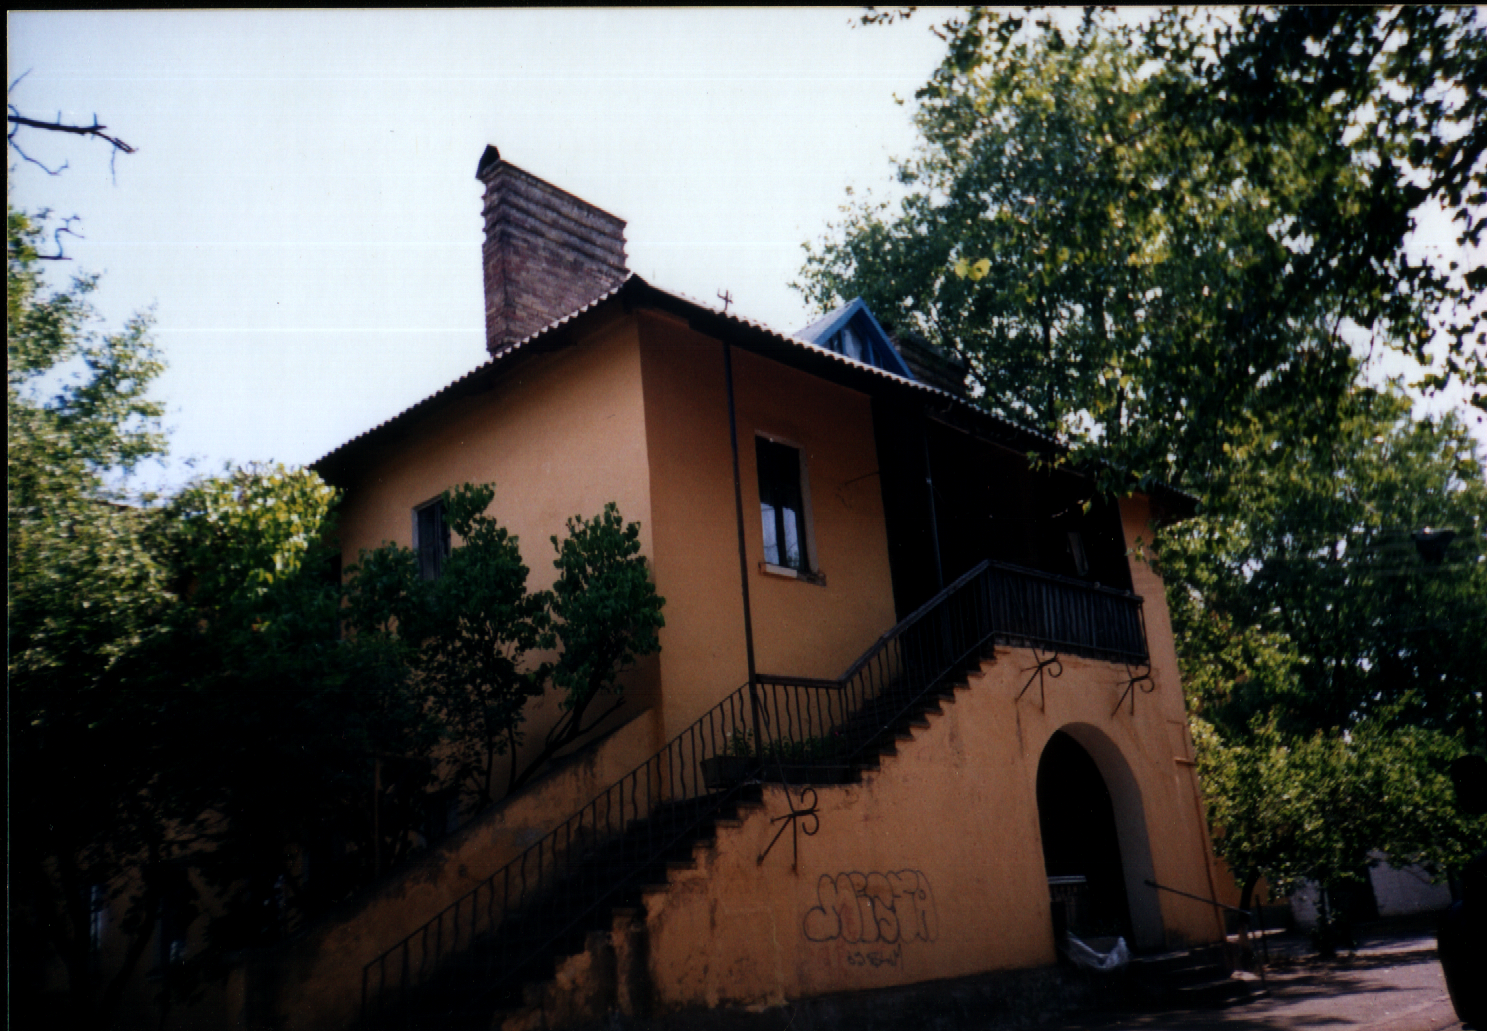
\includegraphics[width=\linewidth]{lpix/out0002.png}

\textit{Аварийный поселок. Угол Красноткацкой. Теперь здесь небоскреб.}
\end{center}

\newpage

\begin{center}
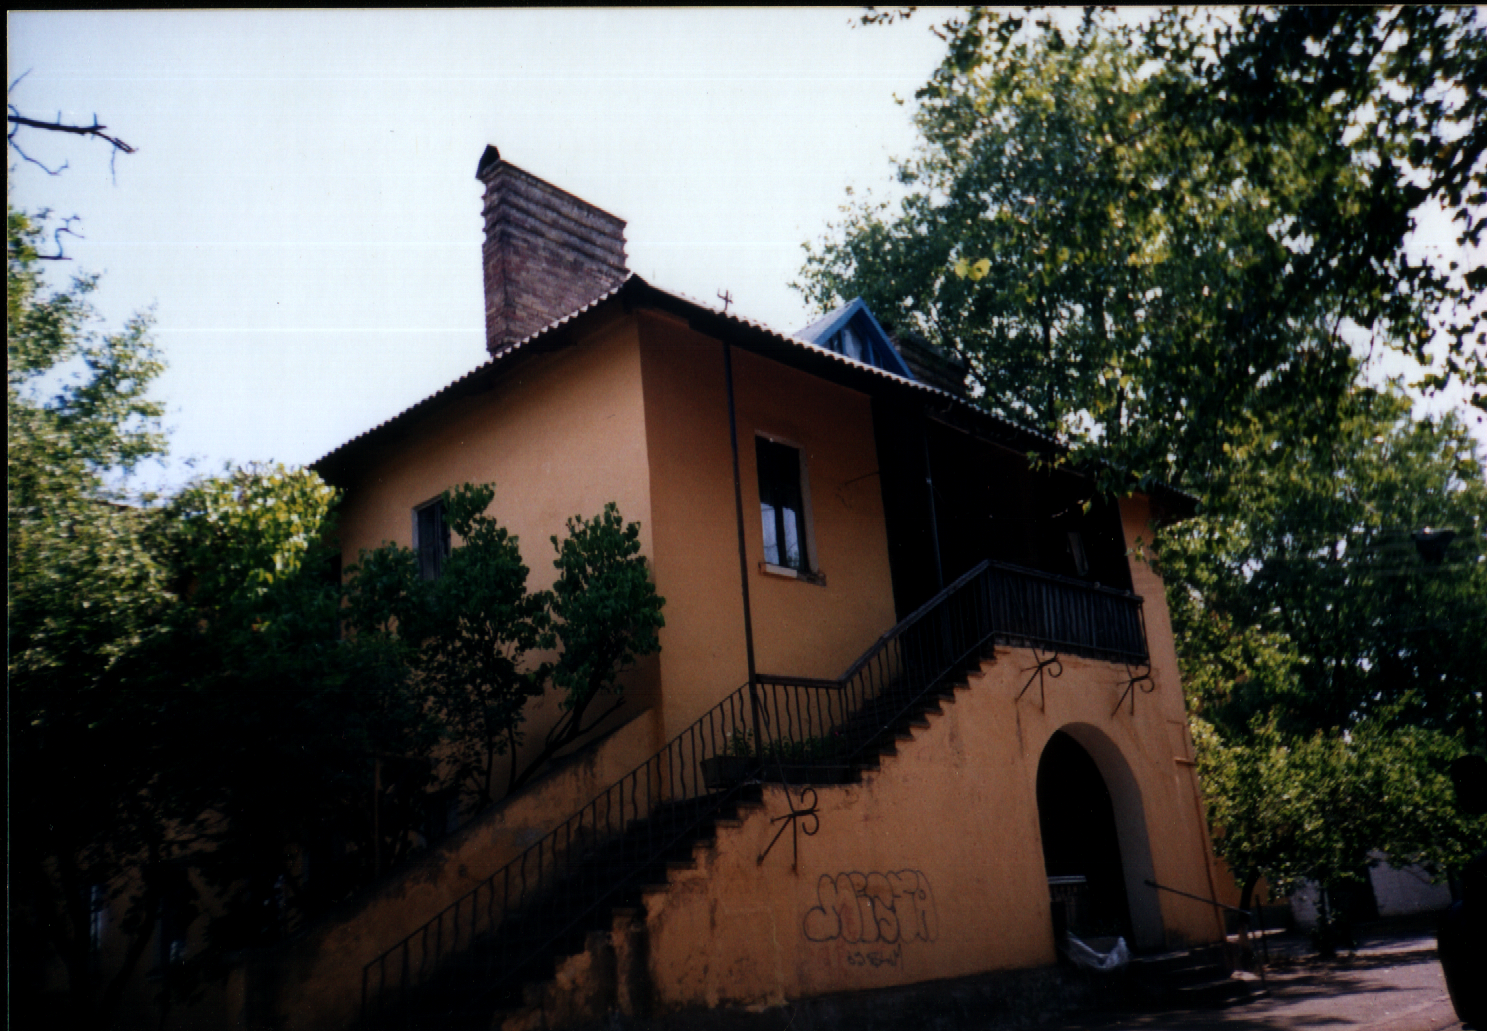
\includegraphics[width=\linewidth]{lpix/out0002.png}

\textit{Аварийный поселок. Угол Красноткацкой. Теперь здесь небоскреб.}
\end{center}

\newpage

\vspace*{\fill}


\begin{center}
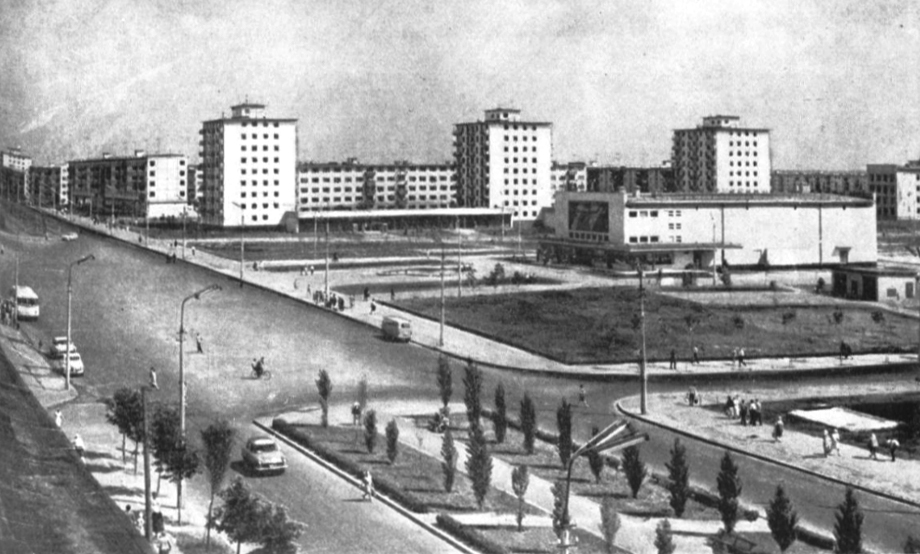
\includegraphics[width=\linewidth]{lpix/avrova-1960x.jpg}

\textit{Кинотеатр "Аврора", конец 1960х -70-е.}
\end{center}

\begin{center}
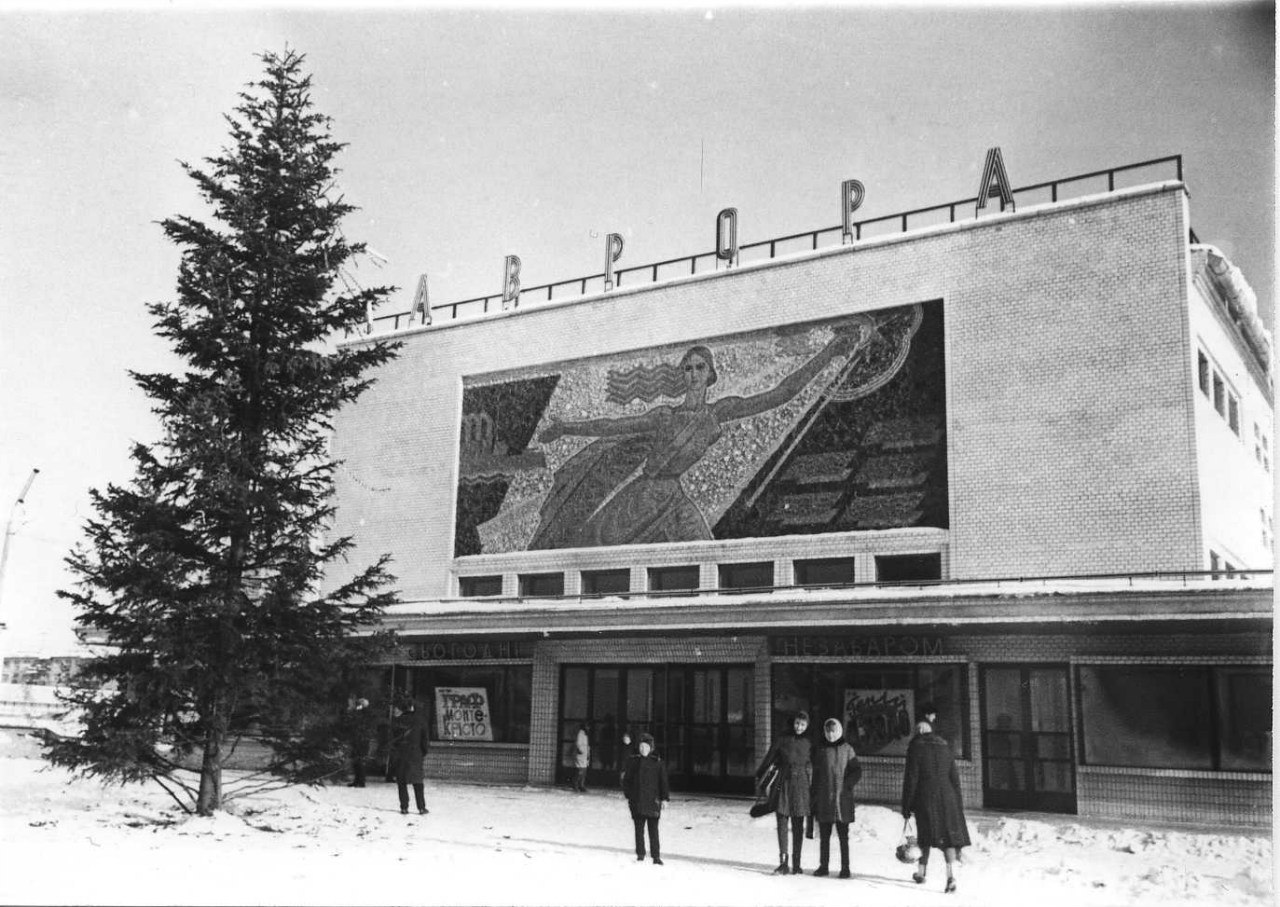
\includegraphics[width=\linewidth]{lpix/avrora-1970-75.jpg}

\textit{Кинотеатр "Аврора", первая половина 1970х.}
\end{center}


\vspace*{\fill}

\newpage


\begin{center}
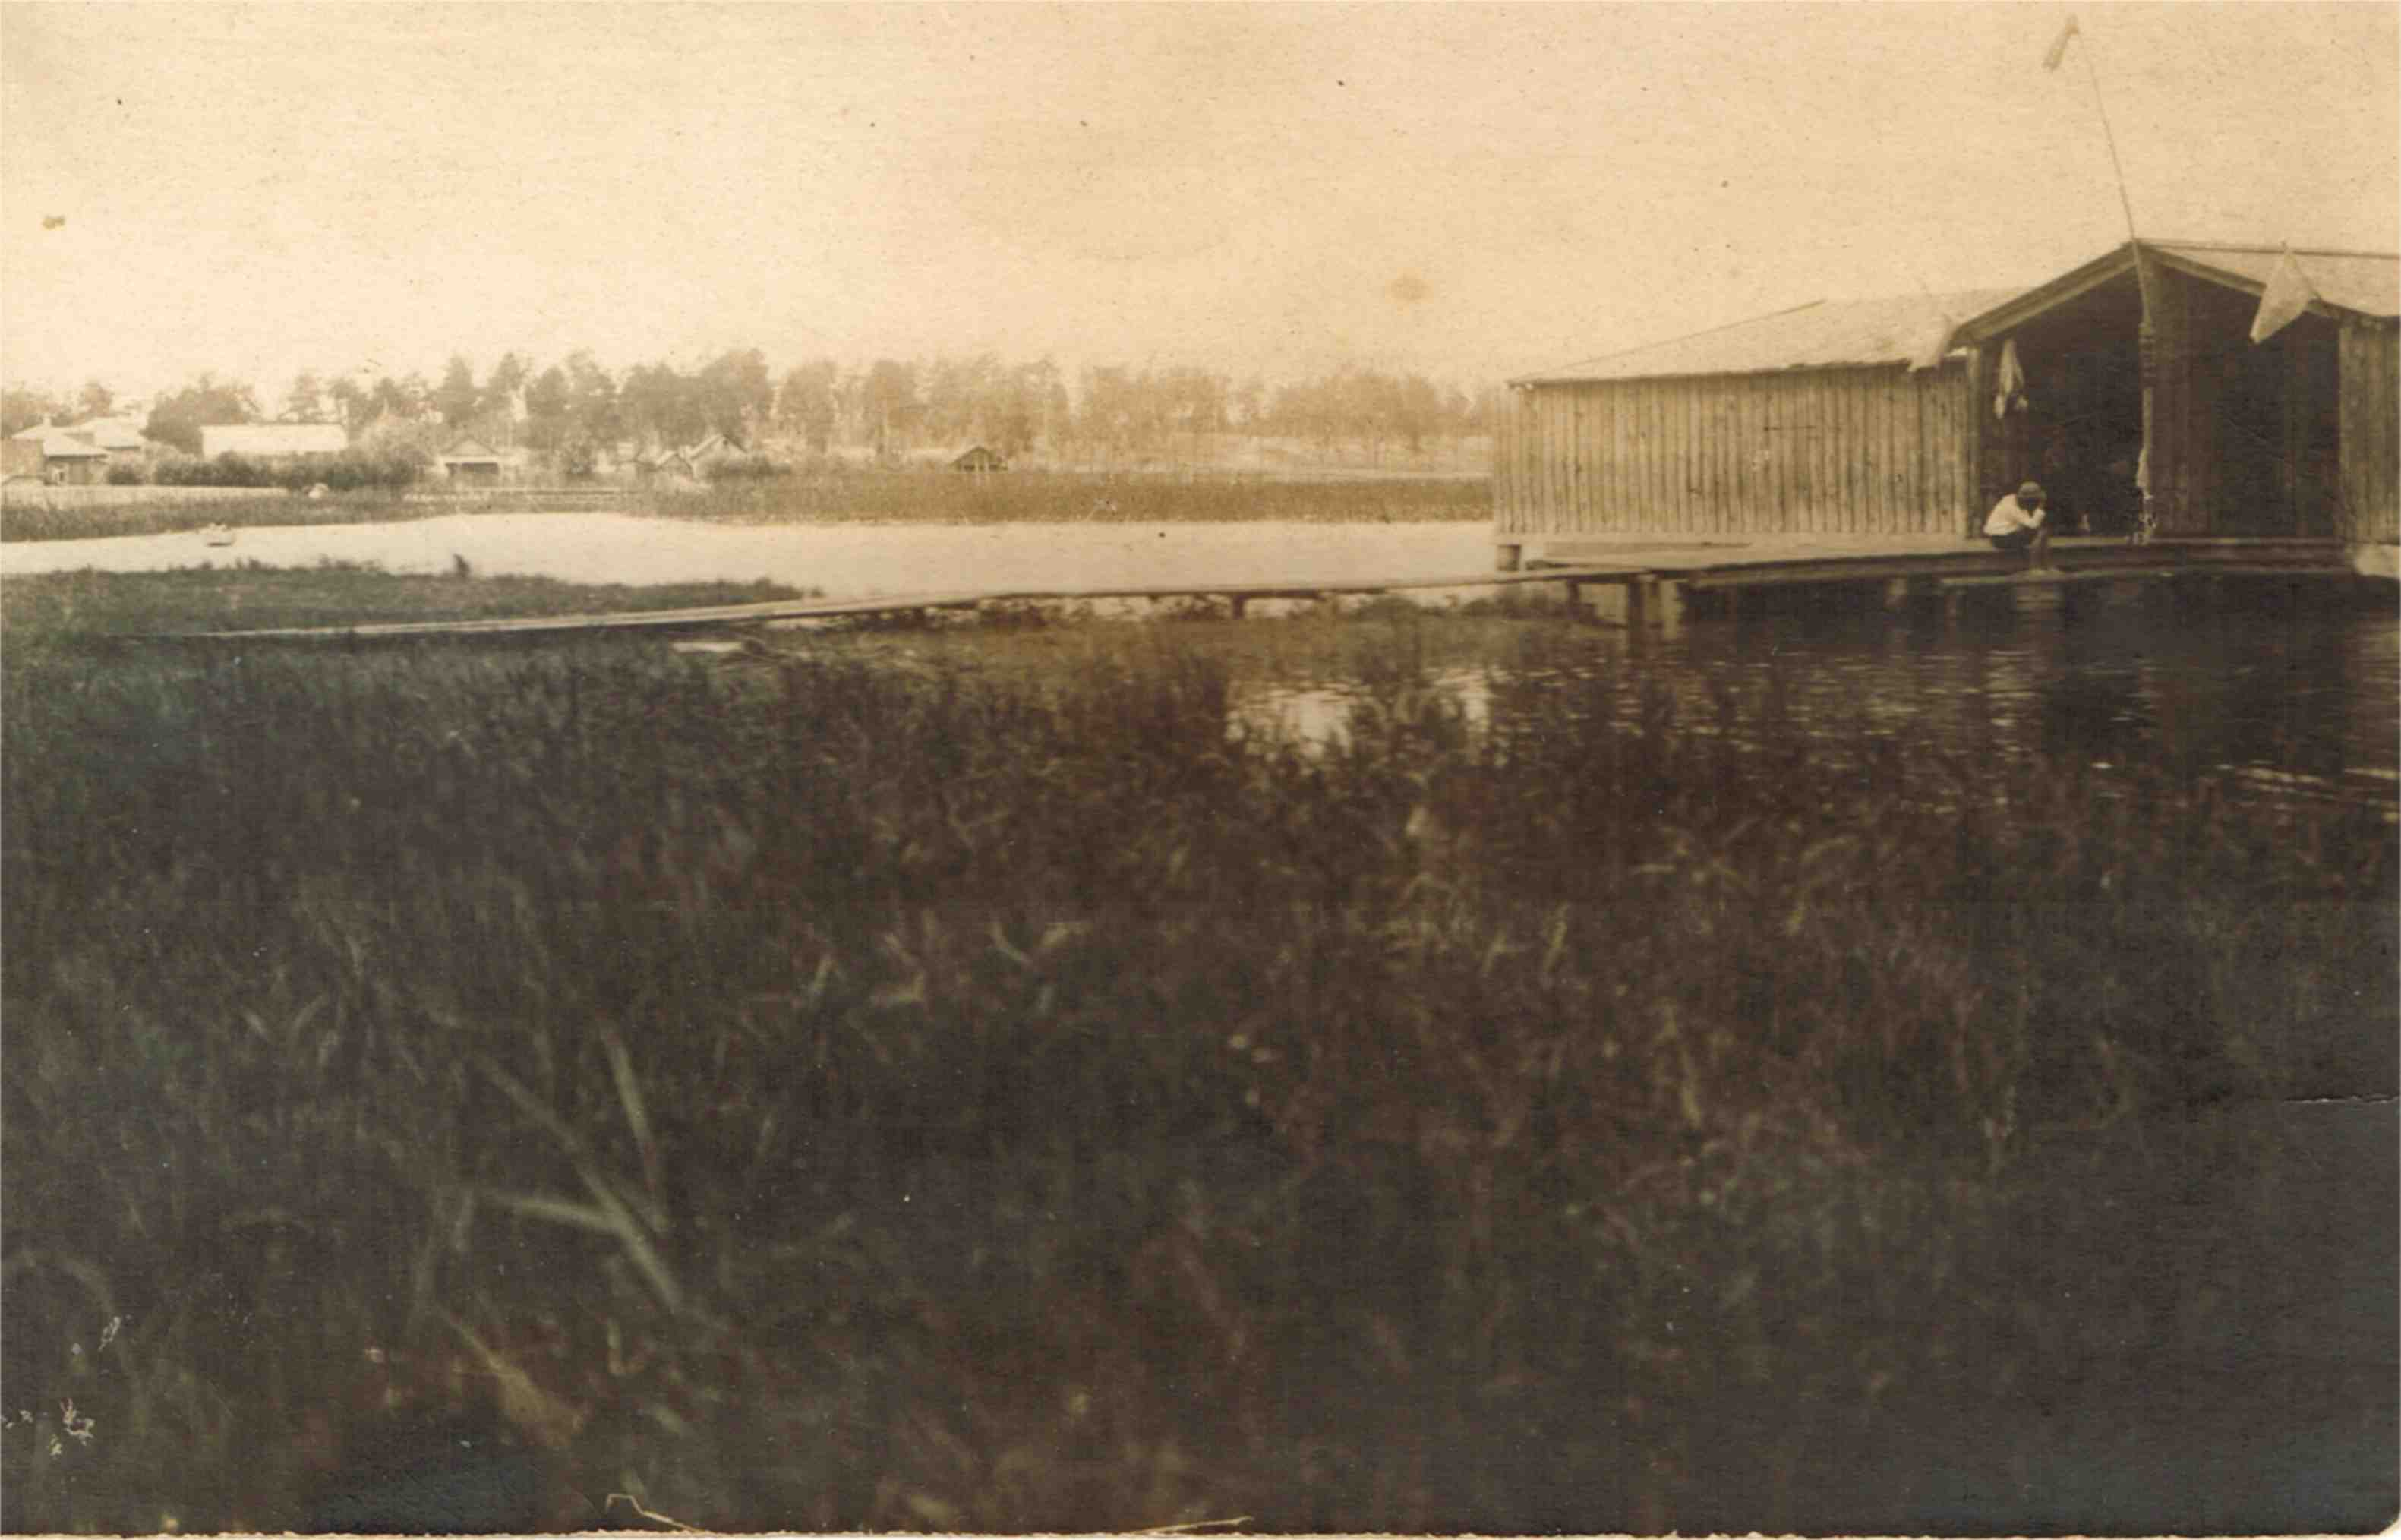
\includegraphics[width=\linewidth]{lpix/darnickoe-ozero-dprev.jpg}

\textit{Дарницкое озеро. Дореволюционный снимокъ.}
\end{center}

\begin{center}
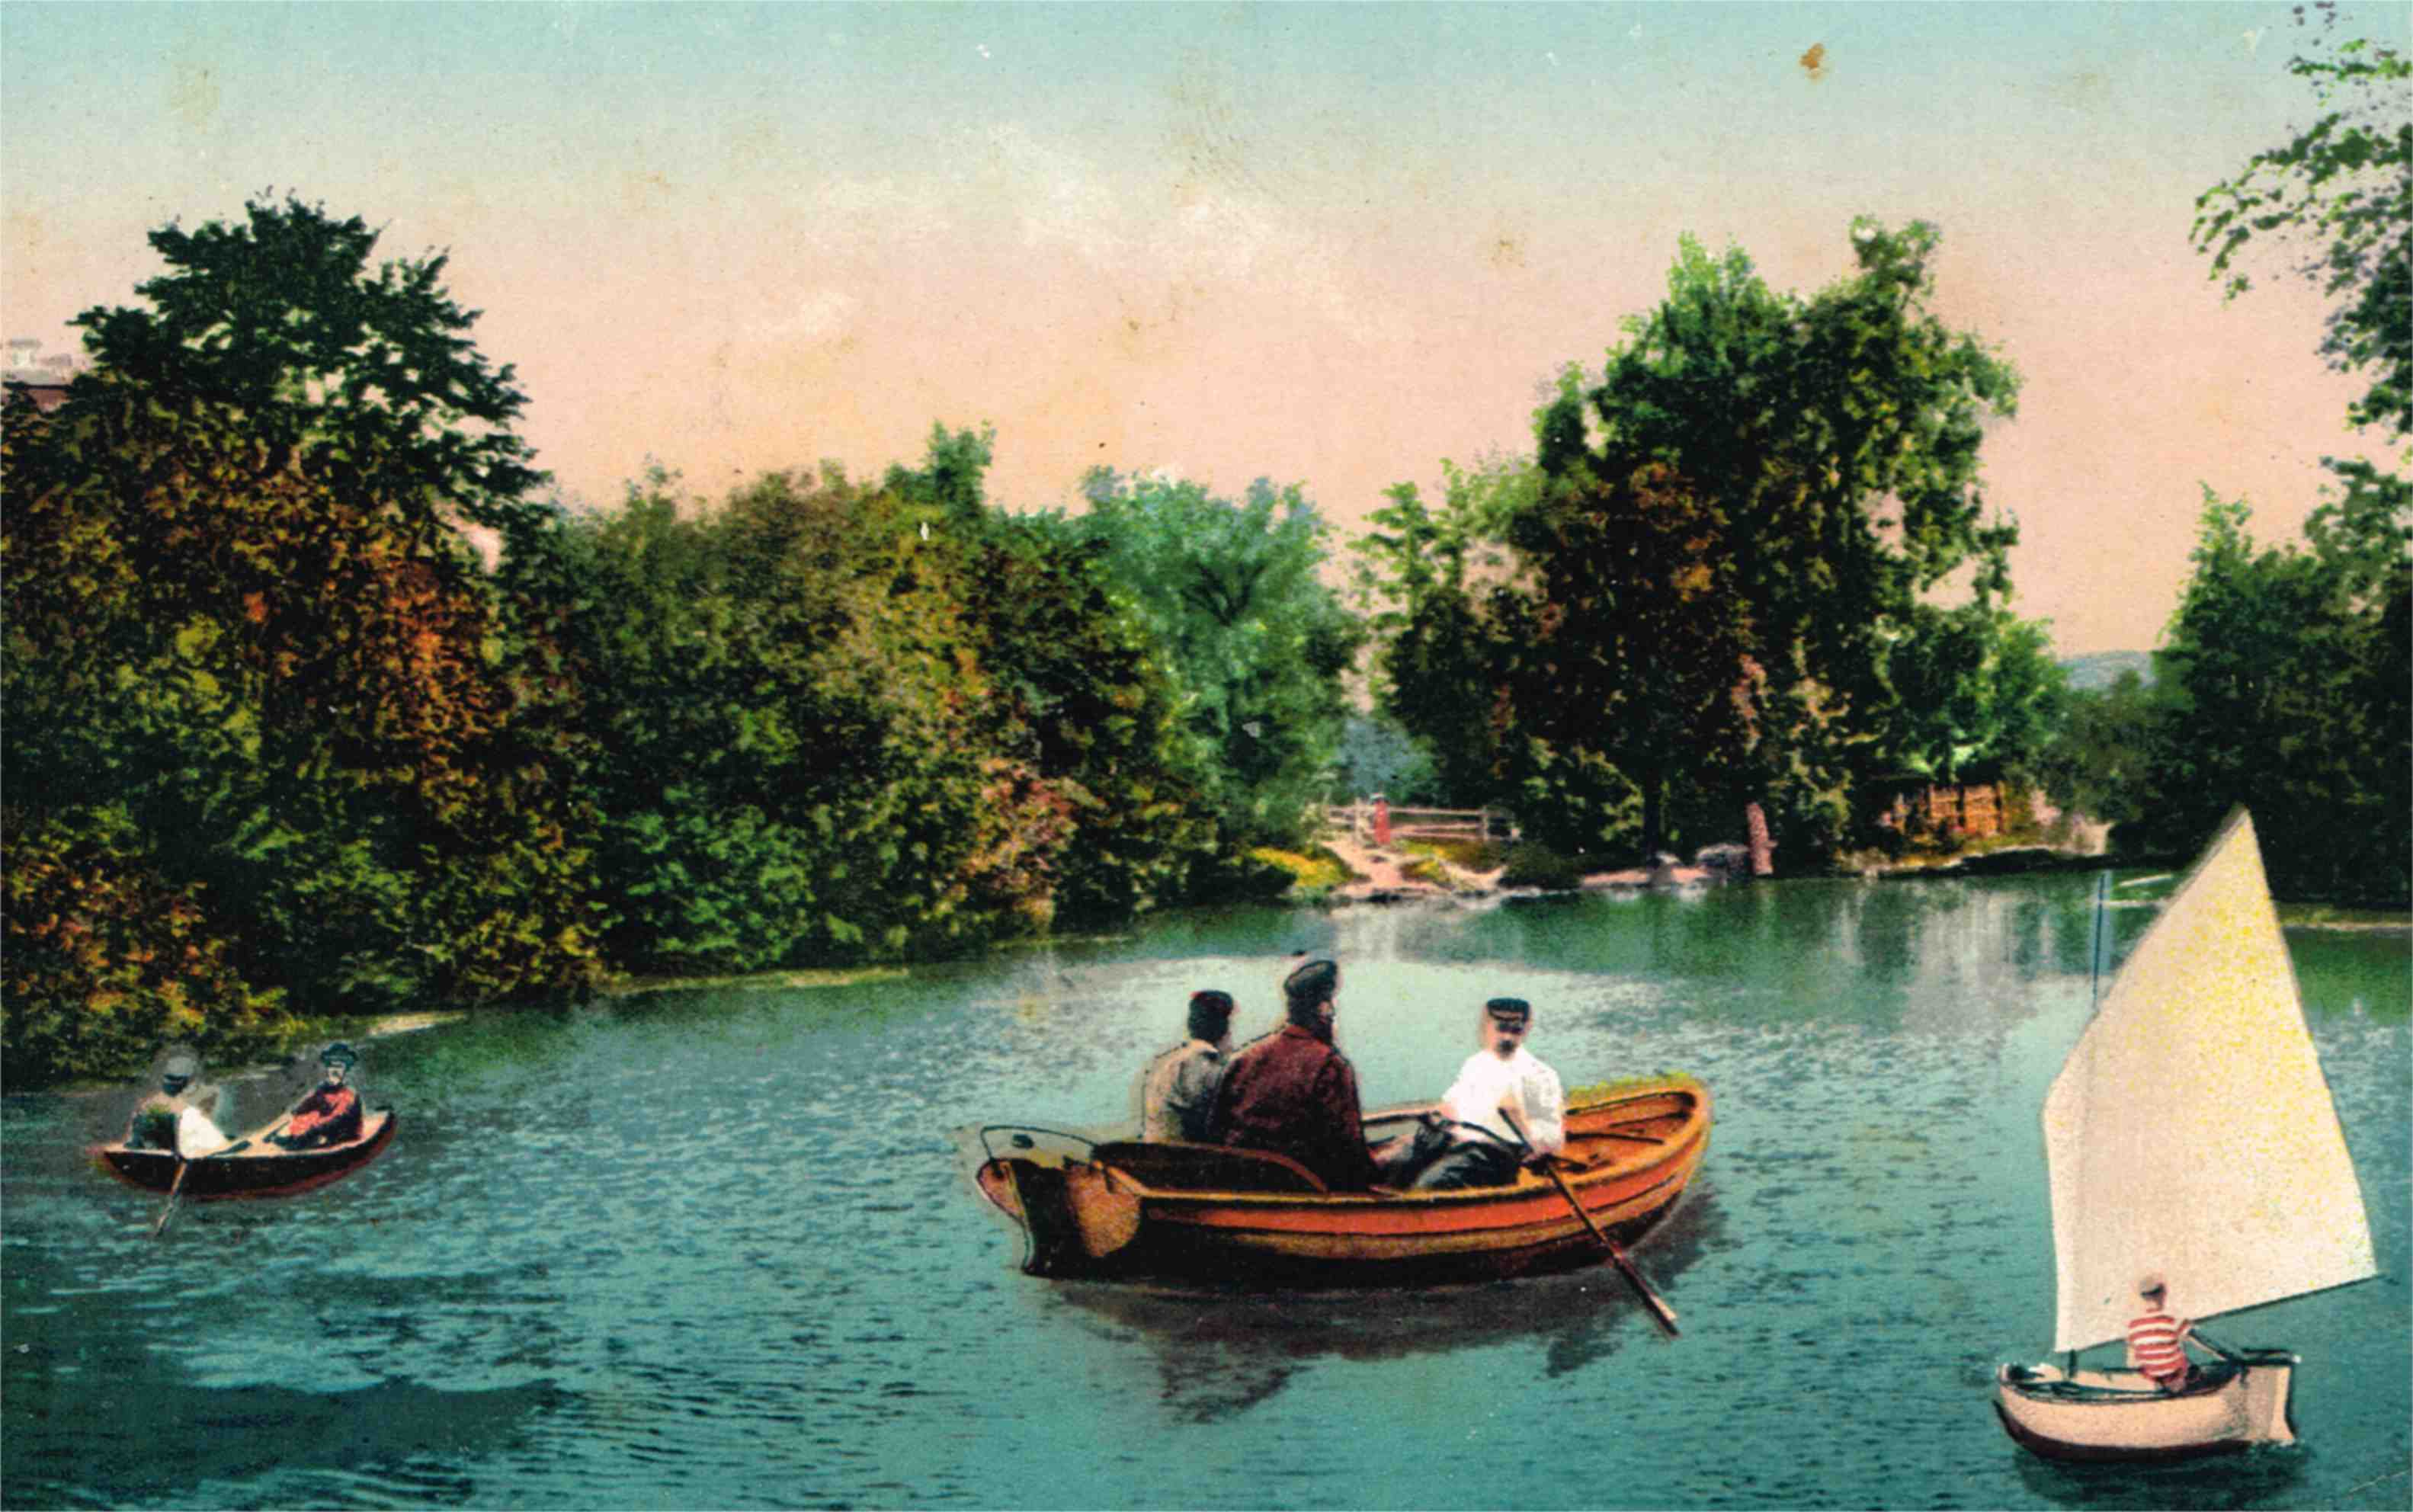
\includegraphics[width=\linewidth]{lpix/darn.jpg}

\textit{Дарницкое озеро. Старинная открытка.}
\end{center}

\vspace*{\fill}

\newpage

\vspace*{\fill}

\begin{center}
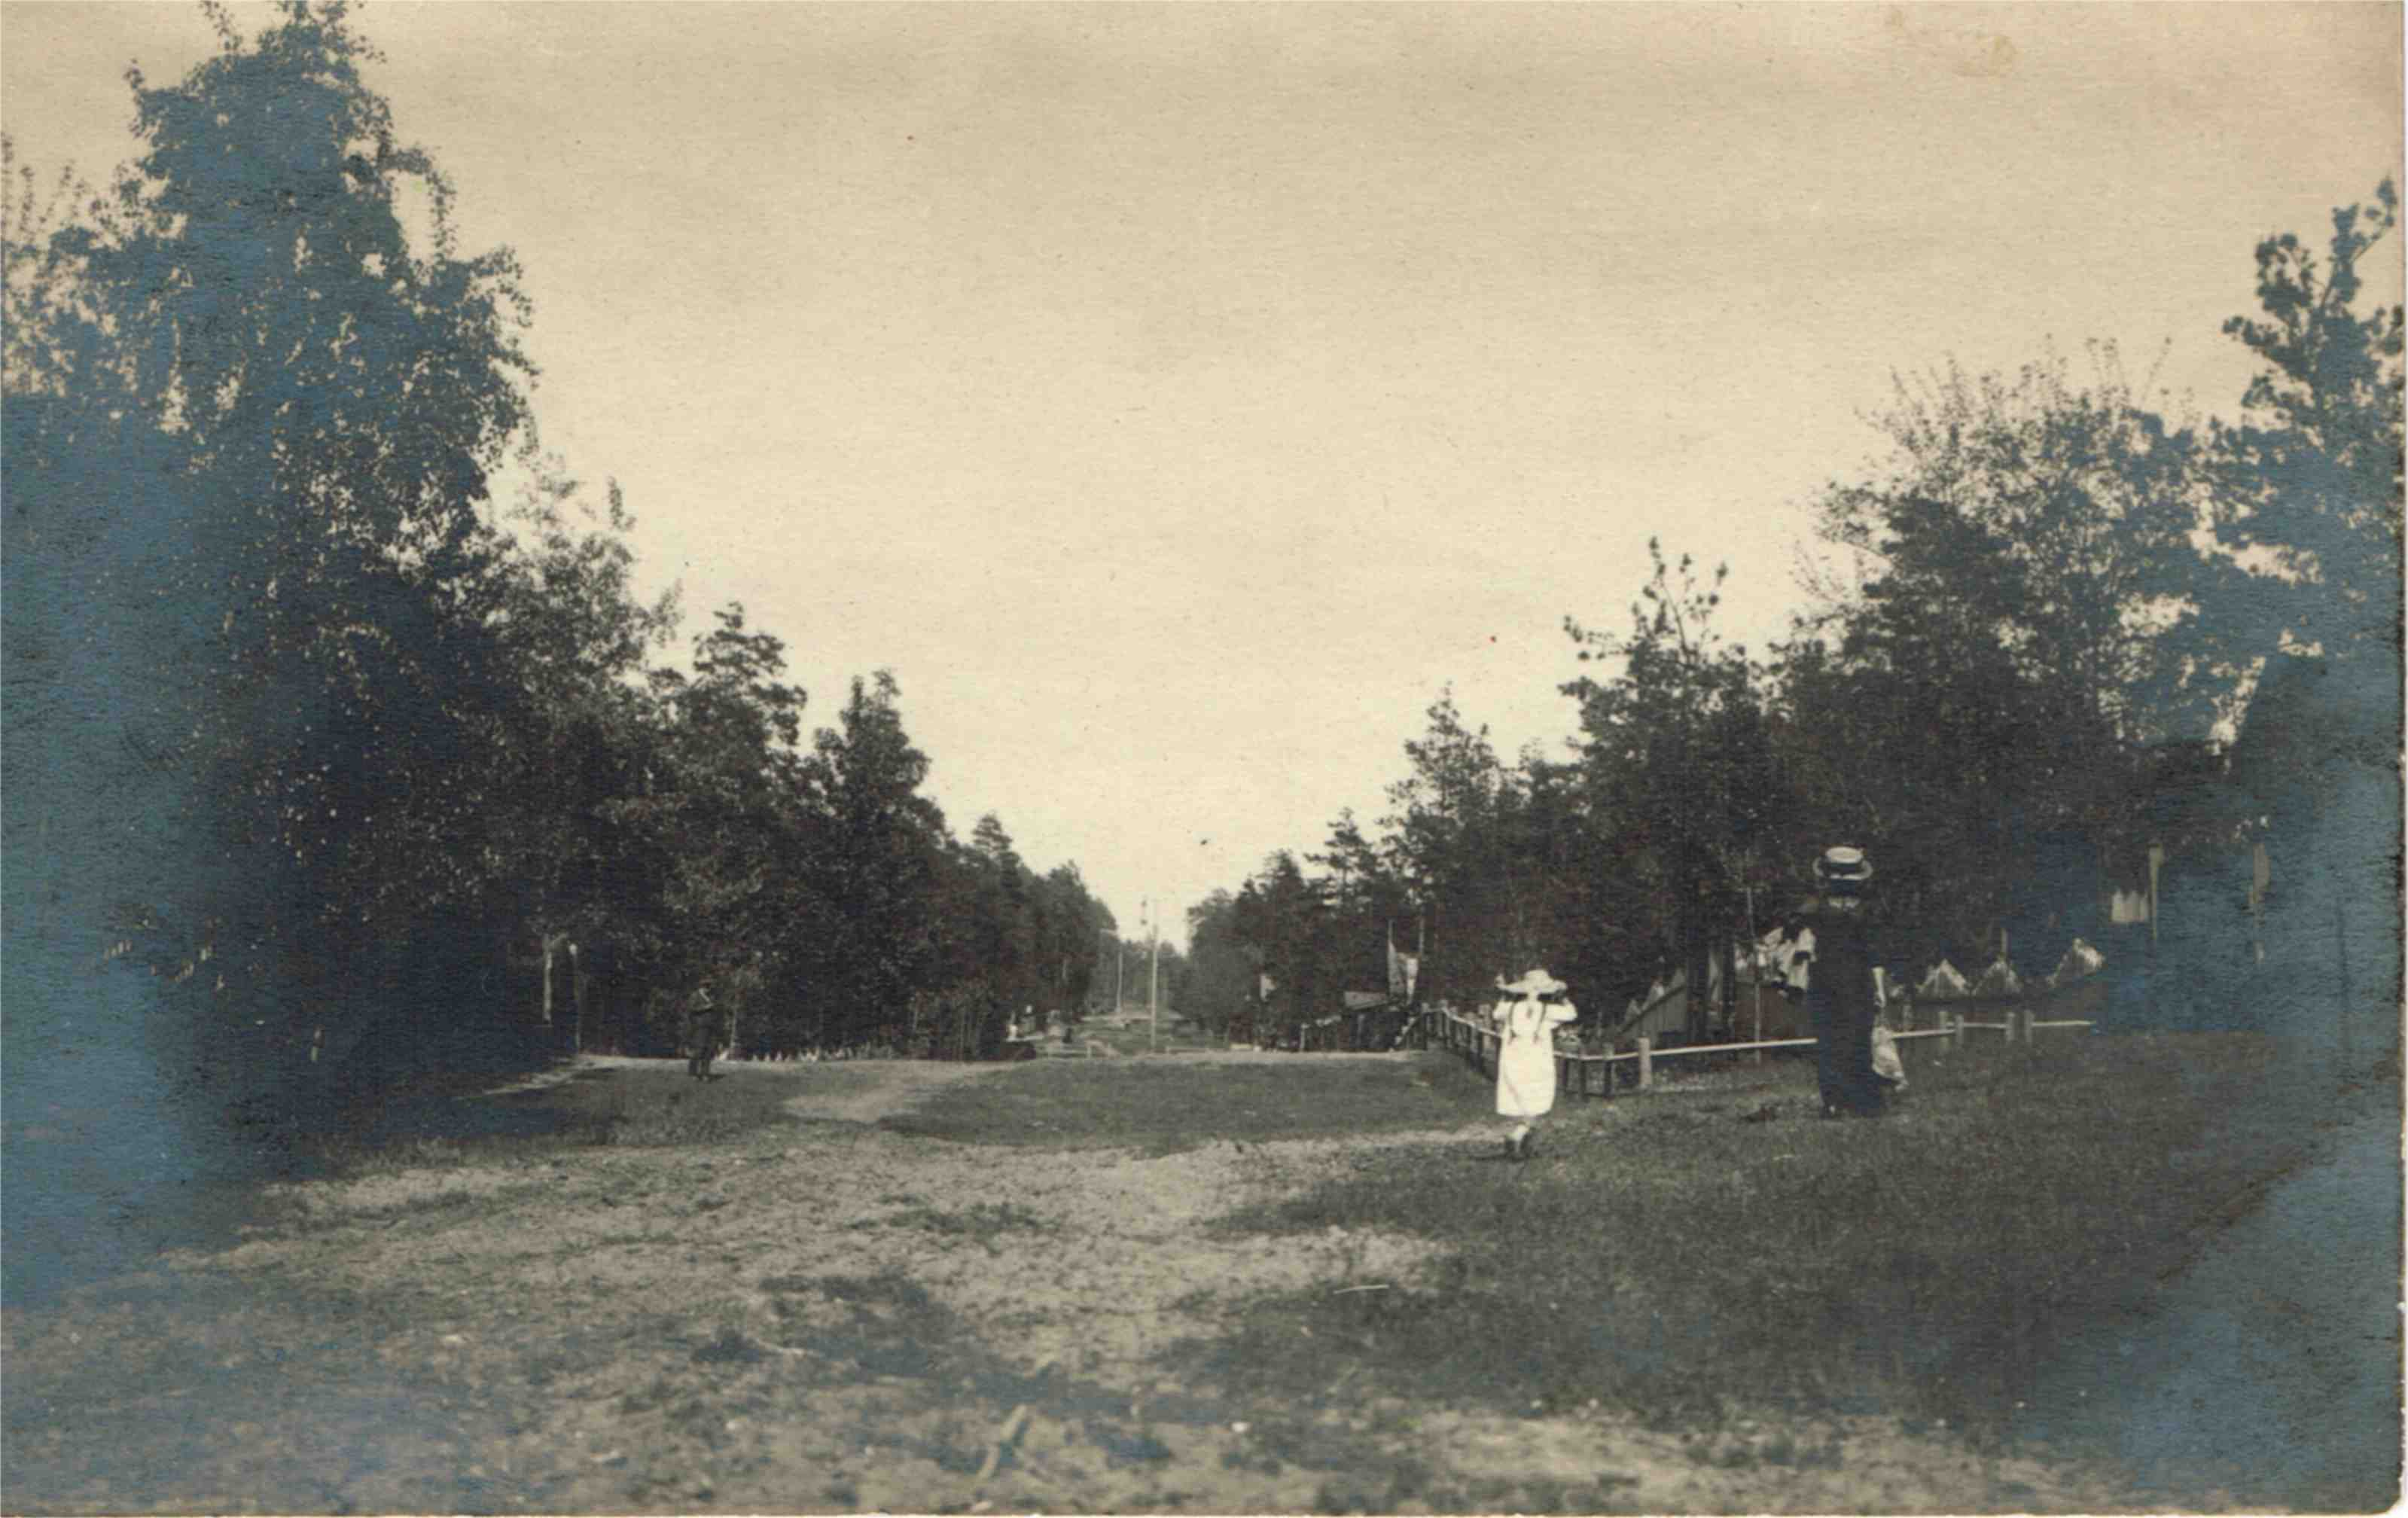
\includegraphics[width=\linewidth]{lpix/darn01.jpg}

\textit{Дарница до революции. Сейчас Старая Дарница.}
\end{center}


\begin{center}
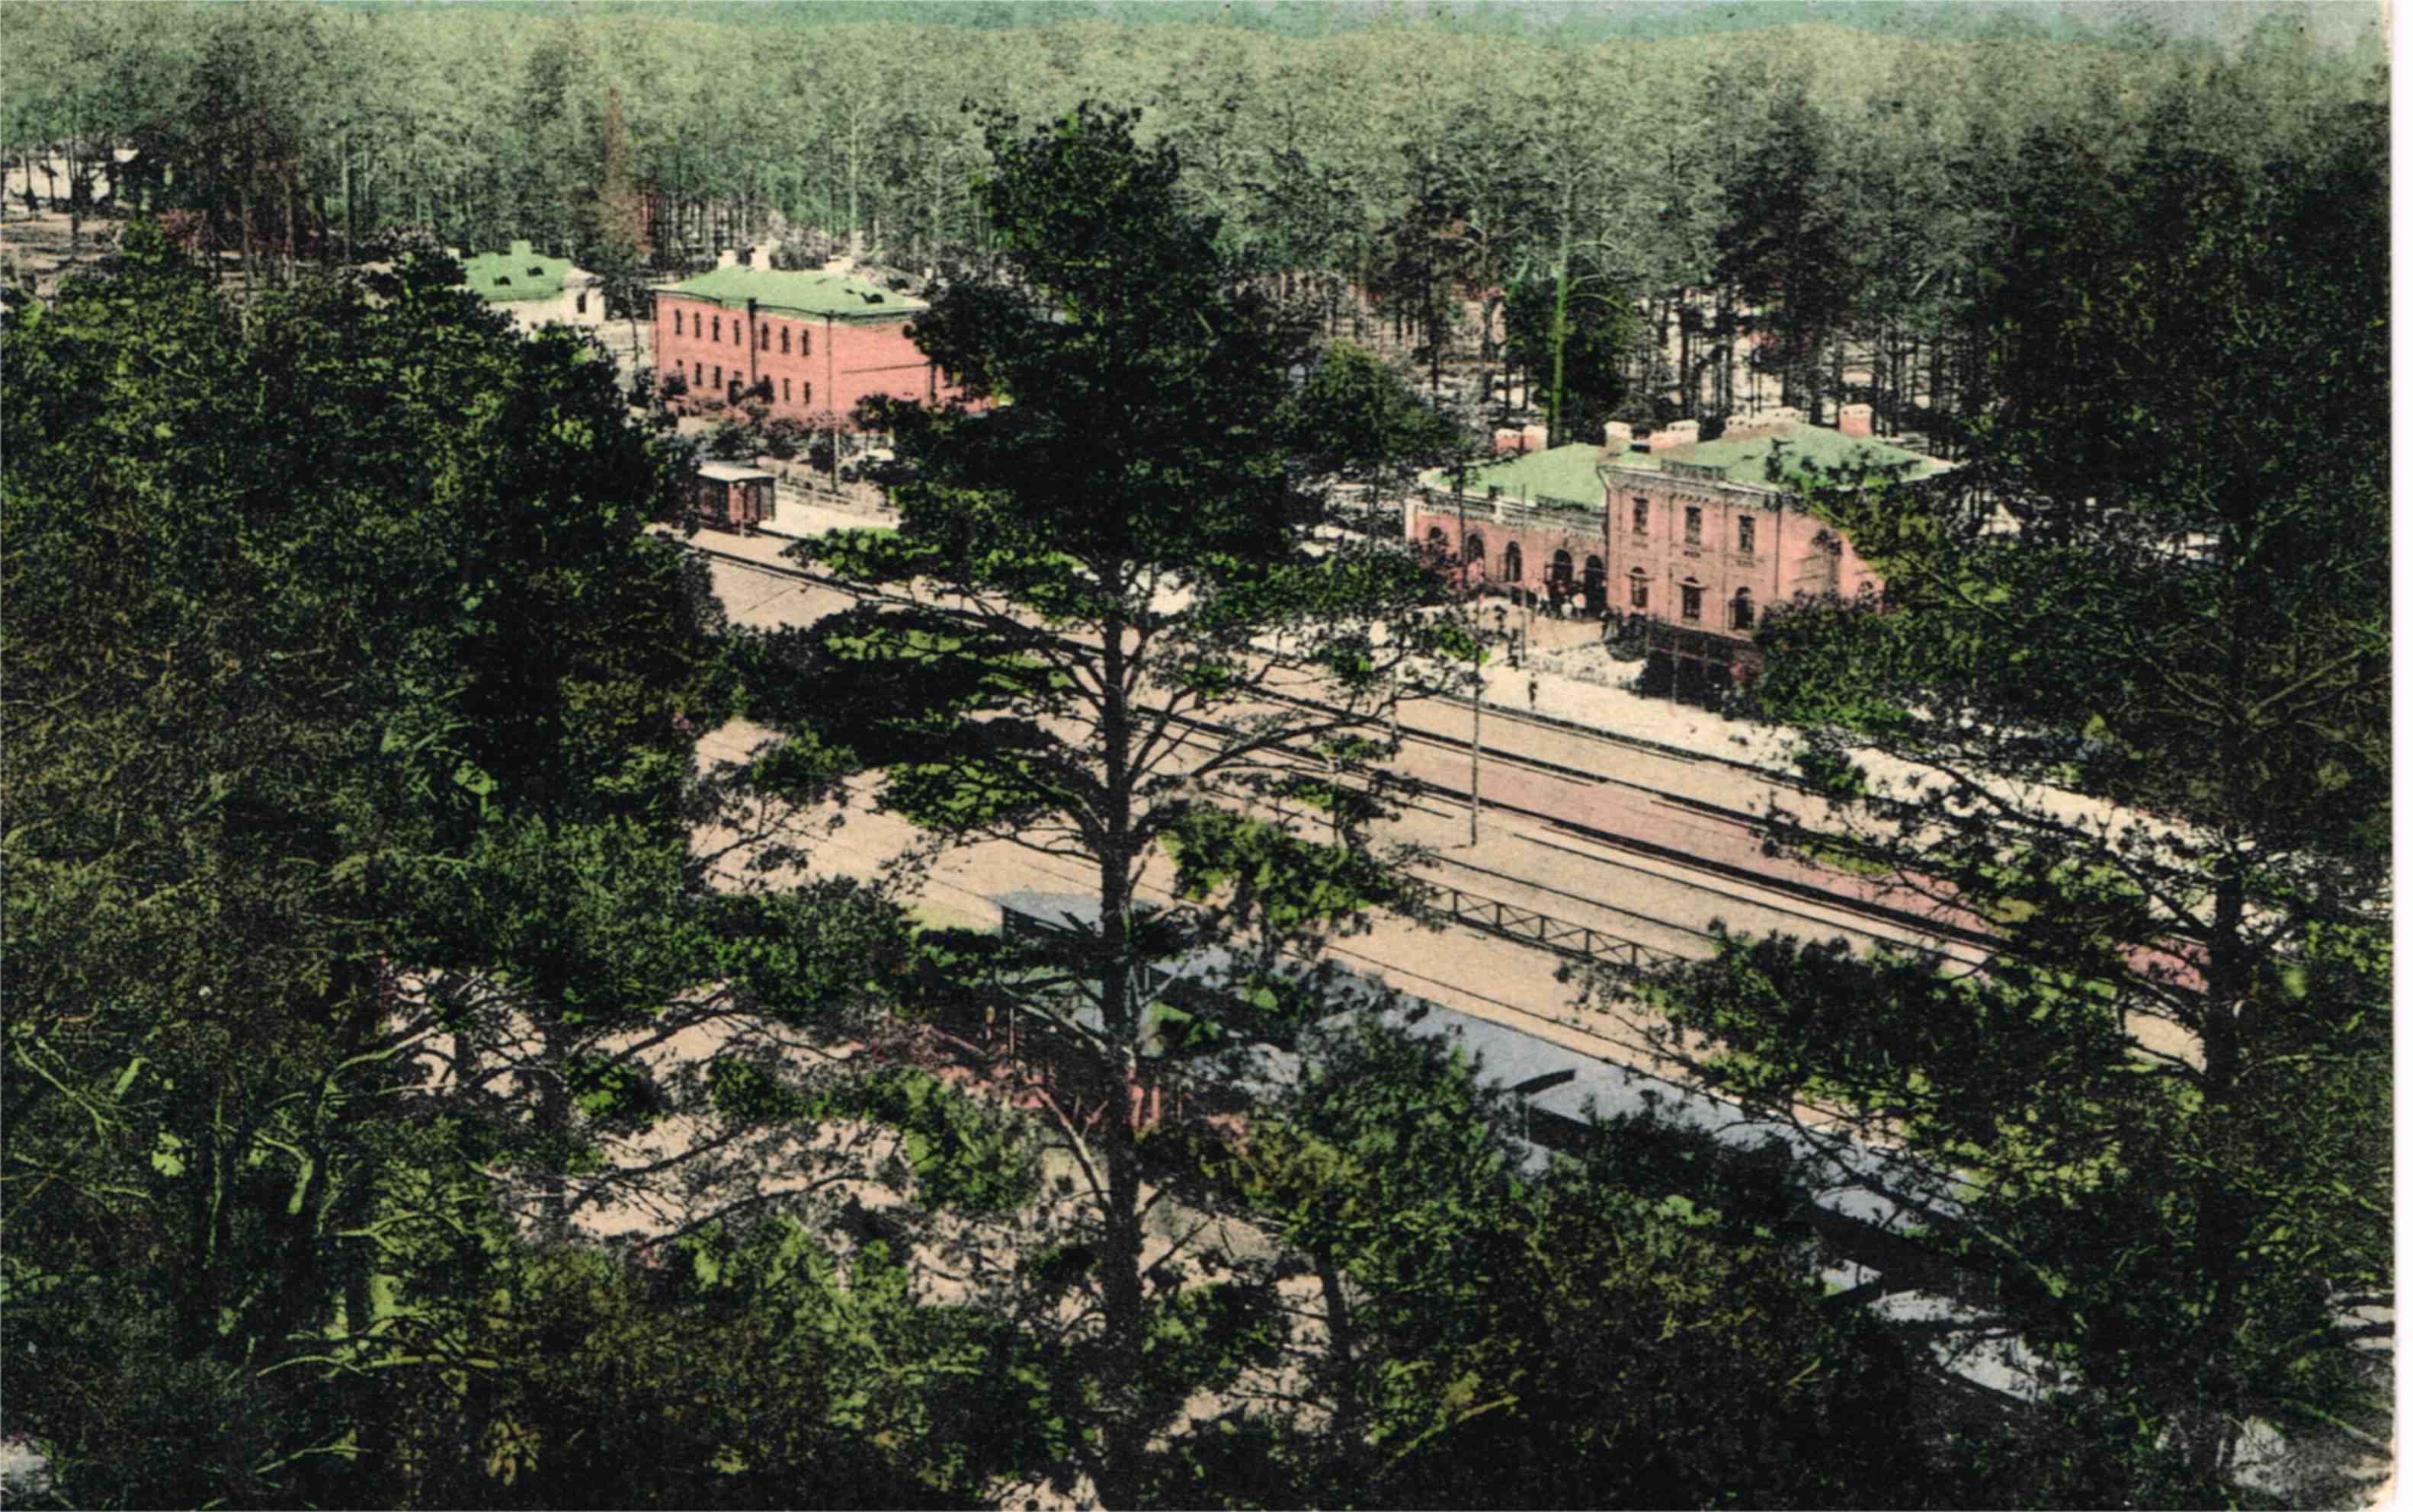
\includegraphics[width=\linewidth]{lpix/darn02.jpg}

\textit{Дарница до революции. Вид на вокзал.}
\end{center}

\vspace*{\fill}

\newpage

\vspace*{\fill}

\begin{center}
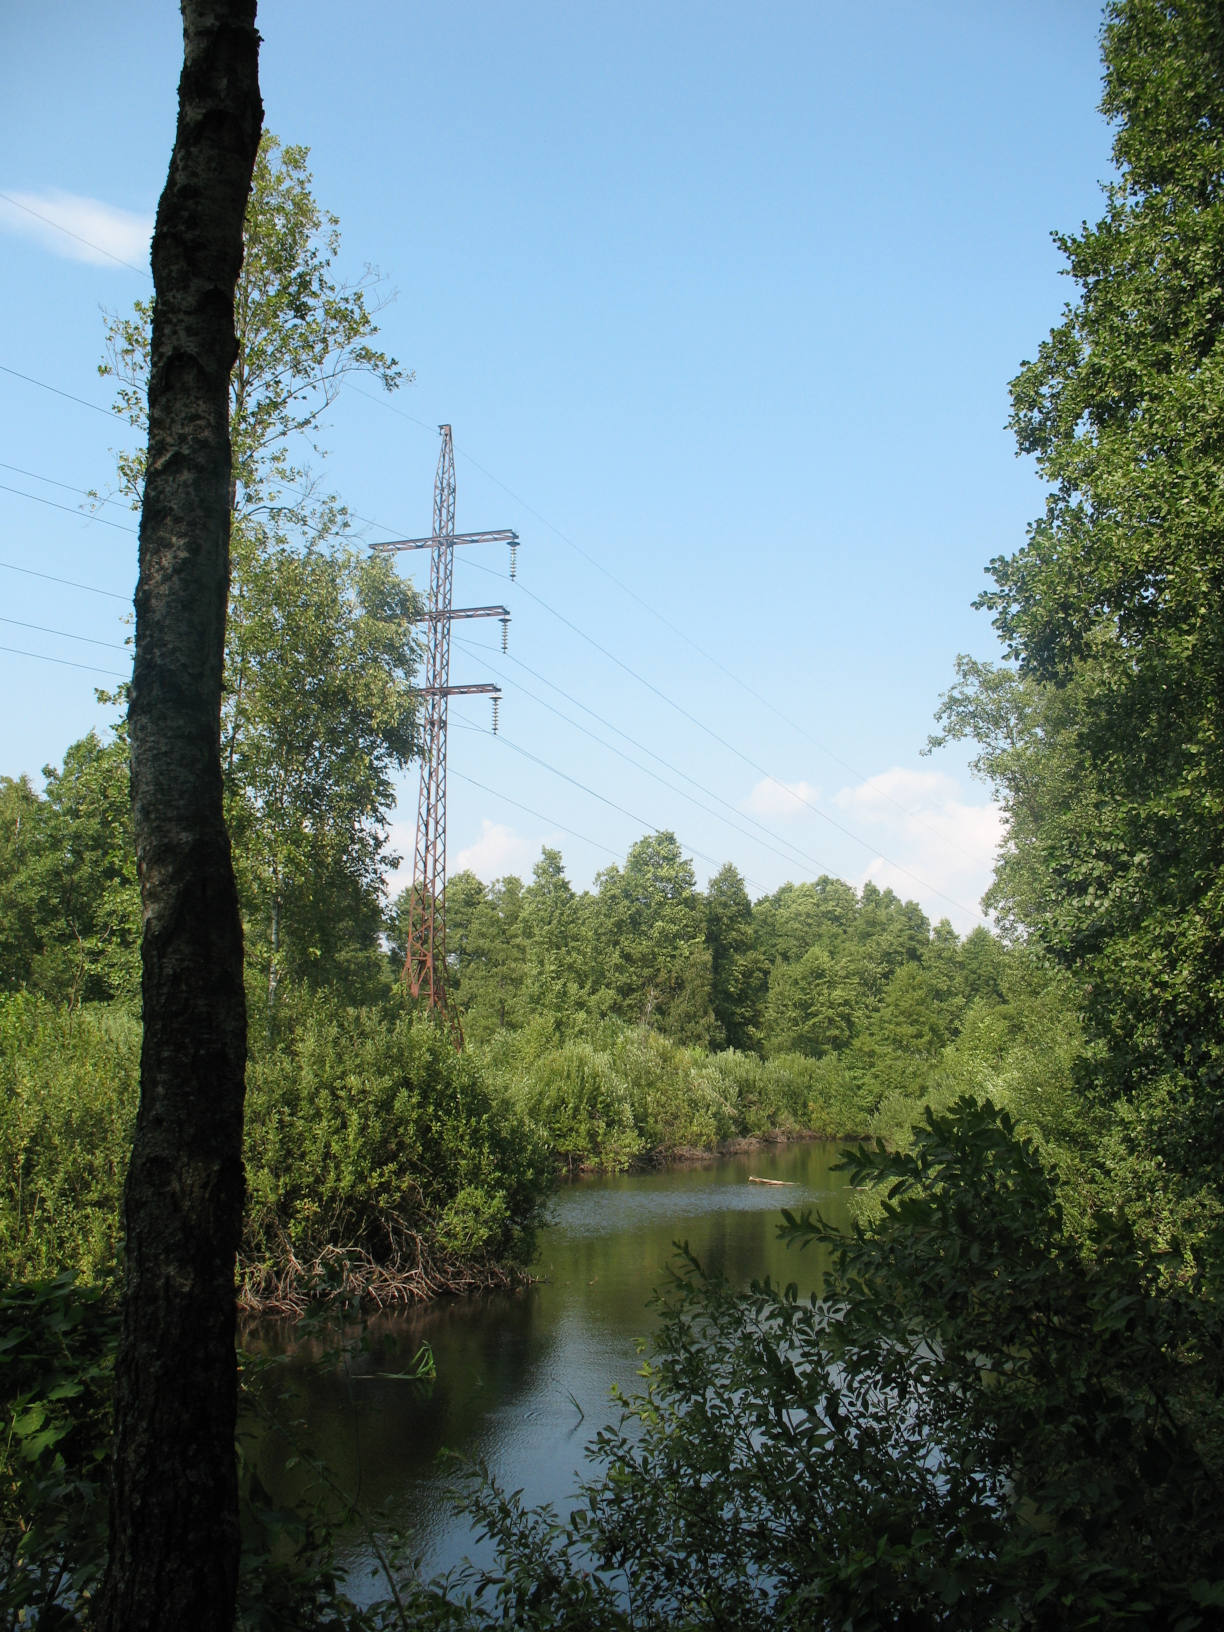
\includegraphics[width=\linewidth]{lpix/darn-reka.jpg}

\textit{Речка Дарница в течении выше озера Березки. 2013.}
\end{center}

\vspace*{\fill}

\newpage

\begin{center}
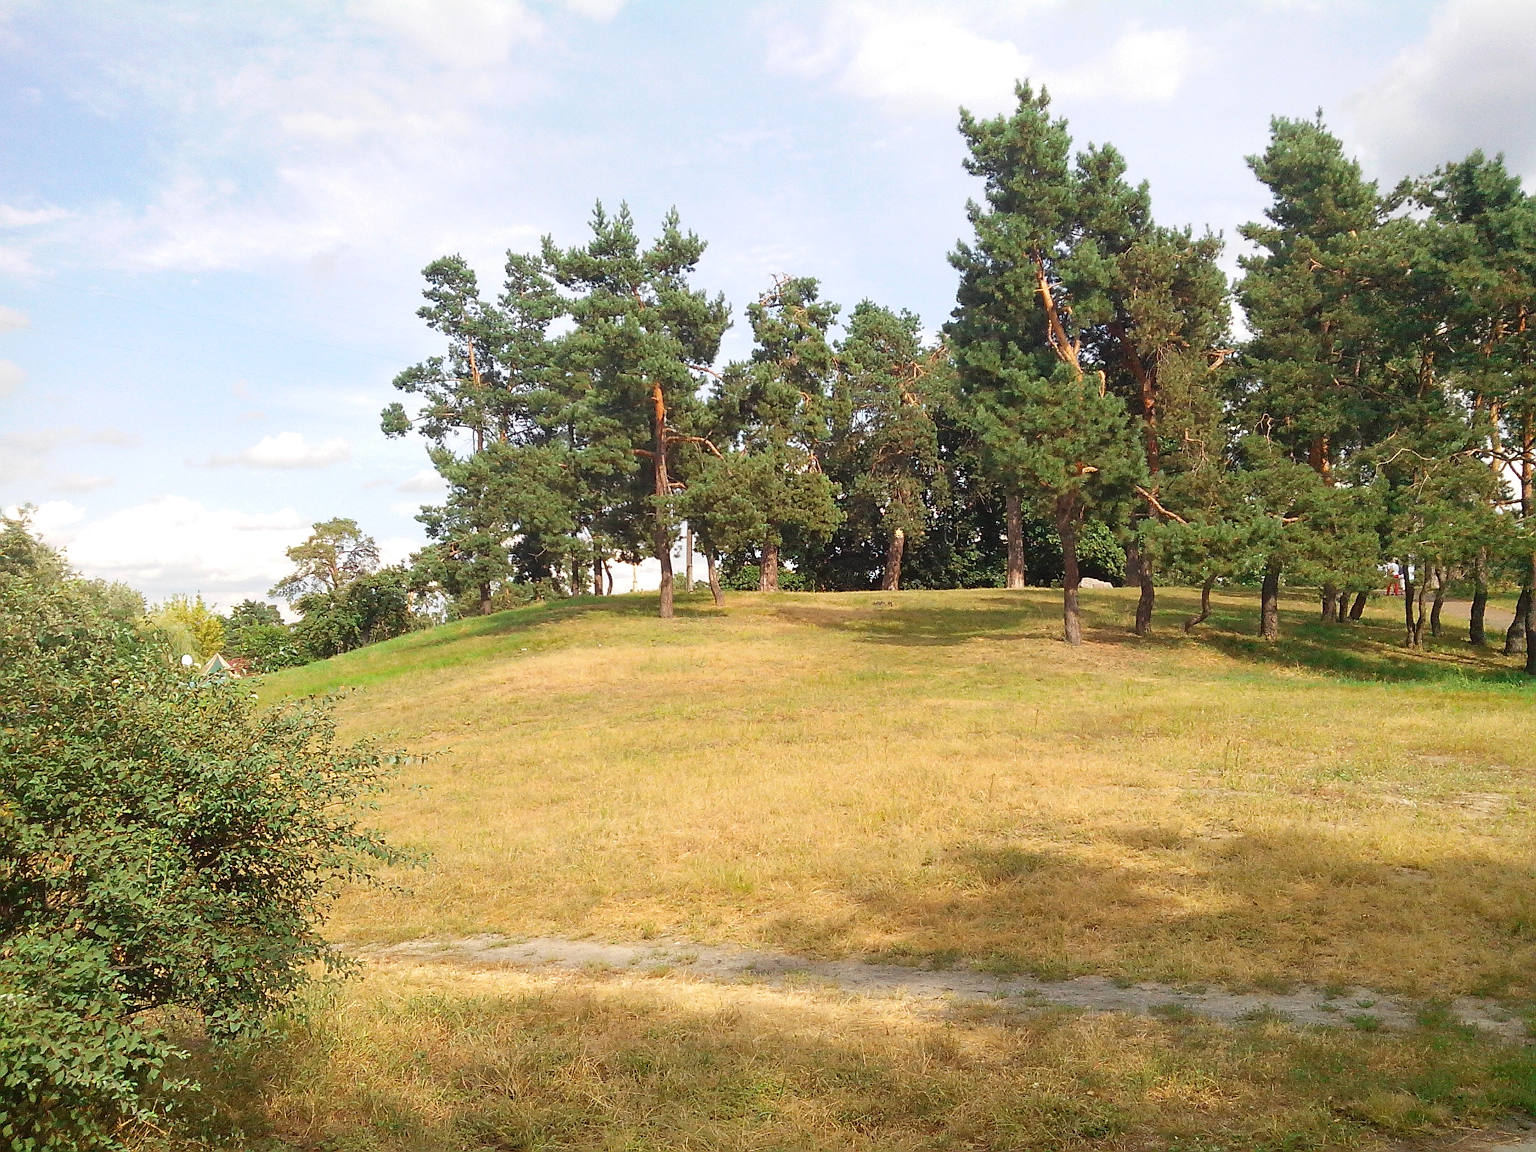
\includegraphics[width=0.95\linewidth]{lpix/IMG_20140817_161555.jpg}

\textit{Волчья гора.}
\end{center}

\begin{center}
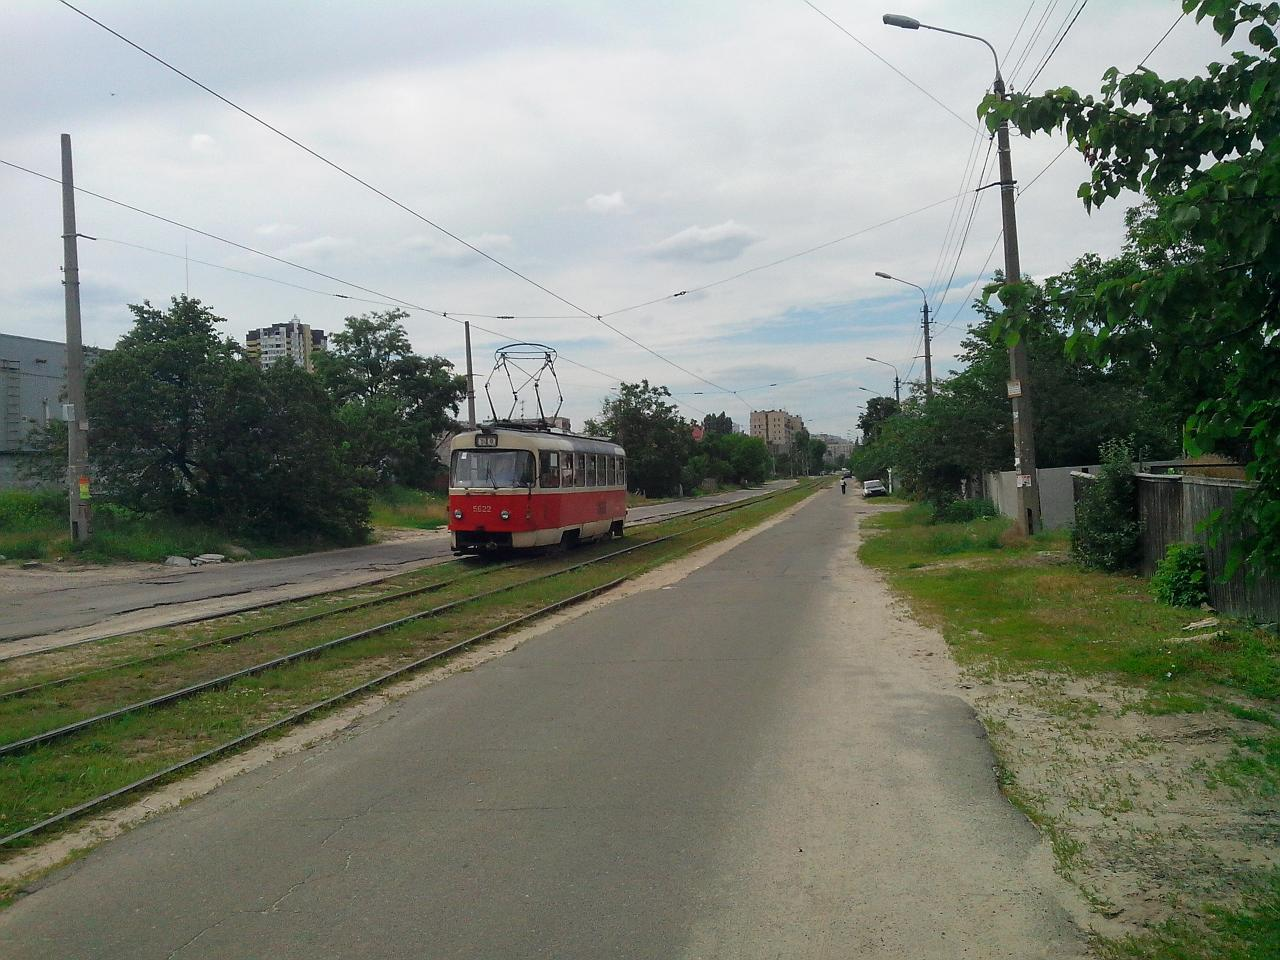
\includegraphics[width=\linewidth]{lpix/IMG_20160613_152358.jpg}

\textit{Красный хутор.}
\end{center}

\newpage

\begin{center}
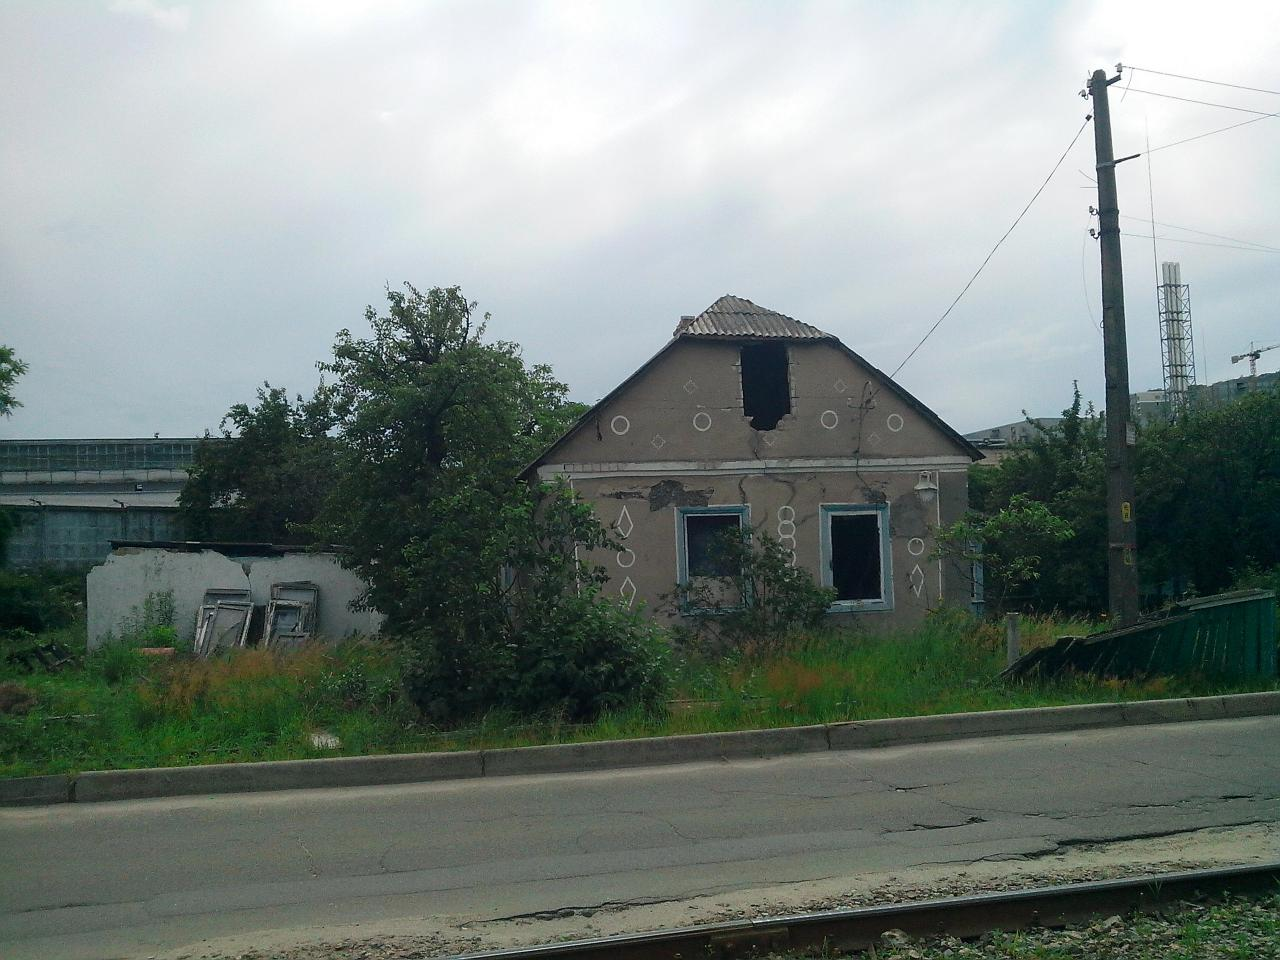
\includegraphics[width=\linewidth]{lpix/IMG_20160613_152456.jpg}

\textit{Красный хутор.}
\end{center}


\begin{center}
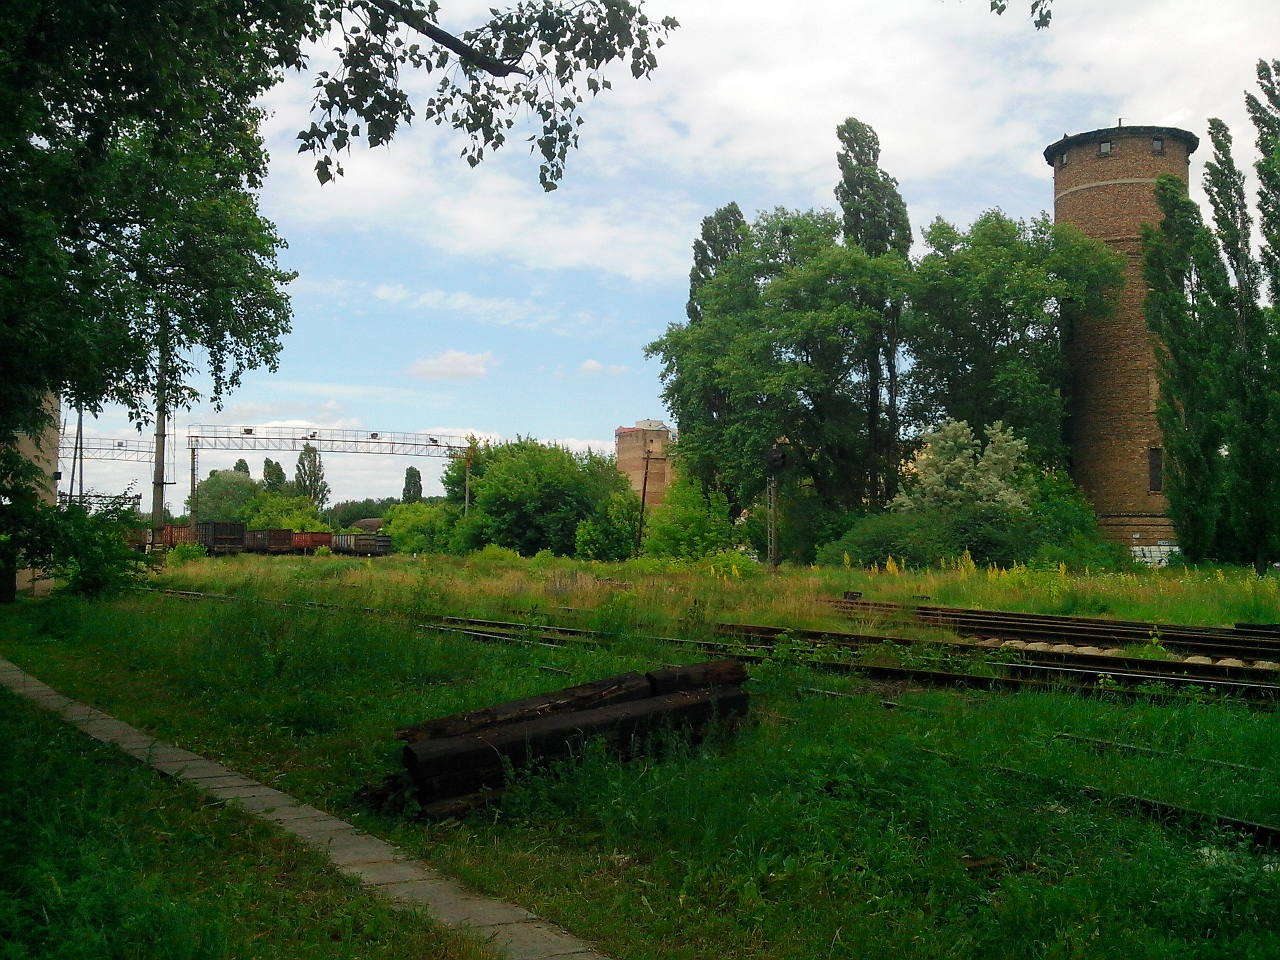
\includegraphics[width=0.95\linewidth]{lpix/IMG_20160613_134918.jpg}

\textit{Лиски, граница с началом ДВРЗ, довоенная водонапорная башня.}
\end{center}



\begin{center}
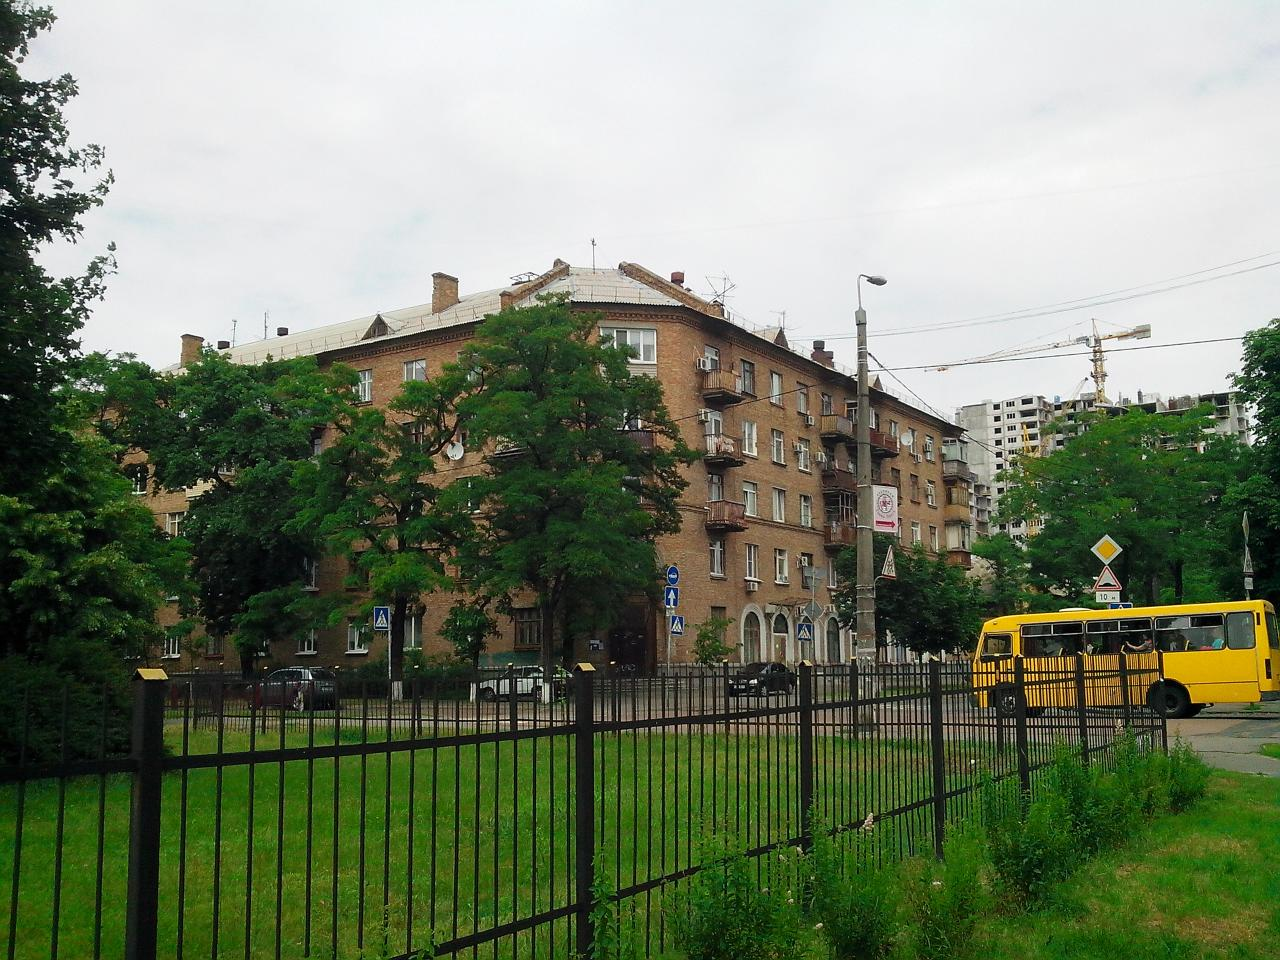
\includegraphics[width=\linewidth]{lpix/IMG_20160613_143111.jpg}

\textit{Новая Дарница.}
\end{center}


\begin{center}
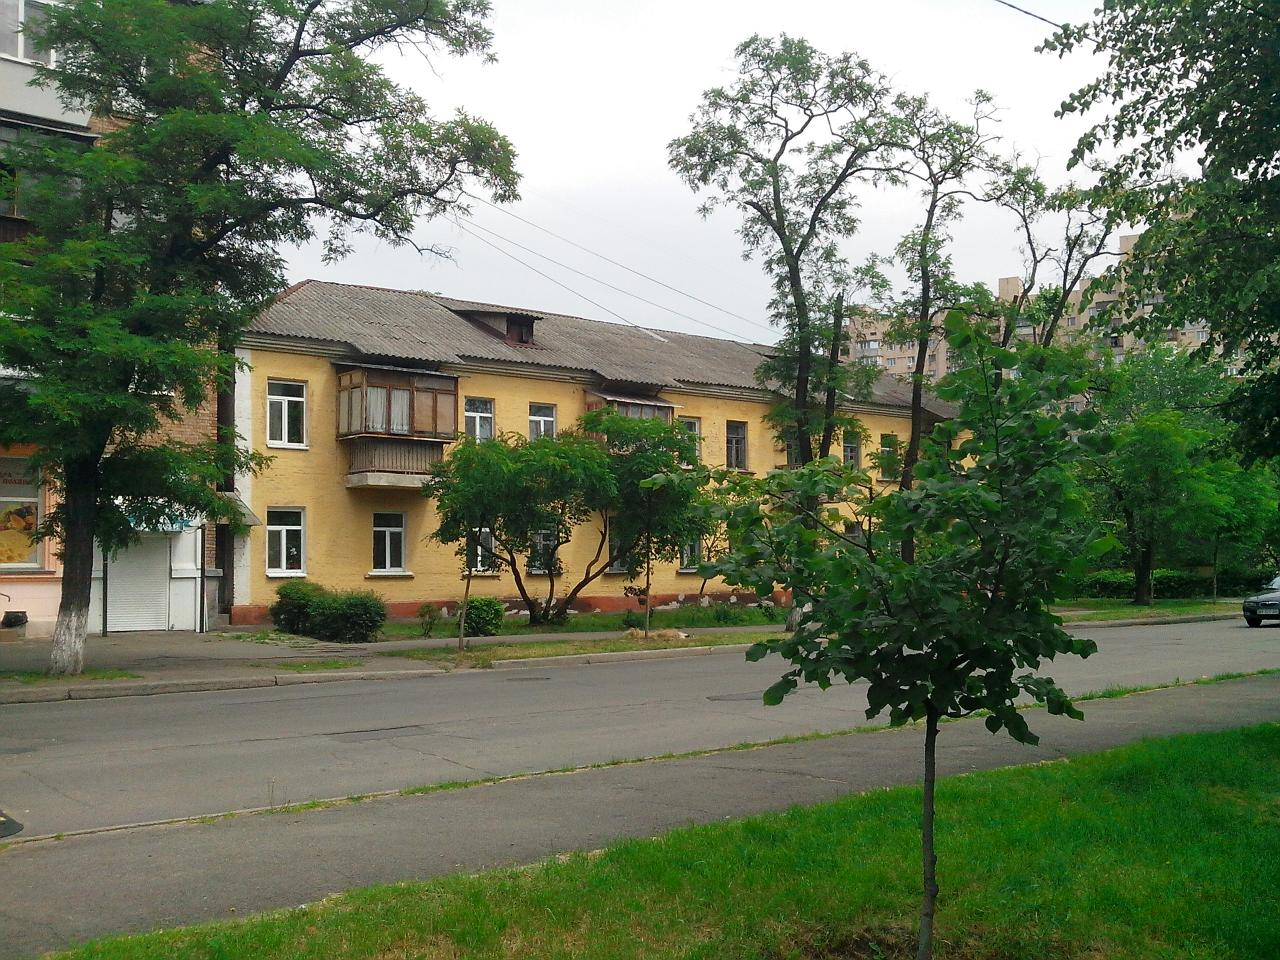
\includegraphics[width=\linewidth]{lpix/IMG_20160613_143139.jpg}

\textit{Новая Дарница.}
\end{center}

\newpage
\begin{center}
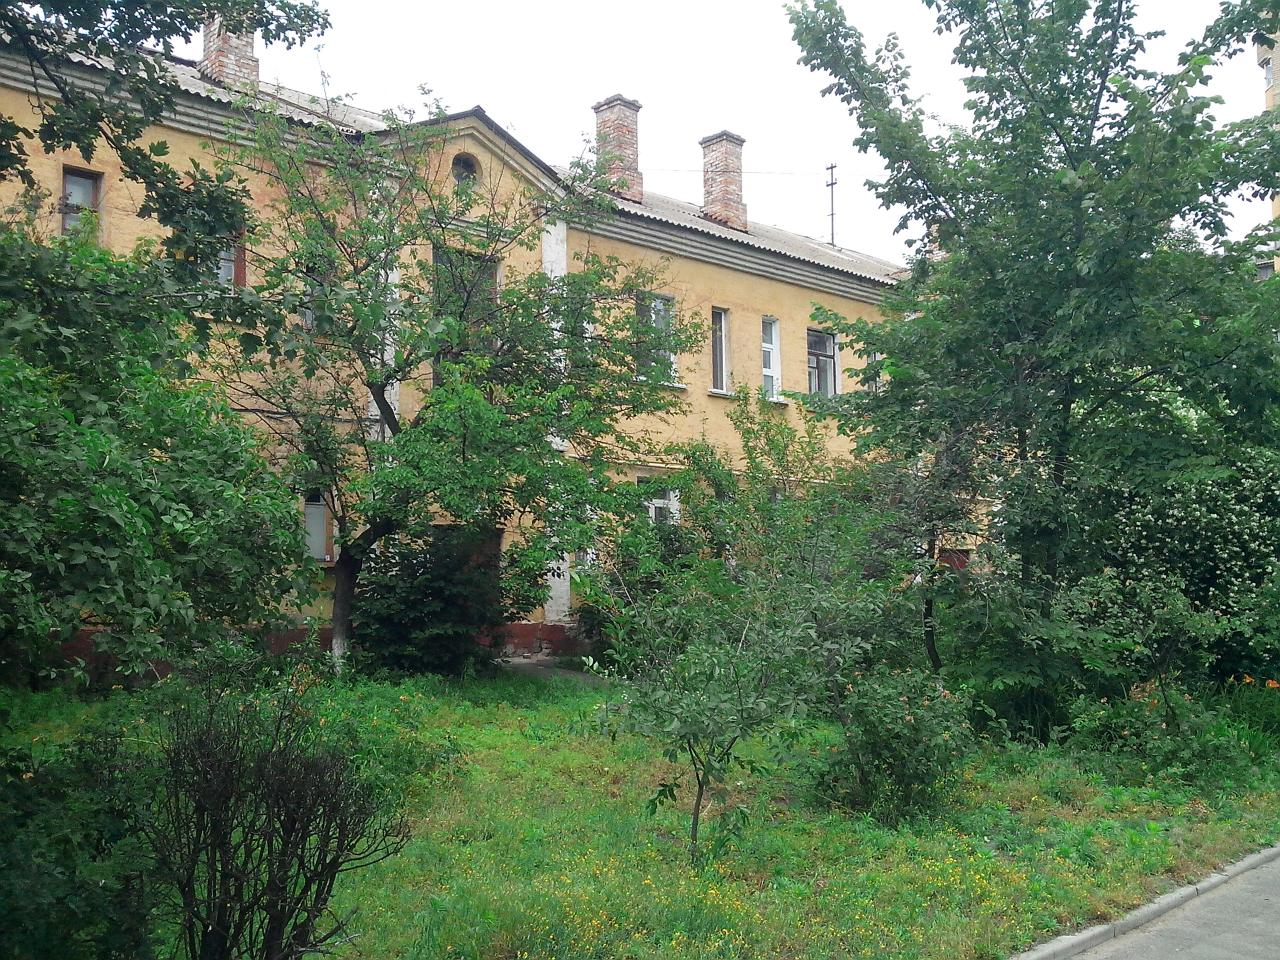
\includegraphics[width=\linewidth]{lpix/IMG_20160613_143545.jpg}

\textit{Новая Дарница.}
\end{center}


\begin{center}
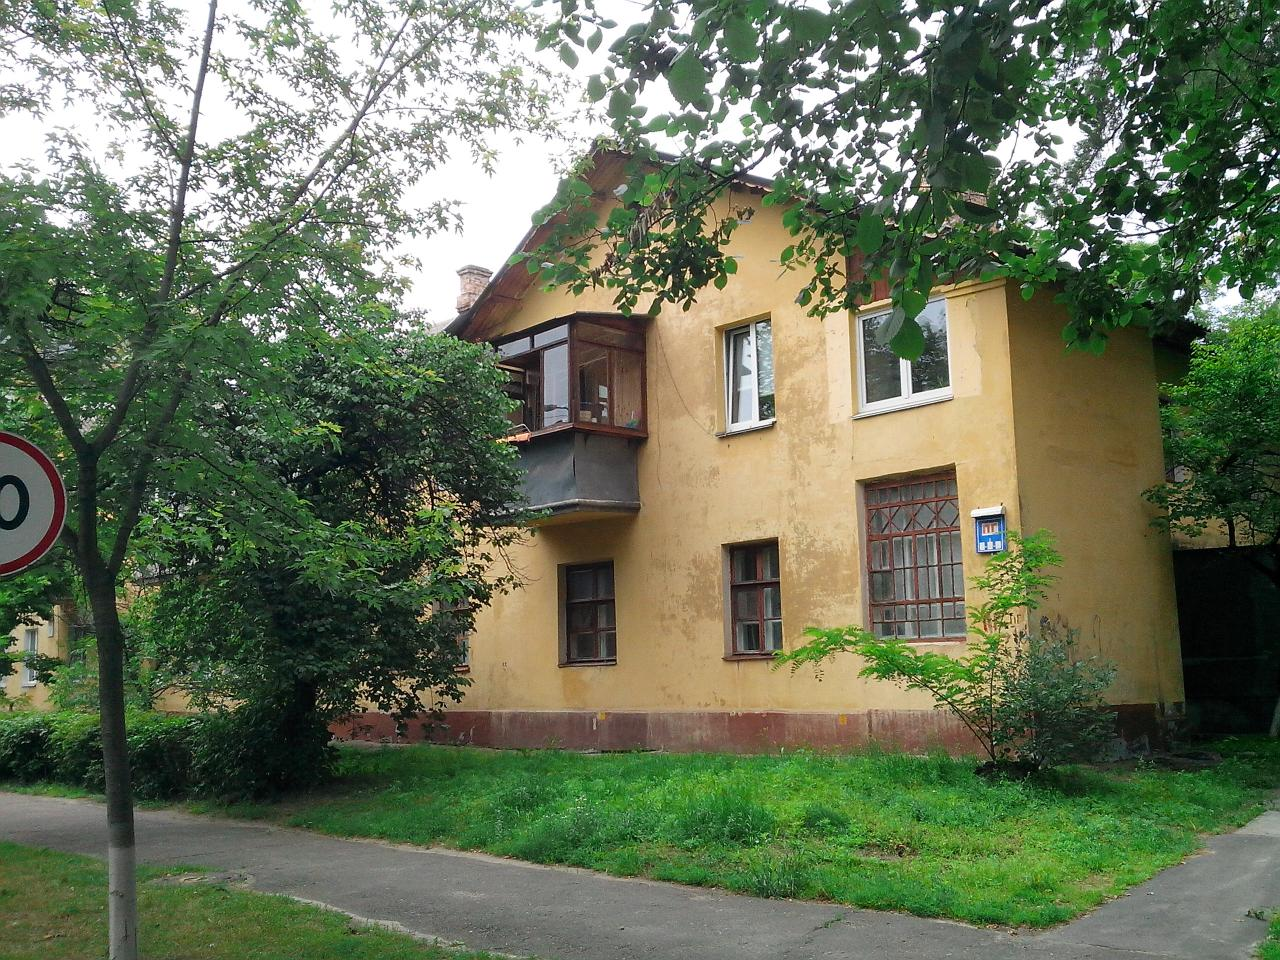
\includegraphics[width=\linewidth]{lpix/IMG_20160613_143641.jpg}

\textit{Новая Дарница.}
\end{center}
\newpage


\begin{center}
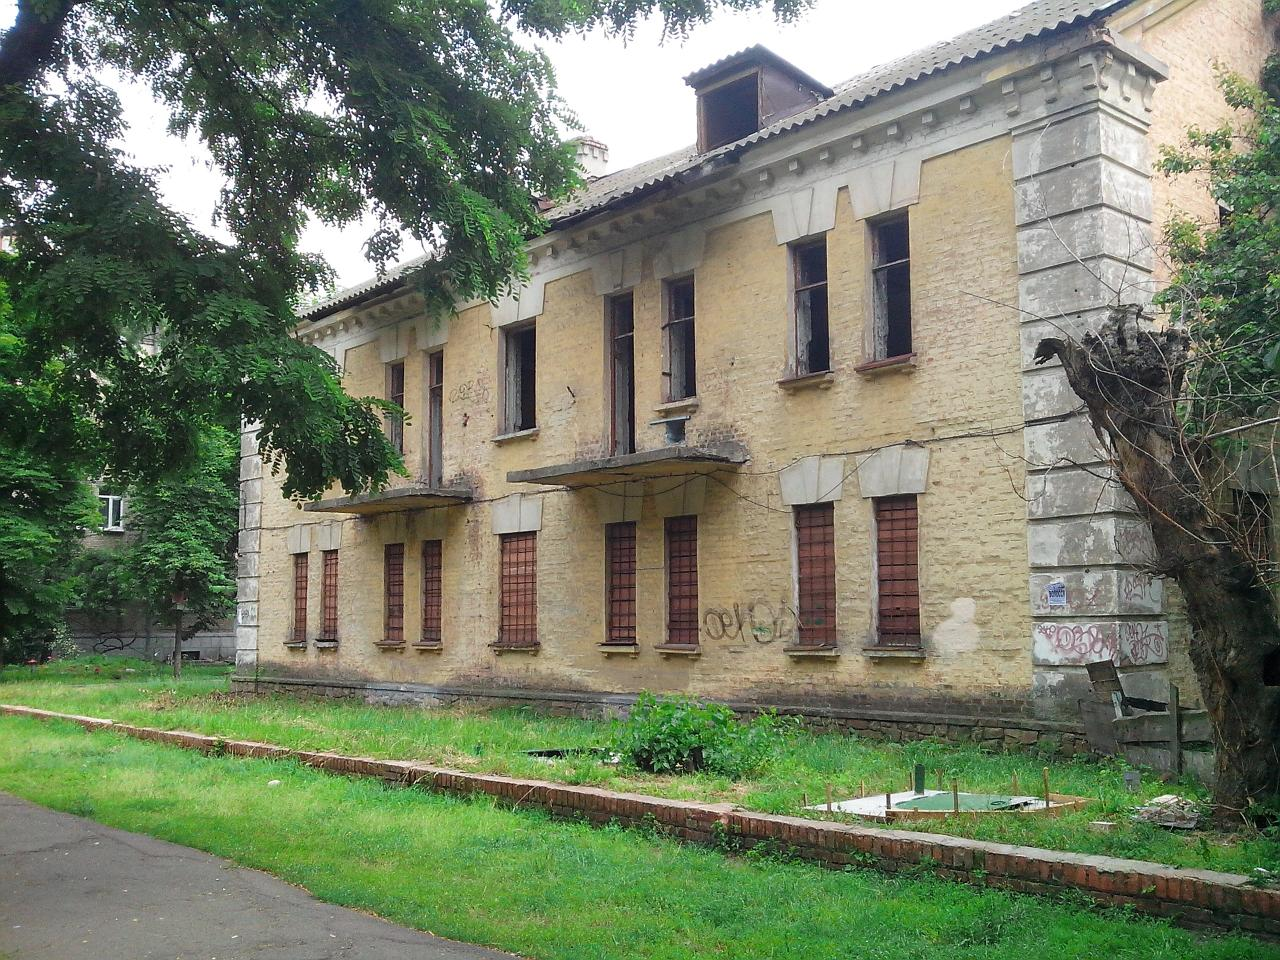
\includegraphics[width=\linewidth]{lpix/IMG_20160613_143848.jpg}

\textit{Новая Дарница.}
\end{center}

\begin{center}
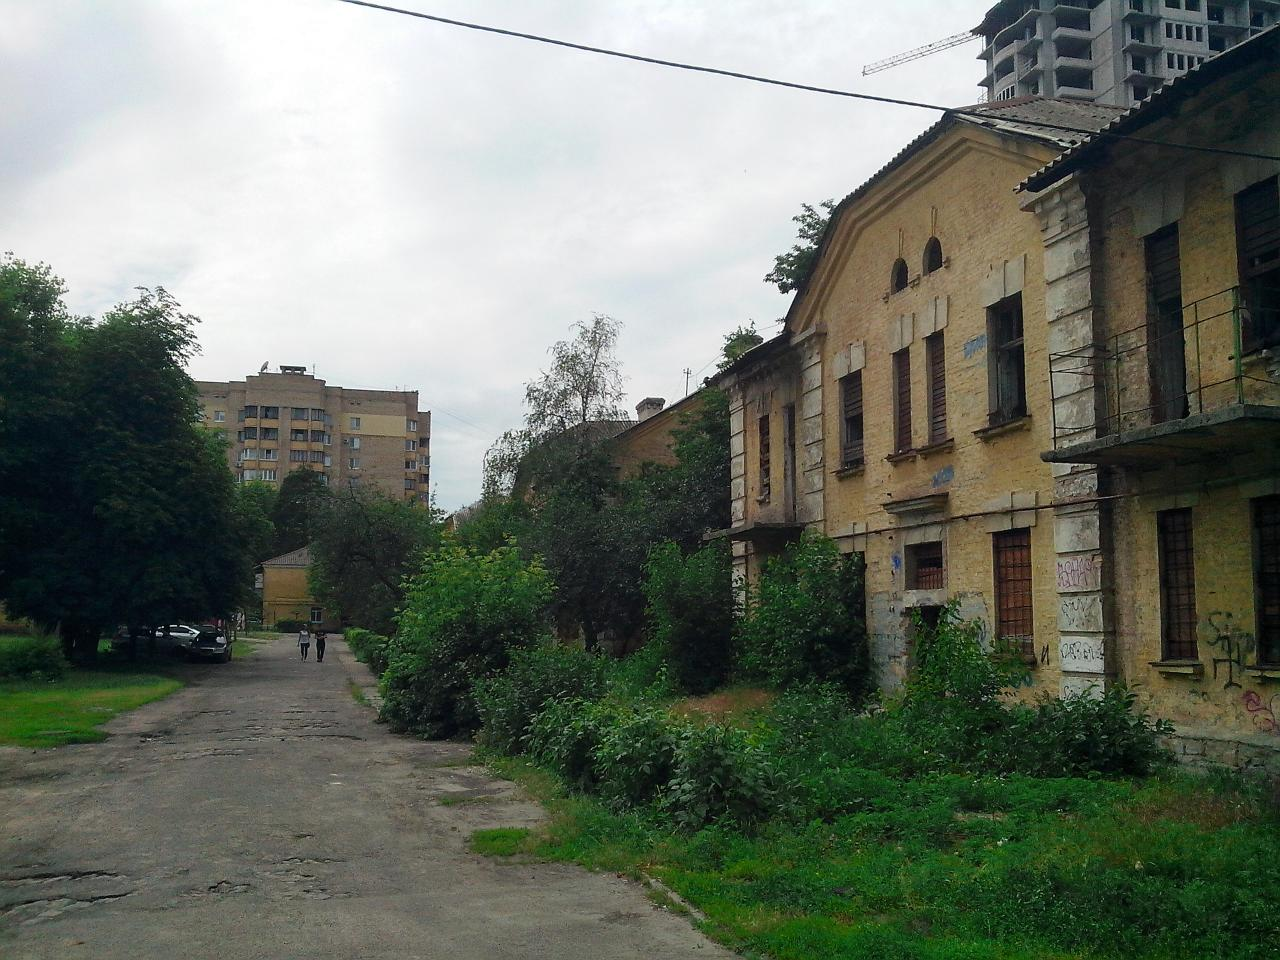
\includegraphics[width=\linewidth]{lpix/IMG_20160613_143926.jpg}

\textit{Новая Дарница.}
\end{center}
\newpage

\begin{center}
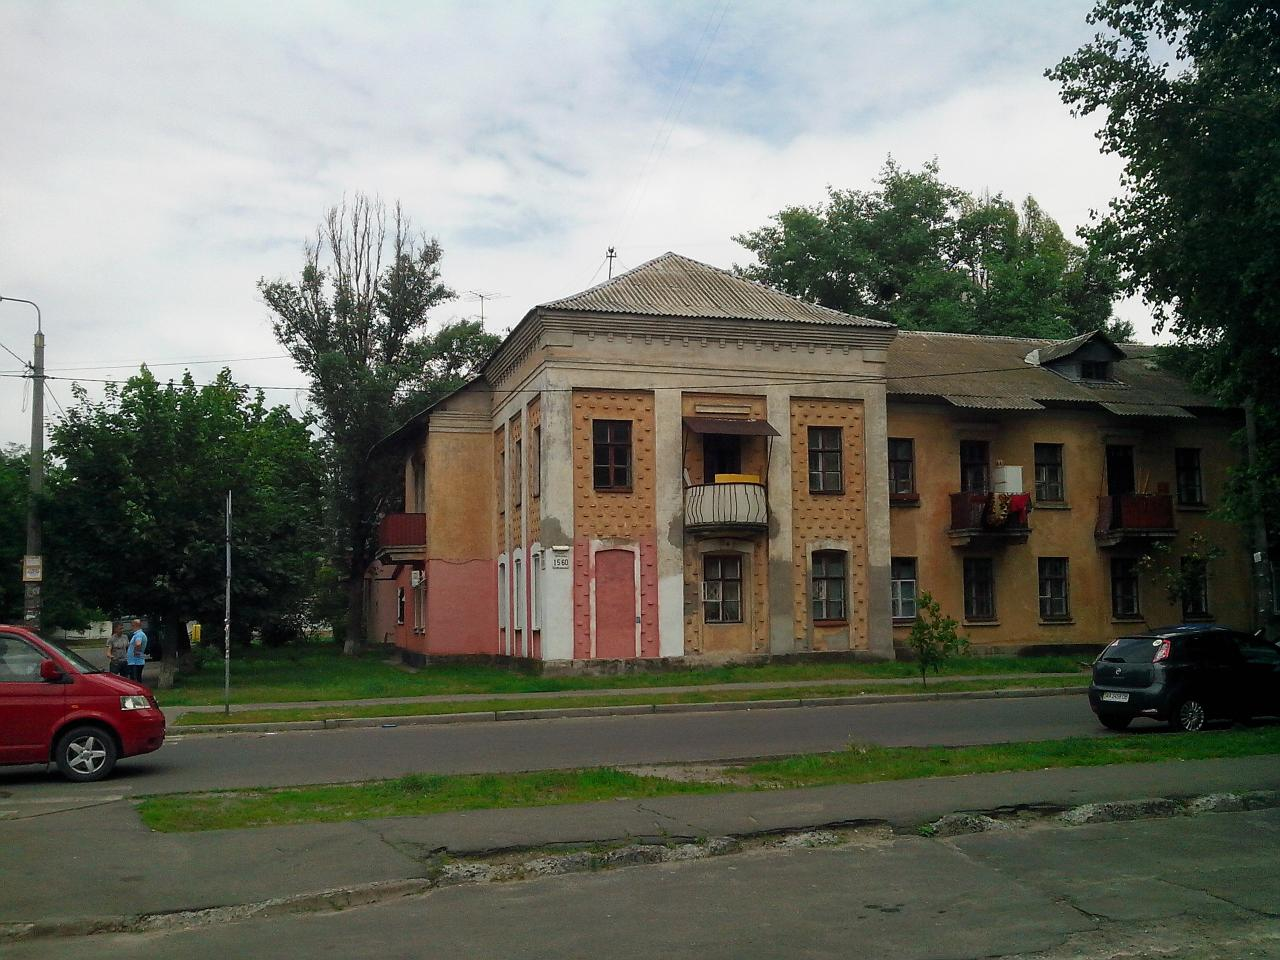
\includegraphics[width=\linewidth]{lpix/IMG_20160613_145115.jpg}

\textit{Новая Дарница. Волгодонская улица.}
\end{center}

\begin{center}
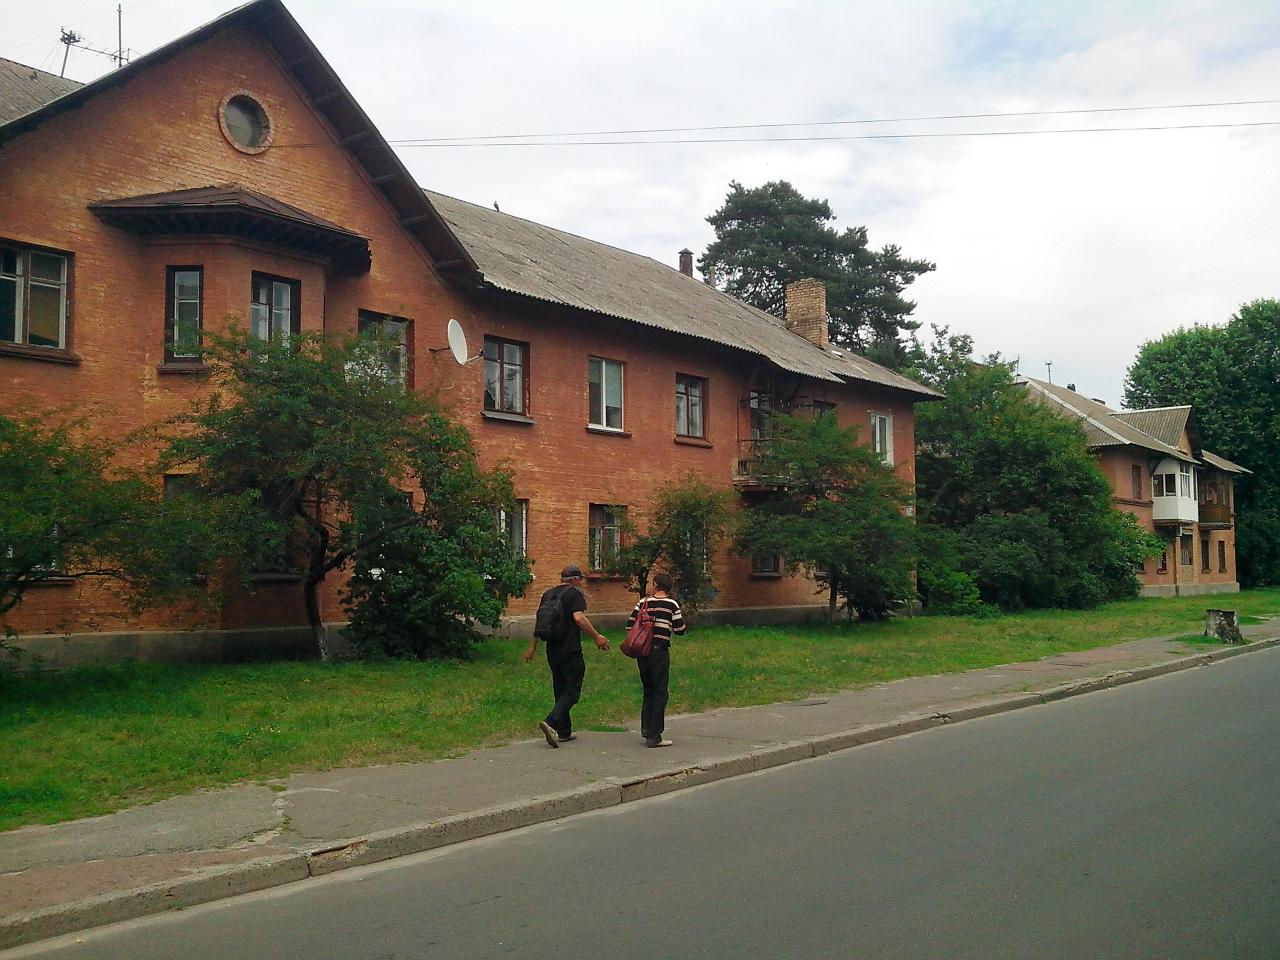
\includegraphics[width=\linewidth]{lpix/IMG_20160613_145313.jpg}

\textit{Новая Дарница. Волгодонская улица.}
\end{center}
\newpage


\begin{center}
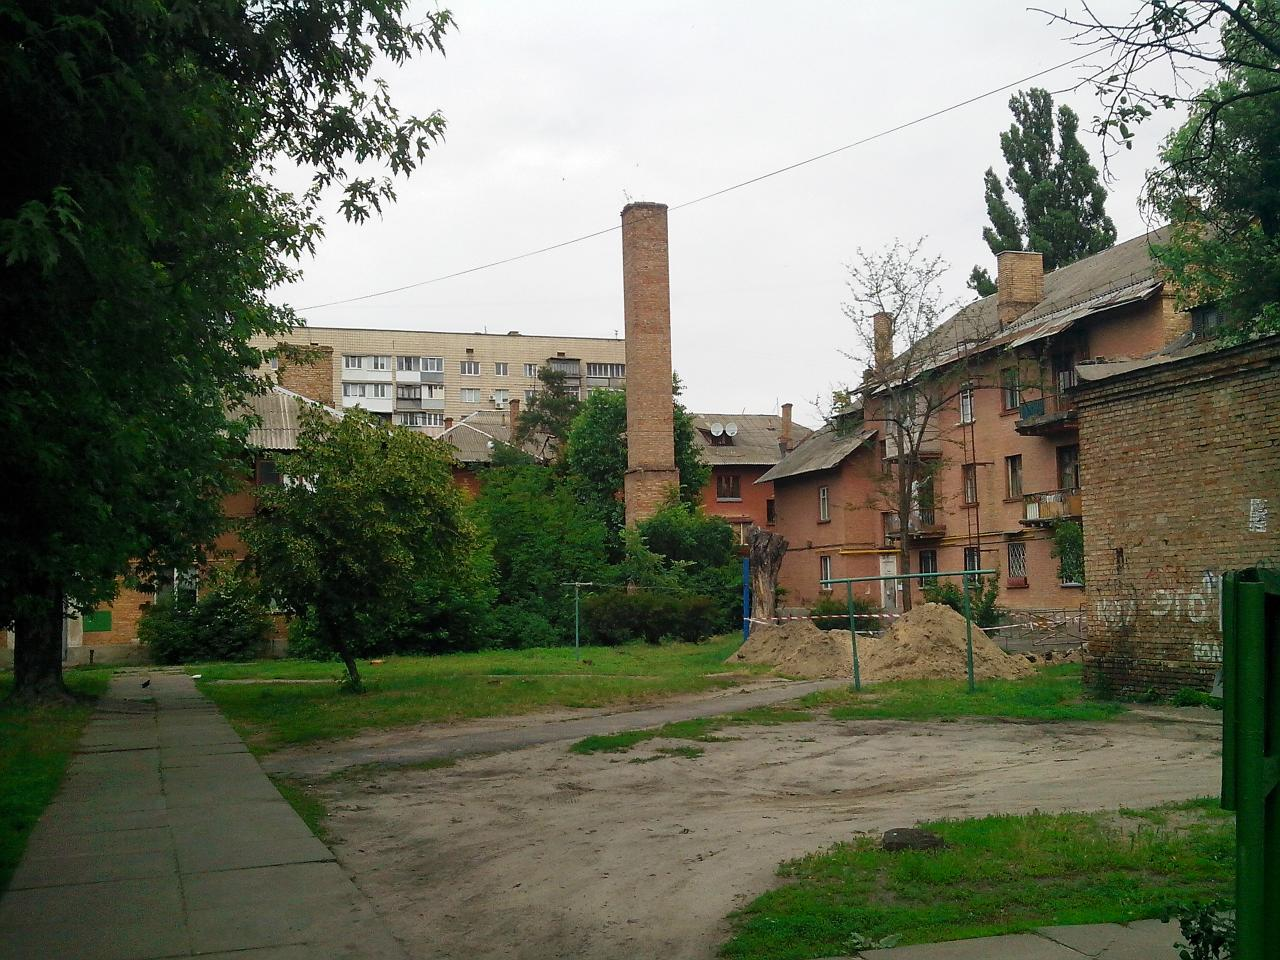
\includegraphics[width=\linewidth]{lpix/IMG_20160613_145450.jpg}

\textit{Новая Дарница. Волгодонская улица.}
\end{center}


\begin{center}
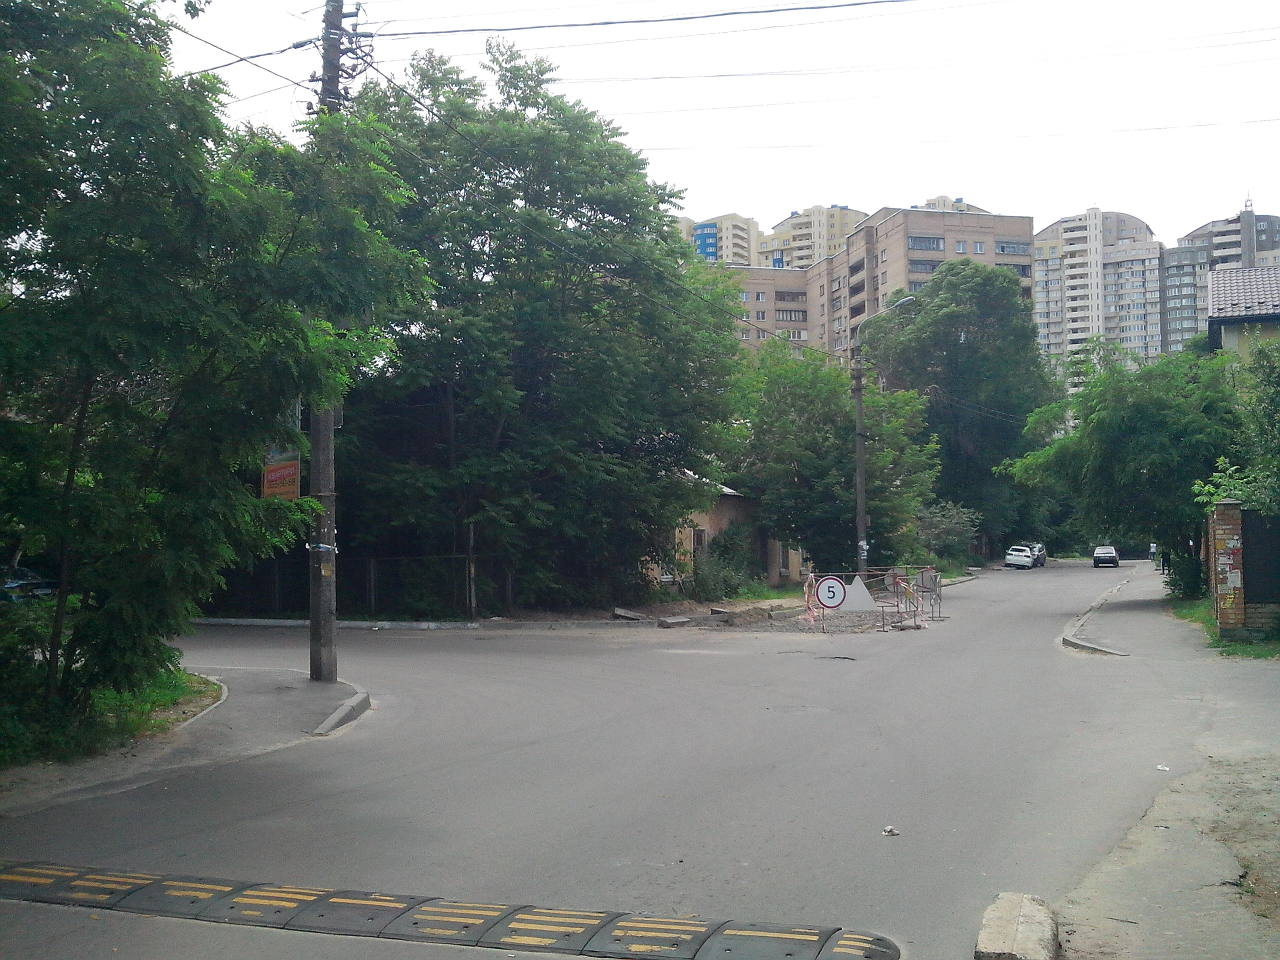
\includegraphics[width=\linewidth]{lpix/IMG_20160613_140013.jpg}

\textit{Старая Дарница. Двинская улица.}
\end{center}

\begin{center}
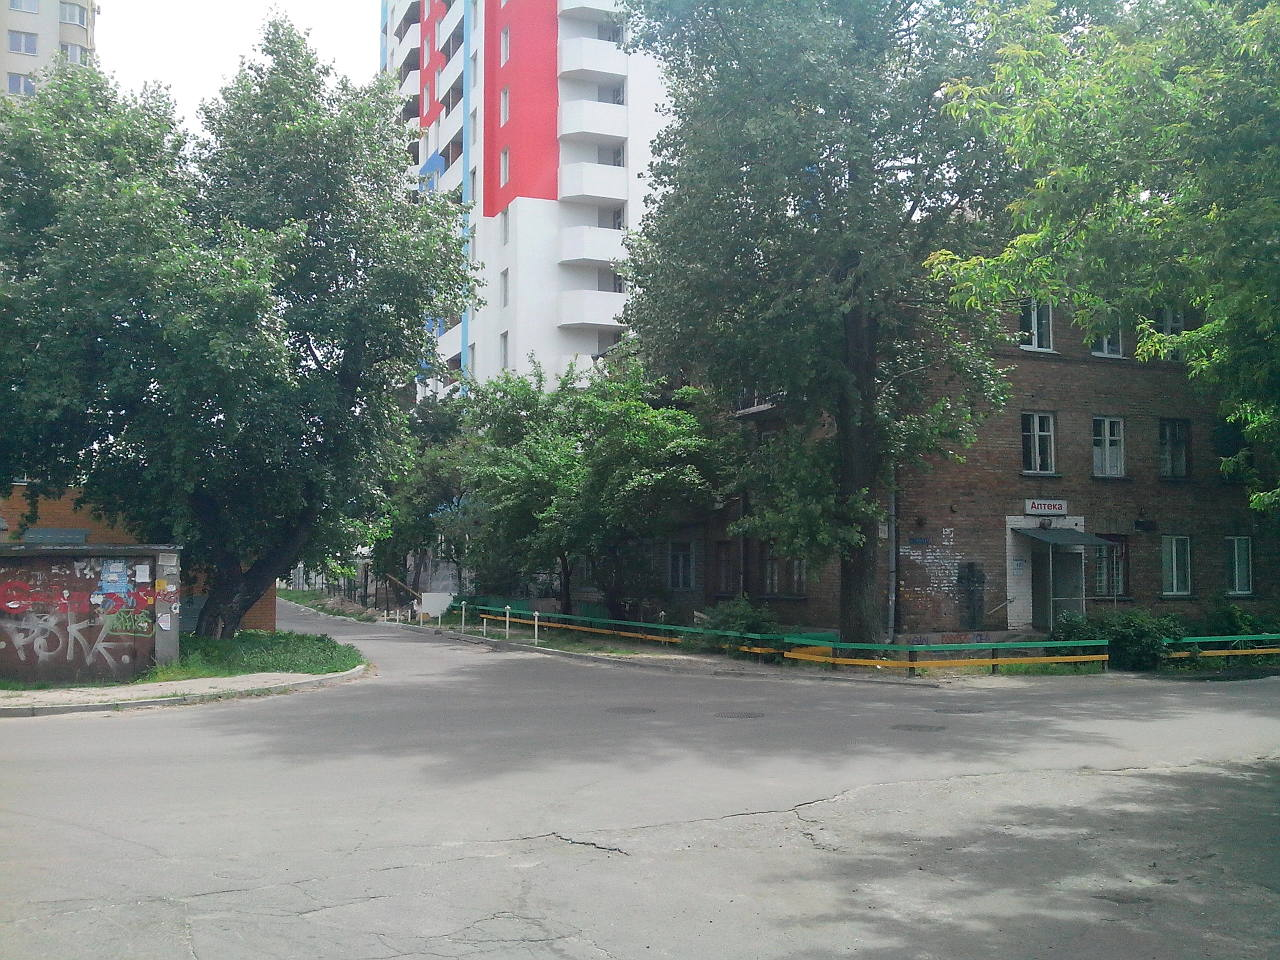
\includegraphics[width=\linewidth]{lpix/IMG_20160613_140125.jpg}

\textit{Старая Дарница. Двинская улица.}
\end{center}


\begin{center}
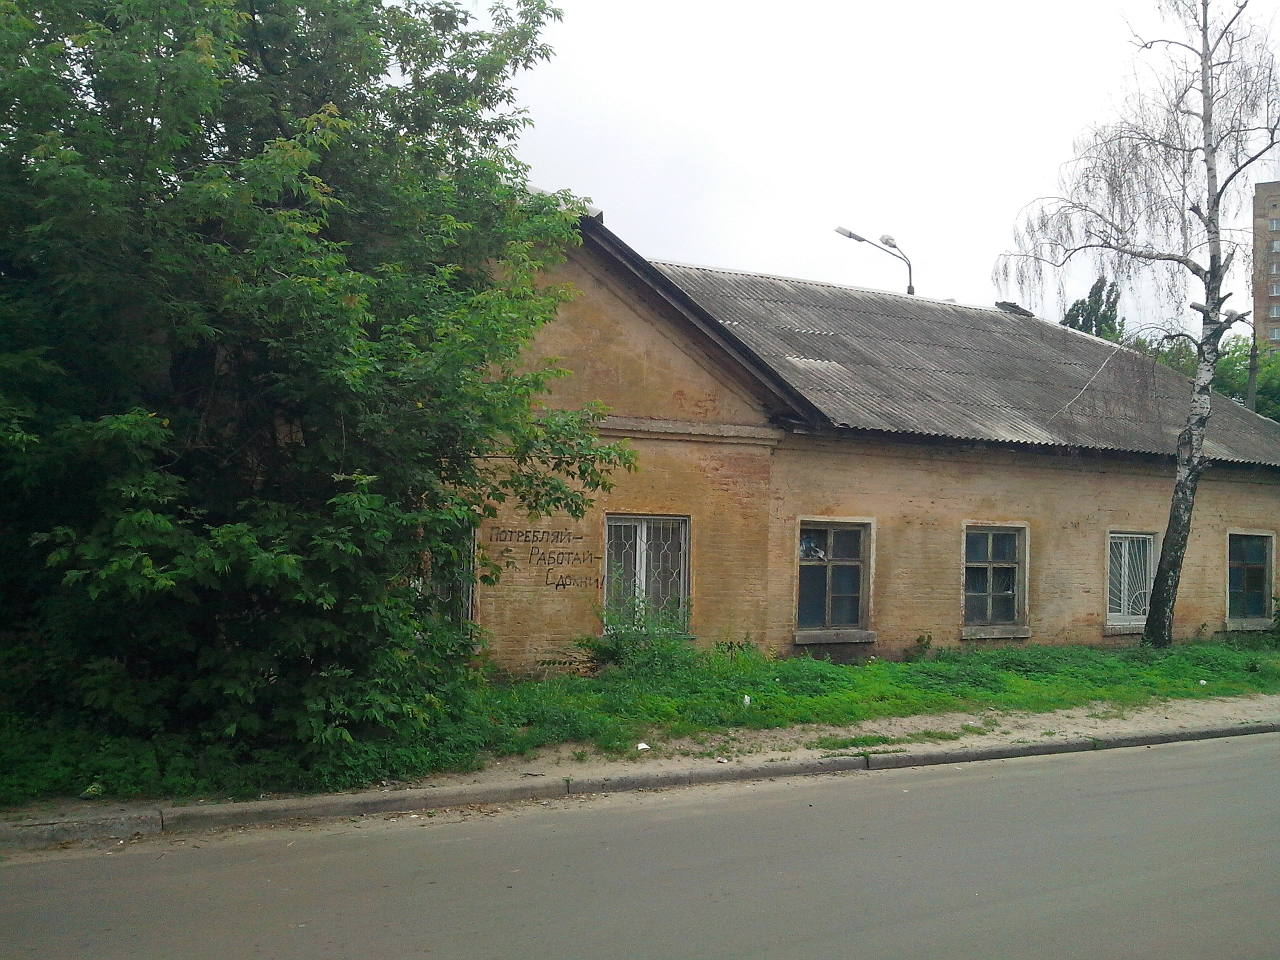
\includegraphics[width=\linewidth]{lpix/IMG_20160613_140440.jpg}

\textit{Старая Дарница. Двинская улица.}
\end{center}


\begin{center}
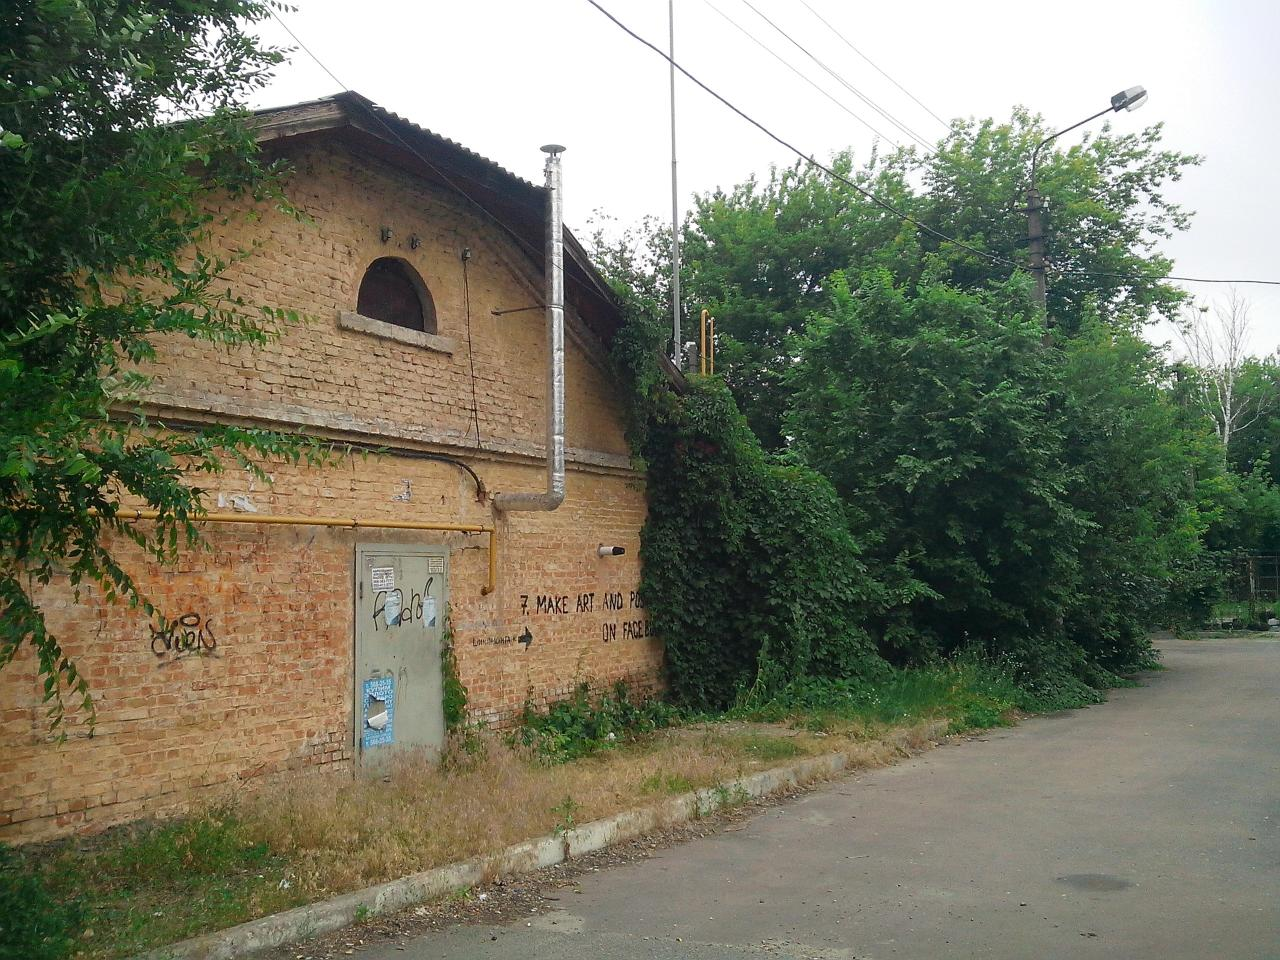
\includegraphics[width=\linewidth]{lpix/IMG_20160613_140656.jpg}

\textit{Старая Дарница. Двинская улица.}
\end{center}


\begin{center}
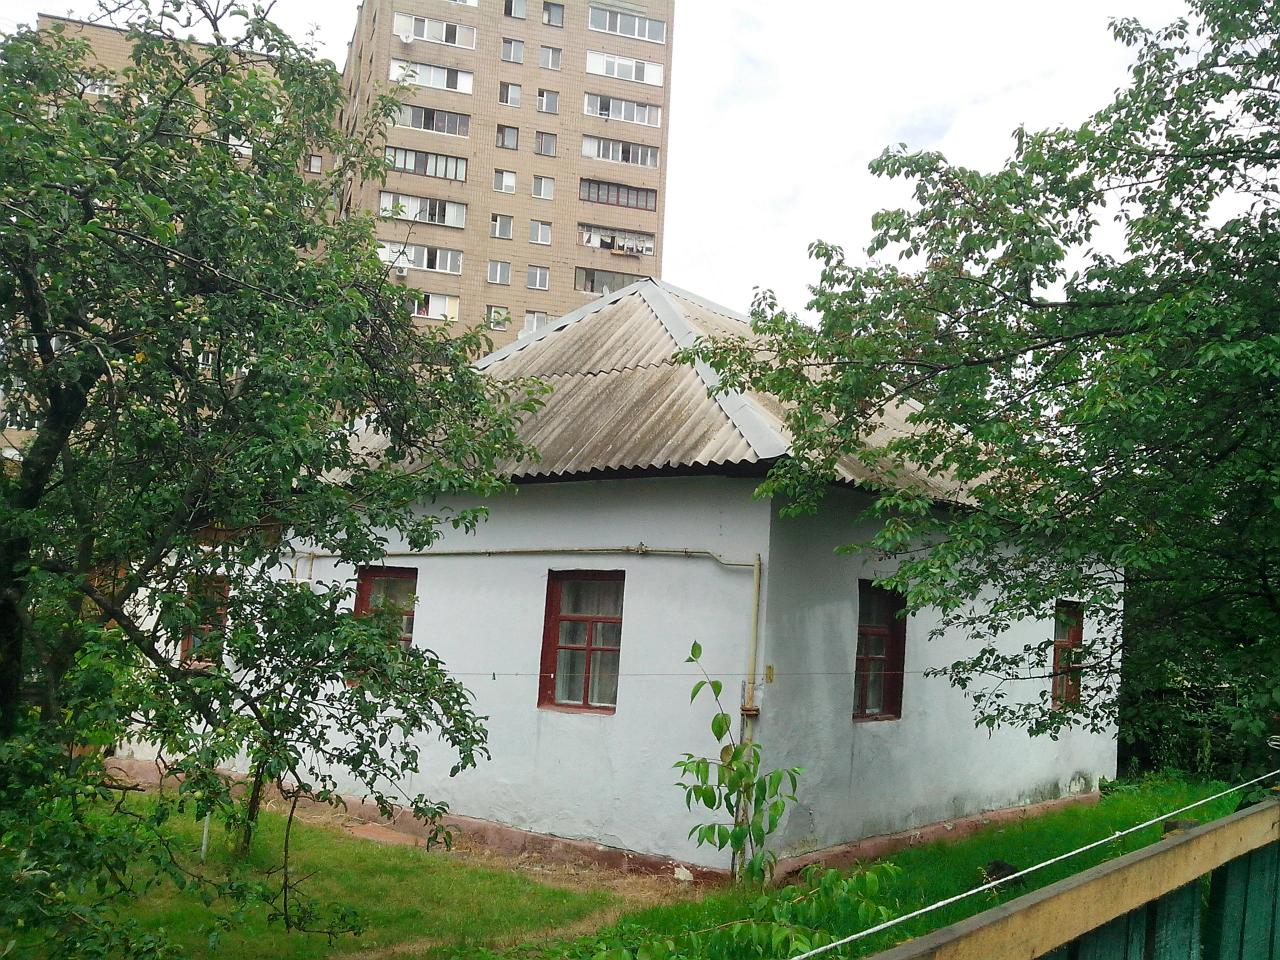
\includegraphics[width=0.95\linewidth]{lpix/IMG_20160613_141059.jpg}

\textit{Старая Дарница. Окрестности Сновской улицы.}
\end{center}


\begin{center}
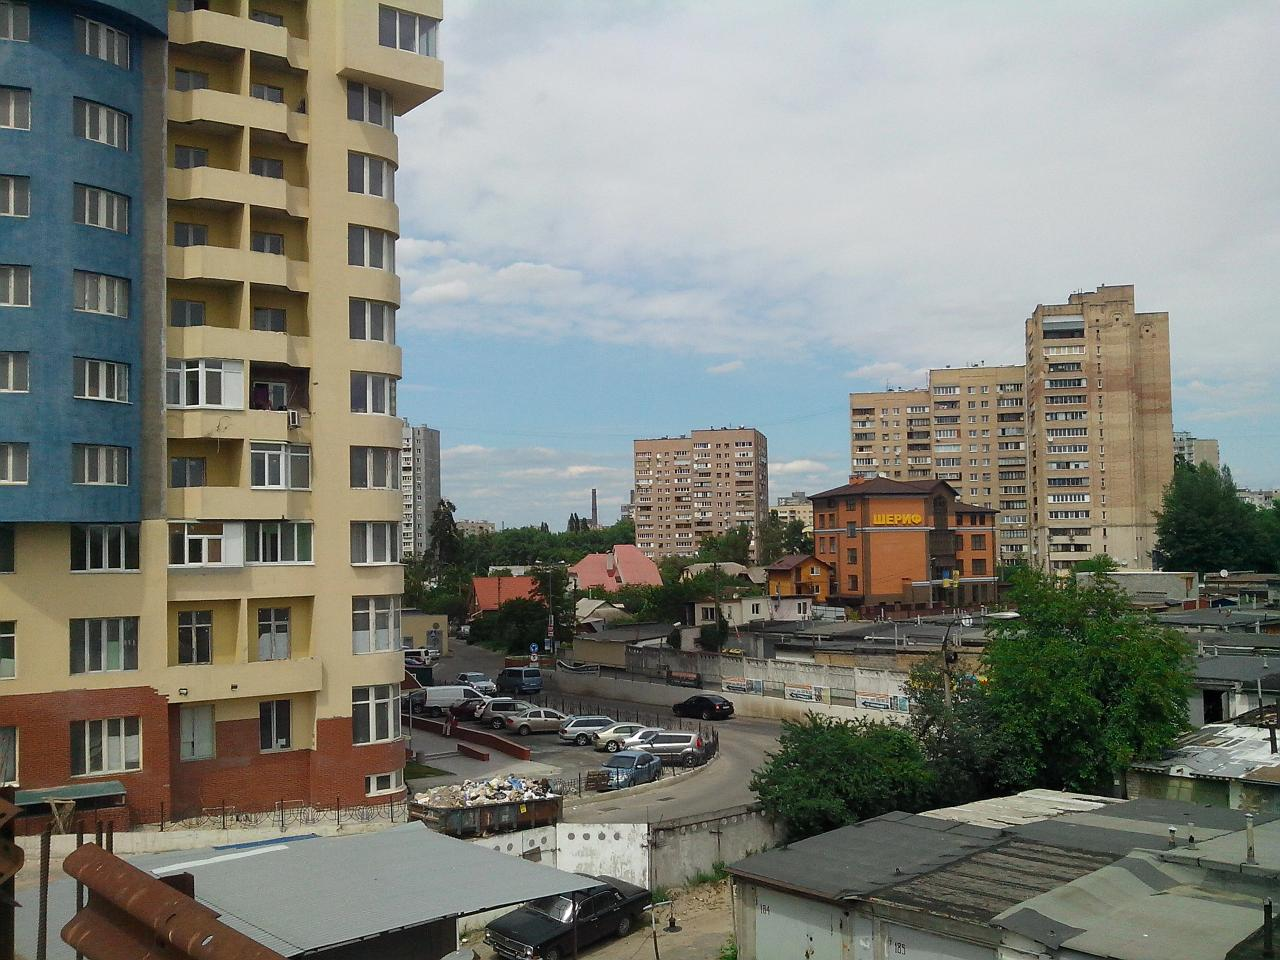
\includegraphics[width=0.95\linewidth]{lpix/IMG_20160613_141738.jpg}

\textit{Старая Дарница. Окрестности Сновской.}
\end{center}


\begin{center}
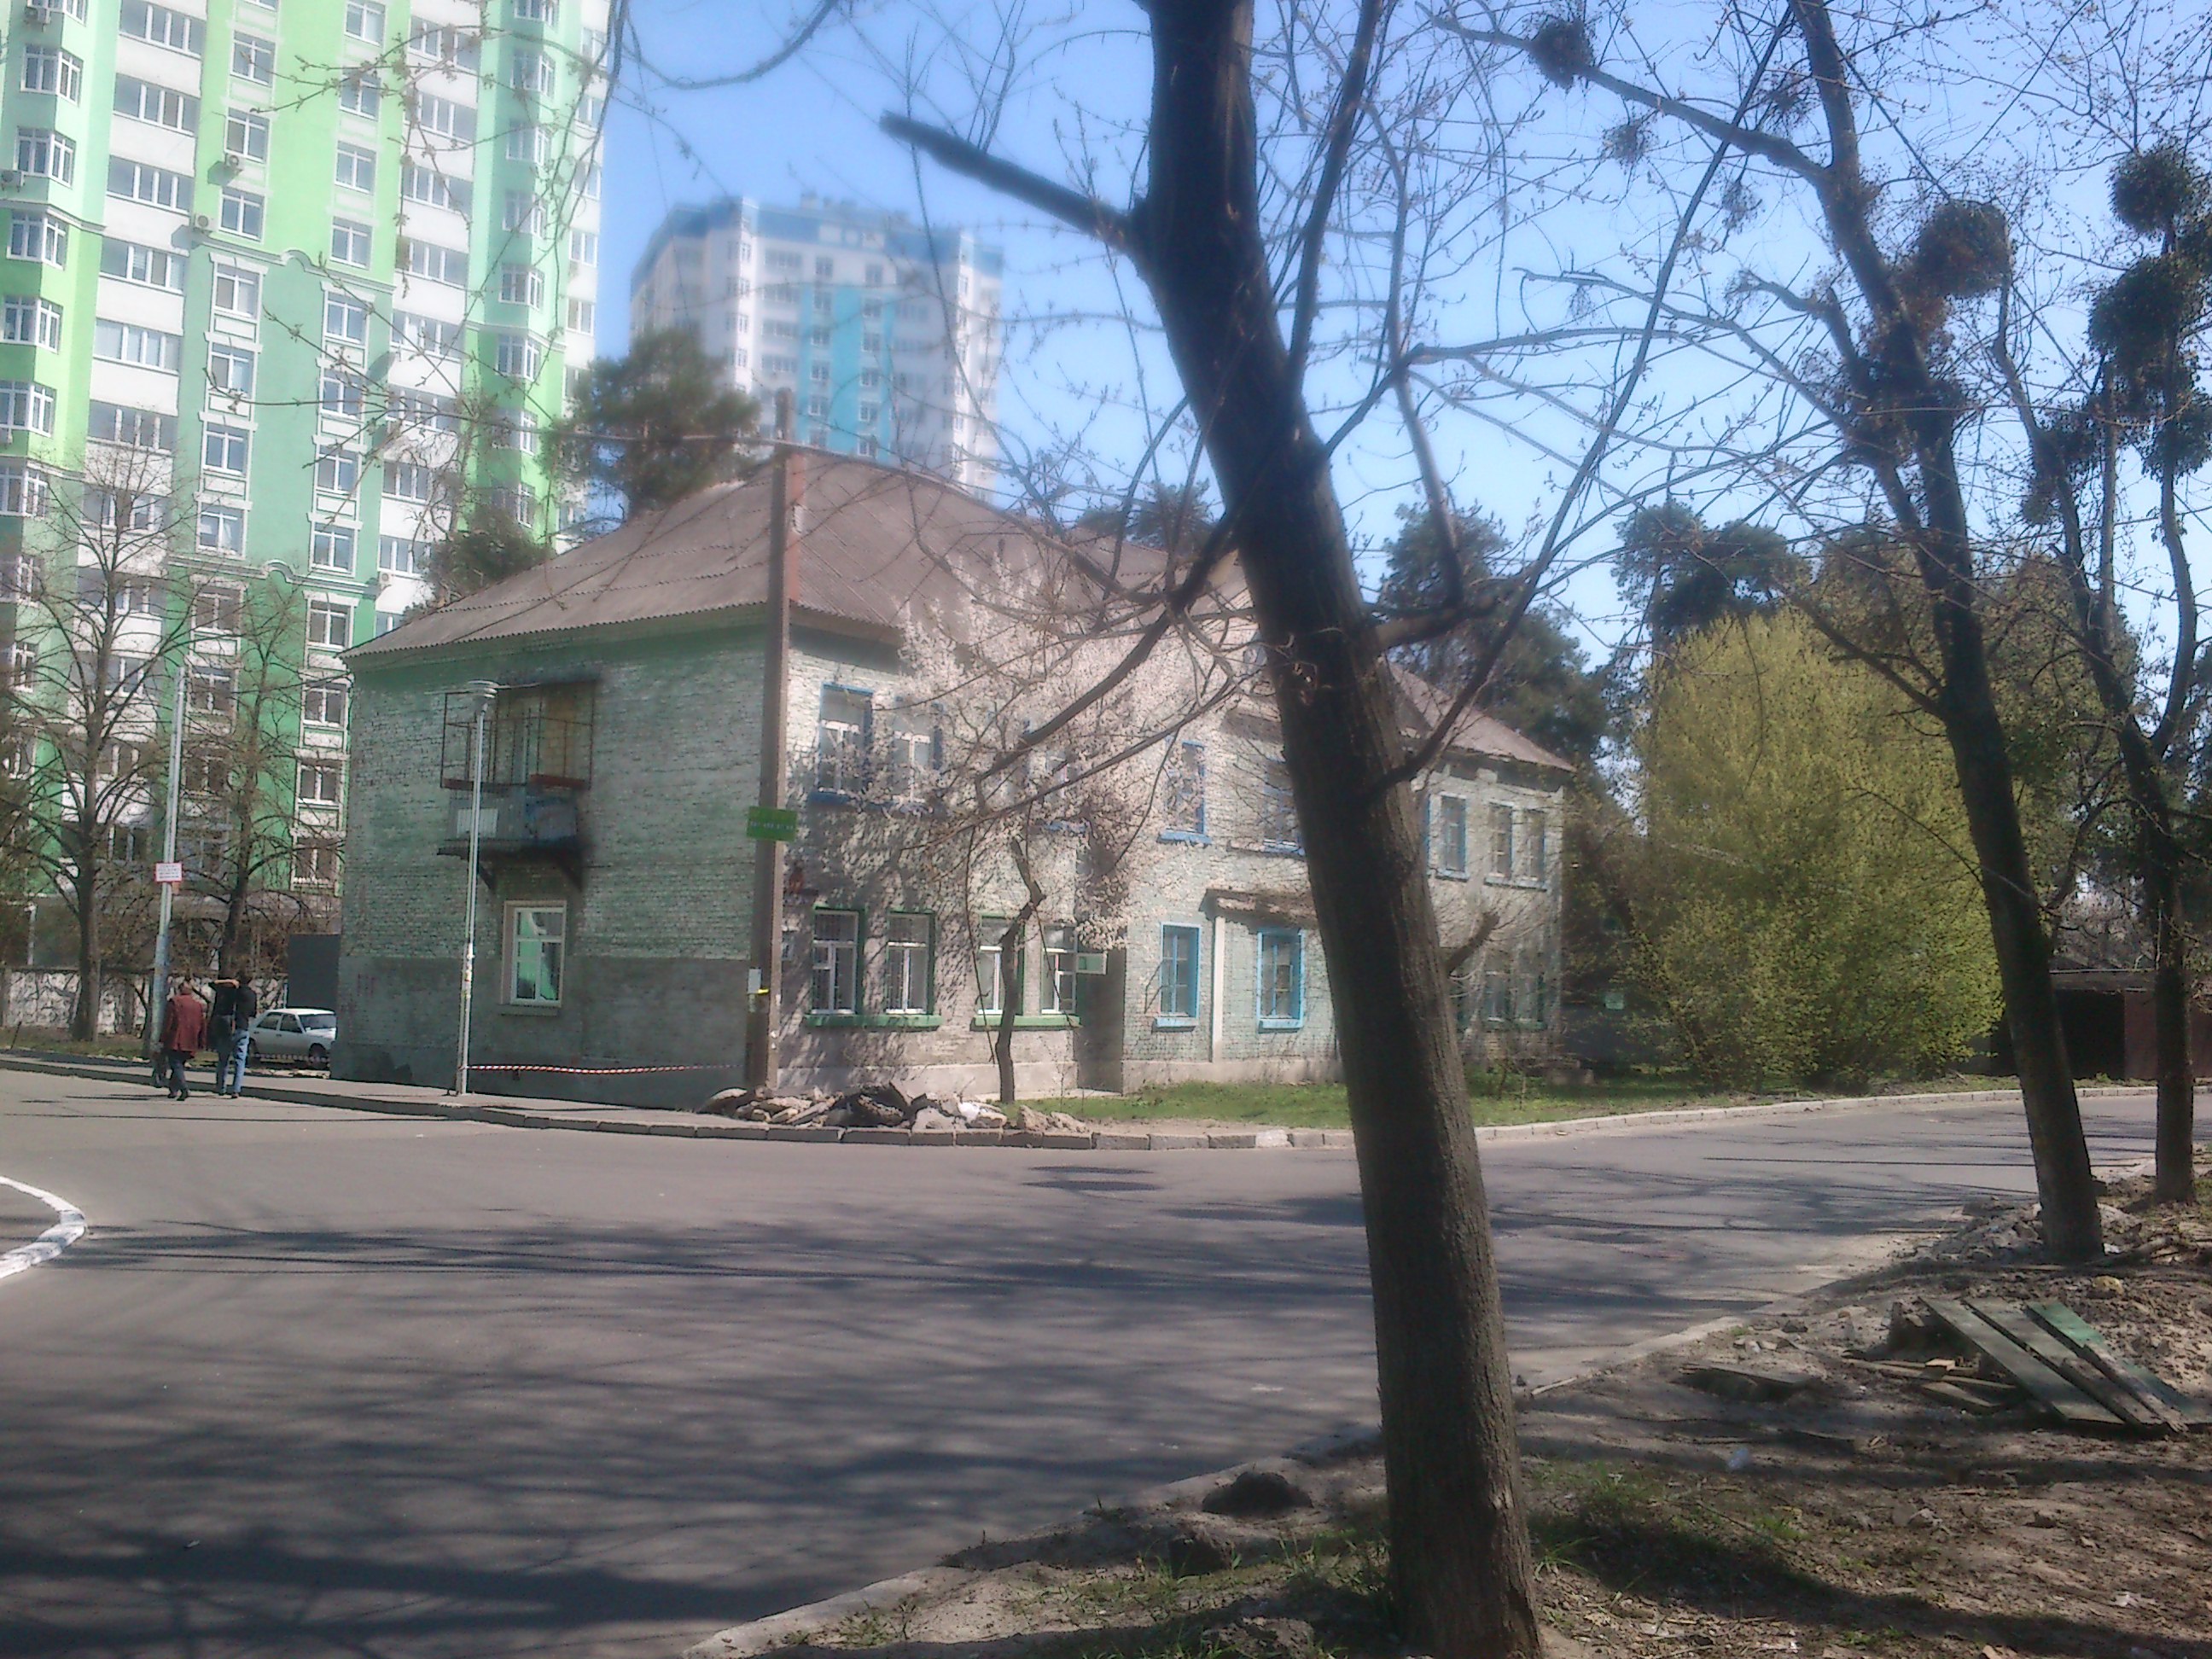
\includegraphics[width=\linewidth]{lpix/DSC_0013.JPG}

\textit{Поселок Ремзавода.}
\end{center}


\begin{center}
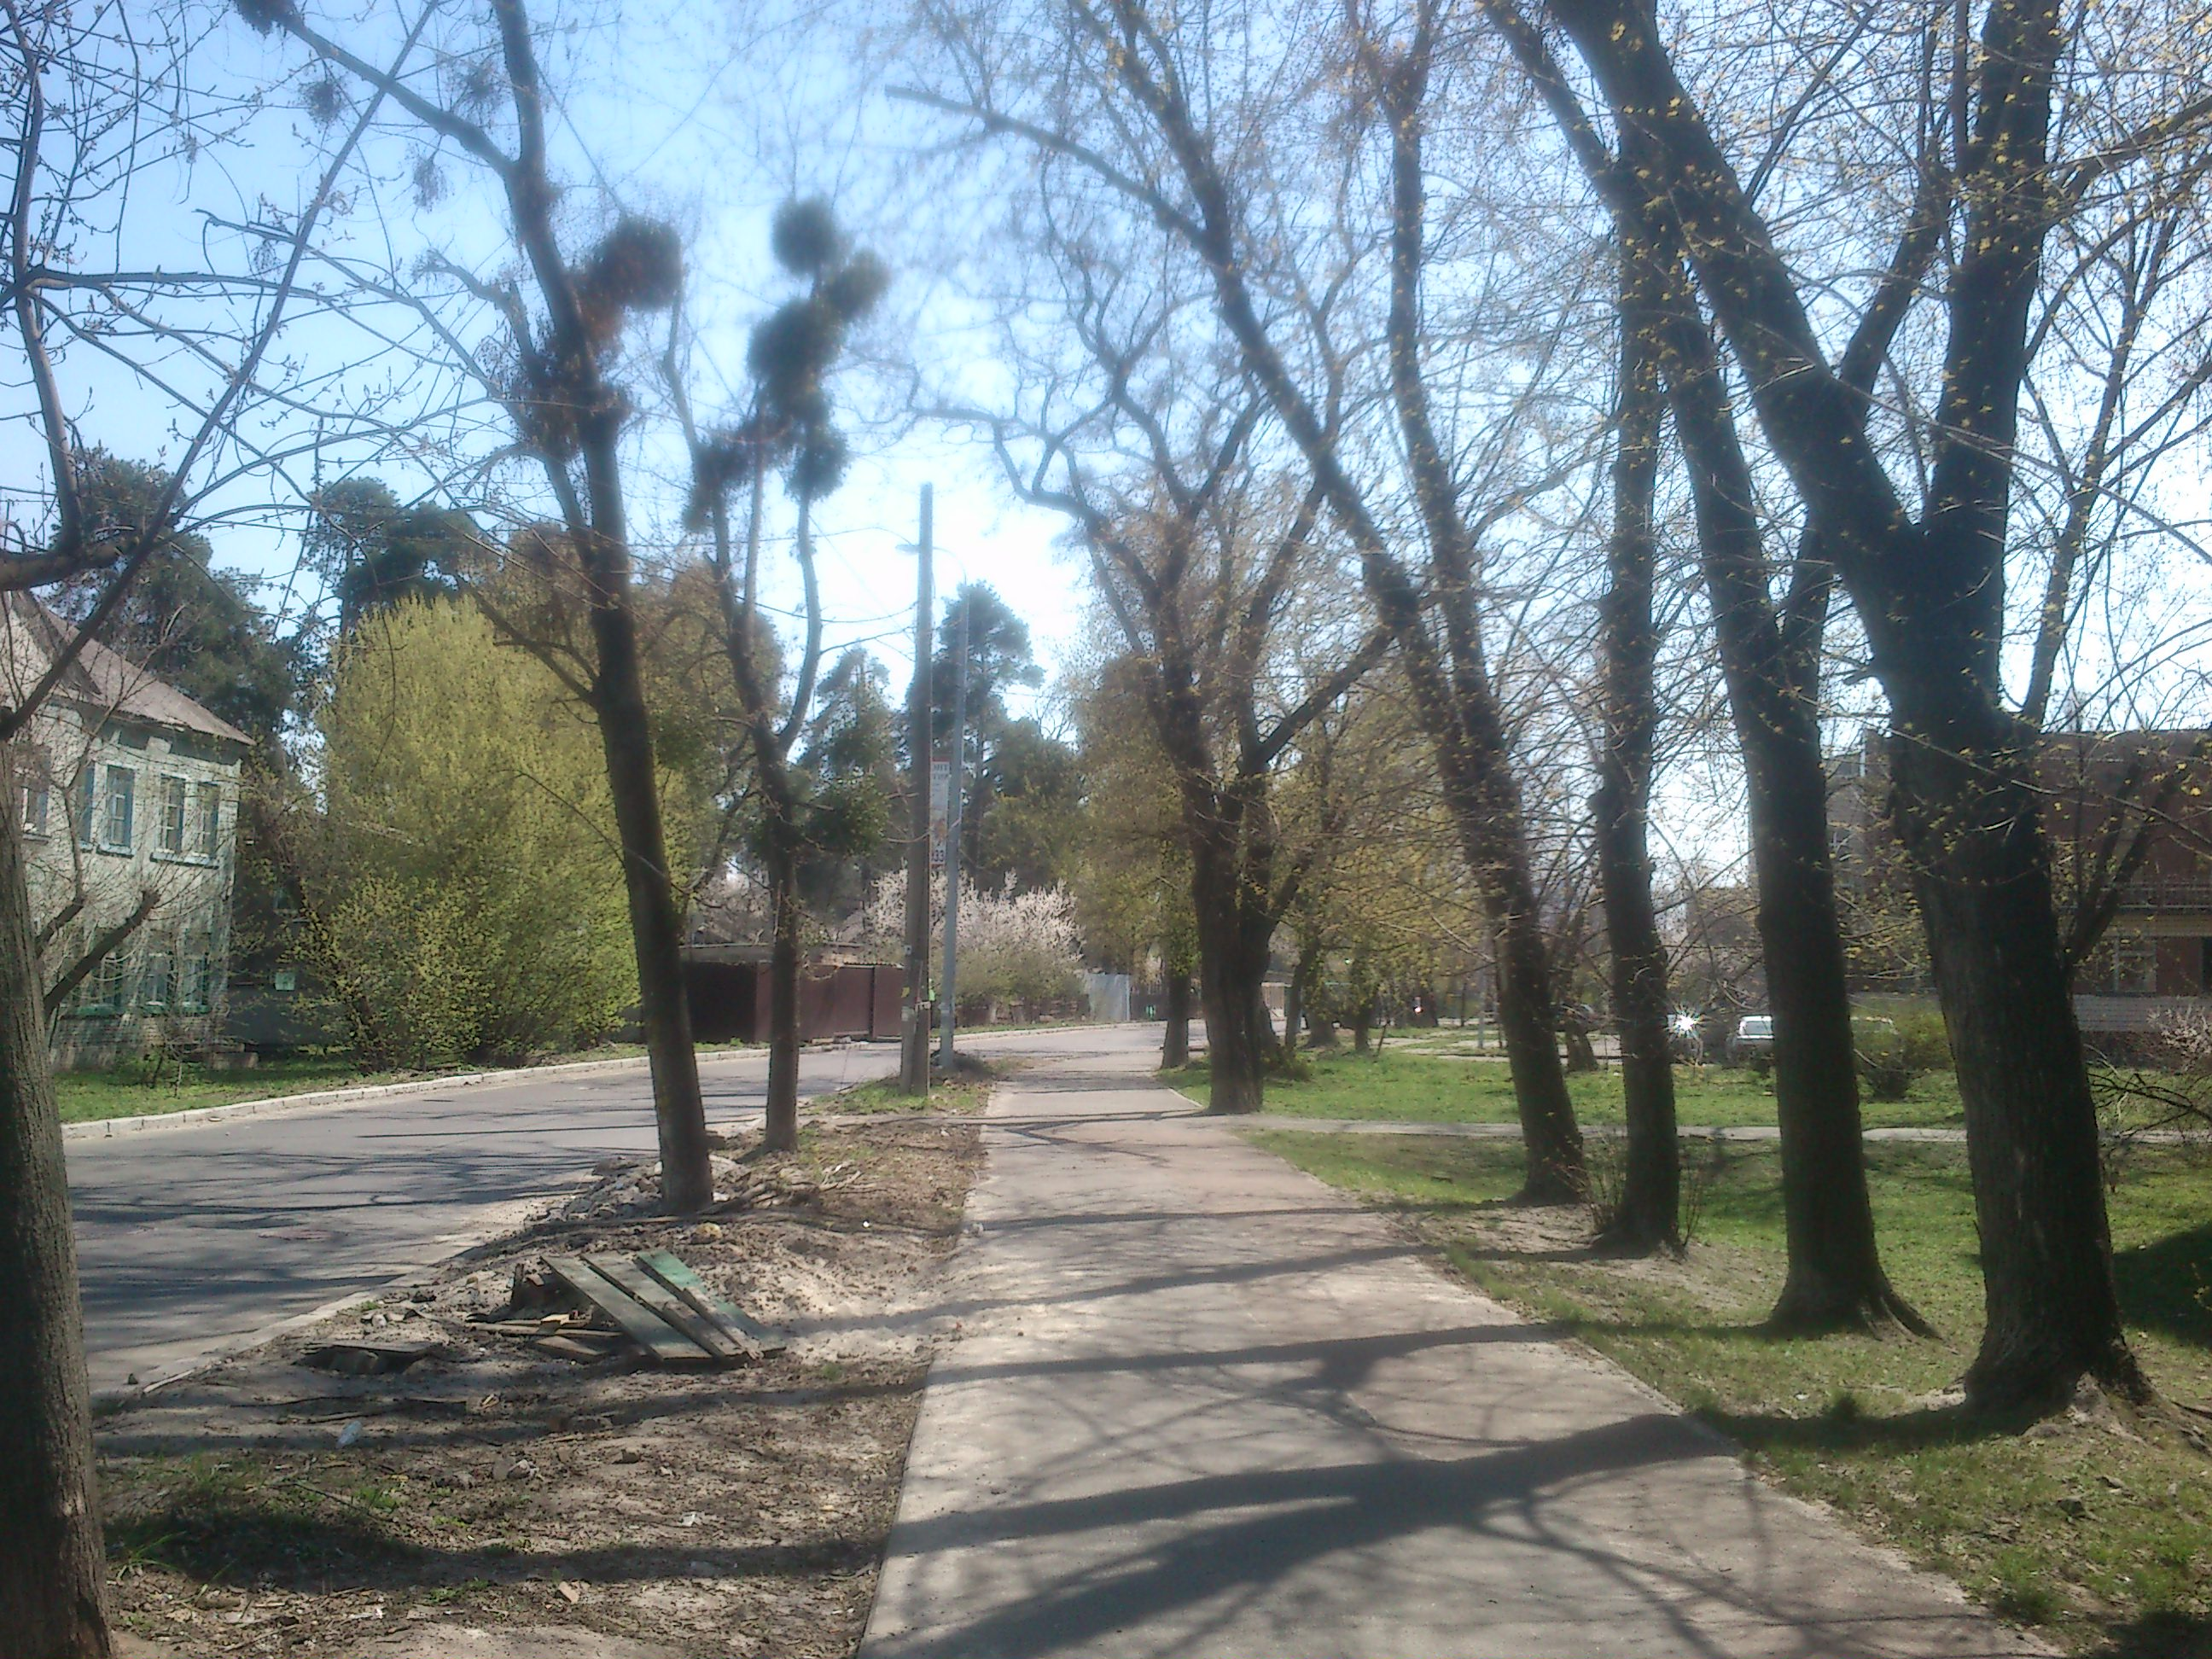
\includegraphics[width=\linewidth]{lpix/DSC_0014.JPG}

\textit{Поселок Ремзавода.}
\end{center}


\begin{center}
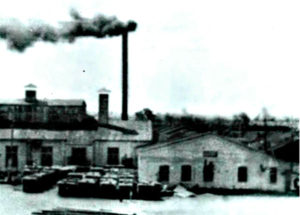
\includegraphics[width=0.95\linewidth]{lpix/gabel.jpg}

\textit{Фанерный завод братьев Габель.}
\end{center}



\part{Правый берег}

\chapter*{А}
\addcontentsline{toc}{chapter}{А}


\textbf{Авиагородок} – район, лежащий на северо-запад от станции метро «Святошин». Ограничен проспектом Победы, бульваром Вернадского, улицей Краснова и железной дорогой. Изначально был застроен частными домами работников близлежащего (к востоку) авиазавода (ныне «Антонов»). Сейчас там дома всех сортов – остаток частного сектора, двухэтажки, хрущовки.\\

\medskip

\textbf{Автострада} – старое название бульвара Дру\-жбы Народов. Дорога эта прежде, еще в начале 20 века, не существовала, ее место занимали овраги да бугры, а их старательно обходила грунтовка, проходящая сначала на отрезке нынешнего бульвара около ултцы Филатова, а затем сворачивающая на улицу Ивана Кудри, и примерно совпадающая с последней до ее соединения с бульваром Леси Украинки, где на то время уже была широкая дорога. Грунтовка на 1930 год стала Боинским переулком, от появившейся в ее низовье бойни, занявшей место от современного котлована озера Глинки и пространство Лыбедской площади, и низовье этой дороги сместилось на северо-запад. Так вся дорога стала полностью совпадать с будущей Ивана Кудри.

На немецкой карте 1942 года видим уже расчерченный пунктиром в современных пределах бульвар Дружбы Народов – он именовался Автострадой до 1959 года, и поначалу в самом деле был бульваром, с полосой посередине, где росли деревья.

Но что карта 1942 года, если на немецких аэрофотоснимках лета 1941 года видна проложенная или прокладываемая дорога Автострады, значит ее стали прокладывать еще до оккупации города немцами.

Бульвар застраивался неравномерно, б\'ольшая часть домов советского периода на нем построена со второй половины 1950х и в шестидесятые годы, самый старый – Дружбы Народов, 7 – 1947 года.

По пути Автострады на протяженности от Чешской до Печерского моста было три кладбища, наиболее полно они показаны на плане Киева 1845 года.

Современный овраг под Печерским мостом тогда не существовал, там была часть горы, перевал, но не самая высокая ее часть – ведь склон имеет еще большее возвышение в сторону Суворовского училища.

Православное кладбище находилось в пределах от Печерского моста, бульвара Лихачева (Приймаченко), оттуда до Неманской улицы, по ней вдоль Подвысоцкого, к Киквидизе и наверх к мосту. То есть, «Госплановский дом» 36А (однако не 36В), Лихачева/Приймаченко 8, всё оттуда к перекрестку Неманской с Дружбой, и по другую сторону бульвара – весь квартал, ограниченный Неманской и Киквидзе, к мосту. Поправлюсь. В черту кладбища, на юге, входило и пространство, где Неманская идет параллельно Подвысоцкого. Кто был там во дворах, знает про перепад высот, судя по всему это были террасы кладбища. Культовый магазин «Темп» (Киквидзе 2/34, северное крыло) тоже стоит на костях.

Между тем за нынешним Домом Мебели начинался овраг с руслом одного из истоков речки Бусловки, подробнее о ней читайте в соответствующей статье. Сопоставление разных карт дает разные результаты, и есть вероятность что современный коллектор этого истока проходит в верховьях не там, где это было во времена кладбища, и что ручей вытекал примерно от перекрестка Лумумбы и Кудри. Далее овраг с ручьем, расширяясь, проходил по месту Дома Мебели, от Дружбы Неманской улицей, всё время на юго-восток, к Подвысоцкого, и далее стремился к Киквидзе. Сейчас за тесной застройкой его трудно проследить, хотя замечательно ощутим перепад высот. Более-менее явно в овраге можно побывать на пустыре за домом Киквидзе 18Б, на запад от здания.

Но вернемся к окрестностям метро «Дружбы Народов». За упомянутым оврагом, по другую его сторону от Православного кладбища, приблизительно от перекрестка Дружбы с Подвысоцкого в сторону перекрестка Дружбы и улицы Чешской, были еще два кладбища, Лютеранское и за ним, ближе к Чешской, Католическое. Лютеранское открылось тут после закрытия Немецкого кладбища на углу Бессарабки. Пределы этих двух кладбищ уточнить трудно, по сопоставлению с картой 1845 года нынешний бульвар, его тротуары и части ближайших к трассе домов лежат просто на этих кладбищах. На плане 185 невесть какого года кладбища смещены на квартал между четной стороной Дружбы и 12-й Больницей.

На планах и картах после вот этого мутно-185ого года на месте трех кладбищ – Православного, Лютеранского и Католического – или пусто (в случае не шибко подробных карт), или же склоны да буераки, иногда с прибавлением надписи «К.». 

Впервые же кладбища сии я вижу на плане 1812 года.

В доме на бульваре Дружбы Народов, 14, при СССР и чуть позже на первом этаже был магазин грампластинок и кассет «Мелодия», один из таковых в городе. А рядом с ним вдоль бульвара – пешеходная аллея, и вот она одно время слыла Балкой (тоже, одной из) – на ней фарцовщики продавали пластинки, или люди просто менялись пластинками.\\

\medskip

\textbf{Академка, Академ} – Академгородок, жилой массив на месте села Беличи. По начало 20 века, среди высоток, на улице Прилужной оставались частные дома Беличей, например заброшенный дом среди болота, на Прилужной 2\footnote{50°27'42"N 30°20'23"E} – непосредственно на восток от Ушакова, 18. В декабре 2013 году дом на исчезнувшей улице горел, а до того стоял целый, с решетками на окнах, электрификацией и газовой трубой. Другие дома на Прилужной, уцелевшие – номера 9 и 11, с запада примыкающие к школе и стадиону.\\

\medskip

\textbf{Александровская гора} – дореволюционное, не прижившееся название Владимирской горки купно с верхним ея уступом, где Михайловский монастырь.\\

\medskip

\textbf{Александровская площадь} – до революции, нынешняя Контрактовая площадь.\\ 

\medskip

\textbf{Александровская слободка (Костопальня)} – местность  на юг от Соломенки, между улицами Клинической, Народной, Ольги Кобылянской. На начало 21 века это частный сектор, расположенный по верху холма. Улицы полого спускаются оттуда в Божков Яр, и хотя имеют стройное расположение, там нехитро заблудиться.

Район граничит с Соломенкой, Монтажником, Проневщиной.

Жители слободки в 1913 году обращались в городскую думу, поясняя возникновение слободки следующим образом:

\begin{quotation}
В последние годы жизнь в Киеве настолько подорожала и квартиры по\-днялись в цене, что бедному рабочему люду стало невозможно жить в городе. Между нами – мастеровыми Юго-Западной железной дороги – возникла мысль создать селение на окраине города. Таким образом, на пахотных землях села Совки возник наш поселок.

На приобретение участков под уса\-дьбы мы потратили наши последние деньги, а на обустроение жилья были вынуждены обратиться за ссудой. 

Наш поселок каждый год увеличивается и сейчас насчитывает около 300 усадеб, причем 200 усадеб уже имеют жилье с населением до 2000 душ.
\end{quotation}

На то время в поселке было 9 улиц, привожу названия первоначальные и последующие: Преображенская (проходит насквозь слободки), Гоголевская (Космодемьянской), Садовая (Краснопартизанская), Суворовская (Белгородская), Алексеевская, Озёрная, Николаевская (Горвица), Скобелевская (ныне Златопольская), Успенская (Херсонская, не сохранилась), Дачная (Пироговского),  Васильевская.

Слободка входила в состав Никольско-Борща\-говской волости Киевского уезда и губернии. Слободку присоединили к Киеву в 1923 году.

Одно из прежних названий слободки – Костопальня, от заводов по переработке костей, что работали тут в 19 веке, выжигая (перепаливая) кости. Полученный уголь шел на производство сахара, в частности для сахарорафинадного завода на Демиевке. Вонь в округе стояла страшная. Кости заводам поставлялись с Соломенского скотомогильника и Бактериологического института в Протасовом яру.

Улица Яслинская на Костопальне называется так от построенного там в 1912 году, за деньги предпринимателя Гладенюка, приюта или яслей для сирот.\\

\medskip

\textbf{Александрия}, город – в 1909 году собирались из поселков Верхней и Нижней Соломенки, Протасова яра, Кучмина яра и Батыевой горы образовать административную единицу – город Александрию.\\

\medskip

\textbf{Алексеевский парк} – после 1914 года под него обустроили территорию Всероссийской выставки 1913 со всеми ее монументальными и не очень зданиями числом около двухсот. На месте этого угасшего после гражданской войны парка ныне – стадион «Олимпийский», Театр оперетты, Планетарий, Институт физкультуры и окрестности.\\

\medskip

\textbf{Аллея падших} – в конце 1960-х, начале 1970-х, часть бульвара Шевченко от памятника Ленина (снесен в 2014, стоял внизу бульвара) к перекрестку с Пушкинской. Служила местом сходбищ хиппи и прочих неформалов. Некоторые хиппи носили на шее жестяные дореволюционные бляхи дворников.\\

\medskip

\textbf{Анатомикум} – так называли в 19 веке здание анатомического театра, где сейчас Музей медицины на Хмельницкого, 37. Здание построено в 1853 по проекту Александра Беретти.\\

\medskip


\textbf{Анатомическое кладбище} – на карте 
1847 года показано на юго-восток от Обсерватории, почти в углу современного квартала между Бульварно-Кудрявской и Гоголевской, эдак во дворах домов Бульварно-Кудрявской 24, 26, и примыкающего по Гоголевской 22-24, и залезало на территорию здания 26 и внутренней усадьбы детского санатория.

К 1861-му кладбище увеличислось, ограничиваясь Обсерваторией с востока, улицей Бульварно-Кудрявской с юга, нынешней Гоголевской с запада по пересечение с Павловской.

Более на картах мною не прослеживается.\\
\medskip


\textbf{Анненковская улица} – старое название Лютеранской.\\

\medskip


\textbf{Аносовский сад, Аносовский парк} – на стыке 19-20 веков, небольшой сад вдоль нынешней улицы Лаврской, между Николаевским военным собором и старообрядческой церковью. Это примерно окрестности нынешней Аллеи Славы к мемориалу Вечной славы. В сторону Днепра сад обрывался кручей.

Другое название – Комендантский сад. Устроен был комендантом Киевской крепости генералом Аносовым. Помимо сада, Аносов обустроил там разные снаряды для гимнастики и всяких игр, так что в сад много ходили дети.\\ 

\medskip


\textbf{Антифеевка} – см. Старая поляна.\\

\medskip


\textbf{Антифеевка} – невесть как возникший топоним около Кирилловской церкви и Шполянки.\\

\medskip


%\textbf{Антифеевка} – другая Антифеевка, на Куренёвке, на север от Кирилловской церкви, можно сказать часть Копыловки либо ее параллельное название. Антифеев был квартальным околоточным, которому давали взятки самосёлы, чтобы их не трогали. Граничит со Шполянкой.\\

\textbf{Аполонник} – знаменитый в середине 20 века продуктовый магазин на углу Нижнеюрковской и Фрунзе, там, где теперь дом 2-6/32. Назывался так по фамилии владельца, купца Кузьмы Ефимовича Полонника. Здание снесено в 1986 году, теперь там новый дом.\\

\medskip


\textbf{Арестантские огороды}, Огороды Арестантской роты гражданского ведомства.

По крайней мере с 1836 года, местность ограниченная Лыбедью, и современными Старовокзальной площадью, улицей Пестеля (Скоморошской), Жилянской и Скоморошским переулком (официально исчез, но существует) к Галицкой синагоге (оказалась на территории завода Транссигнал), была отведена под огороды арестантской роты Гражданского ведомства.

В 1834 году царь Николай подписал два документа: «Положение об устройстве города Киева» и «Положение о Киевской арестантской роте гражданского ведомства», последним первый обеспечивался рабочей силой.

\begin{quotation}
В состав роты, поступают все арестанты, исключая важных преступников, содержащиеся в городовых тюрьмах Киевской губернии и способные к работе.
\end{quotation}

Заключенных определяли в каменщиков, кузнецов, слесарей и так далее. Поначалу арестантам отвели казарму в старом Гостином дворе на Подоле (находился между переулком Хорива и улицей Межигорской, там где пожарная каланча и полиция), а для питания арестантов овощами выделили место на Оболони, но место весной затапливалось, таким образом подыскали новое, «при речке Лыбеди вне поселения».

Во второй половине 1840-х казармы арестантской роты построили ближе к огородам, на Бульварную улицу (позже ставшую Бибиковским бульваром, ныне Шевченко) – обнесенное стеной трехэтажное кирпичное здание на две роты, с церковью Бориса и Глеба -в советское время купол с нее сняли.  

Сейчас здание казарм, имеет адрес бульвар Шевченко, 27 и выглядит как какое-нибудь солидное учреждение. А тут жили арестанты и те, кто их охранял, а на работы, в том числе на огороды, арестантов водили под конвоем в ножных кандалах весом 4 кило. Зимой на работу не ходили.

Постепенно вокруг всё застраивалось цивильными зданиями, напротив в особняке поселился сахародаводчик Терещенко (бульвар Шевченко, 34), роты арестантов переименовали в "исправительное арестантское отделение", а после революции тут помещался филиал Лукьяновской тюрьмы – «2-й ДОПР» (дом общественно-принудительных работ), а спустя какое-то время находилось ПТУ №14, ныне же там разное.

Огороды упразднили в 1908 году, возникло несколько улиц (Новокиевская, затем Пестеля, затем Скоморошская) и позже на огороды разросся работавший еще с 1875 года Транссигнал, изначально – основанные при при Киевской дистанции службы телеграфа Юго-Западной железной дороги Мастерские по ремонту и изготовлению телеграфных аппаратов и часов. Заводом Транссигнал предприятие, сменив много названия, стало в 1929 году.

Одновременно с огородами Арестантской роты, на карте 1836 года на северо-восток с ними граничат Огороды Жандармской команды, простираясь по нынешний цирк – именно на их месте позже возникли Евбаз и Галицкая Площадь. На карте же, Жилянской улицы еще не было, но ее можно условно считать (с косым сдвигом) границей между Арестантскими огородами и Жардармскими. На середину 19 века Жандармские огороды, из-за возникновения Галицкой площади, переместили на правый берег Лыбеди, и потом на их месте соорудили вокзал.\\

\medskip


\textbf{Аркадия} – дореволюционный сад стыка 19-20 веков, располагался между Бибиковским бульваром, анатомическим театром на нем, улицей Фундуклеевской и Малой Владимирской (Чкалова-Гончара). В современных пределах – район между Коцюбинского, Шевченко, Гончара, Хмельницкого.\\ 

\medskip


\textbf{Арсенал}, совхоз – в 1940-х находился между Совками и Жулянами, южнее начала улицы Кайсарова, на одной линии с Нижним Ореховатским прудом, что в парке им. Рыльского.\\

\medskip


\textbf{Арсенальский дом} – хрущовка по адресу Бастионная 13, с неизменным с советских времен продуктовым магазином на первом этаже. Дом был ведомственным, от завода «Арсенал», построенный для рабочих-арсенальцев. Примыкает к бывшему кинотеатру «Слава» и урочищу Горке.\\

\medskip


\textbf{Артиллерийская лаборатория} на Зверинце – занимала местность между Госпитальным кладбищем и нынешними улицами Зверинецкой и Тимирязевской.\\

\medskip


\textbf{Афанасьевский яр} – см. Святославский яр.\\

\medskip


\textbf{Афанасьевский ручей} – течет в коллекторе под улицами Чапаева, Чкалова (Гончара) к цирку, впадает\footnote{50°26'26.4"N 30°29'27.8"E} в Лыбедь ниже Скомороха, у разворотного кольца трамвая. Длина коллектора – около километра.\\

\medskip


\textbf{Афанасьевский яр} – еще один Афанасьевский яр, однако в Демиевке, невесть где именно. Упомянут в адресных справочниках того времени, например «Весь Киев» 1915 года, где в яру том две усадьбы: Ефимова П. И. и Курченко И. К.

\chapter*{Б}
\addcontentsline{toc}{chapter}{Б}

%\textbf{Бабин торжок} – летописное урочище, упоминается в Повести временных лет один раз, за 6654 (1146) год, где кроме прочего рассказывается, как избитого, но живого князя Игоря Олговича тащили с Мьстиславля двора "чересъ Бабинъ торжекъ на кн҃жь дворъ и тоу прикончаша и", из чего следует – Бабин торжок находился где-то между двором Мьстислава и княжим двором.

%Далее, вероятно с княжего двора, "ѿтоуда възложиша и на кола и везоша и на
%Подолье на торговище и повергоша пороуганью" – но тождественно ли подольское торговище Бабиному торжку, сказать трудно. После тело уже покойного Игоря перевезли в Федоров монастырь, откуда его перевезли в Семенов (на Копыревом конце).

%Где же был Игорь до Мьстьславлял двора? В той же церкви святого Федора, постриженный в монаха. По Ипатьевскому списку, каменная церковь св. Федора была заложена Мьстиславом в 6637 году, где его потом и похоронили. Церковь была одновременно монастырем.

\textbf{Бабий яр} – подробнее читайте в моей книге «Ересь о Киеве».\\

\medskip

\textbf{Багриново} – гора на юг от Лысой, между нею и Мышеловкой. Принадлежала прежде, по крайней мере с 1541 года, Выдубицкому монастырю. Западной частью примыкает к Цымбалову валу.

Малоэтажная застройка сохранилась на улицах Ракетной и Панорамной в образе поселка имени Хрущева, или же поселка Октябрьское, построенного однако до Хрущова, в 1948-53 годах, когда были воздвигнуты двухэтажные домики, школа и дом культуры. В поселке есть улица Жигулёвская аж на 4 дома. Западной частью поселок граничит с зеленой территорией Института ядерных исследований.

До постройки посёлка Октябрьский там были земли совхоза фабрики Карла Маркса.

Восточная часть горы, её обращенный к Днепру склон, в 21 веке застраивается ЖК по той же Ракетной и Панорамной, а ближе к Столичному шоссе занят старой промзоной Корчеватое, сожравшей часть склонов своими кирпичными заводами.

На середину 19 века, когда заводы пребывали еще в зачаточном состоянии, на юго-восточ\-ной части горы были арестантские казармы\footnote{Примерно тут: 50°22'55.3"N 30°32'47.5"E}.

Между Корчеватым и Багриново найдены Корчеватский могильник (древнее кладбище площадью 7000 квадратных метров), кости мамонта, а также памятники славянской трипольской культуры.

Из универсала гетмана Ивана Скоропадского 1712 года на владения Выдубицкого монастыря, границы Багриново:

\begin{quotation}
На селище Багрінов над иншие кріпости первейшим короля полского Жигимонта привилеом монастиреві Видубицкому в вічность еще року 1541 потверженное [...] именно взявши од реци Дніпра за Либедю низом Днепра Жуковку, Жуковкою в Попово озеро, тим озером в ричку Лювну, Лювною до яру глубокого, которим яром гаразд попоехавши, мимо Голосіев удатися на гору на дуби аж до дороги з Голосіева идучи, тоею ж дорогою на Дубровку до Вичовки\footnote{См. Бычовка.}. З Дубровки через дорогу в долину Глубокую к Днепру на криницу, з якои жерелце Лукарец идет, Лукарцем вверх озера Лукаріцкого. От верха озера в перевал дніпровский и перевалом знову в Дніпр.
\end{quotation}


\textbf{Базарная улица} – в первой половине 20 века, одна из основных улиц на Демиевке, сейчас на ее месте библиотека Вернадского.\\

\medskip


\textbf{Байкова роща} – по начало 20 века, покрывала склон холма между Байковым кладбищем и Протасовым яром. Ныне это окрестности улицы Амосова. См. Клинический городок.\\

\textbf{Байковщина, Байков}, хутор – принадлежал генерал-майору Сергею Васильевичу Байкову (1772-1848), а не генералу Петр Ивановичу Байкову, как некоторые пишут.

Хутор лежал у подножия холма, точно напротив Лабораторной улицы, только через Лыбедь. Окрестности нынешнего адреса Гринченко, 5.

Выйдя в отставку, Байков поселился в Киеве, где некогда лечился в госпитале. Байков жил в собственном доме на Печерске, а при нынешней Байковой горы у него было землевладение. Умер и похоронен Байков в Питере. Николай I передал земли покойного Военно-инженерному ведомству.

Землю же, прослывшую Байковой горой, Байков приобрел следующим образом. У титулярного советника Деминского с 1825 года над Лыбедью был хутор в 64 десятины, с виноградником, фруктовым и шелковичным садами. В апреле 1831 года Байков одолжил титулярному советнику Деминскому деньги, а затем выкупил у него хутор.

По имени Байкова стали называться и роща на горе, и кладбище.

А учитывая близость оных к Демиевке, предположу что от Деминского и Демиевка...\\


\medskip

\textbf{Байково кладбище}

Прежде называлось Новостроенским кладбищем. Образовано в 1837 году на шести десятинах хутора генерала Байкова, как три новых кладбища – православное, греко-католическое и лютеранское. Мысль устроить его здесь подал в 1833 году митрополит Киевский и Галицкий Евгений Болховитинов, по причине упраздняемых в связи со строительством Новой Печерской крепости кладбищ:

\begin{quotation}
Представляется выгоднейшей возвышенность за Лыбедью, близ хутора генерала Байкова, влево от мостика и тропинки, идущей в гору. Место это, будучи вне города, не может быть впоследствии занято строениями и, состоя почти в средоточии между крепостью и поселениями, по берегу Лыбеди раскинутыми, представляется менее затруднительным при сопровождении мертвых.
\end{quotation}


\newpage


\textbf{База}, хутор

50°26'23"N 30°23'51"E

Клочок частного сектора, прячется за березняком, расположен между Победой и железнодорожной станцией Южная Борщаговка (напротив завода Киевтрактор деталь), от которой на хуторе стоит двухэтажное здание станции. База состоит из менее чем десяти усадеб, лежащих вдоль переулка Жмеринского и железной дороги. Газа и канализации нет. Есть около сторожки «колодец машинистов» – колодец, близ которого останавливаются электрички и машинисты набирают себе воду.\\

\medskip


\textbf{Базарная площадь} – около Черепановой горы, название на середину 19 века. Позже – Троицкая площадь, сейчас тоже. Возле Олимпийского стадиона.\\

\medskip

\textbf{Балашова овраг} – яр, в котором ныне проходит Смородинский спуск. Относился к северной части Загоровщины. Название овраг Балашова проходит на планах 19 века, Балашов или Балаш был майором, позже земля перешла к его дочери. Верховье оврага исчезло при прокладывании Подольского спуска. 

Подробнее читайте в «Ереси о Киеве» в разделе про Логово Змиево.\\

\medskip


\textbf{Балка} – в 1970-е так называлось место, где собирались фарцовщики виниловыми пластинками и меломаны-покупатели. 

По начало 70-х была «пластиночная» толкучка на Беличах, около железной дороги – туда из Киева ездили на электричке или маршруткой. Когда ее закрыли, нелегальная продажа пластинок переместилась в ботсад на бульваре Шевченко (по вечерам в воскресенье?). Эту виниловую барахолку назвали Балкой, потому что с аллеи, которая у всех на виду, фарцовщики спрятались в овраг, в балку.

В середине 70-х фарцовщиков оттуда изгнали, и Балка разделилась на две, Дневную и Вечернюю.

На Дневную Балку сходились на аллее под тополями на бульваре Дружбы Народов, около дома номер 14, где на первом этаже располагался магазин грампластинок «Мелодия».

Вечерняя Балка собиралась по вечерам у магазина «Грампластинки» напротив кинотеатра Киев.

В начале восьмидесятых Балка снова переместилась в ботсад. 

В девяностых – к железной дороге у Кардач, ближе к улице Полевой.\\

%Батыевы ворота
%см закревский том 1 стр 201

\medskip

\textbf{Барабан} – народное название Печерского универсама.\\

\medskip

\textbf{Бассейный овраг} – на 1870-е года, овраг от Бессарабского рынка до русла речки Клов, пролегал точно по нынешней улице Бассейной и соединялся с Кловом примерно около Дворца Спорта. По оврагу протекал ручей, что начинался около Майдана.\\

\medskip

\textbf{Бассейн Урод} – располагался, по крайне мере в 1871 году, на нынешнем Майдане, на площади, по четной стороне Крещатика, на уровне фасадов зданий, ограничивающих площадь по бокам. Название обозначено даже на картах.\\


\medskip


\textbf{Батыева гора, Батыева могила} –  гора на север от Протасова яра, в сторону Кучмина яра и вокзала.

На части Батыевой горы раньше было кладбище – на карте 1847 года оно обозначено у перекрестка нынешних улиц Проводницкой и Общественной\footnote{50°25'55.9"N 30°29'49.7"E}, и оттуда по холму на северо-восток до самой железной дороги. По 2016 год на склоне между Проводницкой до ЖД было несколько замусоренных террас с деревьями и травяной поляной, с 2016 внизу стало расти здание новостроя. Можно сказать, что место кладбища по 2016 год оставалось незанятым, ибо даже в частных усадьбах, где расположена было южная часть кладбища, дома стояли по обочине места кладбища, а не по самим могилам.\\

\medskip


\textbf{Батыевы могилы}

Судя по всему, это урочище следует отличать от Батыевой горы-могилы – находится оно по другую сторону Лыбеди, примерно в пяти километрах на юго-восток.

Закревский в своем «Описании Киева» 1868 года издания пишет:

\begin{quotation}
\noindent Куча курганов за Лыбедью, близь Васильковской дороги, носит название Батыевых.
\end{quotation}

За 1884 год в «Путеводителе» Тарановского сохранилось краткое описание тогдашней Демиевки:

\begin{quotation}
Чрез предместье Демиевку идет большая почтовая дорога, называемая Васильковский тракт, ведущая в город по плотине, через историческую реку Лыбедь. Плотина пересекается железной дорогою и около пересечения находится деревянный мост; от этого моста до Печерской лавры считается: по кратчайшей, изрытой глубокими рытвинами, дороге\footnote{Дорога не сохранилась и лежала как бы наискосок относительно бульвара Дружбы, начинаясь вдоль ОкеанПлазы, от современного места впадения Совки в Лыбедь.}, выходящей на Печерск через гору, мимо Васильковского укрепления и башни 4 версты 280 сажней. По ней проходят богомольцы, идущие прямо в Лавру. [...]

При въезде в город, как оканчивается плотина, направо находятся кирпичные заводы Субботина и Шатовой\footnote{Нынешнее озеро Глинка частично занимает место бывшего глиняного карьера завода Субботиной.}, возле которых, по берегу ручья Лыбедь, идет шоссированная дорога к товарной станции Киев II. В усадьбах этих заводов, а также в усадьбе Чернышова, что при въезде влево\footnote{Окрестности станции метро «Лыбедская».}, находятся довольно высокие, покрытые садами и лесами, курганы, называемые Батыевыми могилами. Из этих кирпичных заводов более известный первый, называвшийся Эйсмановским\footnote{Эмилия Субботина – в девичестве Эйсман, внучка основателя завода, аптекаря Иоханна (Ивана) Федоровича Эйсмана и дочь городского головы Густава Ивановича Эйсмана, вышедшая замуж за Виктора Андреевича Субботина, профессора Университета святого Владимира.}. 
\end{quotation}

Таким образом у озера Глинки и вообще окрестностей Лыбедской площади и следует понимать урочище Батыевы могилы, сами которые вероятно давно срыты и неразличимы в застройке.\\


\medskip


\textbf{Барселона}, 1960-е – жаргонное название шашлычной возле Республиканского, тогда Центрального стадиона (а ныне Олимпийского). Находилась на Красноармейской улице, потом там построили дом с магазином строительной книги на первом этаже.\\


\medskip


\textbf{Бегичевская гора} – название было в ходу в первой половине 19 века. Холм где стоит Институт благородный девиц – Октябрьский дворец, между Институтской, Крещатиком и Грушевского. Улица Институтская называлась прежде Бегичевской, и по месту адреса Институтская 1 была усадьба семьи Бегичевых, которые жили тут с 1782 года. Генерал-поручик Матвей Семенович Бегичев (1724-1791) был военным инженером, руководил арсеналом и заведовал реконструкцией Печерской крепости. Переводил с немецкого военные и философские труды. Похоронен был в Успенском соборе Лавры.

Его сын, генерал-майор Дмитрий Бегичев (1768-1836), в 1834-е передал усадьбу для нужд Киевского университета, а киевский военный губернатор Левашов предложил использовать ее для устройства там женского учебного заведения. Спустя 4 года началось обучение девушек, сначала в одноэтажном здании на углу Липской и Институтской, а в 1839 в усадьбе Бегичевых заложили здание Института благородных девиц, по проекту  В. И. Беретти. От института улицу стали называть Институтской, а иногда Девичьей (это название ходило в середине 19 века).

До того усадьба представляла собой гору с парком и трехэтажным особняком, где собирался «философический кружок». Бегичев-младший был масон, магнетизер и мистик, и гости ему под стать. По некоторым сведениям, собрания проходили и/или в другом тогдашнем имении Бегичевых, Кинь-Грусти. Собирались также в доме другого члена Киевского тайного общества, генерала Николая Николаевича Раевского, который жил в Киеве в начале 19 века. Раевский – друг Пушкина, брат Давыдовых.

Прежнее название Бегичевской горы – Иванова гора, от Ивановской дороги, ставшей улицей Бегичевской...

Н. Тумасов в статье 1885 года «История Киевской второй гимназии» писал о здешних местах – а напомню, мы сейчас рассматриваем изображение 1850 года:

\begin{quotation}
50 лет назад Киев имел иную физиономию, не ту, что теперь. Крещатик и Лютеранская гора состояли из трех-четырех каменных домов, между которыми там и сям виднелись незначительные домики, все, разумеется, одноэтажные. Александровского спуска, Царско-садской и Институтской улиц не существовало.

Где теперь женский институт, там 50 лет назад были дебри, среди коих поднимался деревянный, неоконченною постройкою дом генерала Бегичева, пристанище бродяг, наводившее трепет на запоздалого путника. Гора Михайловского монастыря соединялась с Царским садом, что препятствовало стоку крещатицкой воды в Днепр.

Один старик недавно рассказывал нам, что помнит то время, когда на месте нынешней думы находилось озеро, а на нем мельница. После проливного дождя киевляне катались по Крещатику в лодках – в 1845 году целых две недели, пока не прорыли нынешний Александровский спуск.
\end{quotation}

Необходимо сделать несколько пояснений. Александровский спуск – нынешний Владимирский спуск. В статье сказано, что Владимирская горка была соединена с противоположной, там где филармония у подножия. Но это не соответствует планам Киева 18 века, где показана какая-никакая, но дорога по месту Владимирского спуска.

Что до озера с мельницей посреди будущего Майдана – охотно верю, диггеры хорошо изучили ручей, что под Крещатиком следует к другой заточенной под землю речке – Кловице, более известной как Клов.\\

\medskip


\textbf{Беличье поле} – местность к югу от Замковища, примыкающая к улице Замковицкой. На 2017 год застроена частным сектором. Название, вероятно, от слова «белица» – так называли жительниц монастыря, не принявших однако монашеский постриг. Черницы – принимали, белицы – просто жили при монастыре.\\


\medskip


%УТОЧНИТЬ!!!!!
%\textbf{Белое озеро}  

%50°27′34″N 30°20′25″E 

%Заболоченный пруд на остатках Святошинского ручья, через улицу от Прилужной, 14-А.\\


\textbf{Белое озеро} – от него остался кусочек, примыкает к заливу Верблюд с севера. На картах, на Оболони показано другой Белое, по месту бывшего пролива Ицун, омывавшего Чачин остров с запада.\\

\medskip


\textbf{Белоцерковская дорога} – шла вместе с Запольской дорогой к Вете, через Невеселовское поле, потом на Васильков и Белую церковь.\\

\medskip

\textbf{Бережанский рынок}

50°30'56"N 30°27'25"E

Некогда толкучка на улице Бережанской (по адресу 15), на 2020 пустующая территория, огражденная мафами.\\

\medskip


\textbf{Берестове, Берестове, Берестовое} – урочище, примыкающее к северу Лавры. Именно тут, вопреки мнению науки, располагался княжий двор (по крайней мере по Ярослава Мудрого). Помимо двора с собственно престолом, на Берестове было одноименное сельцо, где жило 200 наложниц Владимира. Нестор пишет:

\begin{quotation}
\noindent на Берестовем в сельци еже зовут и ныне Берестовое
\end{quotation}

Положение летописного Берестова вычисляется, кроме прочего, по положению церкви Спаса на Берестове, построенной Владимиром Красно Солнышко, и восстановленной при Петре Могиле в 1640 году. В книге 1638 года издания монах Афанасий Кальнифойский писал в легенде к карте, приложенной им к труду «Тератургима»:

\begin{quotation}
Между западом и севером дорога идет через кат. (катедру?) Спасcкую, то есть мимо церкви Преображения Господня, которую Владимир построил. Но её стены едва стоят сейчас, руины покрыты землёй, и по положению к той же Святыне Господней относятся.
\end{quotation}

Тем же путем Кальнифойский выводит читателя, далее, к монастырю Николая Пустынного, то бишь ранее речь в самом деле идет про разрушенную церковь, известную Кальнифойскому как Спаса на Берестове.

Всегда закрадывается мысль, что если нет непрерывного существования объекта или пользования им, если он не на устах и не письменно непрерывно на протяжении веков, то – верно ли при Петре Могиле трактовали развалины некой церкви?

Как бы ни было, урочище находилось где-то там, и точно там, если развалины относились именно к церкви Спаса.

В Повести временных лет за 6559 (1051) год, в Ипатьевском списке сказано:

\begin{quotation}
боголюбивому князю Ярославу . любяще Берестовое . и црьквь сущоую святых апостол . и попы многы набдящю . и в них же бе прозвутерь именемь . Ларион . мужь благ и книжен . и постник . и хожаше с Берестового . на Дьнепр . на холм . кде ныне ветхыи манастырь Печерьскыи . и ту молитвы творяше . бе бо лес ту велик . иськопа ту печеръку малу . 2 . саженю . и приходя с Берестового
\end{quotation}

Ларион ходил с Берестового «на Днепр», на холм, где при летописце стоял ветхий (старый) монастырь, молился там, и летописец поясняет, что там был большой лес, бѣ бо лѣсъ ту великъ.

Значит, при Несторе леса, по крайней мере большого, уже не было, а Берестове соседствовало с холмом, «где ветхий монастырь», который ныне известен как Дальние пещеры.

Какой холм примыкает к холму с Дальними пещерами? Соседний, там где основная Лавра, с Ближними пещерами, и где вне Лавры церковь Спаса, а еще севернее Аскольдова могила и был Николаевский монастырь.

Ларион ходил с холма с Берестово, где при хождении Лариона еще не было Ближних пещер и Лавры.

В широком смысле, урочище Берестове можно считать верхом горы, известной как урочище Угорьское. Подробнее читайте в «Ереси о Киеве». 

Основная часть Лавры заняла часть южную часть Берестово, как бы откусила от урочища кусочек. Кусок. Кусище.\\

\medskip


\textbf{Беретти Александр Викеньевич}

Родился 5 октября 1817, умер 6 июня 1895. Сын архитектора Викентия Беретти.

В 1827 году поступил в Питере в Академию Художеств, в 1839 году стал «назначенным», в 1840 получил звание академика за «проект кадетского корпуса на 100 человек».

В Киеве преподавал архитектуру в Университете святого Владимира. При генерал-губер\-наторе Бибикове спроектировал:

\noindent • Собственный двухэтажный особняк на Владимирской улице, 35. 1848 год, существует поныне. Слева от дома был сад с беседкой, а во дворе колодец. В 1858 году Беретти продал дом с усадьбой чиновнику Протоповову.

\noindent • Первую киевскую гимназию (1850-53), сейчас  это гуманитарный корпус Университета Шевченко (бывший св. Владимира).

\noindent • Анатомический театр Киевского университета Св. Владимира (1851-1853), ул. Богдана Хмельницкого, 37.

\noindent • Здание Дворянского собрания (1851 год, снесено в 1976), известное как «дом Понятовского».

\noindent • Пансион графини Левашовой (1850-е), ныне здание Президиума НАН Украины, Владимирская 54.

\noindent • Реальное училище (1850-е, ныне Дипломатическая академия Большая Житомирская 2.

\noindent • Владимирский собор – строительство в 1862 году началось по проекту Штрома и Спарро, под местным руководством Беретти, который внес в проект изменения, приведшие в 1866-м к тому, что выстроенный уже до куполов собор дал трещины, и стало ясно, что водружение куполов совсем разрушит его. Из Питера вызвали Штрома, он показал ошибки во внесенных изменениях, и Беретти отстранили от проекта. А собор достраивали аж в 1870-е, ибо Штром на ошибки указал, а поправить дело не брались, покуда Александр II не прогневался, увидев заброшенную стройку. Из Питера вызвали Рудольфа Бернгарда, который провел нужные расчеты и дал выкладки, как всё починить и достроить. 

После неудачи с собором Беретти практически не работал по специальности. Еще ранее, в 1860-м, Беретти руководил начальной реставрацией фресок Кирилловской церкви, да так плохо руководил, что часть фресок загубили, после чего-то дело и поручили Адриану Прахову.

Беретти умер в 1895 и похоронен на Байковом.\\

\medskip

\textbf{Беретти Викентий}

Викентий (Винченцо) Иванович Беретти (14 июня 1781, Дамазо-де-Урбе, Рим – 18 августа 1842, Киев) – архитектор, академик архитектуры и профессор Императорской Академии художеств. Сын уроженца Италии, бриллиантовых дел мастера Джованни Беретти, переехавшего в Россию в 1780-е годы.

Киевские работы:

\noindent • Астрономическая обсерватория Киевского университета (1841-45), Обсерваторная 3-В. 

\noindent • Институт Благородных девиц  (1843).

\noindent • Первая мужская гимназия (с 1959 года Желтый, гуманитарный корпус Университета Шевченка) (1847, гимназия въехала туда в 1857, а до того помещался Владимирский кадетский корпус и была казённая квартира попечителя Киевского учебного округа). Гимназия, позже названная Александровской, служит одним из мест действий «Белой гвардии» Булгакова.

\noindent • Главный корпус Университета Святого Владимира в Киеве (проект 1835 года).

\noindent • Планировка Владимирской улицы. 

\noindent • Планировка Бибиковского бульвара.

\noindent • Планировка ботсада при Университете.

%Завершение строительства костёла св. Александра (освящение в 1842), Костельная 17.

\noindent • Укрепление Золотых ворот.\\

\medskip

\textbf{Берёзка} 

50°26'26"N 30°27'30"E

Летний кинотеатр в Кадетской роще, на 2017 год представляет собой покрытое трещинами кирпичное здание, используемое в хозяйстве шиносервиса и автостоянки.\\

\medskip


\textbf{Берковцы, Берковец, Бирковец} – большой район на северо-западной окраине Киева, состоит из частного сектора, дач и кладбища. Примыкает к лесу Пущи-Водицы. Название Берковцов происходит, вероятно, от еврея-арендатора Берка.

Берковцы сейчас занимают значительное пространство, а на первую половину 20 века сосредотачивались у пересечения нынешних улиц Стеценко и Городской, то бишь где АШАН, ЛавинаМолл, и дачный кооператив 40-летия Октября. 

Оттуда же к западу, среди дач между Стеценко, Синеозерной и Газопроводной, прямо по дачным участкам лежит спокойный, около метра шириной, мутный исток речки Котурки, что течет потом через лес на север к Пуще.

Добираются на Берковцы, в зависимости от их части, по Большой Окружной маршрутками от Академки (до Ашана), либо по Стеценко от Нивок и Сырца.

Лес около Берковцов, не знаю с какой стороны, в 19 веке назывался Братским. Тогда же, не знаю, существует ли он сейчас, был в самом Берковце некий длинный и глубокий ров, слывший как урочище Шалена Баба.\\

\medskip


\textbf{Берлизовы огороды} – местность Изюмского рынка, близ Демиевской площади. Названы так от бывшего землевладельца, дворянина Гаврилы Берлизова и его сына. Раньше, в 1950-х, сюда ходил трамвай №10 и была одноименная остановка. Берлизовым принадлежала также мельница, сохранившаяся на время выхода этой книги, слева от ДК Батюка, по координатам:

50°24'28.7"N 30°30'28.1"E\\

\medskip

\textbf{Бермудский треугольник} – здание дворца бракосочетаний на проспекте Победы, 11. Построено в 1982 году на месте пустыря, странным образом почти совпадающего с новым зданием своей треугольной формой.

Между пустырем и проспектом было несколько жилых домов, по наше время не сохранились. Еще раньше, на стыке 19-20 веков, в той околице находились вкопанные в землю круглые резервуары – склады керосина, они примыкали к железной дороге, от них дорога вела на север к Брест-Литовскому шоссе (проспекту Победы, часть шоссе была переименована в проспект). Вокруг стояли сараи, потом их снесли и к 1960-м там-то и был упомянутый пустырь.\\

\medskip

\textbf{БЖ} – Большая Житомирская, но под БЖ обычно подразумевают аллею между самой улицей и склоном горы, до лестницы в Десятинном переулке. БЖ и деревянная лестница лестница некоторое время служили местом собрания нефоров. В 2018 году вместо деревянной лестницы соорудили другую, очень дорогую, о которой и писать не хочется. И не буду.\\

\medskip


\textbf{Бернер} – так жители Демиевки называли, вплоть по послевоенное время, озеро в карьере кирпичного завода Бернера. Озеро находилось на современной Лыбедской площади, занимая кусок станции метро Лыбедская и участка с «Океан Плаза». На Бернер ходили купаться.

\newpage

\textbf{Блощаговка} – одно из местных названий Борщаговки.\\

\medskip

\textbf{Божков яр} 

50°24'55"N 30°29'43"E

Здоровенный яр на север от Монтажника, и на юг от Байкова кладбища. Подпирается чуть ли не со всех сторон гаражными кооперативами. Постепенно засыпается землей и мусором. На дне яра существует довольно мощный ручей, приток Совки. К яру подходят улицы Гаевая и Божков яр. 

По дну яра протекает ручей (приток речки Совки), образуя кое-где значительные по площади заводи. В пойме буйная и нетронутая растительность. На северном, наиболее крутом и высоком берегу стоят деревья, вообще под Байковым кладбищем находится серединная, наиболее дикая часть яра.

Подробно о Божковом яре читайте в моей книге «Речка Совка и ее притоки». Впервые встречаю название Божков яр на карте середины 19 века. Возможно, название Божков яр это искаженное Байков яр, ибо он служит границей Байковой горы, отделяя ее от Забайковья.\\

\medskip

\textbf{Богданов яр} – относится к Соломенке или граничит с нею, как угодно. В нем пролегает улица Богдановская (с 1928 года, прежде Лермонтовская), Калининградская, Стадионная, Шовкуненко. Яр нисходит, условно говоря, от высот Соломенки, Соломенской площади в сторону вокзала. В 20-е годы 20 века яр застроили частным сектором, который снесли в 1970-80 и построили многоэтажки.

По дну яра протекал, и ныне течет в коллекторе, ручей, приток Лыбеди. 

На середину 19 века в низовьях яра, примерно тут:

50.43765964737409, 30.489083528062327

находилось небольшое кладбище.
\medskip

\textbf{Богданов ручей} – протекает под землей в коллекторе по одноименному яру, название ручья дано мною, поскольку уж никто его толком не именует. Диггеры считают его «веткой» реки Мокрой. В 19 веке эти водотоки соединялись где-то в месте нынешнего пересечения Урицкого, Толстого и железной дороги, там был мост, и потом общее русло уходило к Лыбеди на юго-восток примерно к тому месту, куда теперь доходит южный конец улицы Эренбурга.

Сейчас коллектор спрямлен параллельно Толстого и впадает в Лыбедь за домом Семьи Праховых, 6, то есть присоединяется к Лыбеди выше по течению, чем было давнее устье двух притоков.\\

\medskip

\textbf{Болото} – по 1970-е, урочище на Лукьяновке, верховье Глубочицы. На Ютубе, BigFire505 в 2018 году сообщил мне:

\begin{quotation}
Переулочек возле дома 28 и 28-Б по Овручской тоже не совсем обычный. Если посмотреть на одну из старых карт, где р. Глыбочица течет еще по поверхности, можно увидеть, что ее исток находится возле этого переулка. А точнее под самой спортплощадкой СШ1. 

В моем детстве там был виден еще коллектор, в котором журчала вода. Между школой и домами по улице Овручской и Тропинина шел глубокий яр, заросший коноплей, а по краям его стояли огромные вековые дубы. 

Чуть дальше по яру ручей выходил на поверхность и тек примерно до конца Делегатского переулка. Яр в этом месте расширялся и посреди его было небольшое озеро, а простонародье – Болото. 

У нас это было как название географического пункта, потому что оч\-ень круто было идти в школу с ул. Январской (потом Буденного, потом снова Баггоутовской) не через Делегатский, а болотом:))

На этом болоте мы устраивали морские бои на плотах из деревянных кругов от огромных катушек Кабельного завода. Катушки эти тогда валялись везде. Они легко разбирались и все детали от них шли в дело. Даже металлические шайбы от болтов служили нам битами в игре в «бляхи». Бляхи — это пробки от бутылок. Каждая имела свою цену: Берзовская, к примеру шла 10 к 1, а редкая тогда Пепси стоила 300 очков:))) На месте этого болота теперь автопарк коммунальщиков. Из болота ручей уходил под землю и вытекал снова в Кмитовом Яру. На этом месте сейчас котельная с огромной трубой. [...]

Кстати, на месте яра возле Овручской стоят гаражные кооперативы. Под них тогда и срубили дубы. Так вот как раз над тем местом, где проходит ручей, гаражи наклонились друг к другу по всему проходу.
\end{quotation} 

На Болото можно было добраться по Делегатскому переулку. Старожилы рассказывали, что некогда там было не болото, но озеро, питавшееся от ключей, а по воде плавали даже лебеди.

Замечу однако, что до устроения Подольского спуска, а точнее на 1861 год, исток сего ручья (назовем его Верхний Исток), питающего Болото, оказался бы сейчас к западу от Подольского спуска, а именно около одного из сооружений водопроводной станции \footnote{50.47477771982014, 30.474820341989776}, оттуда протекал ручей к современному перекрестку Овручской и спуска, там на перекрестке в него вливался еще ручеек, и сводный поток уходил овражком в самом деле где школьная спортплощадка. Затем в районе гаражного кооператива\footnote{50.47268155841699, 30.479932449062556} к нему присоединялся ручеек с севера от адреса Тропинина, 5 (тогда и улицы такой не было).

Далее ручей следовал до задворок Цветущего переулка 12, где в него с северо-востока струился ручей примерно от северного крыла Института автоматики.

От задворков ручей тёк через Цветущий переулок, вдоль (с востока) его отрезка что идет к Отто Шмидта, и потом почти строго на юг параллельно улице Кмитов яр, начиная петлять уже согласно изгибам яра, а потом поворачивал там где расположен завод Артема.

Примечательно, что на карте 1861 года никакого ручья и прудов от нынешней Дачи Хрущова нет, хотя показаны мельчайшие ручейки, описанные мною выше. 

А ручей в месте Дачи Хрущова есть на карте 1874 года, равно как и ручей Верхний Исток, выходит это два разных ручья, а сходились они у крайней северной точки завода Артема, 50.46475366350877, 30.481532948581798 – то есть где улица Кмитов яр поворачивает и овраг принимает в себя корпуса завода.\\

\medskip

\textbf{Большой Николай} – на месте советского Дворца Пионеров был Никольский военный собор, или Большой Николай, основанный Мазепой в конце 17 века. Военным собором он стал в 1831 году. Пожалуй, наиболее заметным строением при нем была трехъярусная колокольня, что находилась примерно где сейчас гостиница «Салют». Колокольня построена в 1750 году средствами епископа Смоленского Гедеона. Снесена вместе с собором в 1930-е. Впрочем, колокольня сильно пострадала прежде, во время бомбардировки в 1918 году – тогда снесло купол и верхнюю часть, и ее принялись восстанавливать, но был ли завершен ремонт – не знаю.\\

\medskip

\textbf{Босяцкий} – продуктовый магазин на месте дома по Дмитриевской, 1. Там раньше, по 1980-е стоял двухэтажный дом, с этим гастрономом на первом этаже. Чуть дальше от входа, по улице Менжинского, была зарядка сифонов.\\

\medskip

\textbf{Борщовка, она же Нивка} – река, протекающая вдоль Борщаговок и Беличей. Длина около 20 километров. Начинается к западу от ипподрома, на окраине ВДНХ, южнее павильона 24\footnote{\textasciitilde{} 50°22'11"N 30°28'27"E}. Впадает в Ирпень. На пути к нему образует множество больших прудов. Заслуживает более обширной статьи.\\

\medskip

\textbf{Ботаника, Боташа, Ботсад} – ботанический сад на Зверинце, название местное для Бастионной и окрестностей.\\

\medskip


\textbf{Братское кладбище} – находилось на территории нынешнего Института проблем прочности, Тимирязевская 2. 

На нем с 1916 года хоронили погибших в Первой мировой. Разграблено еще до строительства института, который уничтожил кладбище окончательно, хотя от него осталась недостроенная Братская церковь – храм Николая Чудотворца. Приспособлена, без купола, под нужны института.

Подробнее читайте в моей книге «Ересь о Киеве».\\

\medskip

\textbf{Братское кладбище} – ныне существующее, находится в Братской Борщаговке (улица Григо\-ровича-Барского), название обоих происходит от Братского монастыря, владевшего этой землей и селом Братская Борщаговка на ней. Ныне считается Южной Борщаговкой. Кладбище изначально было сельским.\\

\medskip

\textbf{Братское кладбище} – было на месте нынешней телебашни. Еврейское находилось в стороне.\\

\medskip

\textbf{Брест-Литовский} – дореволюционное, да и местное кое у кого поныне, название проспекта Победы.\\

\medskip

\textbf{Брёвнышки}

50°25'15.4"N 30°33'04.6"E

Покатый склон над местом, где улица Болсуновская (Струтинского) вливается в бульвар Дружбы Народов, несколько выше, ближе к улице Кургановской. Там долго, по нулевые, сохранялся осколок частного сектора. На 2021 год частный дом на Кургановской 7 снесен, и между Струтинского, Кургановским переулком и выросшей на месте снесенного домика высоткой остался заросший деревьями пригорок, южной частью представляющий собой ничейный, с деревьями пустырь со следами построек и некоего вала, а северная часть – некая частная усадьба с небольшим домиком. Вот там-то и находились Бревнышки, куда люди приходили посидеть-отдохнуть.

На месте трех советских панелек по адресу Кургановская, 3, примыкающих к пустырю, раньше была горка выше пустыря, может и впрямь курган или какое-то городище.

Еще севернее, в низинке в устье улицы Струтинского, там где черная высотка ПечерСкай, стоял частный дом, где жила бабка, у нее было стадо коз. Козы паслись на лужайке вдоль трассы как раз под горбом Бревнышек.

Севернее упомянутого перекрестка лежало Святое озеро, о нем читайте в отдельной заметке.\\

\medskip

\textbf{Бульонка, Бульонная слобода} – так в середине 19 века называлась местность между Кловским ручьем и Госпитальным укреплением. Домики, частные усадьбы, что лежали вокруг современных низовий бульвара Леси Украинки и ее стыка с улицей Мечникова.\\

\medskip

\textbf{Бурса} 

50°28'03.5"N 30°31'26.3"E

Общежитие для бурсаков, учащихся Могилянской академии. Каменное задние, ныне один из корпусов Могилянки, имеет адрес Набережно-Крещатицкая, 9. 

Первоначальное здание Бурсы было деревянным, оно сгорела 1 августа 1775 года. Деревянная бурса располагалась, по словам Закревского, вот где – «на сем месте ныне в каменном здании помещаются духовныя приходские и уездные Подольские училища». 

Закревский же пишет, что каменную бурсу построили на том же месте после пожара, сначала один этаж, а в 1816 второй.

Однако Аскоченский в «Киев с его академией» сообщает:

\begin{quotation}
Лука Белоусович подарил академии свой двор, находившийся на самом берегу Днепра, близ церкви Николая Набережного; академия, прикупив к тому еще три двора у полковника Иоакима Кононовича, заложила в 1760 г. каменную Бурсу, оконченную и освященную в 1765 г. Первоначальная Бурса была близ Братской Богоявленной церкви, с южной стороны, между улицами, идущею мимо монастыря и Духовскою, которая шла от Свято-Духовской церкви, стоявшей на самом берегу Днепра, там, где недавно был дом дворянина Холодовского.
\end{quotation}

\newpage

\textbf{Бусловка} – речка, левый приток Лыбеди, ныне спрятана в коллектор. Имеет два истока, западный и восточный.

Западный протекал по оврагу, который примерно от Дома мебели на бульваре Дружбы Народов выруливал к оврагу улицы Киквидзе и вливался в него, а там присоединяется еще восточный исток с горы Бусовой.

Коллектор западного истока начинается за седьмым домом на бульваре Приймаченко, между ним и стоящей на пригорке 84-й школой. Около домов 5 и 6 коллектор пересекает бульвар и вдоль улицы Неманской обходит Дом Мебели с северо-востока.

Если встать у Дома мебели лицом к бульвару Дружбы народов, то станет очевидным, что мы находимся в ложе оврага. Раньше тут сходилось несколько приярков, теперь они сильно сглажены. Там же находится станция метро «Дружбы Народов». 

Это верховье оврага западного истока Бусловки в 19 веке отделял Православное кладбище от Немецкого и Католического, о чем вы подробно читали в разделе про Автостраду.

...Пройдя под бульваром Дружбы народов, у его перекрестка с Неманской, коллектор Бусловки пересекает эту улицу между домами по бульвару Дружбы народов 30/1 и 28 (за углом НИИ), откуда сворачивает на юго-запад за НИИ, во дворы райончика хрущовок, где поворачивает на восток около дома номер 3 (стоит в ощутимом котловане) и вдоль улицы Подвысоцкого, а напротив 3А сворачивает на юг и следует мимо домов Драгомирова, 8 (затем пересекает Драгомирова) и Киквидзе 10А.

За 10А в направлении 18Б – глубокий (хотя несопоставимый конечно с Репяховым яром например, а так, «яма») тенистый овраг, в коем стоит дом 18Б. Между ним и крутым склоном, где прорыты погреба, вдоль западного берега (т.е. напротив дома) идет широкий, безводный желоб из бетонных плит, такой же желоб спускается в него по горке от улицы Драгомирова.  

Люки вдоль желоба в овраге выдают и подземную часть коллектора. Желоб проложен дальше оврагом в направлении юго-востока, находясь к западу за домом Драгомирова 18А, а потом следует уже только под землей к западу же от домов 20, 22, 26 по Киквидзе, проходит между 26 и 28, затем под каштанами между шоссейной частью Киквидзе и домом 28А, пока не подходит к шоссейной части возле дома №30, около остановки «Институт».

Затем коллектор выруливает к железной дороге и пересекает Железнодорожное шоссе, сохранился его короткий, осушенный наземный участок\footnote{50°24'11.5"N 30°33'11.7"E}, а затем впадает под землей в Лыбедский коллектор южнее эстакады низовья улицы Киквидзе.

На уровне низовий улицы Киквидзе, эдак дома 34, а может быть и раньше, выше, восточнее, с этим руслом Бусловки что «от бульвара Дружбы Народов» должны были соединяться Бусловские ключи – ручьи водосбора с лежащей восточнее Бусовой горы, среди них и знаменитый источник Бусловка, да собственно и сама гора дала название ручью, во всяком случае ручьем или речкой Бусловкой считался уже тот водоток, что шел от низовий Киквидзе к Лыбеди.

В первой половине 19 века, за домом номер 34, на Бусловке был пруд.

Пришло время поговорить о восточном истоке Бусловки.

Ныне коллектор восточного истока начинается около Печерского моста, напротив западного угла дома номер 1 по Бастионной, и потом идет всё время вниз под улицей Киквидзе. 

В прошлом, этот исток начинал прослеживаться, по картам, много ниже. Обо всем по порядку.

Источник или родник Бусловка, славился вкусной водой, откуда водовозы ее доставляли на продажу по всему Киеву. Эту воду городской голова Эйсман предпочитал пить даже во время эпидемий холеры. К слову, между хутором Эйсмана в пределах нынешнего озера Глинка, и источником Бусловки лежала Черная гора.

На месте современного Универа транспорта (Киквидзе, 40), там где здание напротив бювета и остановки «Источник», а также на месте общаги по Киквидзе 36, на ручье из родника еще в 20 веке был пруд. Кстати, на задворках оного универа, где сейчас какие-то ангары по адресу Киквидзе 44, на карте 1842 года показано небольшое кладбище.

Между домами 35 и 37 по улице Киквидзе участок склона Бусовой горы, на 2019 год, занят истинными трущобами, иного слова не подберешь. По крайней мере по весну 2017-го там был идущий наверх переулочек, а внизу стоял, с конца нулевых, двухэтажный дом с мансардой, гаражом, и на первом этаже располагался магазин садовой техники и электроинструмента. Почему это всё снесли и разрушили, я не знаю, но к 2019 году был обнажен фундамент сего дома, и рядом с остатками внутреннего гаража, из трубы течет сильный родник\footnote{Примерно 50°24'28.0"N 30°33'09.9"E} и уходит в коллектор. Вода в этом роднике очень вкусная (я пробовал) и славна этим среди обитателей трущоб. Мне сказали, что она вымывает из склона серебро, это очищенная серебром вода.

В десятке-полтора метров от этого родника на север, за общагой по адресу Киквидзе 35, между домом и подпорной стеной, откуда сочится вода, есть массивная металлическая фиговина, накрытая доской. Если отодвинуть ее, обнаружится спуск в широкую трубу, с металлическими ступенями. Труба затоплена, в нее течет мощный поток – другой родник.

Сей родник или первый, или оба, и есть тот источник, в котором брали воду водовозы. При наложении точной военной карты 19 века фон Руге на спутник, «источник Бусловка» и оба родника совпадают. Также видно, что пруд образуется на дальнейшем русле от этих родников, а после пруда идет короткое русло и соединяется с руслом западного истока, однако со смещением относительно современного коллектора. Если не ошибаюсь, современный коллектор как бы подтащил то, западное «дружбонародовское» русло ближе к шоссейной части Киквидзе.

Чуть далее по улице, за домом номер 41, есть бювет, и рядом остановка 38 троллейбуса под названием «Источник» (вероятно соответствует советской остановке «Общежитие» 15-го троллейбуса).

Речка Бусловка названа так по горе Бусловке или Бусовой, или гора по речке, неясно. Возможно, именуется от слова «бусел», означающем птицу аиста.

На некоторых картах, например 1865 года Киева и окрестностей, Бусловкой подписано озеро Святое на Зверинце, у перекрестка улицы Струтинского и бульвара Дружбы Народов.

В некоторые годы 19 века, по крайней мере в его середине, Бусловка не впадала в Лыбедь, а была пущена прямым каналом, параллельно Лыбеди, вдоль Бусовой горы к Днепру, вероятно для нужд лаврских кирпичных заводов по течению этого канала. Рукотворное устье в таком случае находилось в месте нынешней автомобильной развязки около станции метро Выдубичи, примерно тут:\\ 50.40084041264537, 30.561896916294366\\

\medskip

\textbf{Бусловка, Бусова, Бусовица} – гора на Зверинце, в окрестностях речки Бусловки, лежит по левому берегу Лыбеди, напротив зверинецкой Лысой (Девичь) горы. Примыкает ко главному холму Зверинца, отделяясь от него низовьем улицы Тимирязевской. С другой стороны границей горы служит улица Киквидзе. 

Впервые упоминание об этой горе я встретил в не\-опубликованном (мне известно, подчеркиваю, упоминание) письме 21 марта 1615 года игумена Выдубицкого Антония Грековича «с позволением орать поле на гору Бусовицi» Гришке Охременковому.

Бусова гора по 21 век была застроена частным сектором, сейчас же там сплошь терема, посольства да высотки. По главной улице горы, Бусловской, на 2017 год осталась впрочем некая деревянная хата, да несколько частных домов не шибко роскошных. А так – всюду охранники выглядывают из будок.\\ 

\medskip

\textbf{Бусловка}, хутор – из справочника 1884 года: «находится в овраге около Саперного лагеря. Здесь на ручье, текущем от знаменитого Бусловского колодца, устроен пруд и около него огород с домиком, а повыше, при дороге, старые деревянный дом, прежде бывший постоялым двором».\\
\medskip

\textbf{Бурбулаевка} – народное название Борщаговки в 20-21 веках.\\

\medskip

\textbf{Бухара} – рынок рыбацких принадлежностей около станции метро Днепр.\\

\medskip

\textbf{Быковщина} – на стыке 18, 19 веков – урочище у подножия горы Щекавицы, околицы здания на Глубочицкой, 53. Отрезок же нынешней Глубочицкой назывался Быковщинской улицей, и начиналась она, на начало 19 века, от перекрестка современных Глубочицкой и Студентской, и считалась по перекресток Глубочицкой и Верхнего и Нижнего Валов.\\

\medskip

\textbf{Быковщина} – некий ручей, связанный с Глубочицей. Иначе сказать трудно. Вообще название урочища Быковщины и одноименного ручья я встречал только на плане Меленского 1803 года, да еще в закромах Вернадки есть «План канала из ручья Кудрявца и Быковщины в реку Днепр» невесть какого года, я видел часть этого плана лишь в статье Елены Попельницкой «Ремонт Глибочицького каналу в 1782–1785 роках: деякі аспекти історичної топографії київського Подолу ХVIII століття», и часть весьма совпадает с местом слияния, по плану 1803 года, «традиционных» Глубочицы и Киянки, близ Житнего рынка.

Про урочище и улицу Быковщинскую я писал выше. Что до ручья, то в легенде к карте 1803 года сказано, относительно Канавы (канал, по которому по Подолу текла речка, что мы ныне называем Глубочицей):

\begin{quotation}
Канал проведенный чрез Подол из ручьев Кудрявца и Быковщины и при оном плотина об мучною мельницею находящеюся в ведомстве магистрата.
\end{quotation}

При сопоставлении карт видно, что пруд с плотиной\footnote{На картине Сажина с видом с Щекавицы мы видим внизу пруд, обсаженный деревьями.} был между горами Замковой и Щекавицей напротив того места, где с последней сейчас нисходит улица Олеговская. Там-то, чуть юго-западнее, соединялись два ручья, речки – одна от современной улицы Глубочицкой, другая из урочища Гончары и Кожемяки. Первую мы отождествляем обычно с речкой Глубочицей, вторую с Киянкой.

По логике плана Меленского, раз Быковщанская улица это нынешняя Глубочицкая, то ручьем Быковщиной следует считать именно текущий по Глубочицкой ручей. Однако по более давним источникам этот ручей именуется Кудрявцем!

Но на плане Меленского ручьем Кудрявец, вероятно, надо считать Киянку из Гончаров и Кожемяк, раз уж название «Быковщины» отождествлено там с другим ручьем. Либо я не так понимаю план Меленского и он не отождествляет Киянку ни с чем, оставляя безымянной, а Быковщиной и Кудрявцем считает некий свод ручьев по течению улицей Глубочицкой?

На карте 1787 года есть «канал чрез предместье из ручья Кудрявца».

В первой четверти 18 века на «речке Кудрявке» мельницами владел Федор Быкович\footnote{Супругой его была Анна Степановна Забела, дочь Нежинского полковника.} – очевидно, название Быковщина от этого Быковича.

На упомянутом, невесть какого года и авторства, «Плане канала из ручья Кудрявца и Быковщины в реку Днепр», есть подписи к потокам – Кудрявец, если проследить выше по течению, выходит из Гончаров-Кожемяк, Быковщина с улицы Глубочицкой. Это не добавляет ясности к вопросу, поэтому перейдем к следующей статье.\\

\medskip

\textbf{Бычовка, Вычовка} – несуществующий в природе приток речки Совки, введенный мною в краеведение Киева по невежеству. На деле это описка в давних земельных документах, которую следует читать как Сычовку – другое название Совки.

\chapter*{В}
\addcontentsline{toc}{chapter}{В}

\textbf{Воловня, Воловья, Семинарка} – гора на запад от Детинки, по ней проложен Вознесенский спуск. Название горы указано на планах 1833, 37, 47, 74 годов сначала как Воловня, затем Воловья. Я предполагал, что название происходит не от «вола», а от находившегося выше Пробитого вала, где пробоина была как раз в начале Вознесенского спуска, который проходит этой горой. Проем в Пробитом валу (его видно еще на рисунках Абрахама ван Вестерфельда 1651 года), глядел со стороны нынешней Львовской площади примерно на верх Вознесенского спуска. 

Однако на плане Меленского 1803 года есть, под прописной буквой L, «городская воловня» близ Введенской церкви, а воловня это помещение для содержания волов. 

Гора высится над Кожемяками, а Детинка над Гончарами. 

Итак, овраг Кожемяки лежит на восток от горы Воловни, а Вознесенский яр с Петровской улицей по нему – на запад.

Семинаркой гору называли от находящейся там Духовной семинарии, ныне на ее территории и в ее здании – художественная академия.\\

\medskip

\textbf{Варяжские пещеры}

50°25'53.9"N 30°33'48.2"E

Древнейшие пещеры, примыкают к Лаврским и лежат на юг от них, соединены с Дальними пещерами, расположены под нынешним Спивочем полем, мероприятия на коем не могут благотворно отражаться на состоянии пещер. Закрыты для посетителей.

Согласно сведениям Патерика Печерского, монахи неоднократно раскапывали эти пещеры и находили там «сосуды многоценные», злато и сребро. Закревский цитирует Арсеньевскую рукопись 1406 года, которая уточняет, что сосуды были «латинские»:

\begin{quotation}
В житии св. отца нашего Антония поведается Варажьская поклажа есть, понеже сосуды Латыньскии суть; сего ради Варяжьская пещера зовется и доныне. Злата же и сребра бещисла много.
\end{quotation}

\medskip

\textbf{Васильковская застава} – в 19 веке, застава на левом берегу Лыбеди, около нынешнего Демиевского путепровода, примерно на месте, где ныне часть Океан Плазы, обращенная к Лыбеди. Переезд через реку был именно там, возле впадения в Лыбедь речки Совки.\\

\medskip

\textbf{Васильковские рогатки, Печерские рогатки} – слободка, существовала с 18 по начало 19 века около пересечения нынешних Цитадельной и Московской улиц. Название от Васильковских ворот Старой Печерской крепости, на их месте ныне пятиэтажка по Лейпцигской, 3. 

В слободке поселились прежние жители Печерского городка, снесенного во время строительства крепости. В конце 19 века слободку именовали Печерскими рогатками. Была снесена при строительстве уже Новой Печерской крепости, жители переселены в Новое Строение.

При слободе была деревянная церковь святого Владимира, почти на ее месте\footnote{50°26'01.5"N 30°32'43.2"E} ныне дом по адресу Цитадельная 15/9. Конечно, дом занимает много больше площади.

В конце 18 века слободка именовалась Печерские рогатки.
\\

\medskip
%, остатки коих находятся во дворе дома Цитадельная 15/9.

\textbf{Васильчикова дача}

Занята ныне парком Нивки, была владениями киевского генерал-губернатора Иллариона Васильчикова (1805-1862), где у него был поначалу хутор Васильчики, а потом Александр II еще землицы подкинул. Всего получилось 55 десятин с прудами, пахотными землями, лесом и прочим. Во владениях у семьи Васильчикова стоял двухэтажных особняк.
 
После смерти генерал-губернатора, земля была подарена вдовой Зверинецкому Свято-Троицкому монастырю, а после революции национализирована. 

На территории бывшего хутора Васильчики (50°27'44"N 30°25'15"E), среди живописных яров, на горе над Сырцом с прудами, облюбовали себе место отдыха от трудов партийные боссы, и позже это место прослыло еще одной Дачей Хрущова\footnote{Развалины дома тут – 50°27'43"N 30°25'16"E}. Некоторое время спустя на ее территории был детский кинотеатр. Некоторые местные, в зависимости от поколения, называют здание Дачей Коротченко.

На 2020 год сохранилось полуподземное сооружение, и двухэтажный особняк Дачи, с выбитыми окнами и обрушенными перекрытиями. Внутри всё завалено кирпичами и загажено. Со стороны есть дыра – вход в подвал, он залит водой и там каким-то чудом из крана льется холодная вода, небось десятилетиями.

На восточном берегу пруда\footnote{50°27'49"N 30°25'27"E} к востоку от Дачи есть остатки старинного погреба.\\  
%РАСШИРИТЬ СТАТЬЮ

\medskip

\textbf{Веник} – жилмассив Виноградарь, прежнее урочище Выгода.\\

\medskip

\textbf{Верхнее Лыбедское} – село, упомянуто в генеральном описании Левобережной Украины 1765-69 годов. Там же указано село Нижнее Лыбедское.\\

\medskip

\textbf{Верхний Кудрявец} – слобода, упомянута в генеральном описании Левобережной Украины 1765-69 годов. Там же указан и Нижний Кудрявец, как отдельная слобода.\\

\medskip

\textbf{Веселый майдан}, урочище – местность на юг от перекрестка Салютной и Академика Туполева, по обе стороны от последней улицы и до улицы Эстонской. На 2020 год там юг аэропорта «Святошино», авиационный завод имени Антонова, и строительство огромного ЖК на месте тепличного хозяйства, существовавшего по 2017. 

На север же от перекрестка есть парк «Веселка», названием напоминающий об урочище.\\

\medskip

\textbf{Верхняя Соломенка} – «основная» Соломенка, включает в себя Кучмин яр.\\

\medskip

\textbf{Верхняя Теличка} – южный склон холма ботсада, точнее часть этого склона, лежащая между Караваевщиной и полотном железной дороги у подножия холма. За рельсами на восток, между ними и Днепром, лежала Нижняя Теличка.\\

\medskip

\textbf{Ветряная гора}

50°29'44.7"N 30°26'08.5"E

На карте середины 19 века показана по месту нынешнего переулка Старицкого, где на 2022 год частный сектор теснится застройкой ЖК. Там же, граничила востоком с Мусмановским лесом, что покрывал правый берег Курячего брода.\\

\medskip

\textbf{Ветряные горы} – урочище на северо-восток от Западинки, на середину 20 века ограничивалось с юга исчезнувшей ныне улицей Песчаной и Большой Мостицкой, а с востока – Вышгородской. Сейчас Ветряные горы – название жилмассива примерно в тех краях.\\

\medskip

\textbf{Винницкий парк} – небольшой парк на Соломенке, между улицами Винницкой, Эрнста, Народного Ополчения и Воздухофлотским проспектом. Растут березы и тополя. Есть захоронения 1941 года.\\

\medskip

\textbf{Виноградарь} – район между Ветряными горами и лесом Пущи-водицы. Название произошло от одноименного колхоза, который разводил виноград, а вот сведения о происхождении колхоза очень противоречивы.

В начале 20 века в краях Ветряных гор возникают персидский подданный Исаак Иванович Бекас и некий Абрамов. Городская управа в 1907 году дала Бекасу в аренду на 24 года 16 участков городской земли – 17 десятин – на Ветряных горах. Бекас выращивал там виноград и продавал его, заведя магазин на Владимирской, 46. К 1910 году другие садовники тоже взяли на Ветряных горах участки под разведение винограда. Этому способствовала высотная местность.

После революции, в 1928 году, в Киеве возникает трудовая коммуна «Дом народов востока», около ста человек, состоящая из беженцев всех национальностей – греков, ассирийцев, славян, китайцев, армян, лезгинов и других. Поначалу они обосновываются на Святошине, потом перебираются на Ветряные горы. Коммуна основала колхоз, в итоге переименованный в «Виноградарь». Бекасов был там агрономом, Р.С Майсурадзе – первым главой колхоза, а 16-летняя О.Т. Леончук – звеньевой. После Великой Отечественной ее выбрали главой колхоза.

Непонятно, то ли этот колхоз занимал местность хозяйства Бекаса и расширялся, то ли возник в другом месте неподалеку, ибо судя по всему хозяйство Бекаса продолжилось другим колхозом, «Ветряные горы», а под «Виноградарь» земли выделялись новые, отдельно.\\ 

\medskip

\textbf{Виолина} – ДШС 47, дренажная система в ботсаду, в восточном склоне Зверинецкого холма, вход туда – на склоне южнее Выдубицкого монастыря, почти посередине между ним и нижней частью Выдубицкого озера.\\

\medskip

\textbf{Вира} 

50°24'43"N 30°23'16"E

Пруд на речке Борщаговке, во 2-м микрорайоне Южноборщаговского массива, у пересечения улицы Зодчих и Большой окружной дороги. В водоеме водятся черепахи. Одно из народных названий озера – Вонючка.\\

\medskip

\textbf{Витянские поля} – известное еще в первой половине 20 века урочище и одноименная улица (а также переулок) на Демиевке, лежали между Цымбаловым яром и Вознесенско-Китаевской улицами, примыкая с запада к Ма\-ло-Китаевской. Точное положение я пока не могу определить, скорее всего местность занята постройками где-то на нынешнем проспекте Науки.\\

\medskip

\textbf{Военка} – название ходило, по крайней мере, в конце 1960-х применимо к отрезку улицы Подвысоцкого, примыкающей к воинской части, что находилась южнее больницы. Местные пацаны ходили туда искать гильзы. ВЧ ныне застроена ЖК.\\ 

\medskip

\textbf{Водогон} – или поселок ДВС (Днепровской водной станции), находится в лесу Пущи-Вод\-цы между 57, 58 и 112 лесными кварталами (сама станция – оттуда на юго-восток менее чем в километре). Начал застраиваться в конце 1930-х. К стене соснового леса примыкают улицы с одно-двухэтажными домами, хрущовками, да несколькими панельными домами 1970-х годов. Очень зелено, в палисадниках фруктовые деревья, побелены не только их стволы, но и низы бетонных фонарных столбов.\\

\medskip

\textbf{Водяные ворота} – ворота Печерской крепости, направленные в сторону Наводничей. Показаны на карте 1800 года.\\

\medskip

\textbf{Волейков}

50°28'2"N 30°25'49"E

Бывший хутор Волейков (с 1862 года принадлежал дворянину В. Т. Волейку, а с 1821 княгине К.С. Кудашовой), ныне район по правой стороне речки Сырца. Основа района – улицы улицы Кузьминская, Степана Руданского, Новоукраинская, Танковая – все они возникли до первой половины 20 века. По левому берегу реки Сырца – окрестности улицы Черкасской, Магистральная – это тоже Волейков, а не Дегтяри.

Южная часть Волейкова застроена в 21 веке высотками, вместо частного сектора. Жалкие остатки его сохраняются, по 2017 год, на улице Жамбыла Жабаева, ближе к железной дороге, да на Сикорского в тех же пределах, ближе к Сырцу, вдоль коего и проходят рельсы.\\

\medskip

\textbf{Волчий яр} – по многим  дореволюционным картам, яр на Нижнеюрковской улице, в коем сейчас находится районная котельная «Лукьяновская» (Нижнеюрковская, 53). 

Однако, по сведениям старожила Александ\-ра Емцова, дом на нынешней Соляной 65 имел в 1911 году адрес Волчий яр 91. Из книги местного жителя Ясногурского «Киев былой» 1913 года следует, что улицу Волчий яр переименовали на Саксоновскую, хотя рядом уже была другая Саксоновская.

Саксоновскую я вижу на картах по крайней мере с 1894 года, только одну, и никогда не видел на картах улицу Волчий яр. 

В справочнике «Весь Киев» за 1911 год (кстати, мой любимый том из этой серии) встречаем одновременно улицы Волчий яр и Саксоновский яр. При этом Волчий яр – длинная, на много дворов, а Саксонский короткая и на 8 дворов.

Судя по всему, Саксоновской улице, что отображена на картах, соответствует нынешняя Соляная улица, поскольку мы знаем, что на Саксоновской было много дворов, а значит она длинная и по протяженности может совпадать с Соляной.

Я бы мог сделать вывод, что местные продолжали называть улицу Волчий яр Волчьим яром и после переименования, того же придерживался справочник, а на картах ее рисовали официально – Саксоновским яром. И старая Саксоновская тоже где-то существовала, не попадая на карты. 

Однако есть карта 1902 года, где показаны не как улицы, но как урочища, Волчий и Саксонский яр, а также Старая Антифеевская Полянка и Новая полянка.

\begin{center}
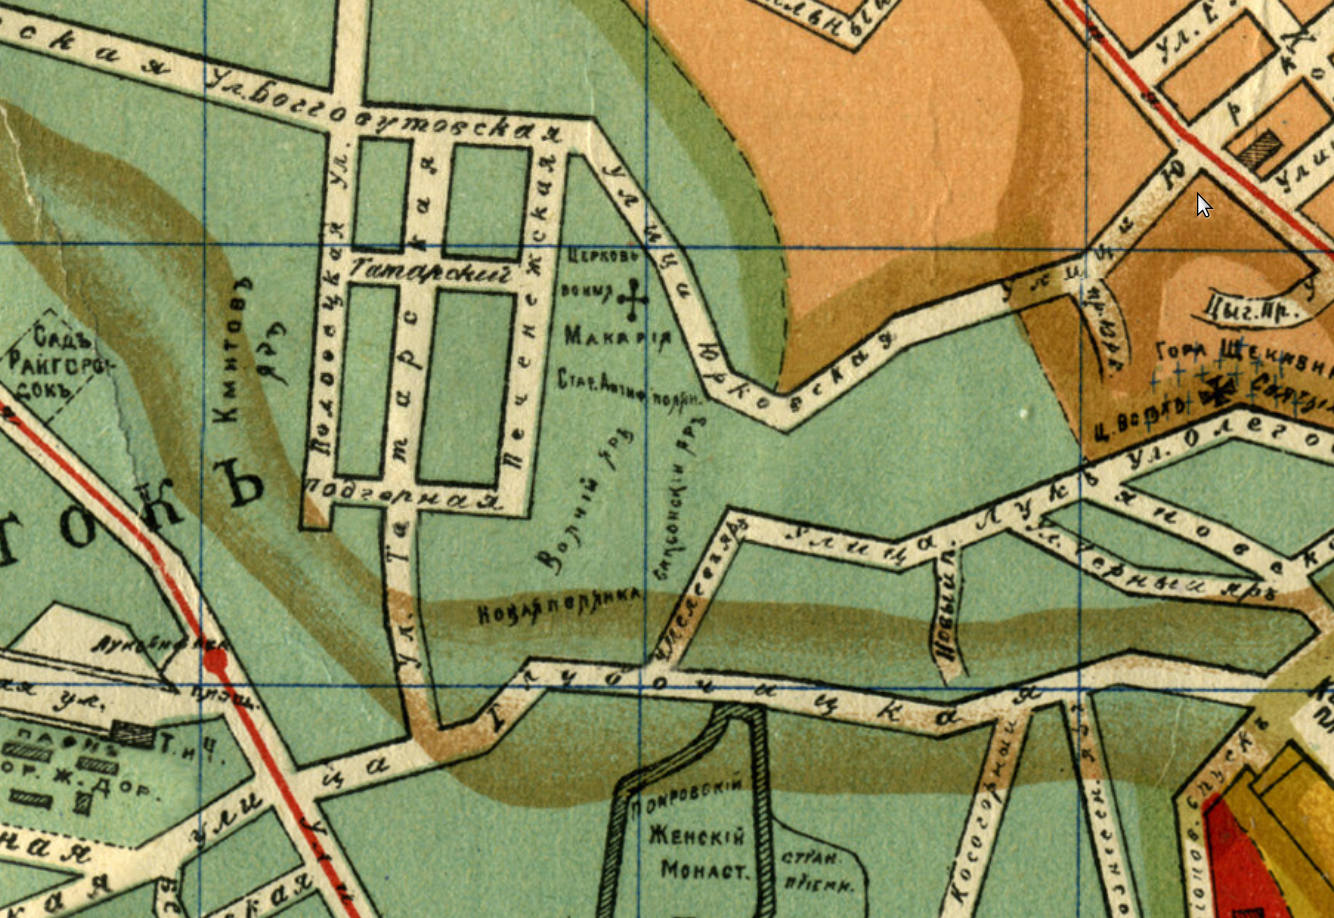
\includegraphics[width=\linewidth]{rpix/volch01.jpg}
\end{center}

На плане 1874 года Волчий яр как урочище лежит в районе нынешней улицы Лукьяновской между Чмелевым яром и Антифеевкой, и может быть отождествлен с Чмелёвым яром.

Выводы делайте сами, я не берусь. Добавлю также, что в начале 20 века на улице Волчий яр был трактир «Встреча хороших друзей».\\

\medskip

\textbf{Волчий яр} – по крайней мере, в середине 19 века так назывался овраг, в котором протекал ручей, известный ныне как Песочный (приток Лыбеди).

Яр начинался тремя приярками. Один брал начало возле современного северо-западного угла Пушкинского парка, около троллейбусного депо № 2 КП «Киевпасстранс» и дома на Дегтяревской 35/9, где было засыпанное ныне верховье яра.

Другой примерно где детская инфекционная больница на Дегтяревской 25. 

Третий от «дороги на Житомир», его сейчас во многих местах пересекает улица Зоологическая. 

В первом из приярков и начинался ручей Песочный (см. отдельную заметку о нем), но по сводному из трех приярков уже общему яру ручей протекал далее через нынешний Зоопарк и деревню Шулявщину (по месту улиц Шулявской, Ярмолы).\\

\medskip

\textbf{Вовчий яр} – на плане середины 19 века (увы, у меня только кусок его) так подписан «классический» Бабий яр в хорошо известных его пределах. Однако на той же карте, Бабьим яром подписана смежная местность, яр, начинавшийся в конце переулка Чаплыгина и через урочище Граевщину нисходящий к Сырцу в направлении Куренёвского кладбища. Либо, как вариант, яр на карте можно отождествить с улицей Ольжича.\\

\medskip

\textbf{Волчья гора} – возвышенность на Нивках между ул. Щербакова и железной дорогой на север от прудов на речке Сырце в парке Нивки идёт вверх крутой подъём. Улица Эстонская, застроенная частным сектором, прежде именовалась Волчьегорской.

Прежде у Волчьей горы был одноименный хутор, лежащий вдоль Волчьегорского шляха. Улица Эстонская занимает часть последнего.\\

\medskip

\textbf{Вольноживущевка} – окрестности переулка Балакирева на стыке Демиевки и Ширмы, именуется от прежнего названия переулка – переулок Вольноживущих.\\

\medskip

\textbf{Вознесенский яр} – глубокий яр между горой Воловней с ея Вознесенским спуском, и Кудрявцем. Сейчас по яру проходит улица Петровская (ранее Вознесенский яр), а исток яра, на юге, утопает в бурьянах и свалках на склоне, хотя еще в первой половине 20 века улица поднималась и присоединялась к Вознесенскому спуску, там где сейчас храм Василия Великого. 

Яр называется так от улицы, спуска, лежащего по его северному берегу, а спуск (в советское время улица Смирнова-Ласточкина) в свою очередь от Вознесенской церкви, которую в 19 веке снесли и поставили на нее месте либо здание духовной семинарии (ныне Академия искусств), либо южный корпус больницы Академии уже наук.

На южном берегу яра, по улице Кудрявской, над обрывом стоит дореволюционный дом номер 47, о трех этажах, причем с улицы видны только два и они обложены с фасада кирпичом, а вот если глядеть из яра, то дом трехэтажный и с той стороны два верхних обшиты темными от времени досками и дом кажется деревянным.

Берега яра – из суглинка, очень крутые, местами почти отвесные. На дне расположены автобаза и подобные объекты, а одной из террас, возле котельной – кинологический центр, откуда слышен хорош поставленный лай очень солидных, как оперные певцы, собак.\\

\medskip

\textbf{Выгода} – урочище, где на Виноградаре лежит озеро Синее. На стыке 19-20 веков соседствовало востоком с сыпучими песками. На плане 1923 года, Выгода протянулась нижней половиной вдоль урочища Сукачев яр, а верхней вдоль урочища Ветряные горы. И яр, и горы – к востоку от Выгоды.\\ 

\medskip

\textbf{Выдубичи} – древнее урочище, овраг в котором лежит Выдубицкий монастырь. С ним связано предание, что тут «выдыбнул» – прибился к берегу – свергнутый Владимиром с горы у Боричева языческий идол (не Перун, Перун поплыл к Днепровским порогам). Подробнее см. «Ересь о Киеве».

А вот метро «Выдубичи» названо так непонятно почему, ибо лежит между Бусовой и Лысой горами много южнее Выдубичей.\\

\medskip

\textbf{Высшая Лыбедь} – из справочника 1884 года: «сенокос площадью 24 десятины, на реке Лыбедь, у плотины при выезде от предместья Демиевки в город. Прежде здесь был Лыбедский пруд».

Из книги Похилевича "Монастыри и церкви Киева" 1865 года, владение Лавры, дававшее доход 270 рублей:

\begin{quotation}
Высшая-Лыбедь, бывший пруд с мельницею на Васильковской почтовой дороге. Плотина разорванная от грозового дождя в 1839 году, не возобновлена к поводу разногласия о том, кто должен содержать плотину, чрез которую проходит большой тракт. Ныне на месте пруда заведены огороды, пространством в 23 десятины, отдаваемые в аренду\footnote{Будущие Берлизовы огороды?}. 
\end{quotation}

\medskip

\textbf{Вумовский лес}

50°25'58.0"N 30°21'11.0"E

Лес со старыми могучими соснами и оврагом, в Петропавловской Борщаговке, в нем частично находится парк «Петропавловская Борщаговка». Лес расположен между частным сектором (что на берегу речки Борщовки) и промзоной. В лесу есть родник, выведенный трубой в озеро. На начало 21 века площадь леса составляла 13,4 га, с тех пор местность «осваивается» застройкой, на 2020 год осталось меньше половины.

Название происходит от ВУМ – Киевский завод Вычислительных и Управляющих машин, иначе говоря Электронмаш, который имеет адрес Окружная 4 и соседствует с лесом.\\

\medskip

\textbf{Высокое}

Урочище на Приорке, на плане середины 19 века обозначенное по координатам:

50°30'02.1"N 30°26'45.6"E

То есть к югу от Покровской церкви на Мостицкой улице. Церковь стоит на горбе, потом еще на северо-запад от церкви холм еще повышается, быть может название урочища относилось ко всей этой местности.  На той высокой части холма было прежде кладбище, а теперь небольшой парк с дубом на эдаком кургане. Остатки кладбища сохранились по другую сторону от церкви, да и между церковью и домом Мостицкая, 26 есть террасы\footnote{Кладбище сие было снесено в 1987 году.}.

А ниже церкви в то время стоял, на перекрестке, питейный дом – небось, чтобы нищие, получив под церковью милостыню, несли и пропивали там копеечку.\\

\medskip

\textbf{Вычовка} – см. Совка.\\
\chapter*{Г}
\addcontentsline{toc}{chapter}{Г}

\textbf{Галаганы, Станкозавод} – вплоть по середину 20 века, хутор примыкавший к юго-восточ\-ным околицам нынешней станции метро «Нивки». Теперь это местность окрестностей улицы Галагановской и от нее на восток и юго восток к Дружковской, к железной дороге.

Хутор в 19 веке основали братья Иван, Мусий и Егор Галаганы, что были лесниками.

В Галаганах было свое кладбище, сейчас там к северу от дома, что по адресу Галагановская, 6 – гаражный кооператив\footnote{50°27'24.1"N 30°24'15.2"E}. А на месте самого дома рос хуторской сад. Оттуда на восток протекал ручей, приток Рубежовского ручья, что и сейчас бежит течет вдоль железной дороги, дабы влиться в Сырец. Либо этот ручей можно считать одним из истоков Рубежовского. Другой исток находится у западного конца улицы Дружковской, там тоже гаражные кооперативы. Рубежовский впадает в Сырец около Рубежовской станции, там чуть ли не водопад, во всяком случае перепад высот внушительный.

Однако от северной части Галаганов, пересекая проспект Победы, у Сырца есть еще один приток – короткий ручей, что с пригорка впадает в Сырец к востоку\footnote{50°27'35.9"N 30°24'35.2"E} метрах в пятидесяти от первой гати через пруды в парке Нивки.

На хуторе Галаганы в 1893 году построили  церковь Святого Александра Невского (по проекту Владимира Николаевича Николаева). В росписи участвовали В. Васнецов, П. Сведомский, В. Котарбинский. Около церкви было кладбище. Храм закрыли в 1934, и уничтожили кладбище в 500 могил рядом с церковью. Ее помещение стало домом культуры Киевского завода станков автоматов. Вероятно, позже на его месте возвели новый ДК, имени Горького, а может это то же здание, переоборудованное. На 2021 год ДК Горького снесен, на его месте небоскреб.

От Станкозавода весь район Галаганы местные жители иногда так и называют – Станкозавод.\\

\medskip

\textbf{Гаращенко хутор} – см. Караваевщина.\\

\medskip

%Галерный остров (Водников)

\textbf{Генеральская дача} 

50°26'43"N 30°22'27"E

Дом отдыха высших военных чинов при воинской части А-3482, в северной части Казенного леса, на прудах одного из притоков речки Борщовки.

Южнее находится парк «урочище Совки», с селением Совки ничего общего не имеющий. Местных жителей на пруды не пускают. Только для людей в погонах!\\

\medskip

\textbf{Глинка}, озеро

50.409991399119036, 30.528935106396542

Водоем у западного подножия Черной горы, в ложбине, рядом с бульваром Дружбы народов. Это заполненный водой карьер кирпичного завода, частично совпадая со старым глинищем завода Эйсмана, позже Субботиной (дочь Эйсмана), еще позже Журавлева. В раскопах карьеров в окрестностях Глинки в 19 веке был найден янтарь, зубы акулы, древние следы растений – пальмы, секвойи, а также относящиеся к еще более давним временам морские растения. 

Глинка питается от родников, стекающих по склонам. На плане 19 века видно, что с северо-востока сюда стекал некий ручей.

Ложбина озера находилась прежде несколько западнее. Так на 1918 год, озеро размером с современное граничит строго с современным, но западнее, и еще западнее было два меньших озерца (а на север от них еще и озеро Бернер). Тогда же, на месте современного русла был склон горы. Подобное положение прослеживается по 1923 год, после чего, к 1930-му, два мелких озерца соединяются, а основной карьер начинает ползти на восток, поедая склон, но еще не заполняется водой.

На 1941 тогдашнее озеро Глинка уже наполовину совпадает с современным. По рассказам старожилов, туда во время войны со склона в воду съехал танк.

В начале нулевых мы со Светой Семёновой лазали по берегам озера в ходе съемок краеведческого фильма «Киевская сюита». На плоту по озеру плавали два пацана, мы стали расспрашивать их про озеро. Они поведали, что вроде бы на дне лежат машины, а также тут находили скелеты младенцев, потому что на другом берегу был роддом.

Роддома не было, но какие-то древние скелеты вполне могло вымыть водой из склонов, нарушенных добычей глины.

На склоне со стороны бульвара Дружбы Народов виднелся вход в дренажку. Берега были замусорены, со стороны переулка Филатова над озером нависала обрывом круча.

В конце 2016 года было затеяно укрепление берегов озера, сюда подвели какие-то трубы, сложившийся за десятилетия рельеф изменился бесповоротно. Еще весной 2016 года я успел вдоволь полазать по оползающим, частично превращенным в свалку, крутым и местами водоточивым и с рыжими железистыми частицами, берегам озера. Сверху же отлично обозревались окрестности в сторону Голосеево и Демиевки – высота огромная и всё видно как на ладони.

В 2019 году на берегах озера развернулись строительные работы по возведению ЖК.\\

\newpage

\textbf{Глубокий яр} – овраг на Черной горе, между улицами Тихая и Мендлеева. Занят гаражным кооперативом. В начале 20 века там был, вероятно, кирпичный завод Журавлева.\\

\medskip

\textbf{Глубокое, долина} – в 16 веке долина, описанная в документах как находящаяся между Кудрявцем и Лыбедью.\\

\medskip

\textbf{Глубочица, Глыбичица}, урочище

50°27'44.8"N 30°29'28.5"E

Окрестности низовий улицы Соляной и Пимоненко, да Кудрявского спуска = собственно тамошний овражище между горой Кудрявца и Щековицей.\\

\medskip


\textbf{Глубочица, Глыбочица} – взятая в коллектор речка, прежнее ее название – Кудрявец. Именно это название проходит в давних земельных документах и на картах. Например, на плане 1787 года русло Кудрявца в пределах Подола обозначено так: «канал чрез предместие из ручая Кудрявца». На карте же 1800 года название «Глыбiчица» приурочено к яру между холмом Кудрявца и Щекавицей, к средней его части (см. урочище Глубочица). На карте 1833 «Глубочица» подписан, насколько можно судить, отрезок оврага или речка в нем от Кмитова яра по нынешний перекресток Соляной и Глубочицкой, а на карте 1837 это уже определенно «речка Глубочица».

У речки два истока. 

Один начинается около Цветущего (Квитучего) переулка и стекает оттуда вдоль улицы Кмитов яр, где соединяется с истоком из другого отрога этого яра, что на территории Дачи Хрущова близ Института Педиатрии. О том, другом истоке читайте статьи Болото и Кмитов яр.

Миновав завод Артёма (в продолжении Кмитова яра на его нынешней территории был длинный пруд) Глубочица в подземном коллекторе пересекает улицу Татарскую и проходит в удолье меж двумя холмами до улицы Глубочицкой, через ЖК «Львовский квартал». До него там дичал пустырь, появившийся на месте разрушенного дрожжевого завода, что существовал кажется по крайней мере до конца 20 века. Завод сей возник на месте дореволюционного еще, водочного завода купчихи Чоколовой, а в удольи был большой пруд.

Другой пруд находился, по крайней мере в середине 19 века, в месте где сейчас улица Соляная соединяется с Глубочицкой. Ибо по оврагу Соляной тоже протекал крупный ручей, такой большой, что его можно считать третьим истоком Глубочицы.

Сейчас Глубочица принимает в себя несколько подземных ныне притоков, один из которых диггеры называют Кудрявцем, хотя без оснований, ибо Кудрявец это старое название самой Глубочицы. Этот приток, взятый в коллектор, начинается у сквера в самом верховье Кудрявского спуска, а затем идет под спуском до Глубочицкой улицы.

Другой приток, Киянка, выходит из урочища Кожемяки. Подробно я описываю всё это в «Ереси о Киеве» – что и где, и как Глубочица протекала в пределах Подола раньше. Здесь же добавлю, что Глубочица впадает в Киевскую гавань около Рыбальского моста.\\

\medskip

\textbf{Гнилая}, улица – улица старого, допожарного Подола\footnote{9 июля 1811 года сгорел почти весь Подол.}, шла примерно под нынешней улицей Боричев Ток. Послепожарная Гнилая – нынешняя Покровская.\\

\medskip

\textbf{Голгофа} – панорама, аттракцион, находился на Владимирской горке выше нынешнего Украинского дома, на уровне костела. Внутри павильона устанавливалась круговая картина и некоторые предметы, всё это составляло панораму. Первой темой ее были последние дни Христа, потом показывали «Вифлеем», «Поражение наполеона», «Распятие Христа».

Павильон открылся в 1902 году и был оснащен по последнего слову техники – для установки полотна картины применялась особая тележка на рельсах, темное время суток светили газовые горелки, в качестве материала для ступеней использовали модный тогда бетон. Голгофа обошлась предпринимателям-владельцам в 18 тысяч рублей, однако за два месяца они почти отбили эту сумму за счет посетителей.

Голгофа пережила революцию, множество смен власти и простояла на горке по 1934 год, продолжая приносить доход. За снос Голгофы ратовал режиссер Александр Довженко, коего избрали членом президиума Комитета содействия созданию парка и заместителем председателя проектного бюро. В 1934 году павильон разобрали, а полотно свернули в рулон и перевезли в Лавру, в успенский собор, где картина и сгинула вместе с собором в 1941 году.\\

\medskip

\textbf{Голосиевка}, совхоз – до пятидесятых годов 20 века лежал непосредственно к северу от большого пруда по нынешней улице Генерала Родимцева. Граничил с Покровской Голосеевской пустынью.\\

\medskip

\textbf{Гончары} – урочище между горами Детинкой и Старокиевской, проще говоря овраг с улицей Гончарной. Некогда тут жили гончары. В советское время на Гончарах стояли небольшие, о двух этажах кирпичные домики с садами. Тогда же местность слыла Гончаркой. Ныне урочище считают частью Воздвиженки.

Вообще прежде вся нынешняя Воздвиженка именовалась Гончары и Кожемяки, от смежных тут урочищ.\\

\medskip

\textbf{Горка} – короткий грунтовой путь по склону горы, на верхней террасе которой стоит дом по адресу Бастионная 11-А, а внизу – дом по Бастионной 13, он же Арсенальский. Если подниматься, то слева за гаражами и грушей-дичкой будет остаток частного сектора, длящийся до продолжения верхней террасы (уже под домом на Бастионном переулке, 11). Горкой пользуются в основном жители домов Бастионная 11-А и Бастионный переулок, 11. Первый из них тоже был ведомственный, построенный работниками (для них же) Полиграфкниги, ДОКа, и швейной фабрики.\\

\medskip

%Гостинец

\textbf{Город} – так жители Бастионной и окрестностей называли центр Киева вообще, а свой район не Зверинцем, а Печерском. Мы говорили: «Поехать в город», «Выберемся в город».\\

\medskip

\textbf{Госпитальное кладбище}, оно же военное. Дореволюционное. Остатки его находятся на южном краю Бусовой горы, в конце Зверинецкого переулка (бывшего Военно-Кладбищенско\-го). Лежало на месте склона Бусовой горы, изрядно съеденного добычей глины для кирпичных заводов, но вероятно зародилось не как военное, а как обыкновенное, еще в начале 19 века, поскольку на одной из могил сохранился год – 1812 и надпись, почему-то «МАНЯ».

В феврале 1878 года Киевское городское управление по просьбе Инженерного управления выделило тут землю, 4 десятины 2000 квадратных саженей под кладбище для военных, умиравших в госпитале. 

Еще в середине 20 века занимало всё низовье горы между железной дорогой, Зверинецким переулком, Соловцова, также в окрестностях улицы Сорочинской как к железной дороге, так и до Зверинецкой. Западным обрывом оно выходило к низовьям речки Бусловки, или, если угодно, к низовью улицы Киквидзе, там сейчас построили ЖК «Панорама». Теперь на месте большей части кладбище – частый сектор.

Смутно помню, что в 1990-х я, помимо креста с «Маней», видел там в зарослях конопли еще и могилы второй половины 20 века, вероятно местных жителей.

На кладбище установлен современный памятный крест в память воинов, погибших в ходе освободительной войны в Болгарии 1877-1878 годов.\\

\medskip

\textbf{Госпитальный спуск} – можно сказать, что бульвар Леси Украинки это сильно выпрямленный Госпитальный спуск. Тот шел примерно там же, но изгибаясь влево-вправо.\\

\medskip

\textbf{Государев сад}, позже Городской сад – заложен во время Петра I, занимал место, условно говоря, от Марьинского дворца по филармонию включительно, позже от него отчекрыжили, в северо-западной части, сад Купеческого собрания и Шато де Флер.

\medskip

\textbf{Граевщина} 

50°29'16.2"N 30°26'57.4"E

Так в 19 веке слыло большое, заросшее деревьями урочище на правом берегу речки Сырец, сейчас застроено разными ангарами. Напротив него на Сырце была плотина с городской мельницей, а выше её пруда, выше по течению – кожевенный завод купца Серебреникова, и выше его еще одна мельница на другом пруде. Но это отельный разговор, тогда вообще весь бедный трудяга Сырец был цепью прудов.\\

\medskip

\textbf{Графа Игнатьева} – урочище, слывущее на стыке 19-20 веков, оно же улица Большая на Верхней Соломенке. На Графе стояло тогда более 200 домов.\\

\medskip

\textbf{Графская гора} 

Условно говоря, склон над метро Крещатик, а шире – между улицами Городецкого и Круглоуниверситетской. Середина горы – улица Лютеранская, прежде Графская. На горе была Немецкая слобода.\\

\medskip

\textbf{Груша Володимирова} – урочище, в 16 веке граничащее с Тесными улицами и Старой дорогой.\\

\medskip

\textbf{Грушки}, хутор – по середину 20 века, хутор на одну улицу, между железной дорогой и началом (по перекресток с Выборгской) современной улицы Николая Василенко (и на восток от него). На восточных окраинах хутора было два жалких озера. Название хутора – от его прежних владельцев, дворянина Константина Грушко и его супруги Устины, владевших имением в 1871-1902 годах, после того как Киевская палата казенных имений выделила тут 14 земельных участков под аренду для киевлян, и Грушко взяли в свои руки большую часть. 

С 1898 по 1902 год земля (76 десятин) хутора отдана городом военно-инженерному ведомству взамен «военных» 38 десятин, отведенных под Политех.

По 1960-е в Грушках существовал частный сектор, застроенный позже промзоной.\\

\medskip

\textbf{Грушки} – район, промзона на месте бывшего хутора, ограниченная проспектом Победы, Гарматной, Машиностроительной, Василенко. Включает в себя жилой квартальчик Чугуевку\footnote{50°27'9"N 30°25'32"E}, получившую название от Чугуевского переулка. Там стоят хрущовки и двухэтажные домики. Зеленое тихое место.

\chapter*{Д}
\addcontentsline{toc}{chapter}{Д}


\textbf{Даронова гора} – на стыке 19 и 20 веков, так назывался склон между нынешним Олимпийским стадионом и Косым Капониром. Насколько я понимаю, Даронова гора – другое название Черепановой горы.\\

\medskip


\textbf{Далекий брод} – в середине 19 века, переезд на Лыбеди в районе около центрального вокзала, ниже впадения Скомороха, как урочище подписано на карте 1860 года на правой стороне Лыбеди, не доходя от устья Скомороха до Батыевой горы.\\

\medskip

\textbf{Дары} – бытовавшее по девяностые годы название известного овощного магазина «Дари ланів» на Бастионной, 1, на первом этаже. В 21 веке его помещение занимает то автосалон, то банк.

В советское время, рядом с «Дарами» слева располагался магазин «Трикотаж» с разными тканями, иголками, наперстками и готовой одеждой.\\

\medskip

\textbf{Дача Хрущова} – остатки жилой усадьбы в Кмитовом яру. В 1889 году тут купил участок земли Октавиан Бельский, помощник аптекаря. Спустя четыре года Бельский по проекту архитектора Николая Казанского начал строить тут особняк, а заимев уже собственную аптеку на Подоле, поставил рядом с особняком в Кмитовом яру доходный дом.

После революции местность, имевшую вид парка с двумя особняками, до тридцатых годов не трогали, ходили сюда все кому не лень, а потом обнесли забором и устроили жилье для номенклатуры. До 1937 года тут проживал Балицкий, нарком внутренних дел УССР. Потом его расстреляли, усадьбу отдали под пионерлагерь детей сотрудников НКВД.

В 1943 году место детей занял Хрущев, а когда он перебрался в Москву, «дача» осталась резиденцией первых секретарей ЦК. По слухам, под дачей был зал для заседаний и шел подземный ход со зданиями бывшей партийной школы. В 1978 году рядом построили Институт педиатрии, акушерства и гинекологии и усадьба вошла в его территорию.

В усадьбе дачи лежит мрачное верховье Кмитова яра с каскадом прудов, через которые перетекает ручей – один из истоков Глубочицы. Поверх переброшены мостики, или один мостик, не помню. Всё носит живописные следы разрушения. По дорожкам мамы катают в колясках детей.\\

\newpage

\textbf{Дача Хрущова} – другая, см. Васильчикова дача.\\

\medskip


\textbf{Дачная} – окрестности автостанции Дачная (проспект Победы, 142-А) близ Академгородка.\\

\medskip

\textbf{ДВС} – см. Водогон.\\

\medskip

\textbf{Дворцовый сад} – в 19 веке, название нынешнего Городского сада, там где стадион Динамо.\\

\medskip

\textbf{Девич-гора, Дивич-гора} – ныне, и примерно со второй половины 19 века известна как Лысая гора, та что ниже Зверинца. Упоминается в документах 16 века, как владение Михайловского монастыря – Дивич гора, земля Орининская, Орыновская.

Представляет собой большой, покрытый лис\-твенными деревьями и разнотравьем наверху холм с остатками Лысогорского форта. На Лысой горе растут и уничтожаются древние, возрастом много веков, дубы.\\

\medskip

\textbf{Дерперская роща} – на середину 19 века занимала Кристерову горку и окрестности. Занимала местность от нынешней Кристеровой горки (что к северу от улицы Осипова) и на юг к ручью Коноплянке и прудам на оном. В роще находился хутор графа Эстерази, как раз где сейчас известен старинный дом Кристера. До Эстерази, там был хутор Дерпера, от чего и пошло название.\\

\medskip

\textbf{Дехтяги, Дегтяри} – район между Нивками и Галаганами, частный сектор по улице Януша Корчака от улицы Эстонской до Краснодарской. Еще в 1940-х считался хутором. Хутор был основан крестьянином села Беличи, Василием Дехтяренко. Между домами номер 22 и 28 по улице Ставропольской, а точнее в Ставропольском переулке, есть маленькое, но старое кладбище\footnote{50°27'56.7"N 30°24'46.3"E}. В 1970 году останки с кладбища перенесли на Берковецкое, в 1980-х здесь устроили спортивную площадку, но там никто из местных не играл, ибо знали, что это место кладбища. На 2021 год – заросший травой пустырь. Окрестности кладбища и есть исторический центр Дегтярей. В районе Нивок проживает много людей с Фамилией Дехтягенко.\\

\medskip
%В 1876 году Григорий Галаган отдал в Дегтярях усадьбу, под ремесленное училище. 

\textbf{Дегтяры} – урочище в овраге между горами Валовой и Детинкой, там где улица Дегтярная. Плотно застроен новыми домами, которые путают с близлежащим кварталом Воздвиженкой, названным так по Воздвиженской улице и занявшим урочища Гончары и Кожемяки. 

Можно сказать, что Дегтяри это часть урочища Кожемяки, делящая с ним одно отпочкование оврага. Основные Кожемяки – между Воловней и Замковой. Часть Кожемяк заходит в овраг между Воловней и Детинкой, у склона Воловни. В то же время Дегтяри – параллельны этой части Кожемяк, но у склона Детинки.\\

\medskip

\textbf{Деловой двор} – существовал в 19 веке, отсюда и Деловая улица. Стоял на перекрестке Деловой и нынешней Большой Васильковской (Красноармейской).\\

\medskip

\textbf{Детинка, Дытынка} 

50°27'31.7"N 30°30'42.2"E

%Гора на север от БЖ, эдакий длинный отрог, что лежит между Клинцом, Замковой, Валовой и Старокиевской горами, или, если угодно, между ярами-урочищами Дегтяры и Гончары (улица Дегтярная и Гончарная). Крыши строек по обе стороны Детинки вровень с плато самой горы. Она имеет любопытный, удобный для обороны вид сверху – толстое основание у материка, затем узкий перешеек, затем расширение, как бы голова. Достаточно охранять перешеек малыми силами.

Гора на север от БЖ, эдакий длинный отрог, что лежит между Клинцом, Замковой, Валовой и Старокиевской горами, или, если угодно, между ярами-урочищами Гончары и Кожемяки. Сейчас различие размылось, а прежде Кожемяки были к  западу от Детинки, а Гончары на север и восток. Там же выделяли еще урочище Дегтяры, и есть улица Дегтярная.

Крыши строек и новстроек по обе стороны Детинки вровень с плато самой горы. Она имеет любопытный, удобный для обороны вид сверху – толстое основание у материка, затем узкий перешеек, затем расширение, как бы голова. Достаточно охранять перешеек малыми силами.

Склоны из суглинка, заросли травой и деревьями. Самая северная часть отрога – лысая. По верху всей горы идет тропа от Пейзажной аллеи (БЖ).\\ 

\newpage

\textbf{Дидоровка}
 
50°22'32"N 30°30'9"E

Удольный пруд в Голосеево, к южной стороне водоема примыкает очень высокая гора с лыжной трассой, а берега оборудованы избушками для пикников, за сидение в избушках берется плата. К Дидоровке добираются по горной дороге от Сельхозакадемии, что пролегает прямо через ботанический сад, мимо Голосеевской пустыни.

В первой половине 20 века, Дидоровка относилась к лежащим от нее на сервер землям совхоза Голосиевка, что был по дороге к Покровскому Голосеевскому монастырю (пустыни).\\

\medskip

\textbf{Диск} – парк в Корчеватом. Назван так по одноименному кинотеатру, развалины коего еще виднеются.\\

\medskip

\textbf{Дниструиха}, озеро

См. Корчи.\\

\medskip

\textbf{Довнар} – улица Довнар-Запольского и окре\-стности, от Ванды Василевской до Лукьяши. По адресам 1/12, 3/1, 3/2, 4 лежит микрорайон домов в стиле конструктивизма, построенный в 1920-30-х (чего по ним не скажешь), по проекту архитектора Михаила Аничкина. Часть домов «конструктивистского» микрорайона относится к улице Коперника – номера 20, 18.\\

\medskip

\textbf{Дом Гинсбурга} – первый киевский небоскреб в 11 этажей, стоял на холме чуть севернее нынешней гостиницы «Украина» на Институтской улице – через улицу напротив южного крыла Института благородных девиц. Короче говоря, там где сейчас автостоянка перед гостиницей. 

Построен в 1910-12 годах по проекту архитекторов Адольфа Минкуса и Фёдора Троупянского. Строителем и владельцем был купец первой гильдии Лев Борисович Гинсбург. Стоимость здания оценивалась в полтора миллиона рублей. На постройку ушло 12 миллионов кирпичей. 

Высота каждого этажа равнялась 4 метрам, здание венчала башня в 10 метров. Дом после постройки использовался как гостиница и под сдачу квартир. В 1917 году, аренда в нем квартиры на год стоила 1300-1700 рублей. Сам Гинсбург жил в двухэтажном особняке неподалеку.

После революции дом Гинсбурга национализировали и превратили в коммуналку. В 1941 году в нем квартировал Иван Кудря, хранивший там свои документы для «легенды» и прочие важные в подпольной деятельности вещи, и когда небоскреб вместе с многими другими зданиями на Крещатика был взорван в 24 сентября 1941 года – раньше писали, что немцами, нынче пишут, что нашими.
 
В Киеве на улице Городецкого, 9 есть еще один «дом Гинсбурга», поменьше, тоже был доходный дом – роскошный, украшенный скульптурами. Он тоже пострадал во время взрыва, лишившись трех башенок. Стоит рядом с кинотеатром «Украина».\\

\medskip


\textbf{Дом Понятовского}

%https://ru.wikipedia.org/wiki/%D0%9A%D0%B8%D0%B5%D0%B2%D1%81%D0%BA%D0%BE%D0%B5_%D0%B4%D0%B2%D0%BE%D1%80%D1%8F%D0%BD%D1%81%D0%BA%D0%BE%D0%B5_%D1%81%D0%BE%D0%B1%D1%80%D0%B0%D0%BD%D0%B8%D0%B5
%Маврикием Понятовским по проекту А. В. Беретти. Г

Не сохранился, снесен в 1976 году. Помещик, камергер Ламберт-Маврикий Понятовский\footnote{Усадьба была куплена его отцом, полковником Иосифом Понятовским, в 1828 году.} в 1851 году возвел, несколько не доведя строительство до конца, кирпичный трехэтажный дом примерно по месту северного пересечения Майдана и Крещатика\footnote{50.450560, 30.524440}, по несколько переделанному в Петербурге проекту киевского городского архитектора Людвига Станзани.

Газета «Киевские епархиальные ведомости» писала:

\begin{quotation}
Дом этот представлял собой в середине ХІХ в. наглухо забитую безлюдную постройку. Как это вышло? Дом строил польский магнат Понятовский. Этому вельможе какой-то ксёндз навеял, что с завершением постройки он умрет. Перепуганный вельможа прекратил сооружение своего дворца, забил окна и двери и дом превратил в такое легендарное здание. В конце 1850-х годов с этого дома сняли темную легенду, оживили его, открыли окна и двери. Тут была устроена художественная выставка.\end{quotation}

Затем на первом этаже Понятовский сдавал помещения под магазины, а в 1861 году продал здание Дворянское депутатскому собранию Киевской губернии.

Прежде чем я продолжу о судьбе здания, проследим судьбу Понятовского. Он умер 8 мая 1878 года в другом своем доме, на Липках. Вдова Понятовского заказала жившему в Риме скульптору Бродскому за 30000 франков мраморную сидячую статую покойного. В 1882-м Понятовская намеревалась поставить оную статую в Александровском костеле, близ престола, как бы уравнивая усопшего мужа со святыми, но духовенство не поддержало начинание. Что до самого Понятовского, то могила его поныне есть на Байковом...

Итак, дом Понятовского стал домом Дворянского собрания, где оно собственно сходилось на собрания, устраивало маскарады, концерты и выставки, а в 1865 году там в трех комнатах была устроена, хотя через несколько лет переехала, еще и Публичная библиотека Киева. В 1895 году Собрание сдало часть своей усадьбы в аренду Киевскому обществу взаимного кредита, и то пристроило своё здание, фасадом подобное бывшему дому Понятовского. 

После революции 1917 года в здании Собрания, на Крещатике 16, поместилась военная комендатура – то немцев, то красных – первым советским комендантом города было Щорс. Затем здание стало Домом работников просвещения, потом Домом учителя, хотя на первом этаже продолжали располагаться разные магазины.

Еще позже там расположились цеха типографского предприятия Полиграфкнига, и в них работала моя бабушка, Татьяна Федоровна Бородина.

Наконец на том же углу появился Дом Профсоюзов...\\

\medskip

%\textbf{Дом с ирисами}
%https://kyivcity.net/kiev/dom-s-irisami-v-kieve-gde-naxoditsya-pochemu-tak-nazyvaetsya-i-v-kakom-on-sostoyanii-foto/
%\medskip

\textbf{Дом Рыбальского}

50°27'48"N  30°30'53"E

Адрес: ул. Никольско-Притисская, 5

В этом доме, примыкающем к Флоровскому монастырю, проживал Георгий Рыбальский, бывший киевским войтом в 1797-1813 годах. Само одноэтажное здание, кажется, построено еще раньше. В нем был подвальный этаж.

Дом пережил подольский пожар 1811 года, а когда в 1813 году Рыбальский умер, дом унаследовали потомки. В 1857 году здание перекупили и сделали рядом двухэтажную пристройку – она больше первичного дома и уходит как бы вглубь Флоровского монастыря.

Если стоять лицом к дому, то справа будут ворота, а еще правее них еще один одноэтажный дом, тоже под номером 5. Так вот дом Рыбальского – только «левый», тот, что расположен дальше от входа в монастырь.

Глядя на этот по нынешним меркам небогатый, в пять окон, домик, на ум приходят несколько мыслей. Либо войт Рыбальский был скромен, либо тогда остальные жили много хуже. Или же у людей были другие потребности.\\

\medskip

\textbf{Дом старой почты} – местное название трехэтажного, 1951 года постройки дома по Татарской 32-Б. Раньше там, на первом этаже, была почта, а еще прежде – конюшня, клуб, кинотеатр.

В бытность там почты, оная использовалась как «здание гестапо» в фильме «Нина» о киевских подпольщиках, семье Сосниных.\\

\medskip

\textbf{ДОК}

50°24'24"N 30°34'36"E

Дерево-обрабатывающий комбинат, расположен в промзоне Теличке. Рабочих его называли «доковцами». На 2021 год, в части корпусов расположились другие фирмы. К заводу подходит улица Деревообрабатывающая.\\

\medskip

\textbf{Дом Самолёт} – дом справа от станции метро «Арсенальная». Построен в 1930-х по плану Каракиса.\\

\medskip

\textbf{Древлянская площадь} – во второй половине 19, начале 20 веков – площадь у перекрестка нынешних улиц Дегтярёвской, Якира и Зоологической. Неподалеку площади начинал по поверхности течь ручей Скоморох. А по другую сторону от площади и Старожитомирской дороги (ныне Дегтярёвская), близ западной стороны площади, по 1880-е располагался ипподром.\\

\newpage

\textbf{Дружбы} – станция метро Дружбы Народов, одновременно народное сокращенное именование бульвара.\\

\medskip

\textbf{Душегубица} – на плане Ушакова 1695 года, Наводницкий овраг обозначен как «боярак Душегубица». А вдруг это искаженное упоминание «дороги на Выдубичи», как обычно подписано примерно там на других, хотя и более позднейших картах? Однако, в письменной росписи на том же плане Ушакова, сказано:

\begin{quotation}
С Киевской стороны до реки Лыбеди около посаду от горы, что подле Николаевского монастыря до бояраку, прозываемом Душегубицы, 855 сажень, в том числе на 345 саженях валок, старинной небольшой [...]\end{quotation}

И далее Душегубица еще упомянута дважды, и что от Душегубицы «большими лесами меж гор к реке непрву 924 сажень».\\

\medskip

\textbf{Дымерский шлях} – давняя дорога из Киева через Межигорье, Вышгород, затем в Дымер и Чернобыль.

%Дурка
\chapter*{Е}
\addcontentsline{toc}{chapter}{Е}

\textbf{Евбаз} – Еврейский, или Галицкий базар, что был на площади Победы, там где цирк. На Евбазе стояла настоящая Железная церковь. В конце 1940-х общенародную барахолку ликвидировали, снеся сараи складов и ларьки. В 1952 году освободившуюся Галицкую площадь переименовали в площадь Победы.

В восьмидесятые-девяностые Евбазом называли уже небольшую толкучку около трамвайной остановки рядом с универмагом Украина.\\

\textbf{Еврейское кладбище} – кроме того, что с 1798 года было на Зверинце\footnote{Т.н. Старое еврейское кладбище, на его месте ныне участок вьющихся растений в ботсаду. В 1895 году объявлено закрытым.}, существовало еще одно иудейское кладбище, и находилось оно не по месту нынешней телевышки (там было Братское), а почти рядом, по другую сторону улицы Мельникова, правее спорткомплекса «Авангард» (построен на месте мусульманского и караимского кладбищ). От еврейского кладбища осталась его бывшая контора, двухэтажный дом по адресу Мельникова, 44. Здание телецентра рядом – Карандаш – стоит на месте еврейского же кладбища.\\

\textbf{Евсейкова долина} – урочище, упоминаемое в земельных документах 16-18 веков. В грамоте Жикгимонта I, разрешающей восстановить Михайловский Златоверхий монастырь, 15 марта 1523 года, описываются границы принадлежащей монастырю земли в Киеве:

\begin{quotation}
и земли к тому манастырю мает держати по давному, как перед тым бывало, по самый вал, и по Лядскии ворота, и по Евсийкову долину, по старую дорогу, по Михайловский ввоз.
\end{quotation}

В высочайшем Е. И. В. указе из прав. сената от 13 декабря 745 г. за № 9490, написано: 

\begin{quotation}
в прав. сенате Киево-золотоверхо-михайловского мн-ря архимандрит Си\-львестр Думницкий с братиею бил челом, объявляя, что на данную от доброхотнодателей, лежачую за старокиевскою крепостию, в даче по урочищам от долины Евсейковой, землю со всем, которая сошлась того места к берегу реки Почайны, крещацким взвозом в 1700 году блаженныя и вечнодостойныя памяти государь император Петр Великий, жалованною грамотою, по королевским привилегиям, в вечное и ненарушимое владение мн-рю Михайловскому всемилостивейше ствердил и укрепил. 

и по оной грамоте для варения в мн-рь меду, пив и прочаго, провар в 1745 году на оной крещатицкой земле начато строить, ибо в мн-ре провапа, воскобойни и винокурни за немалым в том мн-ре утеснением и за хоромным деревянными многим строением, а наипаче за великим от огня страхом содержать опасно [...]
\end{quotation}

Вероятно, Евсейкова долина это давнее название удолья, где лежит улица Крещатик.\\

\chapter*{Ж}
\addcontentsline{toc}{chapter}{Ж}

\textbf{Жаба}

50°27'19.2"N 30°31'45.4"E

Знаменитая в советское время танцплощадка, что была на склоне между лестницей, ведущей к памятнику Магдебургскому праву, и Аркой в честь воссоединения Украины с Россией. Просуществовала в относительно целом состоянии  примерно по 2012 год. Название возникло от скульптуры зеленой жабы (метр на полтора), стоящей неподалеку.

Над танцплощадкой Жабой раньше был ресторан Слоник, названный так от фонтана со скульптурой слона.\\

\textbf{Жандармский сад} 

В. Л. Беренштам в «Т. Г. Шевченко и простолюдины, его знакомцы» писал в 1900 году:

\begin{quotation}
В течение года я еще раза два встречал Чапыгу: мои знакомые видели его не раз на народных гуляниях, а также на вечерах в Жандармском саду (сад находился там, где теперь Николаевская, Ольгинская и Меринговская улицы);
\end{quotation}

\textbf{Желань} – летописное урочище, возможно нынешние Жуляны, вопреки расположению улицы Жилянской. В 1161 году Торки, преследуя Изяслава от Белгорода (современная Белогородка), настигла обоз Изяслава у Желани, а его полки – около Буличей (Беличей). Вероятно с Желанью корнем связана и Шулявка (и летописный Шелвов борок). Расстояние между Жулянами и Шулявкой всего 5 километров.\\ 

\textbf{Жеребьевщина}

50°30'03.2"N 30°25'57.3"E

На середину 19 века урочище представляло собой прямую улицу, вдоль которой стояли домики с большими садами. Ныне - многоэтажная застройка, дома 6 и 12 в Апрельском переулке.


В начале 20 века урочище с юга огибала Жеребьевская улица, ныне Новомостицкая.\\


\textbf{Жилгородок} – район на Бусовой горе, между низовьями улицы Зверинецкой (от дома 61) и параллельном ей там же отрезке Бусловской, по улицу Соловцова. Естественная застройка советского времени – хрущовки в 3-5 этажей, и пара девятиэтажек. В Жилгородке обитали рабочие ДОКа, знавшие друг друга в лицо, а окружающая местность представляла собой частный сектор. Ныне частный сектор преобразился в терема, а частично застроен небоскребами ЖК Триумф и Бусов Хилл. Исчезла также двухэтажная общага серии 207-7 на Бусловской, 15. За нее, справа, спускались быстрым путем на Тимирязевскую (мимо дома 42 на оной).

В советское время в Жилгородок ходило ма\-ршрутное такси – небольшой автобусик – от разворота за Печерским мостом (ближе к Суворовскому училищу), и в Жилгородке около трехэтажки по адресу Зверинецкая, 32 (с продуктовым магазином на первом этаже) была другая его конечная. Название Жилгородок – чисто местное – я, живя на близлежащей Бастионной, его не слышал (а узнал о нем только в 2017 году от Entertaining stuff with eng subs), хотя в нашем доме на Бастионной жили в том числе и доковцы.\\

\textbf{Жуковка}, лаврский хутор 19 века – от него название Жукова острова. При хуторе было урочище Чернечье, оно же Галерное.\\

\chapter*{З}
\addcontentsline{toc}{chapter}{З}

\textbf{Забора, Забара} – урочище, известное в 19 века, перекресток нынешних Автозаводской и Луговой, еще тогда это был перекресток дорог. Через него, чуть южнее, с Приорки протекал ручей Западинка.

От названия местности происходили улицы Старозабарская (часть ее стала Автозаводской, часть исчезла в 1980-х вместе со сносом старой застройки) и параллельная ей Новозабарская.\\

\medskip

\textbf{Забара} – на плане окрестностей Киева 1850 года так обозначено некое урочище южнее Братской Борщаговки, между нею и северо-западной окраиной Жулян.\\

\medskip

\textbf{Загоровщина, Загоровка, Загара}

50°28'26.3"N 30°29'07.7"E

Местность на Татарке, заросшие деревьями и кустами склоны Кирилловских высот условно напротив Института автоматики на улице Нагорной. На начало 21 века у местных жителей в ходу название Загоровка, туда на террасу-площадку за зданиями ходят устраивать пикники. Площадка слывет как Загара или Нижняя стрелка, Стрельбище либо Кафе Прощай Молодость, из-за встреч там одноклассников.

Стрельбищем площадка именовалась от того, что там было стрельбище вышележащего по склону гостинично-спортивного комплекса «Авангард» (его построили к Олимпиаде 1980 года). Поныне земля усеяна там, около забора, разбитыми тарелочками вроде виниловых, используемых в качестве бросаемых в воздух мишеней.

Загоровщина известна по делу Бейлиса как место нахождения в пещере трупа мальчика Андрея Ющинского. Урочище простирается по Смородинский спуск включительно.

Вообще говоря, пещер на Загоровщине было много, как и на близлежащем Смородинском спуске. Но сейчас на Загоровщине пещеры, судя по всему, все засыпаны.

В начале лета 1831 года мещанин Василий Ювженко обнаружил где-то на Загоровщине, под липой, пещеру глубиной более 2.8 метра, которую позже засыпали. 

Я не знаю, почему на современных картах урочище Загоровщина обозначена в районе улиц Пугачева и Герцена, то бишь верховья Репяхова яра. Вероятно именно с карт оно стало проникать и дальше. Предположу, что корень сего мнения о расположении Загоровщины лежит в топонимическом словаре Резника и Пономаренко.\\

\medskip

\textbf{Замковище} – урочище южнее Мостицкого массива и горы Липинки, в районе улицы Замковецкой и Замковецкого переулка. На начало 21 века там частный сектор и застраиваемая местность. Название дает основание полагать, что здесь были остатки какого-то замка. Соседствует с урочищем Беличье поле.\\

\medskip

\textbf{Замок Ричарда Львиное Сердце, Дом Ричарда} – дом на Андреевском спуске, 15, назван так по внешнему виду, напоминающему замок (раньше там была еще винтовая лестница) и жильцу по имени Ричард Матвеевич Юревич, который обитал там по крайней мере по 1970-е. Юревич некогда был уланом польской армии и воевал в Первой мировой. Знал семью Булгаковых, живших чуть ниже в 13-м доме. На первом этаже Замка Ричарда раньше была, кроме прочего, конюшня.

Построенное в начале 20 века на средства купца Орлова, здание было доходным домом, после революции в нем разместились коммунальные квартиры. Предание гласит, что вдова Орлова расплатилась со строителями несправедливо, и те «поселили» в дом привидений, насыпав в дымоход яичную скорлупу. Её нашел там профессор Киевской Духовной академии Степан Тимофеевич Голубев и объяснил, что воздух, проходя через мелкие дырочки в скорлупе, вызывал те странные
звуки, что пугали обитателей дома и создавали оному дурную славу.

Дом западом выходит к небольшой горе Уздыхальнице с плоской, срезанной верхушкой – с верхушки есть один из входов в Дом Ричарда. И у северного подножия этой горы – «дом Булгаковых».\\ 

\medskip

\textbf{Западинка, Западинский}, ручей – протекал большей частью в длинном овраге, где сейчас проспект Правды. Овраг начинался у перекрестка проспекта Правды с Межевой.
 
Название ручья происходит от местности Западинка (Западинцы). 

От прежнего частного сектора осталось две улицы – начало Западинской и Галицкая (бывшая Песчаная или Песочная). Песочная лежала выше, севернее ручья. На карте Кульженко 1894 года, по северной стороне улицы Песочной, вдоль нее и до перекрестка с Вышгородской показан короткий ручей, невесть куда впадающий.

Сам же Западинка протекала так – по ходу нынешнего проспекта Правды, по нынешней улице Ивашкевича до перехода ее в улицу Луговую, где сворачивала более на юг, следуя на запад от улицы Автозаводской (прежней Старозабарской) до соединения с Курячим Бродом, и далее общий поток шел в речку Сырец.

Некоторые диггеры имеют иное мнение про ручей Западинку, называя так ручей, что течет под Геофизприбором и улицей Западинской к Вышгородской, и затем прослеживают ход сего ручья под улицей Полупанова (ныне Приорской) и к Бережанскому рынку. Очевидно, что речь идет о безымянном ручье, что протекал вдоль Песочной улицы. Однако, возле перекрестка с Вышгородской к коллектору этого ручья присоединяется коллектор, проложенный под проспектом Правды – истинное русло Западинки.\\

\medskip
%чинается под гаражами на улице Новомостицой, затем идет южнее Брестской (параллельно ей) через местность Замковище, всё более застраиваемую высотками вместо частного сектора. В Замковище еще в 19 веке были остатки какого-то замка.\\

\textbf{Западинцы, Западинка}

50°30'20.0"N 30°25'57.0"E

Гора, урочище – холм на север от проспекта Правды, бывшего оврага, где протекала речка Западинка. На карте середины 19 века гора Западинка лежит между проспектом Правды, проспектом Свободы и Межевой улицей

%По урочищу лежала улица Лысогорская, эдак от Западинской к нынешнему проспекту Победы. На Западнике была своя Лысая гора.

По ряду старинных карт, урочище Западинцы занимает оба берега оврага проспекта Победы, и северный и южный.

Севернее располагается местная Лысая гора, никем уже не угадываемая.\\

\medskip

\textbf{Запечерка, Запещерка} – местность за Лаврой, там где сейчас музей Великой Отечественной Войны. Улица Запещерная, прежде проходящая через частный сектор, существует и сейчас в виде безымянной дороги к музею, отходящей на гору от улицы Лаврской. Там же были улицы Запещерная-Лабораторная, Ново-Петровская, а участок Лаврской снизу доверху назывался прежде Ново-Наводницкой.

В справочнике Пономаренко и Резника упоминается «народное название» этой местности – Запретка, которое лично я не слышал, и оно напоминает мне искаженную Запещерку. Справочник же производит «Запретку» от неких бывших тут языческих капищ, дескать, место было запретным для нечистой силы. Хотелось бы знать источники, откуда сие почерпнули сочинители справочника.\\

\medskip

\textbf{Запольская дорога} – известная по крайней мере в 18 веке дорога, она же Великая, шла через Вету, как и Белоцерковская, а от Веты отделялась через Юровку к городам Запольским, Заполью в Невеселовском поле над Унавой, Ирпенем и Стугной.\\

\medskip

\textbf{Зверинец Неводничий} – отдельное урочище на Зверинце, принадлежал Выдубицкому монастырю, упоминается с начала 17 века.\\

\medskip

\textbf{Звенигород} – согласно Нестору, «иже есть город мал у Киева, яко десяти веръсты въдале». По ряду списков, однако, не Звенигород, а Белгород.\\

\medskip

\textbf{Зелёнка}

Сам театр: 50°26'49"N 30°32'47"E

Верх. опорн. стена: 50°26'49"N 30°32'46"E

Нижн. опорн. стена: 50°26'52"N 30°32'49"E

В середине 19 века, в связи с сооружением Цепного моста и прикрывавшей его башни – Подольского набережного верка – на склоне над Днепром соорудили две полукруглые подпорные стены, под которыми проложили тоннели трубопровода водокачки Подольского верка. Водокачка находилась в верке, и по чугунным трубам вода из Днепра поступала в мастерские Арсенала, соединенные с верком подземным ходом. 

Подземные коридоры остались поныне. 

На нижней стене тренируются альпинисты и скалолазы. Если подняться по земляной горе к верху опорной стены, слева будет вход в стену – темный кирпичный провал ведет в коридор, где разбитая, опасная лестница сходит вниз. По правую руку – бойницы, сужающиеся наружу. Я не спустился в самый низ из-за того, что фонарик разрядился, а света фонарика в смартфоне было мало. Пол внизу усыпан битым кирпичом, и если ход есть, то между полом и потолком расстояние теперь совсем невелико и с лестницы его нельзя определить. Всё очень загажено. 

Если идти к нижней опорной стене со стороны Днепра, шоссе, то не доходя до нее, слева\footnote{ 50°26'52"N 30°32'52"E}, будет круглый вход в дренажку ЗТСМД («Зелёный театр – станция метро Днепр»), куда можно войти чуть пригнувшись. На лето 2021 вход открыт. По середине бетонной трубы течет водный поток, идти первые несколько метров можно еще по краю, а потом нужны резиновые сапоги или бахилы.

Неподалеку, но выше, над нижней стеной, есть также популярная среди диггеров ДШС №12 (50°26'52"N 30°32'48"E).

В 1949 году по проекту архитекторов А. Власова и А. Заварова и инженера Н. Пестрякова между подпорными стенами был построен Зеленый театр на 4000 мест, использовавшийся в том числе как кинотеатр под открытым небом.

Его-то развалины и были в 1990-е облюбованы неформалами и среди нефоров Зелёнкой слыли именно остатки зеленого кинотеатра. Там зарождалось диггерское движение, а про окрестности ходили слухи и страшилки, что это аномальная зона с подземными порталами куда-то. И дескать, по Зелёнке бродит потустороннее существо – Хозяин.\\

%РАСШИРИТЬ!!!!

\medskip

\textbf{Зелёнка}

50°27'38"N 30°24'29"E

Зеленый театр в парке «Нивки». Построен в 1958 году как летний, на 2700 мест, кинотеатр «Ленинского комсомола» (одноименный с этой частью парка), по проекту архитектора Чуприны.

На 2021 год закрыт и пребывает в плачевном состоянии.\\

\medskip

\textbf{Зорька} – советский кафе-бар «Зоряне», близ кинотеатра «Украина» на улице Карла Маркса.\\
\chapter*{И}
\addcontentsline{toc}{chapter}{И}


\textbf{Ивницкий гостинец} – давняя дорога, она же Старое путище, дорога Киевская, Смоляная, Смолянская. Лежала из Киева через Лыбедь, Борщаговку, Белгородку в Ивницу и на Волынь (цитирую Руликовского «Повет Васильковский»).\\ 

\textbf{Иорданские рогатки} – бытовавшее в 19 веке название места вокруг нынешнего перекрестка улиц Нижнеюрковской и Нижнеюрковского переулка.\\

\textbf{Исаев хутор} – на стыке 18-19 веков, хутор в удольи близ южного склона Девич-горы (Лысой).\\

\textbf{Итальянский домик} – одно из названий облезлого, розово-бежевого жилого дома работников обувной фабрики № 4. После войны его реконструировали пленные итальянцы. Находится на Приорке, по адресу Сокальская улица, 1. Построен по проекту архитектора Каракиса в 1940–1941 годах. 

После войны там жили «водники» (детский сад водников стоит рядом, занимая двухэтажное старое здание), затем дали квартиры еще и пожарникам, после чего дом стали называть Пожаркой.

Лестницы в доме расположены по бокам, от лестниц отходят внешние, открытые галереи, с которых и можно попасть в квартиры. Дом четырехэтажный, с колоннами, которые как бы защищают галереи. В доме 50 квартир, на 1 и 2 комнаты, потолки высокие.

Рядом, по той же стороне улицы, двухэтажные дома, с виду тех же годов.

Большую часть сведений о доме я получил от Даши Кононюк, пытаясь поначалу уточнить – верно ли, что местные именуют этот домик Китайкой. Оказалось, что нет.\\

\textbf{Ицун, Вицун} – в 17 веке рукав Днепра, в начале 20 уже озеро. Один из потоков, питавших верховье Почайны.

\chapter*{К}
\addcontentsline{toc}{chapter}{К}

\textbf{Кадетская роща} – не путать с улицей Кадетский гай в Турецком городке. Непонятно, почему так назвали улицу, лежащую много в стороне от Кадетской рощи.

Кадетская роща, вернее её остатки, лежат на склоне горы вдоль Лыбеди, между Чоколовским бульваром, Уманской улицей и улицей Железнодорожной (а затем рельсами Оборотного парка Киева-пассажирского). На карте Шуберта роща обозначена как Кадетский бор.

Официально ее именуют сейчас «парк Спутник».

Сейчас размер Кадетской рощи составляет, на глазок, 15 процентов от ее площади по карте 1842 года, когда роща покрывала нынешний Первомайский массив и часть Кардач. Но и современные остатки рощи сопоставимы с ботсадом имени Фомина, что в центре. И эти остатки теснятся гаражными кооперативами, культовыми сооружениями и АЗС.

Название свое роща получила от находящегося рядом Кадетского корпуса (сейчас это Воздухофлотский проспект, 6), от коего роща ныне лежит в полукилометре. В отличие от бытующего мнения, кто воинское учреждение завели там с 1847 года, его прекрасно видно например на плане Киева 1842 года, на краю рощи, у берега Лыбеди.

Однако история рощи древнее. Закревский в 19 веке писал:

\begin{quotation}
...на берегу топкой и болотистой Лыбеди, возле пруда, Киевский архиепископ Варлаам Ванатович (1722-1730) выстроил летний дом и вокруг него насадил березовую рощу. Усадьбу эту назвали \textit{Шулявщиною}. Произошло ли это название со времени основания упоминаемого архиерейского загородного дома с рощей, или оно существовало и прежде – этого мы не знаем. Около 1763 г. митрополит Арсений Могилянский распространил эту прекрасную рощу и развел регулярный сад, а при доме устроил церковь во имя св. Бориса и Глеба. Тут же было поселено несколько семейств служителей, приписных к Софийскому тогда монастырю. Неизвестно, с которого именно года, но давно уже Киевляне имеют обыкновение в этой роще собираться первого мая на гуляние.

В начале двадцатых годов текущего столетия в Шулявщине архиерейский дом с пристройками приходил в ветхость, а в 1847 г. место это было уступлено казне\footnote{За 30 000 рублей серебром.} [...] Между тем в Шулявщине возведено огромное и величественное здание для Кадетского корпуса или Военного училища в четыре этажа.
\end{quotation}

%Отмечу, что на середину 19 века, Шулявщиной именовалась деревня неподалеку от нынешней Кадетской рощи. Местность той деревни сейчас считается Шулявкой, а ее историческая область это скорее окрестности Шулявского кладбища\footnote{50°26'40"N 30°26'5"E}.

В 19 веке, первомайские гуляния в Кадетской роще включали в себя разные базары, театры, выставки, танцы. Приходили и съезжались люди всех сословий, устраивались благотворительные аукционы, где например за стакан лимонада платили сто рублей.

В Кадетской роще есть бетонная ротонда в конце Ленинской Аллеи, заложенной в 1969 году, а также здание летнего кинотеатра «Березка».\\

\textbf{Казачка} – окрестности улицы Казачьей.\\

\textbf{Казенные дачи} – с 1860-х так именовалась дачная местность между улицами Гарматной, Индустриальной и проспектом Победы. Там была известная дача Сан-Суси, принадлежащая А. Шедель. Улицами служили дачные «линии». В 1880-х, после строительства рядом завода Гретеля и Криванека (позже «Большевик») Казенные дачи стали частью рабочей окраины, жилым районом. Нынешняя улица Смоленская – бывшая 2-я Дачная. Там, на территории современного нам завода порционных автоматов, была первая в Киеве фабрика граммофонных пластинок Г. И. Индржишека.\\

\textbf{Каменка}

Исток (открытого русла): 

50°28'32.5"N 30°24'57.4"E

Левый приток Сырца, исток примерно возле улицы Саратовской, затем уход в коллектор под Стеценко\footnote{50°28'37.3"N 30°25'11.8"E}, затем выход в пруды на стыке Стеценко и Щусева, против станции метро «Сырец». Верхняя половина ручья течет по ложбине оврага, среди тенистой рощи, в открытом, хотя бетонированном русле. По улице Стеценко Каменка принимает в себя воды многочисленных родников, сочащихся из крутых склонов. Археологи ищут там следы поселения эпохи неолита. Я искал и не нашел.

Название Каменки прослеживается мною на картах с середины 18 века по середину 19-го. В 1865 году ручей протекал мимо хутора Гурского, на картах 1886 и 1912 годов хуторов показано больше, и ручей приходится на хутор Плюмина, а выше (восточнее) отмечены хутора Гладика, Семенова, Хмуржинского, Гурского. С противоположного берега Сырца, в окрестностях устья Каменки, были армейский лагерь и хутор Петерсона с кирпичным заводом оного же Петерсона.

На карте 1746 года на Каменке показаны два пруда с мельницами – один близ устья речки в речке Сырце, другой несколько выше по течению Каменки. Также, судя по этой карте, у Каменки было два истока.

Местные жители (расположенного выше плато, окрестностей улицы Саратовской) называют Каменку Лыбедью и Вонючкой. Последнее несправедливо, ибо вода пахнет обычно.\\

\textbf{Каменный затон} – согласно Закревскому, «в южной части Печерска, близ урочища Каменного затона», был воспитательный дом – «изрядной величины деревянный, на каменном фундаменте, дом сей основан в конце прошлого столетия; теперь сломан. Первоначально он был устроен для принятия бедных сирот и незаконнорожденных детей».\\

\textbf{Караваевка} - местное для жителей улиц Тимирязевской, Бусловской, Зверинецкой горы в ботсаду, что лежит вдоль улицы Тимирязевской ниже хоздвора. От улиуцы Караваевка отделена не только ботсадовским забором, но и ручьем Омелютинкой.

См. про местность Караваевщину.\\ 

\textbf{Карандаш} – здание телецентра (не телевышка, а на другой стороне улицы) на Мельникова, похоже на карандаш. Стоит на месте Еврейского кладбища.\\

\textbf{Карпиловка} – «посада» между «Юрковицким и Иорданским потоками» (т.е. ручьями), на начало 17 века была владением Кирилловской церкви. По сходности названий и смежности мест предполагаю Карпиловку окрестностями нынешней улицы Копыловской (слывут как Антифеевка), что лежат напротив Кирилловской церкви через низовья Бабьего яра.

К началу 18 века в Карпиловке жили люди, относящиеся к Кирилловскому и Иорданскому монастырям.

Karpilowka показана на польской карте 1650 года между Подолом и Вышгородом, на берегу странной с современной точки зрения реки Репин (Ирпень), соединенной северной стороной с Днепром, а южной доходящей до селения Borsoiwka. 

На подробном плане с Приоркой и Куреневкой за 1752 год, Карпиловка не обозначена.

Более читайте про Копылоку и Копырев конец.\\


\textbf{Кафедра} – в 1970-х народное название кафе «Киевского», что было выше валютного магазина «Каштан» на углу Крещатика и бульвара Шевченко. «Киевское» примыкало к этому магазину. Был еще один «Каштан» выше, на углу Пушкинской, но тот был ювелирным.\\

\textbf{Караванский шлях} – старинная дорога из Киева в Белогородку, Новоселки, Черногородку, за Поволожчей соединялся с татарским Черным шляхом.\\

\textbf{Кардачи} – радиорынок на Караваевых дачах.\\

\textbf{Караваевы дачи} – район между Шулявкой, Чоколовкой и Соломенкой, по нему проходит долина одного из истоков Лыбеди, с остатками Кадетской рощи по восточному берегу, между улицами Уманской и Железнодорожной. На Караваевых дачах уцелела полоса частного сектора между вдоль Железнодорожной и Полевой улицы, а так – большей частью хрущовки.

Один из истоков Лыбеди протекает вдоль железной дороги, однако есть тут и другой исток, о нем свидетельствует название улицы Нижнеключевая.

Еще в первой половине 20 века от Отрадного в открытом русле протекала речка. На Нежинской улице по месту дома 14 (общага) на нем был пруд. Затем речка шла то по частным усадьбам, то пустырями на восток, параллельно улице Лебедева-Кумача (к северу от четной стороны), затем вдоль Нижнеключевой (на юг от ее нечетной стороны). 

У перекрестка Полевой и Нижнеключевой есть одичавшая местность между ними и Железнодорожной улицей. Ее теснит стройка ЖК на месте заводского корпуса. По сей местности и протекала эта часть Лыбеди, образуя болотце к востоку от перекрестка Полевой и Верхнеключевой, на месте ангара по адресу Полевая, 25. Далее речка следовала к Железнодорожной, где ныряла под мост, а спустя короткое расстояние – под железнодорожное полотно, чтобы влиться в общий коллектор Лыбеди вдоль железной дороги\footnote{Сейчас это слияние двух русел находится по координатам 50°26'36.8"N 30°27'17.1"E, малость не доходя по Железнодорожной до Мамина-Сибиряка.}. Но это уже не Караваевы дачи!

Вернемся западнее, к ним самим. В середине 19 века там был питомник деревьев – 42,63 десятины, где на продажу выращивались кусты, парковые и садовые деревья, оранжерейные растения. В 1870 году землю купил известный тогда хирург, крупный землевладелец, профессор Владимир Караваев, присовокупив к ней близлежащий «гимназический участок» и получив таким образом шмат земли в 64 десятины. 

После смерти профессора 32 десятины достались его дочери, А. В. Караваевой, которые она начала в 1903 году продавать, разделив на 238 участков. К 1908 году там вырос рабочий поселок Караваевы дачи, к 1911 года насчитывающий 323 усадьбы, 296 домов и 5000 жителей. Там же была одноименная железнодорожная станция, в перестроенном виде сохранившаяся по наши дни.\\ 

\textbf{Караваевщина}, или еще одни Караваевы дачи – располагались на Зверинце, от нынешнего участка ботсада «Степи Украины» и на юг до Верхней Телички. Там сейчас разные плодовые сады-питомники. 

По поселку проходила Печерско-Караваевс\-кая улица, что начиналась от низа дороги, что спускается от Ионинской церкви, затем поднималась наверх между участками «Степи Украины» (слева) и «Дальний восток» (справа), а затем идущая между плодовыми питомниками. Сейчас улица эта, уже без домов (хотя есть хозяйственное здание ботсада), сохранилась в прежних пределах в виде дороги или аллеи.

Название возникло оттого, что хирург Владимир Афанасьевич Караваев владел здешней землей, дачей «Прибрежная отрада». Дача была известна с 1864 года. Более двух десятин земли. Находилась близ участка кирпичного завода Приказа общественного призрения, частного владения мещан Головацких и городского выгона, бывшего в «оброчном и потомственном содержании вышеупомянутого Караваева». Прежде того, земли арендовал Гессе.
 
«Караваеву дачу» – «Прибрежную отраду» – в 1875-79 годах арендовал крестьянин Максим Горащенко (Гаращенко), и на картах появился «хутор Горащенко». В 1879 году за неуплату аренды землю забрали в государственную собственность.

Земля была распродана по участкам, и в первом десятилетии 20 века на Печерско-Караваевской улице было примерно 30 усадеб, да 10 домов стояло на Печерско-Карава\-евском переулке.

С улицей пересекалась Еврейскокладбищенская (ныне от нее есть часть дороги от зимнего сада к перекрестку Печерско-Караваевской и дороги, сходящей от Ионинской церкви) – идущая от Еврейского кладбища, занимавшего теперешний участок вьющихся растений (по сей день там сохранились каменные надгробия, надо только внимательно смотреть). Крутая дорога – Кленовая аллея – по склону между этим участком и небольшим хвойничком это было начало Еврейскокладбищенской улицы.\\

\textbf{Катериновка} – название дачного поселка на запад за Святошином. По имени Катерины Клейглейс, жены киевского генерал-губерна\-тора. Она была главой совета Киевского благотворительного общества, получившего от казны 10 десятин в 1895 году. В 1905 общество сдало часть земли под аренду для строительства дач.

Другое название местности было – Сулимовские дачи, потому, что там отдыхали летом воспитанницы Сулимовского пансиона, опекаемого обществом. По 1960-е годы на местности сохранялись названия улиц – Катериновской и Катериновских Поперечных, после их переименовали. 

Катериновка известна ныне под названием Екатериновка и лежит на стыке проспекта Победы с Брест-Литовским шоссе, на север от Петропавловской Борщаговки\footnote{50°27'07.6"N 30°19'33.3"E}. Это частный сектор посреди леса, превратившийся в коттеджный городок с теремами.\\

\textbf{Кафедра} - народное советское название кафе "Киевское", что было в начале Крещатика.\\

\textbf{Каштан} – прежде Торгсин, сеть магазинов, где за валюту продавались разные товары, иностранные и советские (дефицитные или дорогие вроде фотоаппаратов), ювелирные изделия. Один «Каштан» был в угловом доме вместе с «Юным техником» по адресу бульвар Леси Украинки, 24, на Пушкинской (более ювелирный), и напротив памятника Ленина на бульваре Шевченко, 2 в угловом доме.\\

\textbf{Каштан}, мороженое – знаменитое киевское мороженое, выпускалось на Хладокомбинате №2 (его корпуса были между Демиевским путепроводом и Океан-плазой).\\

\textbf{Квадрат} - микрорайон 9-33 в районе площади Победы.

\textbf{Кинологическая} – пещера длиной 30 метров в суглинном склоне на Вознесенском спуске, около Кинологического центра ГУ МВД Украины в г. Киеве. Название диггерское.\\

\textbf{Кинь-грусть} – удолье с тремя прудами, ныне застроено теремами и продолжает обрастать ими со всех сторон. С юга к нему примыкает поросший дубами просторный холм Кристеровской горки, с севера – Княжая гора (ее подножие огибает улица Кобзарская)\footnote{50°31'10.9"N 30°26'41.7"E}, тоже заросшая лесом, и за нею после частного сектора начинается Пуща-Водица. 

Урочище Кинь-Грусть именуется так потому, что по преданию Екатерина сказала тут взгрустнувшему Потёмкину – кинь грусть!

Пруды лежат на верховье речки Княжихи - от которой, получается, и Княжая гора. Название я нашел в статье Вортмана, в иных источниках я его не встречал. 

Самый нижний пруд называется Кулик, у него земляные, поросшие травой берега, на которых отдыхают люди и сидят рыбаки. Кулик лежит в углу между улицей Красицкого, переулком Водников и улицей Кобзарской. Два других пруда – несколько северо-восточней, имеют бетонные берега, обсижены рыбаками. Вдоль берегов растут небольшие ивы. Исток ручья, питающего пруды, где-то между улицами Красицкого и Кобзарской.

На некоторых старых картах конца 19 века показано, что ручей из Кинь-Грусти сворачивает на юг и впадает в пруды на земле Кристера, и далее продолжается уже под именем Коноплянки. Однако, между Кинь- Грустью и прудами южнее Кристеровой горки - холм, это разные водоразделы.

Ручей из Кинь-Грусти прежде протекал на восток и терялся где-то в сторону Почайны. Сейчас подземный коллектор ручья, к востоку от прудов, доходит до Вышгородской 55, где сворачивает на юго-восток, и за школой №16, на Дубровицкой улице присоединяется к коллектору Коноплянки.

Одно из современных названий Кинь-Грусти – Триозерка.\\

\textbf{Кирилловская площадь} – дореволюционная площадь в низовьях нынешнего Подольского спуска. Вокруг стояли частные домики в садах.\\

\textbf{Кирилловский ручей} – ручей, что протекает по Бабьему яру. Взят в коллектор длиной 5 километров, принимает в себя многочисленные родники Бабьего яра. В начале 20 века протекал на поверхности. Впадает в систему озер Опечень.\\
%РАСШИРИТЬ

\textbf{Кирилловское кладбище} 

50°28'43.1"N 30°27'49.3"E

Было на запад от Павловки и Кирилловской церкви, на возвышенности между Бабьим и Репяховым ярами. Сейчас от кладбища осталось с десяток большей частью разбитых каменных надгробий да обезображенный склеп братьев Качковских (один врач и имел клинику на Маловладимирской – Чкалова, Гончара – а другой студент).

Кладбище поначалу, в 19 веке, использовалось для захоронений умерших в Кирилловской богадельни и больнице. В 1929 году его закрыли, охранять перестали, и так оно пришло до теперешнего состояния. Любопытно, что несмотря на прошедшие годы, между уцелевшими редкими надгробиями еще ощущаются, среди деревьев, былые дорожки.\\

\textbf{Киянка} – ручей, приток Глубочицы (Кудрявца), берущий начало в склоне оврага урочища Дегтяры (окрестности Дегтярной улицы). Протекает в коллекторе. В 2015 году часть вод его выбилась на поверхность на стройке, и образовала даже заросшее камышом болотце.\\

\textbf{Киянка} – известный в 1980-е хозяйственный магазин в Кловском овраге, на улице Мечникова 9. Теперь там совсем другое здание. У подножия склона горы, в большом и светлом павильоне «Киянки» продавались лопаты, посуда, перочинные ножи, обои, инструменты, моющие средства и другая всячина.

Помню, ездил туда с бабушкой – мы доезжали на троллейбусе до «Подарочного» магазина, а потом шли по большой лестнице в Кловский овраг, сейчас на месте лестницы стоят огромные дома.

Эту лестницу во второй половине 20 века некоторые называли Собачкой – на ее переползло название лежащей ниже, по нынешней Мечникова, Собачьей тропы.\\

\textbf{Кияновка} - так в обиходе называют Кияновский переулок его жители.\\

\textbf{Клинец}

50°27'36.3"N 30°30'48.8"E

Гора на Андреевскому спуске, напротив Уздыхальницы, лежит к югу от Замковой и отделена от нее овражком с перешейком. Металлическая лестница с Андреевского поднимается именно на Клинец. 

Обычно даже краеведы совмещают Клинец с Замковой, хотя это и по виду, и раньше по земельным документам и названиям были отдельные горы. Подробнее об этом в моей «Ереси о Киеве».\\

\textbf{Клинический городок} – бытующее с начала 20 века название местности в окрестностях нынешней улицы Амосова, на могучем склоне в северной части Байковой горы. Именуется так из-за обилия находящихся там медицинских учреждений. Внизу его есть старый деревянный дом, где расположена аптека. Напротив него, на территории одной из фармакологических компаний, находится дореволюционное здание Института бактериологии, построенного за деньги сахарного магната Лазаря Бродского.

Улица Амосова раньше называлась Клинической, а ее низовье, идущее от упомянутого института к улице Протасов яр, именовалось улицей Дьяковской.\\

\textbf{Клов} – летописное урочище, включающее Липки и овраг где проходит улица Мечникова. 

Изначально овраг начинался близ Никольских ворот, на северо-запад от них. Ворота эти более известны как здание военной комендатуры, которое слева от станции метро Арсенальная, если стоять к ней лицом. Изначально это была «казарма на Перешейке», с двухарочным воротами. Построили ее в середине 19 века. Еще левее находилось начало оврага с перешейком между оврагом и обрывистым берегом Днепра, по этому перешейку попадали из Старого города в Печерскую крепость. Верховье оврага засыпали в 19 веке.

%А на противоположном берегу оврага находится Кловский дворец, ныне более привычно другое его название – Марьнский. В 1744 году Елизавете Первой, видите ли, негде было в Киеве остановиться, вот после ее посещения и стали возводить этот дворец, закупая кирпичи у Лавры. До того "кловский двор" – участок – принадлежал Лавре, и непосредственно в 1740-е был под управлением лаврской типографии, используясь для разведения скота и выращивания овощей. Такие обычные типографские дела...

В восьмидесятые я считал Кловом поросший огромными кленами склон по нечетной стороне бульвара Леси Украинки (от номера 9 по 7) – сейчас этот склон весь застроен (вот почему здания между 9 и 7 имеют буквенные приставки), а раньше был дик и зелен, и по нему вниз спускалась долгая, в несколько пролетов лестница, по которой мы с бабушкой обычно добирались до улицы Мечникова и магазина «Киянка» в нем в частности.

На восточном берегу оврага (где у подножия и располагалась «Киянка») находится Александровская, в советское время Октябрьская больница. Еще в начале 20 века, на восток от нее, и на юг, произрастал виноградный сад. О нем теперь напоминает только Виноградный переулок (так же, как об огромном шелковичном саду на Клове напоминает улица Шелковичная). На южном же склоне тогда был просто сад, он лежал между улицами Рыбальской и тем отрезком Кловского спуска, что идет от Московской улицы до Мечникова.

Название Клов кажется мне искаженным Куов, Киев. Я бы не указывал на это, если б, как предполагаю, Байков яр не стал Божковым яром.\\ 

\textbf{Кловица, Кловка} – историческое название речки или ручья, протекавшего в овраге Клова. Ныне этот ручей, взятый в коллектор, слывет как просто Клов, а Кловицей многие диггеры невесть почему называют другой ручей, приток что стекает по Шелковичной улице. Я же придерживаюсь исторического названия.

Кловица – левый приток Лыбеди. Еще в первой половине 20 века Кловица имела открытый участок русла с истоком\footnote{50°26'41.2"N 30°32'36.2"E} в яру, что прежде начинался слева от здания военной комендатуры на улице Январского восстания, 1 – дореволюционные Никольские ворота, от которых шла в сторону Лавры улица Никольская, названная так от Никольского же собора.

Потом этот участок яра засыпали, его сейчас пересекает улица Грушевского. Затем яр и ручей в нем продолжались вдоль или по несуществующему тогда стадиона завода «Арсенал», у западной стороны стадиона\footnote{50°26'32.3"N 30°32'22.8"E}, что выходит на Кловский спуск. После засыпки верхней части яра, речка начиналась эдак за домом по адресу Кловский спуск, 3\footnote{Вероятно, был еще один исток со стороны улицы Липской, тогда он должен был протекать по оврагу возле дома номер 6 по Виноградному переулку – овраг через улицу напротив медучреждения СБУ.}. 

Чуть южнее, в первой половине 20 века, она вбирала в себя ручей, что сочился от южной же стороны дома\footnote{50°26'28.2"N 30°32'23.4"E} за длинным зданием на Кловском спуске, 7. Оба здания это корпуса завода «Арсенал».

У перекрестка Кловского спуска с улицей Мечникова с востока присоединялся приток, вытекавший из общественного колодца в недрах частного сектора на месте нынешних корпусов завода «Арсенал». Этот ручей показан на плане 1803 года Меленского, на позднейших планах его не видно.

От перекрестка речка протекала к Бессарабке в долине урочища Клов, под склоном вдоль теперешней нечетной стороны Мечникова (стороне Октябрьской больницы), а дорога была проложена как раз по Мечникова, несколько в стороне от русла. По крайней мере во второй половине 19 века на склоне удолья по стороне больницы был виноградный сад, а на противоположной, что взбирается к бульвару Леси – сад плодовый. По дну оврага проходила грунтовая дорога, слывшая Собачьей тропой.

Следующий большой приток присоединялся на перекрестке Мечникова с Первомайского, он показан на плане 1803, однако на 1930-е его уже не видно. Приток начинался в яру, что существовал в окрестностях нынешнего дома по адресу бульвар Леси Украинки, 20/22 (там где была Военная книга). Бульвара, понятное дело, тогда не было, и вот овраг пересекал его и продолжался в теперешней Первомайского – она-то и лежит в сохранившейся части оврага, что принимал в себя приярки, а потом вливался в огромный овраг Клова.

Не доходя до территории Октябрьской больницы, Кловица сначала принимала в себя с ее стороны небольшой приток, а потом у ограды больницы, около моста, уходила в коллектор.

Далее Кловица, как и прежде, но сейчас под землей, следует до перекрестка с Госпитальной и Леси Украинки. От дома номер 10 по Леси к речке присоединялся еще один приток, некогда будучи восточной границей еще одного садового участка, простиравшегося до Бассейной.

У пересечения нескольких широких улиц – Мечникова, бульвара Леси Украинки, Госпитальной, Шелковичной – Кловица сворачивает под землей на юг, к Лыбеди, огибая с востока Дворец Спорта, а затем мимо Республиканского стадиона течет под прежней Лыбедской площадью, чуть южнее Свято-Троицкой церкви (стояла рядом с театром оперетты), от которой площадь потом переименовали в Троицкую.

Далее Кловица, в 19 веке как-то вдруг переименованная в Клов, протекала вдоль улицы Совской, нынешней Физкультуры, и за газовым заводом совсем уж приближалась к Лыбеди. На месте газового завода потом возникло трамвайное депо им. Тараса Шевченко (на углу Физкультуры и Горького), которое было снесено в 2005-2006 годах. Там собирались возводить очередной жилищный комплекс. В 2008 году котлован под него заполнился водой, и на 2020 год там здоровенное прямоугольное озеро.

Современное устье Кловицы в Лыбедь находится на задворках переулка Физкультуры, в виде бетонного портала Прозоровского коллектора дождевой канализации\footnote{50°25'52"N 30°30'25"E}. Чуть юго-восточнее вдоль русла Лыбеди находится Пятничный Клов – место сбора (по пятницам) диггеров. Между ними\footnote{50°25'49.8"N 30°30'28.7"E} прежде был отрезок старого коллектора Кловицы, его след виден до сих пор, равно как и старый портал устья. На середину 19 века тут была роща, на конец 19 века – дача Скотного двора Софийского митрополичьего двора.

В коллекторе Кловицы бывает страшное явление – коллекторная волна, когда например во время дождя коллектор быстро заполняется водой под потолок и сильнейший поток уносит с собой всё, что может унести, включая человеческие жизни. Так в 2003 году погибли диггеры Хартман и Ампер.

Описание маршрута коллектора Кловицы.

Начинается за Домом офицеров, затем на юг, под углом дома Институтская, 29/3 и вниз, на юг, вдоль нечетной стороны Кловского спуска, между шоссейной частью и домами. Затем коллектор сворачивает на юго-запад вдоль шоссейной части четной стороны улицы Мечникова.

Около перекрестка Мечникова, Шелковичной и Бассейной к коллектору сверху, с севера, присоединяется приток. Его начало прослеживается от «дома плачущей вдовы»\footnote{А может быть и дальше, от театра Франко.} на Лютеранской 23, построенном в 1907 году по заказу купца Сергей Аршевского. На фронтоне дома есть барельеф с женским лицом, во время дождя кажется, что из его глаз текут слезы. В усадьбе дома есть фонтан.
От дома 23 (он кстати граничит со зданием администрации президента) коллектор притока идет под домом 25 и 27-29, пересекает Лютеранскую и уходит под дом на Шелковичной 32, 32/34, следует вдоль него и смежного 36/7, пересекает переулок Козловского, границу сквера и проходит далее идет по западной, четной стороне Шелковичной улицы, по границе домов.

Далее общий коллектор Клова пересекает Бассейную, газон, снова Бассейную, и начинает ход на юго-запад по четной стороне Эспланадной улицы, между домами и шоссе.

От дома 8/10 (МинСоцПолитики) к коллектору присоединяется еще один приток, слывущий среди диггеров Крещатиком. Он начинается далеко, в самом верху Михайловской улицы, возле Михайловской площади. По оной улице коллектор притока идет вниз по четной стороне к Майдану. Около фонтана и стеклянного купола «Глобуса», почти напротив низа улица Костельной, в него впадает короткий приток с Софиевской улицы.

Затем коллектор этих соединенных притоков Клова выруливает к Крещатику в районе напротив угла Главпочтамта. Где-то тут к ним с северо-востока присоединяется еще один коллектор. Он начинается\footnote{50°27'04.4"N 30°31'48.7"E} за Парламентской библиотекой, на Петровской аллее, близ теннисных кортов, там где некое хозяйственное сооружение в склоне. Оттуда коллектор поворачивает к библиотеке, вдоль нее проходит под улицей Грушевского и выруливает на Европейскую площадь, огибая гостиницу «Днепр» и далее следует вдоль нечетной стороны Крещатика к Майдану. 

Так составляется ручей Крещатика\footnote{Не совсем понятно, куда делся также ручей, протекавший около Национальная художественного музея Украины, что на Грушевского 6.}. 

Коллектор Крещатика идет на юг под Крещатиком. У пересечения Крещатика с Хмельницкого, он принимает в себя коллектор с улицы Хмельницкого – диггеры называют его «ручей Луга». Далее общий коллектор следует мимо Бессарабского рынка, Арена Сити, Мандар\-ин-плаза, под перекрестком Большой Васильковской с Скоропадского, на юг под западным углом комплекса «Макулан» (Большая Васильковская ул., 9/2), затем под Рогнединской 3, наконец ул. Шота Руставели, 9А и под упомянутой уже Эспланадной 8/10.

Обогащенный притоком Крещатиком, Клов идет дальше на юго-запад, пересекая Эспланадную и следуя на юг вдоль ее восточной стороны (та, что на стороне Дворца Спорта).

От перекрестка с Саксаганского Кловица в коллекторе продолжает на юг, затем юго-запад идти между ул. Саксаганского, 1 и НСК Олимпийский, мимо последнего наискось пересекает Троицкую площадь, и выходит к перекрестку Большой Васильковской и Физкультуры.

Затем следует на запад вдоль улицы Физкультуры, а после перекрестка с Антоновича – между кинотеатром «Батерфляй» и «Мегамаркетом», и мимо южной части Владимирская 101. От перекрестка Короленковской и Физкультуры коллектор продолжает движение под последней и впадает в Лыбедь у моста, за автомойкой.\\ 

\textbf{Кловский дворец} – построен Лаврой в середине 18 века для приема важных лаврских гостей. Ныне в этом здании на Орлика (бывшая Кловская), 8, размещается Верховный суд Украины. 

Кловский дворец соперничал с возводящимся в то же время (и частично теми же людьми) Царским (Марьинским) дворцом. Разбили рядом с ним и сад с оранжереей. В саду росли лимоны, апельсины, мандарины. Заведовал им поначалу Василий Скабеев (он продолжал работать и над садом при Марьинском дворце), потом Иоганн Блех, затем Онуфрий Литонёвский, при котором сад пополнился на 600 груш и яблонь, 400 груш-венгерок, 200 черносливов, 650 вишен, 120 марелек, 300 орехов и 55 кустов винограда. Для работы в саду, с 1762 года, привлекали жителей принадлежащего Лавре села Совки.

Позже дворец забрали себе военные под госпиталь, а на стыке 18-19 веков в нем обосновались гражданские губернаторы, а затем гимназия и так далее. Здание неоднократно горело. В последние десятилетия СССР и по 2004 тут был музей Истории Киева.\\

\textbf{Кмитов яр} – между Лукьяновкой и Татаркой, состоит из нескольких отрогов. Один 
лежит напротив парка Котляревского, на другой стороне улицы Герцена. По второму отрогу проложена улица Кмитов яр. Далее сводный уже овраг продолжался там, где теперь завод Артема.

В первом отроге Кмитова яра находится бывшая усадьба «дача Хрущева», а также каскад прудов, питаемых ручьем из трубы в северной части оврага. Этот ручей – один из истоков речки Глубочицы. Откуда он течет до этой трубы, читайте в заметке «Болото». Попасть в ту часть Кмитова яра, к прудам, можно через Институт педиатрии и акушерства, на территории коего и находится северная часть яра.

Далее на юго-восток яр продолжается улицей Лермонтовской (близ которой ручей из прудов уходит в коллектор), а затем одноименной улицей Кмитов яр, выруливающей сюда с Татарки по другому отрогу яра. Затем улица эта заходит на территорию завода Артёма, а Глубочица в коллекторе течет непосредственно под заводом.\\

\textbf{Княжая гора} 

50°31'11.0"N 30°26'42.5"E

Примечательный холм, лежит в восточной части парка «Кинь-грусть», между улицами Сошенка и Кобзарской. Вообще там вся местность это холм, но с запада на холму – гора более отчетливая. Ее описывают овалами то ли окопы, то ли небольшие валы со рвами. На самой вершине – плоское место, откуда никакой вид не открывается из-за деревьев. Тут растут большие высокие дубы и липы. Склоны не обрывисты, круты, однако покаты, на них ведет несколько широких троп. 

«Круговое» строение горы прослеживается на старых картах, например на плане РККА 1937 года.

На дореволюционной карте (я не знаю, какого года) там показан «Английский сад», поэтому замеченные мною валы и окопы могут быть следами его оформления.

Сейчас рядом с горой разбит сквер.\\


\textbf{Кожемяки} – урочище смежное с Гончарами. Расположено по Кожемяцкой улице, где некогда жили кожемяки. Лежит в огромном овраге между горами – с севера это Замковая и Клинец, с юга Детинка и Валовая. Обычно урочища совмещают в единое название – Гончары и Кожемяки. Ныне они более известны как Воздвиженка, по новостроенному кварталу, а тот по названию улицы, а та по близлежащей церкви. В Кожемяках, из урочища Дегтяры (что рядом) протекает ручей Киянка, приток Глубочицы. Он взят в коллектор.\\


\textbf{Козье болото} – несмотря на расхожее мнение, что болото было на месте нынешнего Майдана, оно было не там, хотя неподалеку, на склоне горы под земляным крепостным валом. План Меленского 1803 года показывает болото в области примерно между переулком Тараса Шевченко (бывшая Козеболотовская улица), Паторжинского, Малоподвальная – внутреннее пространство между ними, а еще вернее окрестности домов по адресам Паторжинского 14, Малоподвальная 10/12, 12, 8, но также и угол квартала между Ирининской и Михайловским переулком. Сейчас в связи с чудовищной застройкой района сложно представить былое.

Музей Шевченко – дом Житницкого, где квартировал Тарас – еще тогда, в 1803, находился в местности застроенной частными домами среди садов, а до болота надо было еще немного пройти по Малоподвальной к нынешнему дому номер 8, кстати улица тогда существовала почти в современных пределах, на том отрезке. И вот во дворе за домом номер 8 было болото.

Улица же так назвала не от слова «подвал», а потом, что она «под валом». Вал, вернее часть его, проходила по нечетной стороне Малоподвальной, а по четной было болото. Этот вал, пришедший сюда от Золотых ворот, спускался к Майдану и потом шел вдоль улицы Костельной, между нею и Крещатиком. Крещатик был вне вала. На 1803 год, вместо Крещатика была дорога по дикой местности, существовала и развязка около Европейской площади, то есть по улице Грушевского была дорога, и по Владимирскому спуску. На месте Майдана, по нынешней четной части Крещатика, в валу были Печерские ворота, потому что от них из низины шла дорога наверх, к Печерску, ставшая потом Институтской улицей.

В широком смысле Козьим болотом называлась вся местность включая улицу Козоболотную. Близ нее, на нынешнем Майдане, в 19 веке собирался Крещатицкий базар.\\

%\textbf{Козовища} – урочище, скорее всего старое название Козинки.\\

\textbf{Козовища, Козовица} – урочище, владение Выдубицкого монастыря.

Из выписки из земских книг Киевского воеводства, 27 июня 1629 года:

\begin{quotation}
року тисеча шестсот двадцать осмого мсца мая двадцать девятого дня кгвалтоване на добра митрополиї Киевское монастира Видубицкого подле монастыря их Печерского лежачие, наслали слугу свого Юрка Замалинского с колкодесят иних бояр и подданих своїх монастирских, тамже тиї насланци з власного росказаня велм. вашой в тих Видубищах атамана видубицкого, которий там перевоз и пором митрополей на реці Днепру во власном кгрунте видубицком на урочищу у Козовищ Микулинца и Стефана Корца окрутне збылы, змордовали [...] 
\end{quotation}

%Из чего следует, что в урочище Козовищ были паром и перевоз, а урочище находилось возле Печерского монастыря, то есть Лавры. Известна давняя переправа через Днепр чуть севернее Наводничей, и вероятно речь идет о перевозе там же, принадлежавшем Выдубицкого монастырю.

Известен перевоз Выдубицикого монастыря около Лыбеди, в 17 веке, в местах граничащих с владениями Лавры. Там было два парома. В 1713 году между Козовищей и Лыбедью начали строить кирпичные заводы.\\


\textbf{Козловка} – от сгинувшей в 20 веке улицы Козловской, окрестности Зеленого театра. Также местность слыла как Провалье. В советское время на Козловке были два ресторана, «Кукушка» и «Курени». Местность представляет собой склоны над Днепром.

Название улица получила от того, что 1804 году там приобрел участок коллежский регистратор Козловский.\\

\textbf{Коммунар} - кинотеатр, стоял на месте нынешнего кинотеатра "Киевская Русь".\\

\textbf{Кониченка} – на карте предместий Киева 1850-60 годов так подписан ручей Коноплянка.\\

\textbf{Конная площадь} - нынешний Полицейский сквер.\\

\textbf{Колос} – около Житнего рынка, поперек Верхнего и Нижнего валов, стоял деревянный кинотеатр «Колос», чьи задворки притягивали пьяниц и блатных. Кинотеатр возник в тридцатых в помещении магазина по продаже тканей. В 1953 году он сгорел, однако был восстановлен. В 1977 в нем снова случился пожар, «Колос» сначала закрыли, а потом снесли.\\

\textbf{Коноплянка}, урочище – выгон по обеим сторонам Лыбеди, в 18-19 веках принадлежащий Лавре.\\

\textbf{Коноплянка}, хутор – небольшой хутор с деревянным домиком и хозяйственным постройками, известный в 188х, в роще около Лысогорского форта, там где сейчас радиовышка.\\  

\textbf{Коноплянка}, урочище – урочище по ходу течения ручья Коноплянки, ныне в углу между улицами Луговой и Бережанской. Имеет отношение к нижнему течению речки Коноплянки.\\

\textbf{Коноплянка}, речка

Исток: на восток от парка «Кристеровская горка», за гаражами на Краснопольской, 2, который образует несколько прудов в упомянутом парке, куда вход только для жителей окрестных элитных ЖК. Раньше эта местность относилась к садоводству Кристера (см. Кристерская горка).

Устье: 50°30'45.5"N 30°28'28.98"E

Бывший западный приток Почайны. Теперь протекает в коллекторе и впадает в озеро Луговое со стороны улицы Петра Дегтяренко. От выхода из коллектора до озера, между гаражными кооперативами, 200 метров идет открытое, шириной метра 3-4 русло.\\

\textbf{Консерва} – консерватория.\\

\textbf{Конча-заспа} – было два озера, южное Конча (Корнча) и северное Заспа. Местность сильно изменилась стараниями застройщиков, а обозначения озер перепутаны на картах. Конча, или Глушец – ближайшее к Столичному шоссе, вдоль него. Длинное (6 километров), узкое, некогда глубокое до 13 метров. А Заспа – это старуха.

Озеро Заспа известно по крайней мере с конца 16 века, как и Калной Луг.

В Кончу в прошлые века впадала речка Вита, ранее Вета.\\

\textbf{Конюшня} – видеотека 1990-х на первом этаже в доме на Мечникова, 16.\\

\textbf{Копыловка} – окрестности улицы Копыловской, прежде, а хотя бы в 17 веке, представляла собой отдельное селение Карпиловка и отображена на польских картах того времени. Местность лежит на левом берегу низовья Бабьего яра, на пологом склоне. Граничит со Шполянкой.

Но еще на середину 19 века, когда Шполянка не существовала как поселение, ее местность тоже слыла урочищем Копылово.

Первые этаже некоторых домов в Копыловке расположены ниже уровня земли, к парадным переброшены мостки. Это потому, что уровень земли поднялся из-за пульпы, хлынувшей сюда во время Куреневской трагедии.\\

\textbf{Копырев конец} – некое место перед «городом», как ехать со стороны Вышегорода. Ипатьевская летопись за 1140 год: «Поиде Всеволод Олгович из Вышегорода к Кыеву, изрядив полкы, и пришед ста у города в Копыревом конци, и начал зажигать дворы, иже суть пред городом в Копыревом конци».

И за 1121: «Заложена бысть церкви святаго Иоанна на Копыревом конце».

Современные сопоставления Копырева конца кажутся мне нелепыми, за недостатком исходных данных.

Хотя созвучие имен и указания, что Всеволод шел от Вышегорода, дают повод задуматься, а не Копыловка ли древний Копырев конец? Ведь если со стороны Вышгорода двигаться по улице Вышгородской, мы прибудем как раз к Копыловке...\\

\textbf{Кореневщина} – в конце 18 века одно из названий Куреневки.\\

%\textbf{Коровье озеро} – озеро в северной части Телички, по восточную сторону железной дороги, ныне застроено промзоной.\\

\textbf{Корича} - озеро, принадлежавшее Выдубицкому монастырю на середину 17 века, упомянуто в документе того времени вместе с другими монастырскими озерами: "Заспа, Корича, Глущец, Потяж, Плоская и Святище". Вероятно, от Корича произошло название хутора Корчеватого.\\

\textbf{Корчеватое} 

Изначально, на середину 19 века, хутор Корчеватое лежали у южного подножия Лысой горы, между нею и улицей Лысогорский спуск, примерно по координатам:

50°23'22.9"N 30°33'06.4"E

На месте Лысогорского спуска был заросший деревьями и кустами яр с парой приярков, а от него в высотам Лысой горы шли по склону поля. Строения были внизу, около нышнего 
шоссе, и потом населенный пункт стал расползаться на юг, в низовье между Днепром и склоном Багриновой горы, следующей к югу после Лысой.\\

\textbf{Корчи, Дниструиха}

50°29'0"N 30°25'54"E

Заболоченное озеро, пруд в низовье яра, на речке Рогостинке при ее приближении к тоннелю под железной дорогой. Показано еще на карте 1799 года, хотя на последующих картах оно то есть, то нет до конца 19 века. Прежде чем там появилась железная дорога, Рогостинка, после своего пруда, впадала в огромный пруд на Сырце, по другую сторону от нынешней железной дороги. До сооружения последней, между Корчами и Сырцом по насыпи шла грунтовка.

В советское время это Корчи были большим прудом с пляжем. Название Дниструиха бытовало у жителей улицы Белицкой. Некогда в Корчах купались жители всей окрестности, в том числе Сырца.

В 1960-х котлован его берегов покрывала трава, из-под которой выбивались суглинок и песок. В жару было много людей - не как на Гидропарке, а скорее как на Радунке. Южная часть пруда уже тогда начала зарастать камышом. К семидесятым годам северный, восточный и западный берега, где и располагался основной пляж стали покрываться кустами, деревья окрестным склонам заматерели и озеро уже напоминало место скорее для пикников на природе, нежели на прежний пляж.

Однако по начало восьмидесятых это было именно озеро, вернее пруд, с чистой водой, не болото.

Сейчас берега все в зарослях, воды не видно - в ней болотная трава. Судя по всему, озеро также очень обмелело - я смог дойти примерно до середины по топкой почве и каким-то бревнышкам. Раньше же местами было "с головой".\\



\textbf{Космодром} – площадь Космонавтов.\\

\textbf{Косогорка} – Косогорный переулок, местное название.\\

\textbf{Костопальня, Костопаловка} – см.  Александровская слободка.\\

\textbf{Косточка} – улица Константиновская.\\

%\textbf{Кардачи, Каравайские дачи} – местность на Индустриальной улице, с одноименным радиорынком. Прежде ею владел тот же врач Караваев. Также его именем была названа улица Караваевская, ныне Льва Толстого.\\

%\textbf{Красная горка} – 

\textbf{Котлярка, Котляра} – парк Котлеревского на Лукьяше.\\

\textbf{Котурка, Котырь, Котер} – ручей, что начинается в Берковцах и течет на север через Пущу. Прежде принадлежала Выдубицкому монастырю. Впадает в реку Ирпень.\\

\textbf{Красница, Красницы} 

50°26'29.3"N 30°33'14.9"E

Урочище, примыкающее непосредственно на юго-восток к Аскольдовой могиле. Показано на ряде карт начала 19 века. Представляет собой уступ горы. На стыке 18-20 веков тут был пруд под обрывом или некой кручей, а вообще сверху и снизу Красницы, окружая некий пустырь на уступе, лепились один к другому дворики усадеб.

Через Красницу проходил к Днепру Спасский спуск.\\

\textbf{Красный дом} – дом на Татарке, над верхом Смородинского спуска. Адрес Нагорная 8/32. Сталинка, состояла из коммуналок, построена в 1940 году для работников Кабельного завода. Изначально дом не был оштукатурен и являл миру красный кирпич, отчего и получил название. По начало 21 века на первом этаже дома был продуктовый магазин, а справа от него на углу – аптека.

На стыке веков был надстроен этаж вокруг небольшой башни со шпилем, венчавшей дом. Во дворе Красного дома некогда был фонтан.\\    

\textbf{Красный трактир} – село, существовавшее до пятидесятых годов 20 века между Теремками, Новоселицами и Феофанией. Занимало территорию нынешнего ВДНХ.\\

\textbf{Кресты} – в записках Автонома Антиповича Солтановского о 1846 году:

\begin{quotation}
По левую сторону пустыря\footnote{Перед университетом св. Владимира.} тянулся к Крещатику бульвар, засаженный молодыми чахлыми каштанами, а за ним под старокиевскими валами вытягивалась улица к Крещатику же со вновь строющимися каменными домами (Фундуклеевская, ранее Кадетская – прим. Семилетов). Прямо с бульвара можно было, поднявшись по тропинкам в гору\footnote{В сторону Печерской крепости.}, пройти к крепости через так называемые «кресты».

Кресты располагались в оврагах и состояли из развалившихся лачужек и землянок, где жил самый забубенный люд: низшаго сорта проститутки, пьяницы, воры, спившиеся отставные чиновники, строчившие ябеды, и самые бедные рабочие и ремесленники. Через «кресты» проходить днем было небезопасно, а ночью положительно невозможно.

Около крепости на горе была какая-то бедная часть города с каменной церковью св. Ильи, толкучим рынком, где ежедневно продавались жителями «крестов» и солдатами ворованные вещи, и где осенью и весной люди, без преувеличения, тонули в грязи.
\end{quotation}

\textbf{Кривой мост} - соединял гору Клинец с Замковой.\\

\textbf{Кристерова горка} 

50°30'54"N 30°26'47"E

Бывшая дача Кристера – поросший деревьями, в частности дубами, холм между улицей Осиповского, Вышгородской и Красицкого. Обустроены тенистые аллеи, на самом верху вроде бы раньше стоял семейный склеп Кристеров, но где именно – непонятно. У подножия холма на улице Осиповского, за оградой Института пищевой биотехнологии, в 2017 году видны развалины кирпично-деревянного особняка семьи Кристеров.

По другую, южную сторону улицы Осиповского – парк «Кристерова гора» с четырьмя прудами. Вход туда – только для избранных, для жителей близлежащего высотного ЖК «Парковый город», который купно с парком разместились на земле бывшего совхоза «Троянда». Там выращивались разные овощи-фрукты, стояли теплицы. До революции, эта местность тоже относилась к «садовому заведению Кристера».\\

\textbf{Крещатицкие горы} – в конце 18 века так называли склоны Днепра от источника Крещатика (ныне колонна Магдебургскому праву) вдоль Царского сада (теперь Крещатый парк) – словом, в сторону стадиона Динамо.\\

\textbf{Кругликов яр} 

50°21'57.8"N 30°31'14.0"E

Расположен в лесу между Самбурками и Мышеловкой, к югу от последней, параллелен улице Ягодной. В яру начинается ручей, питающий Китаевские пруды.\\

\textbf{Крутая гора} – урочище слыло в середине 19 века, ныне покрытая березовой рощей гора на улице Белицкой, от угла между нею и Вышгородской. У подножия горы находится музей Тарасова хата.\\

\textbf{Кудрявец} – прежнее название речки Глубочицы. См. Глубочица.\\

\textbf{Кудрявец} – урочище, по которому протекала речка Кудрявец (Глубочица), ныне заключенная в коллектор под улицей Глубочицкой. Вот южная (четная) сторона этой улицы, то бишь противоположный Щекавице склон, и есть Кудрявец.

По карте 1803 года Меленского, Кудрявец – местность, очерченная улицей Кудрявской и Несторовским переулком.\\

\textbf{Кудрявица}, гора – на картах 19 века так обозначен нынешний Кудрявец, то бишь теперешний склон четной стороны Глубочицкой улицы.\\

\textbf{Кудрявский мост}

50°27'27.9"N 30°30'18.1"E

Перегорожен, но существует. Находится у самого перекрестка Вознесенского спуска и Кудрявской улицы. Старинный мостик, построенный по проекту инженера В. Бессмертного в 1897 году над верховьем Вознесенского яра, для подъезда к спиртовому складу на Кудрявской, 14. Одно время по мосту даже ходил трамвай.

Под мостик ведет спуск на Петровкую улицу, ее заброшенную верхнюю часть, куда снизу не попасть.\\


\textbf{Кузнецы} – ими в начале 19 века слыла местность от Почтовой площади до колонны Магдебургскому праву.\\

\textbf{Кукушкина дача} – окрестности Аскольдовой могилы и в сторону Зеленого театра, четких границ не скажет никто. Название ходило по крайней мере с начала 20 века, когда место это слыло прибежищем босяков и бродяг. В 50-е годы время возле Аскольдовой могилы (чуть ниже церкви) был даже ресторан «Кукушка» с круглой эстрадой небольшой открытой танцплощадки. \\

\textbf{Кулёк} – университет культуры.\\

\textbf{Кулик} – нижний из прудов в Кинь-грусти.\\

\textbf{Кулюженко площадь} – площадь Шевченко, старое название – площадь Кульженко (от близлежащей дачи Кульженко на Кинь-Грусти), или, как говорят старожилы – Кулюженко.\\

\textbf{Куреневская площадь} – на стыке 19-20 веков, находилась в южной части нынешнего Куреневского парка.\\

\textbf{Куренёвщина} – в конце 18 века одно из названий Куренёвки.\\

\textbf{Куренёвка} – район южнее Приорки, границей сейчас считается железная дорога и улица Добрынинская. Название происходит от слова «курить» в значении «гнать», ибо тут, при речке Сырце, стояло много винокурень. В том же значении Приорку называли Преваркой, хотя изначально Приорка от приора доминиканского монастыря.\\

\textbf{Кучменный, Кучмин яр} – яр к западу от Батыевой горы, верховья его приярков начинаются от Соломенской улицы, в Соломенском ландшафтном парке.

Парк был разбит в 1986 году с изменением рельефа. На дне яра вырубили множество деревьев, склоны сделали более покатыми, устроили дорожки и большую лестницу, что спускается от улицы Волгоградской. 

Для протекавшего по яру ручья, истоков речки Мокрой, известной в прежние века как Мужичек, придумали пустить его по трубам, а из самого верхнего ручья соорудить череду бассейнов, один ниже другого, но дальше второго бассейна вода не шла.

Прежде, правая часть яра была застроена хатками.

Ниже парка, яр застроен по большому счету частным сектором. По нему под улицей Кудряшова протекает в коллекторе речка Мокрая. 

В 19 веке в Кучмином яру было небольшое кладбище, сейчас на его месте школа номер 221 по улице Кудряшова. Южнее кладбища находилась местная Лысая гора, на пересечении улицы Кудряшова и Шаповала, застроена ЖК «Поры года».\\

\textbf{Купеческий сад} – парк около Арки Дружбы Народов. Позже его назвали Пионерским парком, ныне – Крещатый парк.\\

\textbf{Куреневский гражданский аэродром} - находился около Петровки, построен в 1910 на деньги Федора Терещенко, открыт в 1911 году. Тогда же, в октябре, там приземлился дирижабль Ф. Андерса (Купеческий сад - Куреневка - Вышгород - Куреневка.\\ 

\textbf{Куренёвское кладбище} 

50°29'32.4"N 30°27'00.4"E

Расположено между улицами Белицкой, Сырецкой и Валковской, добираться туда по Сырецкой и потом свернуть мимо частного сектора Валковской. Разделено на две большие части – православную и иудейскую. 

Существует по крайней мере с 19 века. Однако параллельно с ним тогда было более старое кладбище Куренёвки и Приорки, разделенное пополам между этими предместьями. Куренёвское – севернее, Приорская половина – южнее. Оно находилось, еще в середине 19 века, на северном берегу ручья Коноплянки, примерно где сейчас обширный ГСК и часть бывшего военного городка:

50°30'47.7"N 30°27'53.8"E

Короче говоря южнее жилого дома на Петра Панча, 9.\\

\textbf{Курячий Брод}, ручей – смыкается с Западинкой и общим потоком они впадают в Сырец.

Ручей имеет два ручья-истока, которые протекают разделенные местностью Замковище. 

Один исток начинается на восток от нагромождения гаражей, что протянулись вдоль Новомостицкой улицы. Там, за Межевой улицей, начинался овраг ручья\footnote{Примерно 50°29'46.3"N 30°25'18.2"E}, Сукачев яр. Еще в нулевых тут зеленели поля, а в 2017 год по обеим сторонам Межевой затеяли строительство жилых комплексов «Кристер град» и «Варшавский» (к 2019 первый уже построили). За зеленым, острым сверху строительным забором можно было наблюдать замусоренные остатки овражьего берега.

Далее ручей течет к югу от Новомостицкой и Брестской, параллельно им, на восток, к пруду за «Фуршетом» у перекрестка Мостицкой и Вышгородской\footnote{50°29'57.5"N 30°26'57.7"E}. Кстати этот «Фуршет», о чем мне поведала Даша Кононюк – дореволюционное здание, один из корпусов завода «Цепи Галля» (сам завод, под названием уже ЗАО «Завод штампов и пресс-форм Инструментальщик»  расположен ныне рядом).

%Один исток начинается у нагромождения гаражей близ Брестской, 25, и протекает к югу от этой улицы, параллельно ей, на восток, к пруду за «Фуршетом» у перекрестка Мостицкой и Вышгородской (50°29′57.5″N 30°26′57.7″E 50.499310, 30.449354).

Другой исток, более короткий, начинается у пересечения улицы Замковецкой и переулка Замковецкого, в яру на задворках частного сектора. Вдоль улицы Замковецкой течет на восток в упомянутый пруд. 

Затем общим потоком вода идет на юго-вос\-ток. Поблизости от перекрестка на юго-восток есть улица Боровиковского, вдоль которой ручей бежит в коллекторе. Боровиковского с конца 19 века по 1952 год называлась Курячий Брод.

По старым картам, далее Курячий Брод пересекала переулок Кошичев (Кожищев) – теперь это (соединенная к востоку с бывшей Вербовой) улица Казанская. Она лежит параллельно Боровиковского на юг.

Ручей Курячий Брод иногда путают с просто Бродом – другим названием речки Рогостинки, тоже притока Сырца. 

\chapter*{Л}
\addcontentsline{toc}{chapter}{Л}

\textbf{Лазаревщина} – название Феофании в 17 веке.\\

\medskip


\textbf{Лесопилка} – район между улицей Святошинской и Первой просекой (Петрицкого). Там была лесопилка и посёлок ее рабочих.\\

\medskip


\textbf{Ленинского комсомола}, зеленый кинотеатр на 2700 мест. Находится в парке Нивки (угол Балаклеевской и Безручко) в закрытом состоянии. Был построен в 1958 году по проекту архитектора Чуприны.\\


\medskip


\textbf{Леси} – бульвар Леси Украинки, с обсаженной тополями парковой полосой посередке. По\-днимается на гору Печерска. В советское время на бульваре располагалось много культовых среди народа магазинов, на первом-втором этажах домов.

Пройдем снизу вверх. Внизу у перекрестка кстати, где сейчас небоскреб торчит, был пустырь, а ближе к Бассейной – трамвайная остановка. Трамвай шел по Мечникова и потом на Саксаганского, а одно время и по самой Леси почти от Печерского моста. 

Первым снизу магазином был «Дом радио» (дом №3), где помню продавались телевизоры, разные радиолампы, детали, и уцененные пятидюймовые дискеты. В следующем выше доме был «Подарочный» (№5), разместившийся на двух этажах. Там торговали сувенирами, кошельками, косметикой, игрушками, пластинками и кажется какой-то одеждой. В девяностые в отделе где пластинки или рядом с ним были игровые приставки и картриджи. От прежнего Подарочного на 2017 год осталась лишь маленькая часть, раньше он был во всю протяженность дома. 

Рядом с ним – советская 15-этажка, 1976 года постройки, с библиотекой имени Салтыкова-Щедрина. Прежде она была единственной высоткой, что возвышалась с этой стороны над зеленым оврагом Клова, нависая белыми своими панелями над темной листвой могучих кленов.

Дальше и выше, да по другой стороне, в доме номер 20, был магазин «Военная книга». А на самом верху бульвара – в доме 24 располагался гастроном (от него осталась мозаика у входа), «Юный техник» (ближе к углу), и «Каштан» (на другом торце угла) – тоже мозаика сохранилась. Напротив «Юного техника», в доме 17/19 был магазин техники «Орбита», с телевизорами и магнитофонами. В ЮТ продавались разные куски фанеры, проволоки, авиационная резина – словом, весь тот хлам производства, который юные техники могли обращать в какие-нибудь планеры.\\

\medskip

\textbf{Лески, слободка}

50°25'59.6"N 30°31'28.6"E

На 1830-е – склон Черепановой горы, точно между стадионом Олимпийским и Косым Капониром. В то время это был склон горы с приярками, потом его съели и сравняли.\\


\medskip


\textbf{Ливерпуль} – стиляжное название диетического гастронома на Крещатике.\\


\medskip


\textbf{Липинка}

50°29'45"N 30°26'8"E

Гора на Приорке, между улицами Данченко и Замковецкой\footnote{На дореволюционных картах – Белическая улица. Современная же Белицкая улица это дореволюционная Подгорная.}. На 2017 год началась застройка высотками, а раньше тут были сады. Востоком граничит с урочищем Замковище, а югом с частным сектором Беличьего поля. Севером примыкает к Сукачеву яру, занятому гаражными кооперативом «Барвинок» – пойме одного из истоков речки Курячий Брод.\\

\medskip


\textbf{Липлиновка} – жилой район на Куреневке, у низовий Подольского спуска, называется от психиатрической клиники Константина Михайловича Леплинского, имевшей адрес Кирилловская, 99. Сам проживал, с 1906, по адресу Маловладимирская 31.

На карте 1914 года «частная клиника Леплинского» обозначена где-то под горой (50.48099398597106, 30.476537726811788), около тогдашней Кирилловской площади, где ныне Кирилловская 99 и около.

Леплинский (1.61857-16.02.1919) работал с 1893 в Кирилловской больнице, будущей Павловке, а с 1895 принимал в Александровской.
 
Сын православного священника, закончил 4 класса Могилевской Духовной Семинарии, а 8.03.1883 – Императорский университет Св.Владимира в Киеве. На 1905 – приват-доцент Университета Св.Владимира, коллежский советник. 

В 1910-х – председатель Киевского общества правильной охоты и Клуба охотников. Стало быть, никакого у меня к нему уважения, одно презрение.

В 1914 год был назначен старостой церкви с. Перегоновка Васильковского уезда, в 1915 стал почетным мировым судьей, губернским гласным от Васильковского уезда.

В справочнике «Весь Киев» за 1915 год есть «Лечебница для нервно и душевнобольных К. М. Леплинскаго», Кирилловская 99, телефон 21-68\footnote{А относительно Сикорского за то же время: «Санатория для нервно и душевнобольных врачей Н.Б. Горбунова и А.Г. Сикорскаго, Лукьяновка, Овручская 25, тел 25 86».}. 
\\

\medskip

\textbf{Липовой куст} – так в середине 18 века именовали некоторую местность к западу от Верхнего каскада Совских прудов.\\

\medskip

\textbf{Лос Соломас} – первоначально, в конце нулевых, надпись оставляли на стенах граффитчики Соломенки. Теперь иногда так называют этот район.\\

\medskip

\textbf{Лыбедская площадь} – в 188х годах так называли нынешнюю площадь у Республиканского стадиона (НСК Олимпийский). Позже – Троицкая площадь.\\

\medskip


\textbf{Лыбедь} – наряду с Сырцом и Борщовкой, одна из крупнейших киевских малых рек, неоднократно упоминается в летописи.

В 968 году:

\begin{quotation}
\noindent И тако отступиша Печенезе за Лыбедь но не бяше лзе напоити коня на Лыбеди пред Печенеги.
\end{quotation}

980:

\begin{quotation}
\noindent Бе же Володимир побежен похотью женьскою, быша ему водимыя: Рогнедь, юже посади на Лыбеди, идеже есть ныне селце Передславино
\end{quotation}

1136:

\begin{quotation}
\noindent Паки же Олговичи с Половци переидоша Днепр, декабря в 29 день, и почаша воевати от Трьполя, около Красна и Васильева и до Белогорода, оли же до Киева и по Желань и до Вышгорода и до Дерев и чрес Лыбедь стреляхуся.
\end{quotation}

1146:

\begin{quotation}
\noindent Стоящим же еще полком межи собою, и видив Игорь вси его вои, оже Кияне пославшеся и пояша у Изяслава тысячкого и с стягом и приведоша и к собе, и потом переехавше Берендичи черес Лыбедь и взяша Игореви товары перед Золотыми вороты [...]

И приехав Улеб в свой полок, такоже Иван, и поверга стягы и поскочи к Жидовським воротом. Видив же то Игорь и Святослав и сыновец его Всеволодович, не сметошася, но поидоша противу Изяслава\footnote{А тот был вот где, ранее: «И прииде Изяслав ко валови, идеже есть Надово озеро у Шелвова борку, и ту ста полкы».}, и нелзе бы им доехати Надовым озером, и поидоша на верх озера, и ту быша им пророви от озера, а другии ис Сухой Лыбеди, и ту ся стесни полци.
\end{quotation} 

1151:

\begin{quotation}
\noindent Утрии же день исполцився приде Дюргий\footnote{Гюрги, Юрий Долгорукий.} к Кыеву, и ту сташа полкы по оной стороне Лыбеди, и начаша битися о Лыбедь. Андрей же Гюргевич и Володимир Андреевич с Половци налегоша силою, и тако переехаша Лыбедь; они переехаша, кге же есть Сухая Лыбедь. [...]
И възвратися Андрей опять неврежен [...] И стреляющимся им до вечера о Лыбедь, а инии переехаша и на болоньи\footnote{Прибрежная луговина.} бьяхуся против Вячеславлю полку и Изяславлю, а друзии противу Лядских воротом, на песцех, бьяхутся. Изяслав же, то видев, по всей своей братье и повеле нарядити дружину ис полков [...] и потекоша нань вси, и Чернии Клобуци, отвсюда, и тако вбодоша е в Лыбедь весде, инии же и брода грешиша, и тако избиша е, а другыи изломаша е [...] оттоле же ни один человек не перееха боле того на сю сторону.
\end{quotation}

1177:

\begin{quotation}
\noindent и побеже Святослав через Днепр, устья Лыбеди, и потопоша людье мнози.
\end{quotation}

Со времен летописных прошло много времени, и сейчас трудно сказать, что же именно подразумевали в те годы стародавние под Лыбедью. Поясню сию туманную мысль. По 20 век, жители окрестностей улицы Володарского, вдоль которой протекал ручей, известный ныне как Скоморох (сейчас считается притоком Лыбеди), полагали, что это Лыбедь. Если такое представление было справедливо в летописные времена, то «Лыбедь» летописная и относящиеся к ней события можно соотнести и со Скоморохом.

Попробую обрисовать «традиционную» Лыбедь в текущем состоянии, с отсылками в прошлое, ибо, например, устье Лыбеди в 19 веке было не там, где теперь, равно как постройка железной дороги внесла сумятицу в течение реки, особенно ее истоков.

У Лыбеди три основных истока. Перечислю с севера.

Исток А. Начинается на Отрадном, в районе парка «Орленок» (бывший фруктовый сад Грушки, в 2009 году яблони выкорчевали), куда со стороны школы номер 46 (Василенко 10) заходит коллектор, проходит под фонтаном\footnote{50°26'36"N 30°25'23"E} и следует на северо-восток к довольно большому пруду\footnote{50°26'41"N 30°25'37"E}, затем покидает территорию парка и от детского сада №225 (Гарматная 30А) идет строго по прямо на юго-восток до точки\footnote{50°26'24.4"N 30°26'19.2"E} около восточного угла дома по Нежинской, 7, за небольшой военной частью (Лебедева-Кумача, 18). Там железобетонный коллектор высотой полтора метра, шириной 3, соединяется с коллектором другого истока, истока Б. Военная часть эта в 80-е была известна как Военнаходка и люди лазали туда, на склады, через забор за амуницией. Итак, до этого места, коллектор первого истока от парка Орленок проходит через Поликлиника № 1 Соломенского района (Гарматная 36), пересекает Гарматную, дальнейший ход – жилой дом Гарматная 39Б, детсад на Гарматной 41, дом на Западной 14, пересекает Западную, ныряет под дом с почтой на Борщаговской 210, пересекает Борщаговскую, уходит под дом Борщаговская 189, детскую площадку за ним, под большой дома на Леваневского, 8, высотку на Леваневского, 9 и выруливает к воинской части.  

Исток Б прослеживается тоже на Отрадном, но южнее, от парка Отрадного. Там есть длинное озеро Отрадное, оно же Интеграл, из-за своей формы – по виду русло реки, около него стоит памятный современный камень, что здесь находится исток Лыбеди. Из северной части этого озера или пруда, вода коллектором отводится в лежащее к северу, в «Мамаевой слободе», озеро Красавицу. От северного берега водный поток коллектором уходит под гаражный кооператив «Корт» и под корпусами НАУ сворачивает на северо-восток. Пересекает Гарматную, проходит мимо общаги НАУ (Гарматная 53) коллектор проходит под детсадом на Нежинской 26, еще одной общагой на Нежинской 14, пересекает Нежинскую и мимо юга дома Нежинская 7, между ним и спортплощадкой, детской площадкой, воинской частью доходит наконец до слияния с коллектором первого истока.

Примерно там же к двум истокам подходил еще один овраг с ручьем, начинавшийся на нынешней Чоколовке в ее частном секторе, эдак в окрестностях перекрестка улиц Смилянской и Винницкой. Этот овраг купно с водотоком был перебит пополам, и приток – назовем его В – теперь течет двумя потоками, по обеим сторонам железной дороги, вдоль нее – разумеется уже не так, как в естественном едином русле, что шло от Чоколовки наискосок на северо-запад к упомянутым выше первым двум истокам. 

Два истока (далее АБ), соединившись, текут в коллекторе (в еще в первой половине 20 века на поверхности) далее на восток, за домами по четной стороне улицы Лебедева-Кумача, под спортивными площадками. Раньше тут всюду был частный сектор и сады. По пути коллектор пересекает улицу Генерала Тупикова, а ближе к перекрестку Лебедева-Кумача с Индустриальной подтягивается к трассе Лебедева-Кумача, и за перекрестком следует на восток вдоль четной стороны улицы Нижнеключевой, затем вдоль Полевой и пересекает частный сектор улицы Железнодорожную около россыпи дробных домов под общим номером 16. Раньше поверхностное русло шло севернее, вдоль северной границы частного сектора Кардач, то бишь ниже Полевой 25. Подробнее об этом смотрите в заметке про Караваевы дачи.

Около дома на Железнодорожной, 26 к истоку АБ с северо-запада присоединяется еще один коллектор. Это тоже давний ручей, протекавший сюда в овраге, начинавшемся в промзоне окрестностей стыка переулка Радищева и улицы Радищева. Оттуда приток идет между Выборгской и Машиностроительной (эти улицы параллельны), потом у перекрестка Машиностроительной и Деснянской пересекает перекресток и движется мимо южной стороны небольшого дома на Индустриальной 26А, затем пересекает Индустриальную, ТЦ Аркадию, улицу Борщаговскую напротив (севернее) дома номер 143, под домом 143А, мимо дубравы, пересекает Дашавскую, проходит под южным углом сурового одноэтажного строения рядом (к востоку) с домом номер Дашавская, 25, и далее на юго-восток через здание «Озон инвестмент» на Полевой 24, пересекает Верхнеключевую\footnote{Возникла вроде бы в начале 20 века как Богатырская, затем распалась на две улицы – Ключевую или Новоключевую, и Ладожскую. В 1958 их объединили в Верхнеключевую. В 1980-м частный сектор на ней снесли.} и соединяется с Истоком АБ.

В районе стыка углов частного сектора и делового парка «Ладога», на восток от Полевой 14, за обочиной улицы Железнодорожной, коллектор АБ прямоугольным порталом выходит на поверхность\footnote{50°26'36.6"N 30°27'16.5"E},  течет в бетонном коридоре и очень скоро сходится\footnote{50°26'36.7"N 30°27'17.3"E} с еще двумя другими истоками Лыбеди (которые мы сейчас и рассмотрим), образуя Т-образное соединение. Напротив этого слияния, к югу, лежат железнодорожные пути оборотного парка, гаражный кооператив «Первоймайский» и Кадетская роща.

Сюда подходят еще два русла, одно с юга (от Кадетской рощи), другое с запада.

Что это за русла? Это и есть некогда искусственно разделенный железной дорогой исток В. Был один, стало два. Я уже писал, как он проходил раньше, теперь расскажу о том, как его пустили разделенным, по рукотворным руслам-каналам. 

Сначала про часть истока В, что течет по западную, а затем северную сторону железной дороги. Далее буду именовать его В-1. Я не добрался во плоти до его начала, но подозреваю его чуть ли не на уровне южнее смычки улиц Аэродромной и Шепелева. Русло В-1 идет между железной дорогой и гаражами по Новополевой, затем Полевой. 

Целое озеро возникло некогда при строительстве ЖК «Family and Friends» южнее пересечения улицы Волошина и Полевой.

Где именно северо-западная часть русла В-1 уходит под землю в приближении к Индустриальной улице и станции Кардачи, я не проследил, но на поверхность она выходит уже на задворках пустыря на повороте Железнодорожной улицы, южнее дома 48А. Там пустырь и народный проход к железной дороге, тропа. По северную сторону тропы из бетонной трубы вытекает слабый ручей и течет в земляной канаве, по овражку между гаражами (вдоль Железнодорожной) и насыпью железной дороги. На каком-то этапе этот ручей начинает течь уже у обочины улицы, между нею и гаражами. Вдоль улицы растут, кстати, несколько огромных высоченных дубов.

Затем этот ручей странным образом, двумя потоками истекает из бетонноплитной стены упомянутого Т-образного соединения, у самого его перекрестка.

Южная или восточная часть истока В, В-2.
Взятое в бетон, узкое русло с ручейком по его дну лежит южнее, вдоль холма Кадетской рощи. Диггеры считают его притоком Лыбеди и отдельной речкой, Вершинкой (а ее часть под железнодорожными путями называют Белой), хотя сопоставление карт времен до железной дороги показывает, что никакая речка вдоль будущего хода железной дороги от, скажем так, Пост-Волынского и до станции Кардач не протекала.

%Но стала протекать после устроения железной дороги. На оном русле, в 19 веке, при кадетском корпусе, был большой Кадетский пруд – там\footnote{50°26'46.1"N 30°28'24.6"E} сейчас железнодорожные пути оборотного парка, примерно на юг от домов 10 и 8 по Борщаговской. К стыку 19-20 веков немного выше по течению был устроен еще один пруд, общества Рыбоводства, при лежащих там огородах. Но всё это в пределах подножия Кадетской рощи. 

Коллектор истока В-2, в отличие от исторического истока В, кажется начинается напротив Авиаремотного завода, за забором промзоны на Воздухофлотском, 92Б, где есть обросший ивами пожарный пруд\footnote{50°24'46.3"N 30°26'02.7"E}. Это около Пост-Волынского.

В-2 надежно прослеживается под землей в трубах и коллекторе («Гаражном») от задворков советской панельки на Ушинского, 26, между нею и железной дорогой, далее движется на север между задворками домов на Ушинского и гаражным кооперативом (железная дорога еще западнее), потом вдоль лесополосы, затем на задворках радиорынка Кардачи (между ним и железной дорогой). С заднего двора радиорынка коллектор истока проходит к улице Индустриальной между жд станцией Кардачи и АТБ (39 дом), пересекает Индустриальную и выходит на поверхность у подножия Кадетской рощи. Тут он, огибая гору с рощей, скудным ручьем протекает в прямоугольного сечения бетонном желобе на северо-восток, затем сворачивает на север, ныряет в коллектор под железную дорогу, и выходит из его арки близ упомянутой выше точки схождения всех трех истоков. От арки до пересечения в Т-образном соединении исток течет по бетонному желобу, по берегам коего растет хмель и прочая зелень.

Вообще Т-образное соединение, если бы не частный сектор, промзона и железная дорога, очень зелено, есть высокие ивы, да и вся округа в ивах, особенно окрестности улицы Полевой. Проще всего к соединению добраться от Борщаговской по улице Мамина-Сибиряка.

Итак, все истоки сходятся там, между восточным углом частного сектора Кардач и западной стороной лежащего в явном овраге вероятно бывшего русла Лыбеди, оборотного парка железной дороги. Отсюда Лыбедь в глубоком бетонном коридоре, изрисованном диковинными граффити, течет вдоль северной стороны насыпи  железной дороги на восток.

На многих картах стыка 19-20 веков у места этого нынешнего Т-образного соединения видно следующее. Соединения нет. Вместо этого до этого места идет русло Лыбеди по левую (северную) сторону от железной дороги, параллельно нынешней Нижнеключевой улице – значит, речь идет о соединенных истоках от Отрадного, АБ.

В месте же нынешнего Т-образного соединения русло это раздваивается и одна его часть продолжает течь по северную сторону, по руслу современного коллектора, а другая часть пересекает железную дорогу и, выйдя с южной стороны, течет уже там между рельсами и холмом Кадетской рощи. На этой-то южной ветке, там где сейчас оборотный парк железной дороги, лежали два пруда, с огородами у первого, рыболовного. И немного не доходя до Кадетского шоссе, а ныне Воздухофлотского проспекта, южная ветка снова ныряла под железную дорогу присоединяясь\footnote{50°26'47.1"N 30°28'49.4"E} к северной около керосиновых складов (в 1930-х годах – нефтяных), в современных ориентирах на юго-запад от перекрестка Борщаговской и Воздухофлотского, там где гаражный кооператив «Лыбедь». Такое положение, хотя уже без прудов, видно еще на карте РККА 1930-х.

Через 350 метров от Т-образного соединения к Лыбеди с севера присоединяется еще один приток, Шулявица (Источная).

Лыбедь и далее сохраняет прежнее направление. Вскоре к ней с юга, миновав железнодорожные пути, присоединяется\footnote{50°26'43.5"N 30°27'50.4"E} коллектор с Первомайского парка\footnote{Ограничен Уманской, Курской, Ереванской, Козицкого.} (некоторые деятели от краеведения ошибочного считают его «Спутником», хотя последний лежит севернее), туда проще добраться, двигаясь к железной дороге на север от перекрестка Уманской и Козицкого. Этот коллектор принадлежит ручью, который диггеры именуют Кадетской Рощей или Железнодорожным (потому что над нижней его частью шуруют поезка). Он начинается\footnote{50°25'35.8"N 30°27'34.6"E} далеко отсюда, у Севастопольской площади, между домами Чоколовский бульвар 6 и Воздухофлотский проспект 46А/2. Оттуда коллектор идет на северо-запад за домами четной стороны Чоколовского бульвара, под Площадью Космонавтов сворачивает на северо-восток и идет по оврагу вдоль четной стороны уже улицы Ереванской, переходя на нечетную после перекрестка оной улицы с Питерской и Искровской. Затем коллектор проходит под углом Ереванской, 15 и начинает идти на восток между домами 17, 21 и 19, 23. После, проходит под домами Ереванская 25, 27, 28, 29, пересекает улицу Козицкого, заруливает в Первомайский парк и поворачивает там на север, проходит под парком к железной дороге, под путями и выбирается к Лыбеди.

Оттуда Лыбедь продолжает в открытом кол\-лекторе-желобе движение на восток, между улицей Борщаговской и вокзальными путями.

На долготе дома по Борщаговской, 8, с севера к коллектору присоединяется коллектор ручья Песчаного, это левый приток Лыбеди.

Лыбедь следует дальше вдоль переплетений рельсов, затем на время поворачивает к северо-востоку и близ развязки Воздухофлотского проспекта с Борщаговской уходит под землю через портал\footnote{50°26'48"N 30°28'50"E}.

Миновав проспект, Лыбедь снова отклоняется южнее, к вокзалу, и, пройдя под улицей Жилянской, следует под гаражным кооперативом и СТО, после чего появляется на поверхности – на этом отрезке над речкой есть железный мост\footnote{50°26'43.7"N 30°29'05.0"E}, примерно на долготе Проспект Победы 7Б.

Затем Лыбедь в открытом коллекторе следует на юго-восток, между железнодорожными путями и промзоной. Около госпредприятия «Укррезерв», по сути на задворках северо-западнее разворотного кольца трамвая, остановки «Старовокзальная», Лыбедь принимает\footnote{50°26′40″N 30°29′9″E} в себя еще один левый приток, Скоморох.

Лыбедь течет далее на юго-восток, с юга поджимаемая вокзальными путями и сооружениями. 

У разворотного кольца трамвая на Старовокзальной улице, а точнее у сооружения перехода на вокзал, речка временно прячется под землю. У нечетной стороны улицы, перед наземным переходом на вокзал, со стороны упомянутой улицы к Лыбеди присоединяется\footnote{50°26'26.4"N 30°29'27.8"E} очередной упрятанный под землю приток, около завода «Ленинская Кузня». Это ручей (диггеры называют его Афанасьевским), который течет сюда из Святославова яра.

За зданием перехода Лыбедь снова выходит на поверхность. Теперь, на 2019 год, она течет на юго-восток, с левого берега ее завод Ленинская кузня, с правого пустырь и недострой, за которым северные платформы пригородных поездов и станция метро «Вокзальная». По ходу над речкой расположены три моста.

Лыбедь отклоняется от вокзала на восток, к улице Коминтерна, и проходит под построенным в 1940 году мостом. Река, как и прежде, закована тут в бетонный желоб, сам лежащий в большем желобе из квадратных бетонных же плит. Во время паводка вода поднимается во «внешний» желоб. В нем между плитами растет трава и кустики.

За большим мостом – сразу маленький, расположенный ниже. Он на улице Вокзальной.

Лыбедь протекает далее между промзоной по левому берегу (Укрэнерго и  станция №1 теплопоставки) и рынком Привокзальным по правому. Этот рынок я помню по девяностым, мы туда ездили с мамой пару раз, там стояли коммерческие киоски, и цены были дешевле чем в городе. В киосках кроме прочего продавались кассеты, чипсы, жвачки, шоколадки. 

Лыбедь приближается к улице Льва Толстого и здесь, по левому берегу Лыбеди, к ней юго-восточнее станции теплоснабжения, около главного корпуса – гудящей котельной КиевГРЭС, построенной в 1927-1929 годах – а еще вернее чуть выше по течению у моста через Лыбедь, присоединяется приток, текущий сюда под землей из ботсада имени Фомина вдоль улицы Льва Толстого. Диггеры называют его Паньковский по местности.

Вскоре речка ныряет под мост улицы Льва Толстого и течет на задворках улицы Семьи Праховых, между нею и улицей Лыбедской, что лежит параллельно железной дороге. Местность выглядит как унылая промзона, «освеженная» какими-то офисами и автомойками. Над коллектором кое-где нависают ивы.

На юг от большого здания по Льва Толстого 57 (если стоять к нему лицом, то надо обойти его справа) будет мостик\footnote{50°26'19"N   30°29'46"E} через Лыбедь.

На восток от Лыбеди, на протяженности отсюда и до улицы Ивана Федорова, лежат высоты Батыевой горы. На запад же находится местность, в 19 веке официально именованная как Новое строение.

За зданием Лыбедская, 1В можно видеть\footnote{50°26'16.7"N 30°29'44.9"E} открытое русло окончания сводного коллектора двух левобережных притоков Лыбеди, Богданова ручья и речки Мокрой – через него перекинут мостик. Этот коллектор впадает в Лыбедь за домом Семьи Праховых, 6.

Лыбедская улица поворачивает, на ней есть мостик через Лыбедь\footnote{50°26'12.4"N 30°29'54.7"E} – с него можно спуститься к речке. Другой подход чуть юго-восто\-чнее, у поворота\footnote{50°26'02.6"N 30°30'05.4"E} улицы Эренбурга на Набе\-режно-Жилянскую (которая идет вдоль коллектора Лыбеди).

Продолжая движение на юго-восток, вскоре, у восточной оконечности улицы Физкультуры, Лыбедь вбирает в себя крупнейший приток Клов\footnote{50°25'52"N 30°30'25"E}.

Отсюда на юго-восток до моста по улице Ивана Федорова Лыбедь течет по желобу в эдакой бетонной широкой улице, по обе стороны которой – глухие стены зданий окружающей промзоны. На этом отрезке находится Пятничный Клов (см. статью) и ниже его по течению, слева впадает небольшой приток из круглой, пролазной на четвереньках трубы. 

Почти сразу южнее моста на Федорова, с правой стороны, в речку впадает\footnote{50°25'37.9"N 30°30'34.3"E} ручей из Протасова яра.

Начиная отсюда и почти до истока речки Совки, по восточную сторону Лыбеди начинается теперь Байкова гора со старым, 19 века кладбищем.

Следующий после Протасова ручья весомый приток – справа, речка Ямка, впадает\footnote{50°25'16.2"N 30°30'47.3"E} напротив перекрестка улиц Владимиро-Лыбедской и Ямской.

Вскоре после этого – мост над Лыбедью, по нему дорога ведет к улице Байковой, что карабкается на холм между двумя частями Байкова кладбища.

В первой половине 19 века напротив этой улицы Лыбедь разветвлялась, образуя по ходу течения вдоль горы эдакий остров – оба рукава смыкались недалеко от южной оконечности Байковой горы. Сейчас этого нет и речка шурует в прямом бетонном канале. С востока бывшая промзона, с запада Байкова гора. В 21 веке участок железной дороги тут одним из первым в городе железнодорожники закрыли оградой, и подбираться к реке стало трудно.

В том же месте на стыке 19-20 веков, а может и раньше, было большое болото, поэтому нынешняя улица Ковпака, которая туда спускается с востока, носила название Болотной. В 1901 году ее переименовали в Митрофановскую от одноименного алтаря расположенной поблизости Владимирской церкви, и название продержалось до 1968-го.

Следующий по счету левобережный приток впадает около моста близ пересечения улицы Байковой и Ямской, он течет под задворками четной стороны улицы Тверской\footnote{Бышая Зверинецкая, ибо вела от Нового Строения в сторону Зверинца.} от ее пересечения с Большой Васильковской, а возможно начинается еще выше. Открытое русло сего притока видно на карте 1837 года.

После окончания Байковой горы, с востока, в Лыбедь впадает\footnote{50°24'49.5"N 30°31'08.9"E} левобережный ее приток, непосредственно южнее дома на ул. Казимира Малевича (Бульонская, Заводская, Боженко), 86П. Этот приток прибывает сюда вдоль улицы Загородной, а начинается черт знает где. 

Его можно проследить почти от одного из истоков Бусловки, а именно на юго-запад от Дома Мебели, между футбольным полем и домом на бульваре Дружбы Народов 19А. Коллектор проходит мимо 17А, между Чешской 1 и 3, пересекает Чешскую, затем между Чешской 4 и 6, вдоль шестого номера, и от южного его угла сворачивает на запад, вдоль улицы Щорса, сначала мимо дома 20А, затем 20, 18, напротив 14 переходя под нечетную сторону улицы, и до номера 5, где сворачивает под ЖК «Французский квартал 2» к зданию на Большой Васильковской 137, а уже от него вдоль улицы Загородной строго по прямой к Лыбеди.

У перекрестка улицы Гринченко и Краcноармейского переулка, не доходя до Демиевского путепровода, в Лыбедь впадает\footnote{50°24'35.9"N 30°31'20.0"E} речка Совка, о которой читайте отдельную мою книгу «Речка Совка и ее притоки». Там же был раньше металлический мостик через Лыбедь и ходили люди, сокращая путь от Лыбедской площади, но потом железнодорожники решили, что ходить нельзя, и оградили всё оградой, а мостик спилили.

Относительно скоро, при пересечении улиц Гринченко и Саперно-Сло\-бодской, за маргариновым заводом, в Лыбедь впадает\footnote{ 50°24'19"N 30°31'44"E} еще один крупный правобережный приток – Ореховатка, которой в словаре посвящена отдельная статья.

По северным склонам долины Лыбеди начинает тянуться Черная гора, а по южным – более пологие, но не менее высокие холмы Сапёрной слободки, которые вскоре перейдут в Лысую гору с уже весьма крутыми склонами. Сапёрная слободка, еще недавно бывшая частным сектором, сейчас тяжело застроена высотками.

Приняв в себя Ореховатку, Лыбедь немного пробегает еще по поверхности и уходит в подземный коллектор, где течет вдоль  железнодорожной станции Киев-Демиевский, ранее Киев-Московский.

Неподалеку\footnote{Примерно 50°24'12.5"N 30°32'16.2"E} от одноименной остановки транспорта, по нечетной стороне Саперно-Сло\-бодской, справа от приземистого здания, где то прокат чего-либо, то автомойка, в Лыбедь впадает левобережный приток, известный среди некоторых знатоков города как Живец. Этот приток виден неподалеку отсюда на поверхности\footnote{50°24'16"N 30°32'17"E}, примыкая к восточной стороне трехэтажного поста электрической централизации – короче говоря, если от остановки дойти до здания вокзала, то этот пост будет правее вокзала. Приток приходит сюда от улицы Товарной, где протекает в метровой трубе, а к Товарной прибывает от лежащего восточнее, в овраге, гаражного кооператива «Днепр». Овраг, ныне основательно засыпанный, начинался некогда чуть южнее перекрестка улицы Чешской и Ивана Кудри.

Сопоставляя с притоком название Живец, знатоки города сильно ошибаются. В земельных документах 16 века, относящихся ко владениям Михайловского монастыря, а именно к Девич горе,  ныне известной как Лысая, упоминаются описания границ этих владений, в частности\footnote{Из судебного письма киевского наместника Василя Рая про розмежевание спорных Орининских грунтов и Девич горы, между Свято-Михайловским
Золотоверхим монастирем и земянином Максимом Панковичем, от 8 декабря 1572}:

\begin{quotation}
а иж се игумен и чернцы водле права ку доводу на тую землю слушне, а пристойне домовляли, сказали есмо им первей, абы они границы тое земли обрубное свое значне показали, которые стороны своее границы явные нам показуючи, повели, взявши от ставу стго Михайла Золотоверхого от млинка своего на реци Лыбеди, ричкою Моричанкою уверх до старое гребелки, от гребелки и к колодезищем студенцом тым потоком, долиною до Вычовки\footnote{Ошибка: Сичовка, ныне Совка.}, где сходитсе чотырох земль границы,
печерская граница Троецкая, Багриновская стго Михайла Выдубицкого манастыра, а по другой сторони земля Орининская Девич гора стго Михайла Золотоверхое церкви от тых границ долиною уверх \textbf{живца крыницы Лукарца}, Лукарцем уверх озера Лукарецкого от озера в перевал, перевалом у Днепр просто, уверх Днепром до Лыбеди уверх, Лыбедю до млынка Михайловского.

Мы, видечи показане слушных, а явных границ земли Орининское и Девич горы стго Михайла Золотоверхого, сказали есмо игуменови и чернцом на держанье тое земли водле права осмънадцот светков ставити людей добрих, виры годних, сусидов околичних.\end{quotation}
 
Как видим, речь идет о \textbf{живце} – ручье колодца Лукарца. Живец это не название водотока, это слово обозначает ручей. Также очевидно, что описанное выше не относится к местности протекания притока, хотя и приток, и Лукарец граничат с Девич-горой, однако с разных сторон Лыбеди.

После вливания в Лыбедь сего притока, Лыбедь под Саперно-Слободской улицей переходит на ее подгорную сторону, ближе к Лыске. Вот мы миновали вокзал, и по южную сторону начнется, если еще не началась, Лысая гора. К северу от Саперно-Слободкой, между шоссе и железной дорогой, лежит металлобаза и переулок Саперно-Слободской, подобно ужу вьющийся между старыми малоэтажными и частными домиками, среди которых есть даже деревянный.

А напротив этого райончика и металлобазы, только южнее, через Саперно-Слободскую улицу, начинает возвышаться зеленый склон Лыски, и в удолье между виднеется казенного вида бетонный забор с воротами. Это водонасосная станция «Сапёрно-Слободская», и стоит она на ручье или речушке, что начинается\footnote{Где-то тут: 50°23'46.3"N 30°32'25.6"E} южнее, на задворках Лыски – ручей там имеет открытое русло. По ходу его есть даже пруд. Этот ручей проходит вдоль автобазы и в коллекторе уже впадает\footnote{50°24'08.0"N 30°32'37.5"E} в Лыбедь немного западнее надземного пешеходного перехода. В устье этого поточка в 19 веке (в первой половине) лежал большой пруд, принадлежавший Лавре.

Далее справа (по ходу Лыбеди) начинает тянуться уже крутой, суглинный склон Лысой горы, хотя там и не такой высокий, как ближе к Днепру. Лыбедь как и прежде течет под землей. Напротив начала эстакады с улицей Киквидзе, по правой же стороне есть засранный круговой заезд под землю\footnote{50°24'4"N 30°32'50"E}. Через него вы попадаете в подземный коллектор, по коему движется Лыбедь. Света снаружи достаточно, чтобы обозреть ближайшие пару десятков метров – бетонные колонны, тоннель, вода, шприцы, мусор.

На противоположном берегу, если пройти немного дальше по течению, но не доходя до выхода из тоннеля, будет подземное устье притока – Бусловки, про которую читайте отдельную статью. Она добралась сюда от улицы Киквидзе под огромной эстакадой и железнодорожными путями. Раньше по путям можно было перебраться от низовий Киквидзе к Лысой горе, но в 2019 году рельсы отгородили забором, якобы с видеонаблюдением, и пройти нельзя иначе как по верху, по эстакаде, что очень долго и неудобно, потому что строители кажется не предусмотрели перемещение по ней пешеходов.

Вдоль Лысой горы там же тянется сухое, глубокое русло, заросшее бурьянами. Сама река однако еще течет то ли рядом (скорее всего), то ли под этим руслом, но под землей в коллекторе, из коего выходит только возле\footnote{50°23'59.4"N 30°33'12.5"E} гаражного кооператива «Лыбедь», на месте коего Лыбедь раньше раздваивалась и текла двумя рукавами, образуя эдакий остров.

Начинается отрезок русла, где Лыбедь протекает в более-менее природных условиях, не в бетоне, но по песчаному дну, вдоль зеленых берегов. Берег левый – рекультивированная свалка с лэпами, летом тут буйствует зелень. Свалка граничит с гаражами. Берег правый – крутой склон Лыски. У выхода из коллектора валяются обкатанные с виду камни, но кажется изделия из глины вроде обломков кирпичей. Все ветки над руслом увешаны обрывками мусора, кульков – они поднимается до уровня веток в половодье.

Так Лыбедь на свободе течет около 400 метров до мостика\footnote{50°23'51.0"N 30°33'28.4"E} с железной дорогой и затем почти сразу до Столичного шоссе. Перед мостиком в бурьянах есть подступы к широкой трубе\footnote{50°23'51.7"N 30°33'26.9"E} над речкой, по трубе при определенной смелости переходят с одной стороны на другую разные люди, которым неймется. Если обувь скользкая, можно загреметь вниз с высоты в несколько метров. Лыбедь тут широкая, около дюжины метров, а глубина летом чуть выше колена. 

Местность тут кстати называется Теличкой.

За мостиком через 15 метров, у перекрестка с улицей Промышленной, Лыбедь уходит под Столичное шоссе и выходит из-под него через 70 метров, где продолжает течь уже в бетонном желобе, вдоль улицы Промышленной, то правую ее сторону (если идти по течению).

Примечательно, что на противоположной стороне улицы, около ее стыка с Камышинской\footnote{50°23'52.4"N 30°33'34.2"E} есть участок прежнего русла устья Лыбеди, сухой и замусоренный. Левый берег этого оврага составляет железнодорожная насыпь, по ней проложены пути подвоза сырья на ТЭЦ-5. Но далее от указанной точки овраг идет вдоль насыпи рукотворный.

А в 19 веке Днепр примыкал к холмам – Зверинецкому и Лысой горе, вдоль которой протекал рукав Днепра. И прямо между горами, при выходе из долины, и было устье Лыбеди – это позже оно стало выдвигаться по новой суше на запад (до постройки ТЭЦ-5) и юго-запад (как сейчас).

...Вдоль Промышленной улицы, среди промзоны, течет Лыбедь к Днепру в искусственном, раньше его тут не было, бетонированном канале с постепенным перепадом высот. Ширина русла такая, что с разбегу можно попробовать перепрыгнуть, хотя трудно. Я не пытался. Глубина – в среднем по колено. А вот скорость течения на протяженности разная, вероятно в зависимости от глубины.

Вдоль русла на ветках висят всё те же кульки. Канал постепенно понижается, если идешь к Днепру, становится очевидным, как берега вокруг канала растут. Но это понижается дно канала, он сам. Над ним кое-где перекинуты мостики, в том числе железнодорожный, для обслуживающих заводы товарняков. Кроме обычных асфальтированных мостов, есть и металлические платформы поверх труб весьма широкого диаметра.

За последними местность, и без того какая-то похоронно-волшебная, становится по ощущениям подобна пронизанной ручьями весенней роще, в любое время года, хотя ничем свежим там не пахнет, а слева за забором прессуют металлолом, правый же берег делят гаражи, канализационная станция\footnote{Ведь вдоль Лыбеди, параллельно ей, существует Лыбедский канализационный коллектор.} да хибары бедняков.

Вдоль внутреннего бетонного желоба, по бетонным же плитам, возвышаются, образуя как бы валы, грязевые наносы, кое-где поросшие жалким осокором.

На север оттуда, на территории Асфальтобетонного завода, в декабре 2019 я застал начало некоего строительства.

И вот открывается вид на устье Лыбеди – бетонное гидротехническое сооружение, исписанное граффити и напоминающее палубу авианосца, только с каналом посередине. Оттуда вода Лыбеди с шумом и бурлением попадает в глубокий с виду днепровский залив.

Напротив этого места, но на левом берегу, в дачах Осокорков, лежит улица Масловсвкая, которая по прямой линии продолжается улицей Коллекторной. Под ней проходит тот самый «лыбедский» коллектор – он добирается сюда под днепровском дном идет эдак от правобережного устья Лыбеди!\\

\medskip

\textbf{Лукарец} – Сементовский в 1852 году писал:

\begin{quotation}
У подошвы Девич-горы протекает чистый кристальный источник Лукарец; в иные годы весной он превращается от изобилия воды в небольшое озеро; красота этого источника привлекательна, самая вода в источнике имеет свойство железных вод\footnote{То бишь должна быть рыжего цвета от железистых частиц.}, и поэтому весьма полезна в некоторых болезнях. В минувшие годы соседние обыватели знали это свойство Лукарца и пользовались его врачебною водою. Недалеко от этого источника протекал у подошвы Лысой горы другой источник Живец [...]
\end{quotation}

По многим соображениям, Лукарец существует поныне при Лысогорском спуске, по координатам 50°23'12.7"N 30°33'02.9"E\\


\newpage


\textbf{Лукьяновка, Лукьяша}

Нагорный район, центром коего служит Лукьяновская площадь. Прежде Лукьяновкой считалась местность большая, нежели сейчас – например, раньше Лукьяновкой считались и Татарка, и Репяхов яр. 

Название местности некоторые краеведы связывают со старостой подольского цеха шевцов Лукьяна Александровича, который после 1845 года поселился в этих краях. Иная версия – что от некоего владельца хутора, по фамилии Лукьянов. Но еще в 1820 году письменно проходит топоним «Лукояновка», а в 1824 году – предместье Лукьяновка, где был хутор киевского золотаря Самсона Стрельбицкого, от коего произошла улица Самсоновская (ныне Глебова), именуемая так с 1838 по 1952 год.

Мне кажется, что название Лукьяновка связано с корнем «кий», «киян», и означает нечто вроде искаженного предместья Киева.

На Лукьяновке начинаются относительно значительные киевские реки, текущие в разные стороны – Скоморох и Глубочица.

Северной границей нынешней Лукьяновки можно считать Кмитов яр, вернее, он лежит на стыке Лукьяши и Татарки. Татарка еще и то, что лежит по четной стороне Овручской улицы эдак от пересечения с Багговутовской и далее к Подольскому спуску.\\

\medskip

%Лукьяновское трамвайное депо РАСШИРИТЬ
%ДОПИСАТЬ\\


\textbf{Любка} – речка, протекает поныне мимо хутора Любки и впадает в Ирпень севернее Романовки. На Любке есть пруд «озеро Коцюбинское». Речка огибает южную границу Коцюбинского поселка.

Любка обозначена на карте 1746 года, где река показана полной мере – увы, я не могу сопоставить по этой карте исток. Современное русло я прослеживаю от улицы Малинской\footnote{50°28′55.5″N 30°22′03.5″E}, но очевидно, что начинается оно еще восточнее. 

Из жалованной грамоты Петра I Лавре, 1720 года:

\begin{quotation}
«на Беркове при речке Любце два человека» – сказано в Ведомостях из Москвы присланных в старых Разрядных Делах найденных, явились списки с привилев Великий князей Российских
\end{quotation} 

\medskip

\textbf{Любка} – другая речка, про которую Семеновский в «Киев, его достопамятности» 1852 года писал:

\begin{quotation}
Недалеко от этого источника (Лукарца) протекал у подошвы Девич горы другой источник Живец, а несколько далее впадает и ныне в Днепр не\-большая речка Любка, над которою издревле находилось небольшое поселение Багриново.
\end{quotation}

Девич гора ныне известна как Лысая, что близ Зверинца. Багринова гора лежит южнее Лысой. У южной части Багриновой горы протекает, прудами, ручей от Голосеево.\\

\medskip

\textbf{Лысая гора}

50°30'31.2"N 30°26'36.3"E

Еще одна Лысая гора, выше горы Западинки, условно говоря там здание Западинская, 10 – школа  №156.

Прежде, северня часть улицы Западинской называлась Песчаной, а та, что подходит к школе с юга – Лысогорской улицей.\\

\medskip

%Лысая гора (Девич) РАСШИРИТЬ

\textbf{Лыски}, слобода – известна по крайней мере в середине 19 века, проще говоря это был частный сектор по Черепановой горе. Севером Лыски граничили с Бульонной слободой.\\
%\textbf{Лукрец, Лукарц, Лукарец} – 


%\textbf{Лыбедь}, хутор (19 век) – хутор между Байковой горой (концом Кировоградской) и Московской площадью.

\chapter*{М}
\addcontentsline{toc}{chapter}{М}

\textbf{Марганинка} – маргариновая фабрика, рядом с кондитерской фабрикой (бывшей Карла Маркса).\\

\medskip

\textbf{Мариченка, Морычанка} – речка, приток Лыбеди. Устье Мариченки было около пруда и млына (водяной мельницы) на Лыбеди, принадлежащего Свято-Михайловскому Златоверхому монастырю. Речка упоминается в земельных документах 17 века. Всё это в окрестностях Демиевки и Лысой горы. С каким известным нам притоком Лыбеди ее сопоставить?

Из жалованной грамоты Петра I, за 1700 год, в подтверждение прав Михайловского Златоверхого монастыря на владения имуществами, размежевание земель 1576 года описано подобным образом:

\begin{quotation}
начав от ставу и от млина михайловского на реки Либеди, речкою Мариченкою в верх к Старой гребелки, к Студенцом, тем потоком и к колодязищем, долиною до Вычевки, где сходятца четирех земел границы: Печерская, Троецкая, Багриновская, святаго Михаила Выдубецкаго мнстря;
\end{quotation}

Млин Михайловский по карте де Боскета 1753 года находился на пруду чуть ниже впадения в Лыбедь речки Ореховатки (Ореховатицы), бегущей через Голосеевские пруды по парку имени Рыльского.

Это дает основание сопоставить Мариченку с Ореховаткой.

Еще более четко можно отождествить по иску от 1563 года кременецкого старосты Николая Збаразкого и киевского наместника 
Иосипа Немирича земянину Максиму Панковичу про возвращение Орининских грунтов Свято-Михайловскому Златоверхому монастырю. Орининская земля – условно говоря то, что сейчас слывет правобережной Лысой горой. И вот как описываются ее границы:

\begin{quotation}
землица звечная того манастыря свтго Михайла Золотоверхого, лежачая кгрунтом своим за Либедю прожив монастыра Печерского граню своею межи землею Печерскою и выдубицкою по чом от ставу свтго Михайла Золотоверхаго речкою Маричонкою уверх по дорогу Гостинец, што от млына Чихачовского идет мимо ниву Куриловскую дорогою около нивы Чопахи, а около Чопахи в долину тою долиною вливо на
колодезики студенци, тым потоком в Лукарец, от Лукарца в перевал, перевалом у Днепр просто, уверх Днепром до Лыбеди, уверх Лыбедю, яко ж, дей, на он час все ся покажет достаточне, на которой же земли греб[л]я и млын свтго Михайла Золотоверхого стоит церковних
\end{quotation}

Единственное, что сбивает с толку, так это упоминание горы Маричинки в рукописной книге француза де ла Флиза «Медикотопографическое описание государственных имуществ Киевского округа» 1854 года, где есть такое описание деревни Совки:

\begin{quotation}
Место положение. Деревня лежит в 5 верстах от г. Киева на юг, расположена частью в самом овраге, а частью на взгорью, окруженная горами и кустарниками. Значительных гор четыре: название коих, 1-а Маричинка, 2-ая Курган, 3-ая Вотхый Лес, 4-ая Лишкова. Все вышиною от 5 до 6 сажений\footnote{Сажень – около двух метров.}.
\end{quotation}

Гора Маричинка, и одноименная река. Возле деревни Совки, как известно, протекала речка Совка, тоже приток Лыбеди, но в земельных документах встречаются одновременно и Совка (как Сычовка) и Маричинка, стало быть это не один и тот же водоем. Хотя расстояние между деревней Совки и Голосеево, где течет Ореховатка, по прямой не так уж далеко, но между ними водораздел.\\ 

\medskip

\textbf{Маслай}, город – между Борками и Лютежем, разрушенный Ордой город, где была, по словам местных, записанным Лаврентием Похилевичем, «епископия и 60 церквей и монастырей». Похилевич видел рвы, валы, кирпич и щебень остатков каких-то зданий.

Борки теперь затоплены водами Киевского водохранилища, а ведь когда-то севернее них проходило устье речки Ирпень. Сохранилась ли местность города Маслая, неизвестно.\\

\medskip

\textbf{Междужопье} – см. Царское село. Название же Междужопье возникло потому, что местность эта лежит между тылами двух статуй – Родины-матери и Леси Украинки.\\

\medskip

\textbf{Межигорская улица} – не та, что современная, а была такая на Зверинце, в первой половине 20 века, соединяла улицу Лейтенантскую (командарма Каменева) и Автостраду (бульвар Дружбы Народов), в нынешних пределах как бы спускаясь вдоль западного крыла больницы Четвертого управления. Там был, около кладбища, частный сектор, его снесли примерно в начале восьмидесятых.\\

\medskip

\textbf{Метростроя поселок} – жилой район с интересной застройкой около школы 161 по улице Академика Каблукова, окрестности ее и улицы Метростроевской. Возник в 1950-х. До сих пор тут находятся некоторые учреждения от Метростроя.\\

\medskip


%\textbf{Министерка} – озеро на Оболони, оно же Редькино.

%На месте этого здоровенного водоема раньше, по народной молве, было небольшое озерцо, хотя карты первой половины 20 века показывают там луга на восточном берегу хутора Редьки (в прошлом Редькино, Редькин). Поначалу в самом деле хутор, теперь это жилой массив «хутор Редьки», где кроме новых теремов, еще в 2016 год стоит частный домик 1949 года постройки. 

%До 2002 года на хуторе дислоцировалась 37 отдельная бригада связи. 

%Привычное озеро Министерка возникает уже на советских картах, эдак с 1980-х. Водоем вытянут с севера на юг, с явным поворотом в нижней части в сторону озера, следующего к югу по цепи – Минского. Современный размер (полтора километра на почти 400 метров) и глубина (9-14 метров) Министерки указывают, вероятно, на разрытие его при строительстве жилмассивов Оболони в 1970-х и позже ради добычи песка для гидронамыва.

%Бытующее в народе название возникло, когда на части нынешнего западного берега появился дом отдыха или санаторий Совмина. По одним сведениям, правительственный санаторий появился тут в 1936 году, по другим – в 1960-х. Он и сейчас там, подчиняясь другому ведомству. Целый комплекс зданий в лесу, включая подсобное хозяйство с грядками, свой отгороженный пляж – самый большой на озере. Противоположный берег, за Богатырской улицей, застроен медицинскими учреждениями, а с 2014 года и районом элитного жилья «Итальянский квартал». Там же лежит западный конец залива Верблюд.

%У купавшихся в Министерке в девяностые «немного желтела кожа и отчетливо желтели ногти» – полагали, что в воде много йода.

%Вода в Министерке вроде чистая. Как и многие водоемы Киева, Министерка облюбована браконьерами. По данным ныряльщиков, дно неровное – бугры, какие-то проходы, заиленные ямы.

%Полагаю, что если по течению речки Водицы находилось «озерцо», позже расширенное в Министерку, то это был хуторской пруд.



%\\

%\medskip

\textbf{Мичиган} – так стиляги, они же шузня (от «shoes»), именовали открытое кафе на открытом воздухе «Грот», что было на Крещатике.\\

\medskip

\textbf{Мировичей}, усадьба

50°27′14″N 30°22′36″E

Львовская, 15. Участок между улицами Петрицкого, Верховинной, Львовской. На 2016 год – заросшие бурьяном развалины военного госпиталя (по 2004-й), часть домов, в том числе с охранным статусом, разрушены. Были вырублены вековые дубы и сосны, земля отдана под застройку. В 2015 году там собрались делать парк.

До революции дачной усадьбой по №23 на Пушкинской, 252 владела О. Васильева, затем В. Мирович. В 1918 году дом был конфискован, усадьба объединена с соседними, и устроено детское оздоровительное учреждение. После Великой Отечественной войны – медико-санитарная часть, затем госпиталь военного городка номер №195, позже получившего уклон в лечение туберкулеза.

Неподалеку на восток, за усадьбой детского сада, находится Центральный Городской противотуберкулезный диспансер №2 (Львовская, 3). Среди сосен – желтые, вероятно сталинских времен одно-двухэтажные здания, раскрашенная скульптурная группа Красной шапочки с грустным Волком, на кирпичном постаменте, кованые ворота из рядом железных копий.\\

\medskip

%Усадьбой владел купец, почетный гражданин города Захарий Павлович Мирович, в конце 19 века ему же принадлежал и «дом Булгакова» на Андреевском спуске, перекупленный потом семьей архитектора Василия Павловича Листовничего («Василисы» из «Белой гвардии»), который вероятно погиб в 1919 году при побеге с парохода, везшего заключенных  по Припяти\footnote{Архитектор был арестован ЧК в ночь с 6 на 7 июня. Из справки 06.07.1990 года УКГБ УССР: «Сообщаем, что Листовничий Василий Павлович до ареста работал заведующим строительно-монтажной секции хозяйственного подотдела, одновременно являлся служащим губернского отдела народного образования. Арестован 7 июня 1919 года. 14 августа 1919 года Чрезвычайная Комиссия отправила Листовничего В.П. в лагерь на весь период гражданской войны».}.

\textbf{Мокрый яр} – я встретил это название в книге Головченко и Мусиенко «Золотые ворота» (о подпольщиках времен Великой Отечественной войны), как часть Соломенки. По логике это Кучмин яр, где протекает речка Мокрая по одноименной улице, и если название не выдумано писателями, то это и есть местное, на 1940-е годы, название если не всего Кучмина яра, то его части.\\

\medskip

\textbf{Мокрая, Мужичек} – правый приток Лыбеди, протекает в Кучмином яру, вдоль западного склона Батыевой горы. Название речки происходит от одноименной улицы Мокрой, что существовала уже в 19 веке, а может улица названа по речке.

В краеведение введено название «река Мужичок», которое Вортман прочитал на карте «Места вокруг Киева» 1753 года. На скане этой карты я не могу разобрать именно такую надпись. Однако Мужичек упоминается в земельных документах, относительно того же ручья или речки, значит прочтение верно.

Там же на карте, по правому берегу реки, показано село Паньковщина, а по левому, близ впадения в Лыбедь, изображено некое строение и подпись «Вавилон».

Исток в верхнем роднике\footnote{50°25′27″N   30°29′10″E} в Соломенском парке. Протекает через парк вниз к улице Кудряшова, под ней, под железной дорогой и впадает в Лыбедь за домами между Льва Толстого, Гайдара и первыми номерами Лыбедской\footnote{Примерно 50°26′16.9″N 30°29′47.8″E}. Подробнее читайте в заметке про Кучмин яр.

Около пересечения улиц Урицкого, Толстого и железной дороги к коллектору Мокрой присоединяется подземный же коллектор Богданова ручья, и общий коллектор идет к Лыбеди параллельно улице Толстого и впадает в Лыбедь за домом Семьи Праховых, 6.

%Второй исток Мокрой, взятый в метровые трубы, находится у Соломенской площади.


% Соседствовал с левобережной слободкой Паньковщиной.

Примерно в окрестностях был, на 19 век, и большой пруд, относящийся к сенокосной даче Софийского монастыря.\\

\medskip

%\textbf{Мостицкое кладбище} -

%\textbf{Мужичок} – брод на Лыбеди близ впадения Мокрой.\\


\textbf{Монах, Монашеский сад, Монастырский сад} – в середине 20 века так называли местность нынешнего «высотного» Царского села, между бульваром Леси Украинки, Суворовским училищем и Старонаводницкой. 

Я лично помню это место в прежнем виде смутно, на стыке 1970-80 мы ходили смотреть оттуда салют, а перед нами лежали голые террасы, отделенные от нас колючей проволокой. Там было написано на табличке, что тут будет строительство ландшафтного парка. В итоге, как мы знаем, парк разбили ближе к Днепру, а Монашеский сад застроили высотками. 

А прежде там были заросли и пустыри, яры и горки, там катались на санках и лыжах, гуляли. Стояли и частные домики, жили люди. Всё сгинуло, снесли.

Старожил Николай Черныш пишет в «Уголке моего сердца», что «на западе крутой обрыв урочища начинался недалеко от того места, где сейчас стоит памятник великой поэтессе. Из-под этого обрыва вытекал ручей. Он растекался по низине, образуя болотца, густо заросшие тростником». Это, по сути, описание одного из истоков Наводницкого ручья.

Черныш далее сообщает, что в Монахе были овраги, поляны, часть его ближе к Суворовскому училищу состояла из сада, большей частью яблоневого, а ближе к Старонаводницой располагалось подсобное хозяйство училища. В 1950-х работникам училища выделили в Монахе землю под грядки, затем решили переместить эти огороды ближе к Зверинецкому кладбищу, и где-то неподалеку оттуда находился пруд-копанка, позже обратившаяся в болотце. 

Судя по плану 1812 года и топокарте 1923-30, эта «копанка» лежала по ходу того истока Наводницкого ручья, что начинался «у Леси», и сейчас на ее месте стоит высотка по адресу Старонаводницкая 8-Б. А чуть севернее был другой исток, но см. статью про Наводничи.

В этой нижней части Монаха, вдоль Старонаводницкой улицы, в 1970-е годы стояли частные дома, равно как на соседнем холме с улицей Панфиловцев. 

Уничтожение Монаха производилась в несколько этапов. Сначала после ВОВ, с подачи училища, несколько лет засып\'али самосвалами часть низины и устроили на получившемся плато стадион. Затем верховье с другой стороны было откушено строительством здания нынешнего ЦИКа. Также, остаток Монаха, основную его часть, якобы собирались превратить в ландшафтный парк – тогда-то всё вырубили, домики снесли, ну а к девяностым началось почти всю местность застроили высотками, как тогда считалось, для депутатов и афганцев.

\medskip

\textbf{Музейный городок} – в 1930-х так называли территорию Лавры.\\

\medskip

\textbf{Мусмановский лес} – на середину 19 века, лес по правому берегу одного из истоков ручья Куриный Брод, примерно между улицами Брестской и Замковецкой. Сопостав\'им с восточной частью горы Липинки.\\

\medskip

\textbf{Мушанка, Мушенка, Мужинка} – речка, протекает в сторону Днепра со стороны Мостища, на широте между Горенкой и Котыркой, впадала где-то на Оболони, на обозримых мною картах исчезает в дореволюционных полях орошения. На землях бывшего хутора Мушинка, позже Бернера, речка существует поныне в виде цепи прудов среди соснового леса на территории госпиталя ГУ МВД вдоль Лесозащитного переулка.

\chapter*{Н}
\addcontentsline{toc}{chapter}{Н}

\textbf{Наводничи}, Неводничи, Неводичи – овраг, выходящий от Царского села, по Старонаводницкой улице вдоль подножия холма со Зверинецким кладбищем, а затем по отрезку бульвара Дружбы Народов к мосту Патона. 

Овраг служит северной границей Зверинца. Под землей, от перекрестка Старонаводницкой и Панфиловцев, вдоль Старонаводницкой, а затем бульвара Дружбы Народов и Надднепрянским шоссе, в коллекторе протекает Наводницкий ручей, на котором раньше было Проклятое озеро, возможно около нынешней площади Героев Великой Отечественной войны, там где большой перекресток и к оврагу присоединяется бульвар Дружбы Народов. Впадает в Днепр в бухточке южнее моста Патона\footnote{50°25'21"N 30°34'16"E}.

У ручья два истока, спущенные теперь под землю. Один начинался на задворках ЦИК и протекал к Старонаводницкой, 6-Б-В, а затем к остановке «Водоканал» на Старонаводницкой, там к нему присоединялся другой исток, что вытекал из окрестностей гостиницы «Черное море» на Старонаводницкой 11 (на стыке 18-19 веков там был колодец среди частного сектора). На карте 1812 года он показан несколько ниже чем я сказал ранее, между шоссе Старонаводницкой и высоткой по адресу Старонаводницкая 6-А, если я верно сопоставил карты, словом тут:

50.429285497199515, 30.547117039556774

Наводницкий ручей по 2013 год в какой-то мере сохранялся на поверхности, вернее часть его русла на протяженности от поворота Старонаводницкой\footnote{50°25'33.61"N, 30°32'58.42"E} по бывшее кольцо десятого троллейбуса\footnote{ 50°25'28.34"N, 30°33'29.02"E}, пока около последнего не затеяли строительство, подрезав холм со Зверинецким кладбищем и засыпав овраг русла, сам по себе лежащий в б\'ольшем овраге. 

А так был овраг русла, прятался за какими-то автобазами, между Старонаводницкой и кладбищенским холмом. Из подножия холма туда сочились родники, а основной поток уже тогда протекал под землей в коллекторе. Всё это можно посмотреть в фильме «Киевская сюита», снятом мною с друзьями – Колей Арестовым и Светой Семеновой.

Можно было пробраться туда по превращенному в свалку пустырю и потом следовать в овраге до самого троллейбусного кольца. Внизу росли огромные деревья и проходил бетонный желоб для стоков. Я помню, как в конце девяностых весь этот нижний овраг заполнялся у дна талой водой, она замерзала, потом снова таяла.

Северный склон большого оврага Наводничей занимает Царское село – бывший частный сектор, ныне застроенный коттеджами и теремами. Раньше там жили военные, а до Великой Отечественной вообще была дикая местность, взбирающаяся к террасированному многоугольнику Печерской крепости близ Лавры. А вот по южной стороне улицы, около ручья, стояли домики.

Частный сектор по конец восьмидесятых был и в районе нынешнего «высотного» Царского села, того что поднимается к бульвару Леси Украинки. В народе эта местность иногда слывет как Междужопье, ибо находится между тылов двух памятников – упомянутой поэтессе и Родине-Матери.

В документах Наводничи мне встречаются, по крайней мере, с начала 17 века, в бумагах касательно владений Выдубицкого монастыря. 

За 1612 год упомянут:

\begin{quotation}
\noindent кгрунт монастира Видубицкого Зверинец, Неводичи, там же овоцов садовиi, груши, дерег и иний овоч [...]  
\end{quotation}

И в другом документе за тот же год иначе именовано:

\begin{quotation}
\noindent был ести на кгрунти монастиря Видубицкого [...], на Зверинцу, Наводичий названом\end{quotation}

Дополнительно о Наводничах читайте в моей «Ереси о Киеве».\\

\medskip

\textbf{Наводницкая пристань} – было два паромных перевоза, в устье Наводничей и в устье Лыбеди. Последний перевоз издавна принадлежал Выдубицкому монастырю, в Наводничах кажется тоже, но с 1742 года по прошению законников Лавры перевозы стали пополам с Лаврой.\\

\medskip

\textbf{Наводницкий мост} 

Сведения о нем отрывочны. Попытаюсь свести воедино.

По крайней мере в 18 веке Наводницкая пристань была в устье Наводницкого ручья, грубо говорят, там где сейчас мост Патона присоединяется к правому берегу. От пристани ходил паром на левый берег.

С 1702, 6 или 13 года, от Наводницкой пристани летом стали наводить казенный наплавной мост, разбираемый на время ледохода. 

Затем, в 1744 Лавра построила там деревянный, со свитыми из лозы канатами, мост длиной в 450 сажней. Подробностей о нем я не знаю. Об этом или другом мосте в том же месте, Закревский пишет, что его разбирали с установлением льда, и устанавливали когда спадало половодье, не раньше июня.

В начале 19 века на картах Киева в устье Наводницкого ручья появляется большой намыв, на картине 1820 года с Наводницким ручьем показанный как заливной луг. Наводницкий ручей шел по нему дальше прямо, а вот дорога, Петербуржское шоссе, отклонялось наискось, вверх по течению Днепра, и примерно на середине пути от устья Наводничей до Лавры дорога эта продолжается по Днепру то ли мостом, то ли паромной переправой, то ли обеими сразу.

На большинстве известных мне картин 19 века, кроме одной, вместо Наводницкого моста – паромная переправа. Предположу, что низкой посадки, лежащий в воде мост должен был мешать судоходству, и мост наводили не всегда. Или в определенное время его сегмент отводили в сторону. Я не знаю, как удавалось подружить наплавной мост и судоходство.

В 1915 году там построили мост на сваях, который летом 1920 сожгли отступающие польскими войска по приказу генерала Э. Ридз-Смиглы. Остались обгоревшие до воды сваи и ледорезы. Железные пролеты упали в воду. Мост однако восстановили к 20 марта 1921 года. Трудилось около 3000 рабочих. 
Наводницкий стратегический мост просуществовал до середины 1930-х годов. В 1935-м вместо него ввели в действие новый деревянный мост. Уничтожен в сентябре 1941.\\


\medskip



% –  –  –  – -
% Был длиной 834,5 саж., из которых 50 саж. были покрыты двумя железными пролетными строениями на 25 саж. отверстием каждый, 656 саж. ригельно-подкосными фермами 8-ми саж. пролетов и другие 128 саж., расположены на острове между Русановкой и Днепром, 2,5 саж. балочными пролетами. Летом 1920 года мост был сожжен отступающими польскими войсками по приказу генерала Э. Ридз-Смиглы. От моста остались только обгоревшие до уровня воды сваи и авансовые ледорезы, оба железные пролетные строения упали в воду.

%Сразу были начаты работы по его восстановлению, которые закончились 20 марта 1921 года. В работах было задействовано 3000 рабочих. Мост восстановлен примерно в предыдущем виде.



%https://kyivpastfuture.com.ua/ru/navodnytskyj-most/

% середине 1930-х годов был разработан проект, а в 1939 году начато строительство постоянного металлического моста с опорами на кессонной основе сквозной балочной системы с небольшими прогонами, позволяющими производить быструю замену поврежденных элементов (авторы: инженер В. М. Вахуркин, архитектор К. М. Яковлев).

%К началу войны строительство не было окончено. При немецких властях на его опорах был построен временный мост фон Райхенау (нем. Brücke von Reichenau), обозначенный на карте 1943 года, названный в честь немецкого военачальника генерал-фельдмаршала Вальтера фон Райхенау. Мост был взорван во время боев за Киев осенью 1943 года.



\textbf{Надово озеро} – летописное урочище 
.\\


\medskip


\textbf{Нархоз} – Национальный экономический университет, бывший Народного хозяйства.\\


\medskip


\textbf{Наталка} – урочище, между нынешним озером Вербным и улицей Александра Архипенко, застроено жилыми домами, западом выходит к парку Наталка и Днепру.\\



\medskip

\textbf{Немецкая слобода} – см. Графская гора.\\


\medskip


\textbf{Нежинская слобода} – сейчас там Резиницкая (до 1830х – Нежинская) и Рыбальская улицы. На Рыбальской улице была усадьба потомка нежинских купцов Г. И. Рыбальского. Слобода снесена во время постройки Печерской крепости в 1830-40 годы.\\ 

\textbf{Немецкое кладбище} 

50.441865583770955, 30.52048388067659

Одно из таковых, лютеранское кладбище, находилось где сейчас квартал на углу Большой Васильковской и Бессарабской площадью. 
Рассматривая план Киева, составленный архитектором Андреем Меленским в 1803 году,  я неожиданно наткнулся на неизвестное мне ранее кладбище в районе Крещатика, около Бессарабки. Тогда, согласно плану, оно находилось при Малой Васильковской дороге, еще никакой застройки - и Крещатика не было, шла себе по пустырям дорога.

Немного восточнее, с другой стороны нынешнего квартала где было кладбище, по улице Бассейной, с Крещатика на юг протекал ручей, диггеры называют его Крещатиком, который начинается в самом верху Михайловской улицы, затем протекал вдоль крещатика и по оврагу современной Бассейной. Ручей и ныне течет в коллекторе, несколько иначе, но как и в прошлом впадает в речку Кловицу, около Дворца Спорта.
  
Не ошибусь, если именно к этому кладбищу с карты 1803 года относятся следующие сведения Закревского, где он пишет однако про местность Паньковщину:

\begin{quotation}
Здесь, как было упомянуто, впереди университетского здания, в том месте, где кончается Крещатицкая улица и начинается обсаженное тополями университетское шоссе, а по замечанию Киевлян, именно на месте дома и усадьбы портного Кальбе, в половине прошедшего столетия городом было отведено отдельное кладбище для Лютеран; которое однакож в 1812 г. упразднено, потому что Крещатцкая местность стала по немногу заселяться и застраиваться. 

Впрочем долгое время оставленное это Немецкое кладбище представляло весьма печальный вид разрушения, оно находилось в песчаной котловине, дождевая и снеговая вода, стремясь с возвышенных мест, уносила с собой песок, подмывала кресты, надгробные плиты, кой-какие памятнки и обнажала гробы, а нередко и самое скелеты.

В 1825 г. было уже весьма малое число гробов; таким образом кладбище само собою уничтожалось. Мы только помним это место, но едва ли там осталиси какие либо покойники. С 1834 года эта вся эта местность стала быстро застраиваться. В замен этого кладбище было отведено другое, на юге Печерска, близ Зверинца\footnote{Начиная от Печерского моста и примерно под Подвысоцкого было православное кладбище, а оттуда до Чешской - Немецкое, по четной стороне бульвара Дружбы Народов.}.
\end{quotation}

\medskip


\medskip

\textbf{Нивка}, река – см. Борщовка.\\


\medskip

\textbf{Нивки} – район, прежде хутор, принадлежавший братьям, крестьянам Фузикам из Беличей. 

На 2017 год – между проспектом Победы, улицей академика Туполева, Эстонской и Уссурийской. В первой половине 20 века – между Гончарова и Невской (искаженное «Нивская»). Эти улицы да Александровская – старые, с тех еще времен. Район застроен преимущественно частным сектором и хрущовками.\\


\medskip


\textbf{Нижняя Теличка} – местность к югу и востоку от Верхней Телички, то бишь промзона под низовьями ботсада. В начале 20 века представляла собой полуостров, отделенный от материка длинным озером Старик, доходящим до уровня нынешнего Днепровского залива, или улицы Стройиндустрии. 

Теперь от этого озера сохранилась лишь средняя часть, в виде Выдубицкого озера (кстати поглотившего прибрежный остров). Через Старик было два моста – железнодорожный в районе современного Дарницкого, и по дамбе около развязки у моста Патона. Озеро было большим заливом Днепра, старицей – рукавом русла, что зашло в тупик.\\


\medskip

\textbf{Нижняя Соломенка} – окрестности центра\-льного вокзала по правому берегу Лыбеди, от железной дороги до самой Лыбеди, параллельно улице Жилянской.\\


\medskip

\textbf{Николаевский взвоз}

На плане Ушакова 1695 года, «Николаевский взвоз» показан строго вниз к Днепру вдоль усадьбы Никольского монастыря, начиная от «Столба Николаевского». От устья же Наводницкого ручья, по сведениям из того же плана, до этого ввоза, в переводе на метры – 1817 метров, что примерно соотносится с местом будущего Спасского спуска. 

Однако Спасский спуск, более известный по картам 18 века, находился к югу от построенного Мазепой Николаевского, будущего Военного собора. А на плане Ушакова Николаевский ввоз показан севернее. Собор же стоял между нынешними бывшим Дворцом Пионеров и гостиницей Салют. За сим толкование Николаевского ввоза, изображенного на плане Ушакова, я оставляю. \\


\medskip


% – это известный поныне путь, которым можно спуститься от задворков станции метро Арсенальная и далее буквально по Зеленому театру к Днепру.

%Спуск этот хорошо показан и на планах 19 века, в частности 1846 года, и вполне прослеживается на местности даже в наши дни. 

%На начало 20 века на картах, чуть северо-западнее былого старого Никольского спуска, показывался другой заметный объект – водокачка, от лежащих внизу Подольских Никольсикх ворот (Подольский набережный верк) до Печерских Никольских ворот (около ст. м. Арсенальная) наверху. Проще говоря, старая водокачка проходит под Зеленым театром.



\textbf{Николаевский спуск} – ныне Днепровский спуск. Назывался так от Никольского монастыря, что на конец 19 века занимал территорию начиная с Аскольдовой могилы (кладбищенская Никольская церковь на ней относилась к монастырю же) и наверх, до бывшего Дворца Пионеров и гостиницы «Салют» – на месте последней стояла огромная колокольня монастыря, величественностью своей соревнующаяся с большой Лаврской колокольней.

Из путаного плана Ушакова (см. предыдущий раздел о Николаевском ввозе) можно предположить, что в этих краях уже был давний, неудобный и очень крутой спуск, возможно совпадающий с тем, что на середину 18 века известен под именем Спасского, от церкви Спаса на Берестове. Начинаясь неподалеку к северо-востоку от нее, он сходил по горе почти к мосту метро, чуть-чуть южнее оного. 

Спасский спуск называется также Панкратьевским. Сходя Спасским взвозом, вы проходили урочище Красницу, где на террасах склона стояли хатки в садах. Собственно, Спасский спуск уже в 19 веке был улицей в Краснице, что переходила в яр, по коему бежал ручей. Такой же яр, даже больше, и тоже с ручьем, был южнее.

С 1848 года вместо Спасского спуска начали, посредством удлинения дороги и засыпания яров, прокладывать новый Никольский спуск, при этом в 1853 году нашли пещеру, предположительно 12 века, о которой пишет Закревский в разделе «Иванова пещера» своего двухтомника про Киев.\\


\medskip


\textbf{Никольский Старый ввоз} 

50°28'19.8"N 30°29'29.3"E

Подъем от Плоского к Лукьяновке. Туда можно попасть с задворков Мыльного переулка, поднявшись и шагая наверх оврагом между Иорданским кладбищем и дачным кооперативом «Кожевник». Дорога и овраг имеют меньший угол наклона, нежели окружающие склоны, поэтому ввоз как бы вписывается в холм, врезается, и позволяет плавно подниматься на него, а не карабкаться по горе.

Дорога там грунтовая, довольно широкая для проезда воза, усеяна обломками старинных кирпичей.

После года эдак 2015, точно не помню, около того, ввоз перестал быть сквозным, наверху ход перегородила частная усадьба. Дорога там упиралась в невысокий, но крутой склон – судя по всему, засыпанную вверху часть оврага, который и дальше продолжался плавно. Около склона валялись сломанные деревья, но была тропка, позволявшая выбраться к частному сектору и через него на улицу Отто Шмидта (названа так потому, что он там жил).\\

\medskip

\textbf{Никольская Борщаговка} – окрестности там где пересечение Отрадного проспекта, проспекта Академика Королева, и улицы Симиренко.\\

\medskip

\textbf{Новая гребля} – бытовавшее по крайней мере на стыке 19-20 веков название речки Борщовки на отрезке от нынешнего проспекта Победы и до впадения в Ирпень.\\

\medskip

\textbf{Новая поляна} – урочище на Щекавице, до революции считалось как местность между улицами Саксонский яр (ныне Соляная), Чмелёв Яр и Глубочицкая. В современных ориентирах это примерно место между такой петлей, которую делает улица Лукьяновская вокруг домов 13, 11, 11А, 7, 7А, ну и вниз до Глубочицкой. Урочище названо в противовес близлежащей Старой Антифеевской Поляне, от которой осталось название улицы.\\

%\textbf{Новое строение} – 


\chapter*{О}
\addcontentsline{toc}{chapter}{О}

\textbf{Объедки} – народное название гастронома на углу дома по Большой Житомирской, 8.\\

\medskip

\textbf{Обсерваторный яр} – засыпан в начале 20 века, находился у склона с обсерваторией, у перекрестка Коцюбинского и Обсерваторной. В него до 1880-х свозили снег и лед с улиц, а позже навоз и мусор. На пригорке над бывшим яром стоит школа №155.\\

\medskip

\textbf{Омелютинка}, ручей

Начало открытого русла:\\ 50°24'33.7"N 30°33'33.3"E

Конец открытого русла:\\ 50°24'17.3"N 30°33'42.7"E

Протекает вдоль Тимирязевской улицы, в овраге за забором ботанического сада за хоздвором. Вытекает из трубы и следует в заросшем, темном овраге, левый берег коего крутой и суглинный. Там много клещей. Местами Омелютинка разливается в овраге на несколько рукавов.

Ручей уходит около здания Киевзеленстроя внизу Тимирязевской в коллектор, именуемый диггерами Net Cave из-за обилия паутины. Под землей течет на север и вытекает из трубы в Выдубицкое озеро.

Название ручья происходит от бывшей улицы Омелютинской, которая стала частью Тимирязевской. Тимирязевская = Омелютинская + Военно-Кладбищенская. При этом Омелютинская с запада ограничивала Еврейское кладбище, а с востока его границей была нынешняя Кленовая аллея, прежняя улица Еврейско-кладбищенская. Улица же Омелютинская названа так от усадьбы Омелютинского, которая была там по крайней мере на стыке 19-20 годов.

Раньше, ручей начинался выше на северо-восток от хоздвора, и образовывал несколько прудов по ходу – сохранилась даже дамба\footnote{50°24'43.24"N,  30°33'38.95"E}. Судя по всему, у ручья было два истока:

Северный, ближе к бывшей улице Караваевской, ныне аллее ботсада: 

50°24'46.11"N 30°33'45.87"E

Южный, ближе ко Кленовой аллее (прежней улице Еврейскокладбищенской):

50°24'48.84"N 30°33'40.01"E

Ниже хоздвора, гора левого берега ручья слывет Караваевкой.

Подробнее о ручье читайте в «Ереси о Киеве».\\

\medskip

\textbf{Орбита} – длинный магазин, занимавший первый этаж углового дома на бульваре Леси Украинки, 19. Внутри формой повторял угол, занимал весь его, на два крыла. Просуществовал по 1990-е. Там продавали телевизоры и прочую технику. Люди, встречаясь, говорили – «возле Орбиты».\\

\medskip

\textbf{Орбита} – кинотеатр в угловом доме Крещатик, 29, на самом углу. В какой-то мере протянул по начало нулевых, там был уже интернет-клуб, а в девяностые на втором этаже продавались игровые приставки и картриджи к ним, а также видеокассеты. Закрыт в 2009 году, последний показанный фильм – «Франкенштейн», цена билетов на то время – 24 гривны для взрослых, 15 для детей.\\

\medskip

\textbf{Орешка} – ореховая роща на склоне Зверинецкой горы между бульваром Дружбы народов и улицей Мичурина. Напротив холма со Зверинецким кладбищем. Одно из мест катаний на санках в 1990-е. С нулевых постепенно застраивается сверху и снизу. В рощу можно попасть, выйдя на остановке «улица Струтинского». Некогда часть Орешки уже была застроена частными усадьбами, а местность террасирована. К Орешке примыкало Святое озеро сверху, и Наводницкий ручей снизу.\\

\medskip

\textbf{Ореховатка} – речка, названная по хутору Ореховому. Но сначала о ней самой.

Речка существует в открытом русле как водоток, соединяющий один за другим пруды в Голосеевском парке. Еще в первой половине 20 века пруд был один, он и сейчас есть – который наибольший и самый нижний, возле станции метро «Голосеевская». А остальные пруды были болотом (хотя возможно, в более отдаленном прошлом на месте болота существовали пруды).

К среднему пруду, со стороны теперешнего Голосеевского проспекта, простиралось кладбище\footnote{50°23'26.1"N 30°30'12.2"E} – эдак напротив перекрестка Голосеевского проспекта с Маричанской улицей (последняя названа в честь речки Маричанки безосновательно – Маричанка там не протекала). Кладбище вписывалось в эдакий ромб, образуемый поныне существующими тропами в том месте.

Современная водная система Ореховатки имеет два истока.

Северный, исток А, начинается (уже под землей, конечно) на территории Института рака, в овраге по четной стороне улицы Сеченова, вдоль номеров 10, 6, потом пересекает улицу и проходит под южной стороной Сеченова 3, выходит к Голосеевскому проспекту около номера 108 корпус 2, пересекает проспект и углубляется в лес Голосеевского парка, где вскоре вливается\footnote{50°23'14.4"N 30°29'49.1"E}  к первому из Верхних Ореховатских прудов, а их три, и разделены они дамбами.

Южный, исток Б, течет сюда через лес примерно от ул. Героев Обороны, 10. Он вливается в начало второго из Верхних прудов.

На территории парка ручей протекает на поверхности. После Верхних прудов идет Средний, затем через некоторое расстояние – Нижний, что возле Голосеевской площади. На этом отрезке со стороны Голосеевского проспекта в Ореховатку впадает\footnote{Примерно 50°23'30.3"N 30°30'32.3"E} приток, что появляется на поверхности в лесу за остановкой «Михаила Стельмаха». 

С улицей Стельмаха связан и другой приток. 
От самого нижнего пруда Ореховатка уходит в коллектор. Со стороны Голосеевской площади подходил приток, что вливался в Ореховатку ниже по течению от пруда, т.е. на северо-восток от него, там где сейчас здание на улице Голосеевской, 53\footnote{50°23'49.5"N 30°30'44.4"E}. Этот приток начинался у пересечения\footnote{50°23'52.0"N 30°30'00.7"E} улиц Стельмаха (ее верховье) и Водогонной и протекал по большому яру наискосок к площади, на юго-восток. Верховья яра хорошо заметны у стадиона при школе на Васильковской 12-А.

После Нижнего пруда, Ореховатка течет в подземном коллекторе вдоль нечетной стороны улицы Голосеевской до проспекта Науки и промзоны, пройдя под которой пересекает улицу Гринченко и сразу выливается из прямоугольного портала в Лыбедь\footnote{50°24'19.0"N 30°31'44.0"E}, близ восточного угла маргаринового завода на Саперно-Слободской, на противоположной стороне от него. На вид, поток воды меньше чем у Совки.

Сразу после устья Ореховатки, сама Лыбедь из поверхностного русла прячется в коллектор.

Коллектор же Ореховатки диггеры называют Ореховатка, Туманная или Маргариновая (от одноименного завода).\\


\medskip


\textbf{Ореховой хутор} – хутор, известный в 19 веке в Голосеево, от него и Ореховатские пруды названы, и речка Ореховатка, через пруды бегущая.\\

\medskip

\textbf{Остров, Нахаловка}, хутор

50°22'54"N 30°34'31"E

Хаотичный поселок без адресов, расположен в устье Лыбеди, за канализационной станцией «Правобережная», откуда несет особенным запахом. Самодельные дома, деревянные заборы.

По рассказам старожила, еще в тридцатые годы 20 века сюда перебирались жить из Осокорков, так возник хутор Остров. На карте тридцатых годов там виден, среди песков и верболозов, растянувшийся в некотором отдалении от берега поселок на десятка два дворов, подписанный Осокорки – стало быть, переселенцы называли его так. Лыбедь повыше хутора поворачивала на юг, оставляя хутор между собой и Днепром, и впадала в залив Николайчик. 

В конце 1960, при строительстве пятой ТЭЦ и вообще промзоны Телички (имеет название поселок Комсомольский), хутор, по словам старожила, стали теснить и снесли много домов – из чего можно заключить, что дома стояли тогда не только на правом берегу Лыбеди, но и на Левом.

Потомков «первопоселенцев» тут на 21 век почти не осталось, селятся все, кто хочет и может.\\

\medskip


\textbf{Отрадный}, район – возник в 1914 году как хутор, находился по железной дороге юго-запад\-нее хутора Грушки, около нынешнего перекрестка улицы Радищева с переулком Радищева. Насчитывал несколько улиц с переулками, было много садов. Одна из улиц была названа в честь коллежского регистратора Константина Яниховского – Константиновской (позже Радищева). Именно он выкупил в указанном году земли у местных крестьян и основал хутор Отрадный. Ныне на месте самого хутора – промзона.\\


\medskip

\textbf{Охмадет} – «Охраны материнства и детства», целый комплекс детских медицинских учреждений между проспектом Победы и улицей Андрющенко. Возник на месте нескольких дореволюционных больниц Товарищества чернорабочих.\\


%Летом 1915 года, направляясь на фронт, в Киеве остановился полк, который прежде стоял в станице Отрадной на Кубани. Подразделения расположились на юго-западной окраине города во временных палатках. Для штаба солдаты соорудили несколько домиков и обсадили их деревьями. Среди широкого поля создался хутор, который в память о станице был назван Отрадным
\chapter*{П}
\addcontentsline{toc}{chapter}{П}

\textbf{Палестина}

50°27'17"N 30°31'38"E

Здание насосной станции и водного фильтра «Палестина» сохранилось поныне, это небольшой зеленоватый, зефирный домик слева, как если спускаться по Владимирскому спуску. Имеет адрес Владимирский спуск, 4. Построено по проекту архитектора Шлифера в 1886-87 годах, сюда поступала вода из нижней машинной станции, что при набережной Днепра, близ колонны Магдебургкому праву.

\medskip

\textbf{Пан-гора}

50°28'30.7"N 30°28'33.6"E

Пригорок, склон между началом улицы Нагорной и Подольским спуском. Если ехать или спускаться последним, то сразу у его верха, справа будет выпуклый травяной холм с рощей наверху, туда взбирается тропа. Этом холм и есть Пан-гора. В хорошую погоду можно видеть отдыхающих прямо на склоне людей. Ниже по спуску от Пан-горы, в сторону приближающегося колена Смородинского спуска – другие урочища – Туи, Нижние Туи, Дальняя горка.\\

\medskip

\textbf{Панкратьевский ручей} – он же, у диггеров, Бродвей.

Устье в Днепр: 50°26'06.0"N 30°33'55.4"E

Название от Панкратьевского\footnote{Полковник Пётр Прокофьевич Панкратьев (1757-1810) был с 1802 года киевским гражданским губернатором. Его похоронили в 1810 году на кладбище при бывшем Кирилловском монастыре рядом с женой, Елизаветой Ивановной Литке. Могила с памятником-колонной, увенчанной шаром и крестом, была разрушена непонятно когда, при расширении территории психиатрической больницы.} яра, который был засыпан дамбой в 1853 году – упорядочивали Панкратьевский спуск (позже названный Днепровским) – и дорогу спуска переименовали в честь царя, в Николаевскую. Осадочную воду из яра стали отводить в т.н. Царский колодец – коллектор, куда присоединили и окрестные дренажки 15, 16, 27, 28, известные среди диггеров как Николка – от Никольского спуска.

Царский колодец, глубиной около 20 метров, соединяет Аскольдовку с Николкой.\\ 

\medskip

\textbf{Пантюхов хутор} – на стыке 19-20 веков, большой хутор в Бабьем яру, на северном его склоне, западнее Кирилловской больницы. Принадлежал семейству Пантюховых. Известна работа врача и антрополога Ивана Ивановича Пантюхова «Куреневка. Медико-антропологи\-ческий очерк» (Киев, 1904, печатано в «Трудах Общества Киевских Врачей» за 1903-1904 гг.). Сын его, Михаил Пантюхов, был писателем-декадентом и умер в Кирилловской больнице для умалишенных, вероятно покончил с собой. Некоторые считают его прообразом Мастера у Булгакова.\\

\medskip

\textbf{Паньковщина} – село, затем хутор к юго-востоку от речки Мокрой, на правом берегу Лыбеди, примерно на Батыевой горе и частично в Кучмином яру. Название, бытовавшее еще в первой половине 19 столетия, постепенно вытеснилось расширившейся Соломенкой.\\

\medskip

\textbf{Паньковщина} – деревня или слобода, на левом берегу Лыбеди, напротив одноименного давнего села, затем хутора Паньковщины (см. выше). Деревня Паньковщина занимала нынешнюю местность между Университетом и центральным вокзалом.\\

\medskip

\textbf{Паньковский ручей} – приток Лыбеди, истоки его заточены в дренажку в ботсаду им. Фомина, впадает в Лыбедь перед мостом на улице Льва Толстого. Самое начало ручья сокрыто под красным корпусом универа, а в его подвал можно попасть через один из двух подземных коридоров-коллекторов.\\

\medskip

\textbf{Парк Ватутина} – Марьинский парк. Поколение СССР называет его именно так.\\

\newpage

\textbf{Парк Космонавтов}

50°30'02.4"N 30°27'09.8"E

Старое народное название сквера на улице Вышгородской, в советское время тут на детской площадке были две горки-ракеты, а также стенд с портретами космонавтов.\\

\medskip

\textbf{Пасынча беседа} – летописное урочище, уп\-оминается в летописи в связи с церковью святого Ильи, «яже есть над ручьем конец пасынце беседы и козаре се бо бе сборная церкви, мнози бо беша Варязе христьяни», куда князь Игорь водил для клятвы христианскую часть своей дружины, состоящей из народа Руси. Сопоставить в современных ориентирах я не берусь, в отличие от археологов.\\

\medskip

\textbf{Пентагон} – в 1970-80 так именовали здание главного управлении милиции на Софийской площади. Ибо пятиугольно это здание.\\

\medskip

\textbf{Перевесище} – летописное урочище. Согласно Нестору, «а Перевесище бе вне города». На плане Киева 1860 года Перевесище обозначено на отрезке от низа Шелковичной до начала Жандарской (Саксаганского), то есть удолье с Дворцом спорта.\\

\medskip

\textbf{Передславино} – Владимир поселил Рогнеду на Лыбеди в месте, где при Несторе было «селце Передславино». Улица Предславинская и предположение археологов о том, где находилось «селце», основаны на домыслах.\\

\medskip

\textbf{Переезд} – железнодорожный переезд в месте, где проспект Науки выруливает мимо Китаево к Корчеватому, пересекая улицу Пироговский шлях.\\

\medskip

\textbf{Пересечение}

50.458649519053665, 30.421054559785173

Путепровод  чуть восточнее метро "Берестейская", где пересекаются проспект Победы и улицы Лагерная и Дегтеревская.

\medskip

\textbf{Пески}  – думается, так в определенное время именовался Зверинецкий склон, где ныне улица Мичурина. Почему так думаю?

В «Путеводителе Киева» 1884 года издания есть список улиц и урочищ, не обозначенных на прилагаемом к путеводителю плане. И там же усадьбы, лежащие по этим улицам. И вот речь заходит об окрестностях Зверинца. Читаю – улица «Наводницкая (на зверинец)», усадьбы таких-то. «Набережная р. Днепра (от Наводницкой)» – там частные дома и прачечная военного госпиталя. Затем идет про улицу Зверинецкую (тогдашнюю, не нынешннюю), делится она на две части, по направлениям.

«Зверинецкая от завода Доната к пруду». Чугунолитейный и машиностроительный Завод Федора Доната располагался, с 1855 или 1862 до 1915 года там, где Суворовское училище. Что за пруд имеется в виду, я не знаю. Упомянуты усадьбы: «Инженера Доната, Исаевой, Иванова» и т.д.

Затем в путеводителе прописана «Зверинецкая (к Выдубецкому монастырю), идущая по горе, с усадьбами – св. Троицкого монастыря (Ионы), Выдубицкого монастыря, Хмелька, Смирновой» и т.д.

И далее сказано: «На Песках – Гранчиной, Черепановой, Ковалева», много-много фамилий, и потом рядом идут «Матевеенковой, Зайченко» – а это известные персонажи истории об открытии Зверинецких пещер, и на время открытия оных в 1880-х они жили на Ломаковской улице, ныне Мичурина.\\

\medskip

\textbf{Песчаный} – ручей, левый приток Лыбеди, на большой протяженности взят в коллектор, кроме территории зоопарка.

Начинается около Троллейбусное депо № 2 КП «Киевпасстранс» и дома на Дегтяревской 35/9, где было засыпанное ныне верховье яра. 

Оттуда в коллекторе ручей пересекает улицу Довженко и проходит под домом Довженко, 14/1, затем, несколько отклоняясь от природного русла на юг (на природном сейчас стоит детсад 112), следует вдоль улицы Молдавской под пожарным депо (Молдавская 3А), мимо  бойлерной, ныряет под Западный РКС ПАО «Киевэнерго» (Довженко 12Б), оттуда к бизнес-центру по адресу Дегтярёвская 25А, и проходит вдоль северной границы парка Пушкина, между нею и промзоной. Затем пересекает улицу Зоологическую немного к северо-востоку от 5-го номера\footnote{В точке примерно 50°27'30.1"N 30°27'40.0"E}, после чего переходит в зоопарк чуть южнее сенохранилища\footnote{50°27'31"N 30°27'42"E}.

В зоопарке по ходу ручья устроены пруды.

Ручей коллектором выходит из зоопарка у перекрестка Тбилисского переулка и улицы Виктора Ермолы, прямо от зеленых служебных ворот зоопарка.

Под улицей Ермолы, ближе к четной стороне, коллектор идет к перекрестку с улицей Ванды Василевской, пересекает ее и дом 6/8 левее арки, там где АТБ, и следует дальше по улице Ермолы почти до самого ее конца, а затем уходит под восточный угол дома на проспекте Победы, 22. Далее коллектор пересекает отрезок Провиантской улицы, выходящий тут к проспекту Победы, затем пересекает сам проспект и углубляется во дворы оного по нечетной стороне, откуда выходит к дому на Борщаговской, 8. Пересекает на юг Борщаговскую улицу, и за автомойкой двумя трубами впадает\footnote{50°26'50.2"N 30°28'26.1"E} в Лыбедь.\\

\medskip

\textbf{Петербурская слобода} – небольшой поселок, показанный на карте 1833 года у подножия холма Ландшафтного парка, на протяженности от долготы моста Патона и по долготу Лавры. Мимо нее шла дорога к Наводницкой переправе. На углу холма, при въезде в устье оврага Наводничей, стоял шлагбаум Московской заставы. Сверху над слободой, по холму, рос Комендантский сад. Хотя на картах слободу не балуют отображением, на плане 1885 года там же – «обывательские строения».\\

\medskip


\textbf{Петровка} – собирательное название окрестностей станции метро «Петровка», а также одноименный книжно-дисковый рынок и толкучка (по выходным дням) при оном.\\

\medskip

%расширить

\textbf{Петровка} – местное, в 1950-70, название улицы Петровской, когда она была населена.\\

\medskip

\textbf{Петропавловская площадь} – на Куренёвке, некогда площадь, занимавшая место нынешнего сквера близ Птички (Куренёвского Птичьего рынка). 

Ныне сохранился осколок частного сектора с адресами Петропавловской площади, вдоль трамвайной линии 16 маршрута, между нею и Птичкой – усадьбы от 3 до 11. Номер 11 – двухэтажный, около него трамвайное кольцо и площадь, где как и вдоль всей «улицы Петропавловская площадь» по выходным собирается барахолка. Там же – смычка с улицей Семена Скляренко и на север – с железнодорожным мостом над нею, и высокой железнодорожной же насыпью, поросшей старыми уже деревьями. За нею к северу начинается Приорка и лежащая параллельно насыпи улица Резервная – еще один клочок частного сектора.\\

\medskip

%Печерский рынок


\textbf{Печеры, Пичеры, Печары} – по крайней мере в 17 веке так называли нынешнее сердце Печерска, то бишь Лавру и около.

Боплан писал:

\begin{quotation}На полмили ниже Киева лежит селение Печеры, с большим монастырем, в коем обыкновенно живет митрополит или патриарх. Близ монастыря под горою находятся пещеры [...]
\end{quotation}

Во время Боплана рядом с Лаврой действовал еще Николаевский монастырь:

\begin{quotation}
Между Киевом и Печерами, на горе, омываемой Днепром, в живописной местности лежит Николаевский монастырь, принадлежащий русским монахам. Монахи употребляют в пищу только рыбу; впрочем имеют право выходить из обители для прогулки и посещения знакомых.
\end{quotation}

Речь идет о Пустынно-Николаевском монастыре, что находился тогда на Аскольдовой могиле, а в 1696 году перенесен на место Военного Николаевского собора.\\

\medskip

\textbf{Печерск} – как бы другой Печерск, отличный от известного. В узком смысле, так жители улицы Бастионной и примыкающих Евгении Бош (Катерины Билокур), Подвысоцкого, Киквидзе называют окрестности, от Печерского моста и до ботсада. Печерский мост назван так от близлежащего Пещерного сада, принадлежавшего лавре – он был ближе к Суворовскому училищу.\\ 

\medskip

\textbf{Печерский ипподром}

50°26'10.64"N 30°32'56.37"E

Пространство его сохраняется по 2020 год между улицами Суворова, Лейпцигской и северо-западными валами Печерской крепости (Успенский и Петровский ее бастионы), примыкающими к Лаврской улице. Бывшее здание ипподрома, построенное в 1915–1916 годах, находится по адресу Суворова, 9.

Ипподром работал по 1950-е. Ныне под главным полем ипподрома – хранилище пресной воды Киевводоканала. На ипподроме, судя по всему, было давнее кладбище – сначала языческое, потом «великокняжеских времен». Тут найдены и каменные бабы, и могилы, как полагают, 11-13 веков.\\

\medskip

\textbf{Переварки} – одно из названий Приорки в 19 веке.\\

\medskip

\textbf{Пересечение} – перекрёсток проспекта Победы и Дегтярёвской.\\

\medskip

%\textbf{Печерский мост} – 

%\textbf{Печерский базар} – 

\textbf{Пещерное} – 19 век, урочище с садом на Зверинце, 12.5 десятин, принадлежало Лавре, давало доход 750 рублей. Находилось, насколько можно понять (см. выше), около Суворовского училища, хотя в Путеводителе Киева 1884 года про «пещерный сад» сказано, что «за еврейским кладбищем и лабораториею» – имеется в виду кладбище где сейчас в ботсаду участок вьющихся растений.\\

\medskip

\textbf{Пiд явором} – известная в 1980-х наливайка на Лукьяше, стояла там где сейчас Сильпо.\\


\medskip

\textbf{Пирово} – одно из старых названий Пирогово.\\


\medskip

\textbf{Пирогово} – село, бывшее владение Выдубицкого монастыря.\\


\medskip

\textbf{Плац парад} – на середину 19 века, площадь около Мариинского дворца, в парке Ватутина (Марьинском), той его части, где сейчас памятник Ватутину.\\


\medskip

\textbf{Плоское} – в середине 18 века слобода Кирилловского монастыря, позже городское селение. Улица Кирилловская, соединяющая Подол с Куренёвкой, именовалась прежде Плоской.\\


\medskip

\textbf{Победа} – основанный в конце 1950-х район (частый сектор, но есть и двухэтажки да несколько строений большей этажности), зажатый между хутором Базой, улицами Генерала Пухова и Генерала Авдеенко, а также промзоной с полиграфическим комбинатом «Пресса Украина».\\ 


\medskip

\textbf{Поганые лозы} – урочище на плане 1752 года, чуть выше Богословского монастыря (что непосредственно выше Иорданского, примыкая к нему), и примерно на уровне истока Глубочицы (урочище Хвощеватая долина по карте). Это приблизительно стык улиц Белорусской и Якира, где-то где исток Скомороха.
  
   Однако на той же карте еще выше видно «урочище Поганые», из чего можно предположить, что Погаными лозами слыла вся местность местность от парка Котляревского до Бабьего яра.

    Еще выше «урочище Поганые лозы» – урочище «Данилов крест» на «дороге Белогородской». 

А вдоль Поганых лоз, слева от них, видно «дорогу по светошислому бору». Сия дорога переходит, около истоков Сырца, в «дорогу берковецкую» (сопоставим ее с улицей Стеценко?)

\medskip

\textbf{Пожарище} – бытовавшее в послевоенное время название местности, где ныне стоит школа номер 88. Там была еще яма, как говорили, от снаряда, с озером, в ней купались. Возможно однако, что яма образовалась во время взрыва пороховых складов Зверинецкого форта в 1918.\\

\medskip

\textbf{Покал, Покол} 

50°22'55.3"N 30°33'24.4"E

Заросшее деревьями урочище напротив Лысой горы на Зверинце, к востоку от Столичного шоссе, между ним и Промышленной улицей. В его окрестностях, в лужах, я видел тритонов.

По сути, там расположен и теплый канал\footnote{Начало: 50°23'21.9"N 30°33'30.5"E} от Пятой ТЭЦ. В нем очень быстрое течение и каменистое дно. В юности, пацанами мы ходили с Бастионной улицы на него купаться – плавать там трудно, хотя и мелко. Вода была очень теплая, и в качестве забавы можно было держаться за тросы в начале канала. В конце канал имеет гидротехническое сооружение, разделяясь на пруды по разведению рыбы и на водопад в отводом уже в затоки Днепра.

На 2023 год северная часть Покала стремительно застраивается ЖК.\\

\medskip

\textbf{Полицейский садик, Полицейский сквер} – сквер на углу Федорова и Горького (Антоновича). По рассказам, место встреч киевских геев в 1970-х.

Название от Полицейской улицы (ныне Федорова). Прежде, в конце 19 века, на месте сквера была Конная площадь.\\

\medskip


\textbf{Польская слобода} – по южную часть Байковой улицы лежит старая часть кладбища, в частности там есть католические, польские участки. К ним с юго-запада примыкает частный сектор Забайковья, и некоторая его часть, например улица Волжская, слывет Польской слободой, потому что там жило и живет много поляков.\\

\medskip

\textbf{Полупьянова} – улица Полупанова на Приорке, ныне улица Приорская. Прямая, застроена была в пятидесятые трехэтажными домиками, которые по 2021 год сохранились на четной стороне. В девяностые тут была нездоровая обстановка.

В 1960-х, в конце улицы, были две военные части – понтонный полк и в/ч 63271, а от них до Днепра – луговина.\\

\medskip

\textbf{Пост-Волынский}

Окрестности станции Киев-Волынский, прежде именуемой Пост-Волынский. Промзона и небольшой жилой сектор по улице Новополевой, от двух этажей и выше – есть старенький домики, чем-то напоминающие застройку исконной Дарницы, есть советские  панельки. Эта жилая часть района очень зеленая.\\


\medskip


\textbf{Преворок} – одно из названий Приорки, по крайней мере во второй половине 19 века.\\

\medskip


\textbf{Преображение, хутор} 

50°22'09.8"N 30°31'24.7"E

Старое народное название лаврской Спасо-Преображенской пустыни, на горе в Мышеловке, между улицами Ягодной и Кащенко. 

   В бытность хутора Преображение, тут была церковь Преображения, построенная в 1873 году и разрушенная в 1938-9. Остатки пустыни, а не при ней кладбище\footnote{Рядом впрочем, через дорогу – улицу Ягодную находится Корчеватское кладбище.} уничтожены в начале 1980-х. Пустынь восстановлена с 2007 года.

Некоторое время после революции, по 1930-е годы, в Преображении размещался дом отдыха научных работников.

Екатерина Петровна Кудрявцева в воспоминаниях о своем отце, профессоре Киевской духовной академии Петре Павловиче Кудрявцеве пишет:

\begin{quotation}
А сколько радости, физического наслаждения и эстетического удовлетворения доставляли нам месяцы, проведенные в доме отдыха научных работников, который размещался тогда в живописнейшей местности в окрестностях Киева – на хуторе Преображение. Хутор этот принадлежал когда-то Киево-Печерской лавре, и еще в 27-28 годах там была и действующая церковь во имя праздника Преображения.

Вся эта местность по правому берегу Днепра, начиная от Киево-Печер­cкой Лавры, далее через Голосеево, Китаев, Преображение, Феофанию, являлась когда-то угодьями монастыря и содержалась в образцовом порядке. 

После революции в Преображении и был устроен дом отдыха научных работников. Рельеф местности там гористый, от самого Китаева идет непрерывный ряд озер, а внизу, под горой, устроен даже артезианский колодец, откуда вода подавалась наверх в дом отдыха. Столетние липы, дубы\footnote{Один такой сохранился: 50°22'11.6"N 30°31'15.8"E} буквально «не в обхват», грецкие орехи, такое изобилие зелени, самой пышной растительности делало этот уголок действительно настоящим домом «отдыха».

Отдыхали там члены секции – преподаватели и профессора вузов и просто научные сотрудники Украинской академии наук. Но в июне, когда еще не заканчивалась работа в вузах и отделах Академии наук, этот дом отдыха предоставлялся в распоряжение жен и детей, вообще членов семей научных работников. Этим правом пользовались и мы с сестрой, будучи студентками; и я до сих пор не могу без теплого чувства вспомнить время, проведенное нами в Преображении. Папа очень любил это место тоже. 

Он даже не роптал, когда порою начинались упорные дожди – в таких случаях он выходил со стулом на крылечко монастырского корпуса (все отдыхающие располагались в этих корпусах) и часами мог сидеть с книгой в руке, прислушиваясь к шуму дождя, вдыхая ароматный воздух, свежесть молодой листвы (в июне месяце). В хорошую же погоду он был
неутомимым организатором ближних и дальних прогулок по окрестностям, поскольку – скажу прямо – он был страстным любителем природы.
\end{quotation}

 \medskip


\textbf{Преображения Господня церковь} деревянная

50°28'08.7"N 30°31'15.4"E

На 2021 год там пустырь за домом на Почайнинской, 18. Сгорела во время пожара на Подоле в 1811 году.\\ 

\medskip

\textbf{Прибрежная отрада} – см. Караваевщина.\\


\medskip


\textbf{Приорка}

Местность между Куренёвкой и Западинкой. Среди местных всё, что севернее железной дороги около Птички считается Приоркой. В начале 20 века местные называли свой район Преваркой. В 19 веке граница Приорки была к северу от ручья Куриный брод, а южнее считалась Куреневка – такое представление отличается от нынешнего. 

Петр Развидовский, приор (генеральный проповедник) в киевском доминиканском конвенте вел записки с 1634 по 1664 год, в которых он сообщает о Приорке, перечисляя владения доминикан:

\begin{quotation}
Грунты конвентские по фундации привиллегий начинаются от реки Сырца за Кирилловским монастырем к Приорке, вдруг за мостом перед большим крестом; в правой стороне была некогда деревушка Яцковка и с той деревушки давали мы подымное по квитанциям 1629 года. Я не застал уже оной, но на том же месте поставил дом постоялый, и был с того доход.
\end{quotation}

И далее:

\begin{quotation}
начиная об Берковца, обширные нивы конвентские, названные Уваров великий, Уваров малый, даже до самой Приорки местечка, которое я остновал; было хат двести, одного бору на две мили даже до Ирпеня в ширину и в длину.
\end{quotation}

Название местности постепенно, от исконной Приорки, превратилось в Преварку со сходности с занятиями соседней Куреневки – тут «курили», то есть работали винокурни, и варили пиво, потому и «преварка».\\

\medskip

\textbf{Притыка} – в краеведческой среде Притыка известна как некая давняя пристань в районе Подола. На плане Дебоскета 1753 года показана «река Притыка» севернее Подола в виде реки, что впадает в Днепр, а нее в свою очередь с запада впадает еще какая-то речка, а чуть южнее этого впадения расположена «Пильня» – лесопилка, приводимая в ход мельницей. Вдоль Подола же на плане Дебоскета никакой Почайны нет, равно как и самого этого названия выше по течению.\\ 

\medskip

\textbf{Пробитый вал} – невесть каких времен вал, который тянулся вдоль БЖ, мимо нынешней Львовской площади и по крайней мере до Лукьяновки. Примерно в месте, где ныне верховье Вознесенского спуска, в валу была пробоина, и оттуда по Валовой горе спускалась дорога к Щекавице и Подолу. Вал упоминается в земельных документах например 1522 года. Спустя почти сто лет, на рисунках ван Вестерфельда, мы видим тот же вал с пробоиной, значит его никто не чинил.\\ 

\medskip

\textbf{Провалье} 

50°26'50.6"N 30°32'37.9"E

В 19 веке, местность к северо-зап\-аду от Аскольдовой могилы, склоны Днепра до Городского сада. Окрестности Зеленого театра, более на северо-запад. Между Провальем и Дворцовым парком лежала улица Козловская, которая выходила к перекрестку Московской и Никольской. Козловская так называлась по фамилии землевладельцев, хотя жили там не только Козловские.

На начало 20 века Провалье адресно совместилось с Козловкой, Козловской улицей и считалось «от Никольских ворот до Царского сада», включая в себя, кроме прочего, Мариинский парк.\\

\medskip

\textbf{Провалье Ирининское} – непонятно, то ли Провалье, что «основное», или нет. Упомянуто в земельном универсале Мазепы от 15 июня 1693 года, что одно из землевладений Братского монастыря было «за провальем Ирининским».\\

\medskip

\textbf{Прозоровская башня} – в составе Новой Печерской крепости (правое крыло Васильковского укрепления, по Щорса, 34), Башня номер 3.

В ней была церковь (1840 года), где в 1863 году в нижнем этаже поместили останки фельдмаршала князя А. Прозоровского (1732-1809). В том же году некоторые помещения отвели под военный суд и содержания арестантов.

В 1897 году башню переделали в склад. После Великой Отечественной войны по 1993 в башне располагались воинская часть.\\

%Изначально башню, по приказу Николая I, хотели строить на Зверинце, но английские и французские инженеры воспротивились из-за подземных пустот в районе оного.\\

\medskip


\textbf{Прозоровская площадь} – находилась, как понимаю, там где теперь жилой квартальчик на юго-восток от Новогоспитальной улицы.\\

\medskip


\textbf{Проневщина} – местность между Верхним каскадом Совских прудов и Краснозвездным проспектом. Короче говоря, окрестности улицы Петра Радченко и оттуда к Севастопольской площади.

Еще в 19 веке тут был лес, принадлежащий Митрополичьему дому. В лесу находились курганы. В начале 20 века роща была вырублена, курганы в итоге разорены. В 1950-х Проневщина застроилась частными усадьбами.

На стыке 19-20 веков известен был также хутор Проневщина из 1 двора и 10 жителей. Где именно стояли его постройки, я не знаю.

По соседству с Проневщиной, через пруды – Совское кладбище, а по другую сторону Краснозвездного проспекта – Александровская слободка. 

Подробнее см. мою книгу «Речка Совка и ее притоки».\\

\medskip

\textbf{Прос\'еки} – в Святошино, в 20 веке, улицы на юг от проспекта Победы. Улица Петрицкого это первая прос\'ека, Крамского – вторая просека, Кричевского – третья просека, Кольцевая дорога – четвёртая просека. Живописная – пятая просека.\\

\medskip


\textbf{Протасов яр} – яр на берегу Лыбеди, известен в 19 веке как дармовое месторождение глины. Глину тут брали даже гончары из Никольской слободки. В самом яру кирпичные заводы и их глинища находились преимущественно на северном склоне, ближе к устью.

В Протасовом яру были найдены кости мамонта и каменные орудия труда. Вероятно, много памятников древности уничтожено этими самыми кирпичными заводами. Про свои раскопки 1876 года курганов Протасового яра и близлежащей Батыевой горы, где купно было около двух сотен курганов, писал археолог Я. Волошинский в работе 1876 года «Киевские курганы».

В 19 веке в яру была деревня Протасов яр, дома стояли от нынешней улицы Огородной и вверх по яру до ложбины, где делают надгробия. Докучаевский переулок относился к деревне же.

Яр делит собой две горы – с юга это Байкова гора (Клинический городок на ее склоне), а с севера – Батыева гора. По северному склону среди перестроенного частного сектора лежит улица Огородная, показанная еще на дореволюционных картах. 

На южном по верху склона идет улица Амосова. На том же склоне к улица Протасов яр (что на дне яра) сходит лыжная горка в виде буквы Л.

На весну 2019 года застроена восточная часть яра, то бишь его низовья. Остальное еще пребывает в относительно диком виде, при этом южная часть – просто склон, а вот северная сторона интереснее.

Она разделена как бы на две части, между ними приярок с фирмой по производству надгробий. Судя по старым картам, тут до революции был кирпичный завод. Еще один завод, Батухина, располагался ближе к железной дороге.

Над удольем, на юг есть огромный, покрытый кленами горб, чей северный склон сходит в яр с болотцем, где растет хвощ, а сам склон изрыт погребами, ведь неподалеку, над яром, стоят жилые дома Соломенки. Южная сторона горба нисходит в удолье, на дне коего остатки фруктового сада, еще в середине 20 века занимавшего и низину, и гору над нею. По горбу проложены тропы, там гуляют и отдыхают люди.

На 2000 год где-то на северном склоне яра, «в подножии Батыевой горы» существовала Г-образная пещера длиной 7 метров, высотой 1,2-1,3, шириной 60 сантиметров, в конце которой находилась комнатка с нишей. На стенах были граффити – кресты и сеть. Описана в книге Бобровского «Подземные сооружения Киева». Мне не удалось самостоятельно найти эту пещеру в 2019 году, а выяснить ее положение у одного из участников раскопок 2000 года тоже не получилось, вместо этого я наткнулся на какую-то иронию и браваду.

Также, в своих заметках, куда я выписывал и заносил разные любопытные вещи, я нашел невесть откуда взятое: «около Протасов яр, 30, на вершине горы 2 пещеры». Но указанный адрес это некое автохозяйство у подножия южного склона, около лыжного спуска. Если всё же адрес верен, имеет смысл исследовать склон до этого адреса от остановки «Тубинститут», что на улице Амосова.

Часть северного склона террасирована непонятно в какие времена, возможно кирпичными заводами. В середине 20 века тут были огороды. Сейчас всё заросло деревьями, большей частью кленами.

В северный склон врезается также приярком переулок Докучаевский, застроенный старенькими частными домиками. Над ним – покрывший часть горы гаражный кооператив (длится наверх до Огородной улицы) и улица Докучаевская.

Итак, по северному склону есть где полазать, а южный где сохранился в диком виде – относительно узкий, просто склон, а где не сохранился, там застроен Клиническим городком и прочими сооружениями.

Под Протасовым яром проходит коллектор длиной 1,2 километра с ручьем, устье коего в Лыбедь расположено южнее моста через улицу Ивана Федорова, позади автомойки и кафе на Федорова 31\footnote{50°25'37.8"N 30°30'34.0"E}. Среди диггеров ручей известен как Светлый песок. Начало коллектора – наверху, близ пересечения улицы Соломенской и Протасов яр\footnote{Примерно 50°25'14.0"N 30°29'27.1"E}, там где заезд к Клиническому городку.\\

\medskip

\textbf{Протасов хутор} – в 19 веке, хутор на том склоне Протасова яра, что продолжается Байковой горой.\\

\medskip

\textbf{Протва}, хутор – лежал к западу от хутора Лыбедь, примерно окрестности впадения речки Бусловки в Лыбедь, внизу Лысой горы, в сторону Стратегического шоссе.\\ 

\medskip

\textbf{Птичка} – Куренёвский птичий рынок, совмещенный с рынком хозяйственным. На выходных тут собирается толкучка, равно как на близлежащей Петровке.\\

\medskip

\textbf{Пунище} – давнее урочище на Оболони, в низовье речки Сырец, юго-восточнее Приорки.

Соседствовало с урочищем Круговина, что было где-то на излучине Сырца. Точное местоположение сказать не могу, но явно занято нынче промзоной, и не в устье Сырца. По карте 1752 года это выглядит так – двигаясь вдоль течения Сырца – мимо села Приорки, мы попадаем на пруд с мельницей Кирилловского монастыря, потом ставок Котляра Прокопа, затем по берегам Сырца идет урочище Речище, ниже его Пунище, а потом Круговина.\\

\medskip

\textbf{Пушка} – памятник погибшим в 1917 году рабочим-арсенальцам, напротив станции метро «Арсенальная». Пушка была поставлена в 1923 году на постамент от памятника Искре и Кочубею.\\

\medskip

\textbf{Пятачок} – удолье в пересечении улиц Бастионной и Киквидзе, около большого полукруглого дома с аркой посередине (Киквидзе 1/2)\footnote{Общага с высокими потолками,  широкими коридорами и дивной лестницей.} и базарчика, который из стихийного а затем навесного стал крытым в 2017 году.

Иногда название распространяется на весь квартал между улицами Киквидзе, Бастионной, Подвысоцкого, Билокур (Бош). Другое название удолья – Яма.

Когда я снял серию «Планеты Киева» про Пятачок, мне стали писать раздраженные люди, называвшиеся старожилами. Они утверждали, что местность никогда не называлась Пятачком, однако называется Ямой. 

Следовательно, некоторые старожилы считают удолье Ямой, ну и пусть считают. Для жителей другого конца Бастионной Ямой была та Яма, куда круто нисходит склон от Бастионной к домам 12 и 14. Ямой ее же называют старожилы с улицы Мичурина, поколениями живущие там с довоенных лет.\\

\medskip

\textbf{Пятничный Клов}

50°25'48"N 30°30'29"E

Урочище, место пятничного сбора диггеров. Находится в русле бетонного коллектора Лыбеди, чуть южнее старого портала речки Кловицы, известной ныне как Клов. Стена Пятничного Клова изрисована диггерскими граффити.

\chapter*{Р}
\addcontentsline{toc}{chapter}{Р}

\textbf{Райгородок}

50°27'57.6"N 30°28'40.4"E

Усадьба, склон над Кмитовым яром, на границе Лукьяновки с Татаркой. Был на месте нынешних зданий по адресам Мельникова 12-А и юго-восточной части 18-Б. Незастроенная зеленая часть склона за этими домами тоже была частью сада. Подойти туда снизу мешает ГСК

Участок самовольно захватил коллекционер древностей Турвонт Кибальчич (1848-1913), назвал его Райгородком и на основании сего землевладения избирался потом в гласные городской Думы. В Райгородке Кибальчич находил кости «неких доисторических животных».

На картах начала 20 века обозначен как «сад Райгородок».\\

\medskip

\textbf{Рваный парус} – народное название летнего кафе «Аэлита» около озера в Голосеево (близ Голосеевской площади), существовало по середину 1980-х.\\

\medskip

\textbf{Редьки, хутор} – поселок на четыре улицы, на северо-запад от озера Министерки, на краю основательно в тех  местах вырубленного леса Пущи-Водицы. Частный сектор.\\

\medskip

\textbf{Резники} – подольское урочище, связанное с мясниками. Известно с 17 века, Максим Берлинский сопоставляет его место с «бискупским в старину дворцом и особенного того места рынком».\\ 

\medskip

\textbf{Репяхов яр} – до революции Репяховым яром считалось только низовье нынешнего Репяхова яра, а нынешний подписывался на картах Кирилловским яром. Иначе говоря, исконный Репяхов яр это вот:

50°28'52.3"N 30°28'23.3"E

Где овраг уже подошел под гору с Павловкой.

В наше время же, Репяховым яром считается весь огромный, параллельный Бабьему, яр на юг от горы с психиатрической больницей.

Состоит из двух больших отрогов, один начинается от улицы Герцена, другой от Пугачева, и конец яра вливается в низовье Подольского спуска.

На крутом левом (по ходу как идти к Павловке) берегу западного отрога яра было Кирилловское кладбище, а также, почти над обрывом, находится Дурка – занимающее огромную площадь недостроенное здание института социальной и судебной психиатрии и наркологии\footnote{50°28'42"N 30°28'1"E}.

По краю восточного отрога идет гм... улица Врубелевский спуск (считается, что Врубель добирался до Кирилловской церкви этой дорогой) – сначала мимо гаражей, потом по дикому, замусоренному склону. До революции там была трамвайная линия. Краеведы любят называть это место Киевской Швейцарией, хотя оно совсем не похоже на Швейцарию.\\

\medskip


\textbf{Риф} – некогда часть днепровского, западного берега острова Муромец. По сопоставлению с картой 1932 года, урочище находилось напротив правобережного лесопильного завода, непосредственно над смычкой Чертороя с Днепром, в районе нынешнего пляжа Черторой, к северу от моста. На плане же 1902 года Риф показан напротив современного залива Верблюд.\\

\medskip

\textbf{Рогатки} – в 19 веке так называли трехрогую развилку на современной Нижнеюрковской, где от улицы отделяется одноименный переулок.\\

\medskip

\textbf{Рогатинская земля} – то же, что Рогостинская.\\

\medskip

\textbf{Рогнединская гора} – в середине 19 века так именовали гору возле Троицкого базара (ны\-не у Троицкой площади, Республиканского стадиона). И неясно, что назвали так раньше – улицу Рогнединскую от горы, или гору от улицы. Рогнедой же звали одну из жен Владимира Красно Солнышко.\\

\medskip

\textbf{Рогостинка, Рогостена}, ручей – левый приток Сырца. Петр Развидовский в своих записках середины 16 вероятно называет этот же ручей Рокошанкой.

Со второй половины 20 века ручей стали именовать Бродом (не Курячим Бродом, а просто Бродом, Курячий то другой). Впадает в Сырец чуть южнее\footnote{50°29'05.0"N 30°26'13.5"E} стыка улиц Тираспольской и Сырецкой, пройдя под железнодорожным полотном в яйцевидном тоннеле\footnote{50°29'01.0"N 30°25'58.0"E}.

Около восточной стороны тоннеля раньше была станция Сырец. По западную – заболоченное озеро Корчи (см. отдельную заметку). Крутой склон над ним испорчен велосипедистами, которые перекопали его трамплинами и трассами.

По Рогозову яру с крутым и высоченным северным склоном (южный более покатый, хотя тоже высокий), ручей протекает в русле, которое то петляет, как бы прорезанное по дну яра, то растекается по нему болотом.

К Рогозову яру, на горе по правому берегу речки, примыкает северная часть Сырецкого дендропарка, в основу коего легло цветочное хозяйство, основанное в 1875 году банкиром, немцем Карлом Мейером.

Из документа, дела «по рапортам киевских земского исправника и управы благочиния о появившемся в уезде киевском и городе Киеве скотском падеже» 1790 года узнаем сведения, где какие паслись стада:

\begin{quotation}
стада куреневские, преорские и сырецкие с подольскими на Оболоне по выше Подола и нигде между собою не сближаются, ходят бо куреневские по выше Сырца к святошинскому бору, сырецкие около речки Рогостянки по тамошним полям и чигирам, а преорские в бор к вершине речки Котурки, на Оболонь же никогда до того времени не были гоняемы.
\end{quotation}

На плане 1746 года, близ впадения Рогостинки в Сырец, показаны пруд с мельницей.

На 2019 исток\footnote{50°29'00.1"N 30°24'52.0"E} Рогостинки находится в частном секторе, отгороженном от любопытных сетчатым забором. Там этот исток зажат между огородами с севера, с запада гаражным кооперативом «Тюльпан» (около улицы Маршала Гречко), а с юга высотками ЖК «Город цветов», возникшим на месте питомника растений. Дно в приближении к уходу в частные владения усеяно битыми горшками, дореволюционными кирпичами и камнями.\\ 

\newpage

\textbf{Родники}

50°24'10"N 30°29'23"E

Так жители Ширмы и примыкающей к ней части Краснозвездного проспекта называют студеные родники в склоне горы на улице Кайсарова. На 2015 год там было два обустроенных родника, в 2017 остался один, но еще один появился несколько севернее, прямо из травы (его немножко облагородили).\\

\medskip

\textbf{Рожница} 

50°25'25.7"N 30°33'46.4"E

В давние времена, священное для язычников урочище в Наводничах. Представляет собой ложбину в склоне холма, с родником, знаменитым на всю округу. Ныне занято АЗС. Подробности в «Ереси о Киеве».\\

\medskip

\textbf{Романовка} 

50°28'07.2"N 30°29'40.9"E

Террасированные склоны глиняного карьера над кирпичным заводом, на север от пересечения Нижнеюрковской и Отто Шмидта. Заросли деревьями, в том числе хвойными. В окрестностях можно найти старинные кирпичи.

Название происходит от землевладельца, «киевского гражданина» Романовского, который с 1816 года купил в этой местности кирпичный завод, и владел им по крайней мере по половину 19 века. Позже на его месте известен кирпичный завод баронессы Фиркс – усадьбу и завод она купила у наследников Романовского (на 1882 год адрес Нижняя Юрковица, 4).

За помощь в создании на Юрковице Макарьевской церкви баронесса была почетным членом Свято-Макарьевского братства, куда также входили житель Юрковской улицы художник Николай Пимоненко, инженер кирпичного завода Якубенко А. Ф. (непонятно, завода Фиркс или Рихерта), подольский священник Едлинский и многие другие.

Усадьба Романовского включала в себя урочище Юрковицу, где и добывались глина и песок, необходимые для производства кафеля и кирпича.

Урочище Романовка известна также истоком ручья Юрковицы (взят в коллектор, начинается на задворках Нижнеюрковской, 8, где прежде был овраг между оставшимся поныне склоном и горы и соседним, восточным, который был срыт).

На Романовке в верхней ее части, в 1899 году группа археолога Николая Беляшевского   проводила раскопки Кургана-Могикана, с подачи и при участии Антонины Скрыленко (жила на Верхо-Юрковской, 8 в частном доме). Скрыленко была археологом и сотрудничала с Хвойкой, оставшись при этом в тени, хотя по некоторым соображениям роль ее была не меньшей.\\

\medskip
  
\textbf{Рубеж\'овка, Руб\'ежевка} 

Окрестности улиц Стрыйской, Чистяковской, Кулибина. Часть урочище – бывший завод Красный экскаватор.

В конце 19 века тут была детская колония, позже переместившаяся восточнее, где сейчас железнодорожная станция Рубежовский и одноименный ручей.\\

\medskip

\textbf{Рубежевский}, ручей – приток Сырца. Назван так от земель одноименной колонии для малолетних, переведенной сюда в 1884 году из деревни Михайловская Рубежовка, что была в 35 километрах от Киева. Впадает в Сырец в районе парка Нивки около железнодорожной платформы «Рубежовский».\\

\medskip

%К колонии также относилась земля, где ныне проходит улица Рубежовская в Новобеличах (это 4 километра от железнодорожной платформы на запад).

\textbf{Рудица} – летописное урочище. В 1097 году: «И прииде Василько в 4 ноября и перевезеся на Выдобич, иде поклонится к святому Михаилу в монастырь, и ужина ту, а товары своя постави на Рудици; вечеру же бывшю, прииде в товар свой».\\

\medskip


\textbf{Рулетка} – несуществующий ныне, советский фонтан «Дружбы народов» в дальней от Крещатика части Майдана, прозванный Рулеткой из-за внешнего сходства – к фонтану спускались ступени, образуя круг, а вода била тоже из круга, откуда во все стороны глядели эдакие прямоугольные лепестки. Рулетка служила ориентиром для встреч. Примерно там сейчас купол, что за аркой с архангелом.

\chapter*{С}
\addcontentsline{toc}{chapter}{С}

\textbf{Сад Кащенко}

50°28'13.4"N 30°28'02.5"E

Акклиматизационный сад растений располагался на территории нынешнего Института Журналиситки. На время кончины имел площадь 5 гектаров. Уничтожен в 1975 году для постройки тут Высшей партийной школы при ЦК КПУ. Сад был заложен в конце 1920-х академиком Николаем Феофановичем Кащенко и тогда был размером около 12 гектаров.\\

\medskip

\textbf{Сад Райгородок} – см. Райгородок.\\

\medskip


\textbf{Садмарское}, село Троицкого Больницкого Монастыря, – на земле Садмарского «селища» потом возникла Слободка Мышеловка.\\

\medskip

\textbf{Самбург}, хутор – находился к востоку от Красного трактира и юго-востоку от Голосеевской пустыни. В советское время – совхоз Самбурки, что лежал к югу от совхоза Голосиевка.\\

\medskip

\textbf{Самбург}, речка – около Голосеевской пустыни.\\

\medskip

\textbf{Сапёрная слободка} – причудливо застроенный зеленый район на холмах между Демиевкой и Лысой горой, вдоль железной дороги. Или, если угодно – между улицей Сапёрно-Слободской и проспектом Науки (захватывая дома по оному). Сохранилось много частного сектора и советской застройки.\\

\medskip

\textbf{Сапёрное поле} – район на месте бывшего на стыке 19-20 веков саперного полигона. В 20 веке – частный сектор, хрущовки и прочие здания, несколько заводов – хлебкомбинат, винный завод. В 21 веке местность была застроена небоскребами, заводы сгинули, частный сектор на 2021 год держится в окрестностях улицы Сапёрное поле и низовий улицы Чигорина, да и частный сектор этот уже новый, с теремами.\\

\medskip

\textbf{Сарай} – народное название клуба «Современник» в парке им. Фрунзе. Ныне в помещении – ФРEEDOM.\\

\medskip

\textbf{Сахалин} – микрорайон на Новобеличах, в частности так слыли домики от 2 до 5 этажей на месте нынешнего ЖК Грюнвальд, по Клавдиевской улице. На 2021 год 3-5 этажки сохранились между углом Корсунской и Клавдиевской.

Здания были от оборонного ведомства и от беличанской исправительной колонии, потому и возникло название, а также от расположенных близ этой окраины песчаных полей. В дома переселились сотрудники Минобороны, прежде обитавшие в барачном поселке Шанхай, находившемся в лесничестве. 

В советское время, в околицах Сахалина были пионерлагерь «Молодая гвардия», барахолка и свалка авиазавода.

Со временем, название Сахалин расползлось, пожалуй, на всю северо-западную часть Новобеличей, а то и на весь район, как на удаленный, на отшибе.\\

\medskip

\textbf{Свитанок} – он же Курятник. Летний кинотеатр на Татарке, напротив Красного дома. Существовал по начало восьмидесятых.\\

\medskip

\textbf{Сверщовское место} – в конце 16 века, участок на Подоле, был продан Братскому монастырю земянами, супругами Андреем и Натальей Обуховыми.\\

\medskip

\textbf{Святое озеро}

50°25'21.5"N 30°33'16.2"E

Находилось у нынешнего  перекрестка улицы Струтинского (Болсуновской) с бульваром Дружбы народов. Питалось от двух ручьев, каждый из которых стекал по упомянутым улицам. Из озера вытекал ручей к большому озеру в Наводницкой балке, у перекрестка бульвара с улицей Лаврской, под горой с Родиной-Матерью, куда по оврагу нынешней улицы Старонаводницкой, по оврагу Наводницкому, подруливал Наводницкий ручей, который тоже имел два истока, тоже в месте соединения образующих озеро. 

Из озера на площади героев ВОВ, образованного из Наводницкого ручья и ручья от Святого озера, общий поток шел к Днепру. Вся эта водная система в полной мере показана на плане «Киев на печерах» невесть какого года, относящемся к Киевской крепости.\\

\medskip

\textbf{Святоозерская слободка} – поселение на холме Святым озером на месте нынешней больницы 4-го управления, рядом со Зверинецким кладбищем. При слободке была Иоанно-Пред\-течинская церковь.\\

\medskip

\textbf{Святославский яр}

Улица Святославская в советское время именовалась Чапаева, теперь это Липинского. Перпендикулярная ей нынешняя Франко – это дореволюционная Афанасьевская. Их пересечение лежит в глубоком, относительно вышележащей улицы Ярославов вал, овраге, застроенном большей частью старыми доходными домами.

Константин Паустовский в «Книге о жизни» писал именно об этом перекрестке, что при нем упирался в пустырь:

\begin{quotation}
Святославская улица, застроенная скучными доходными домами из желтого киевского кирпича, с такими же кирпичными тротуарами, упиралась в огромный пустырь, изрезанный оврагами. Таких пустырей среди города было несколько. Назывались они «ярами».

Весь день мимо нашего дома тянулись к Святославскому яру обозы «каламашек» с глиной. Каламашками в Киеве назывались тележки для перевозки земли. Каламашники засыпали овраги в яру и ровняли его для постройки новых домов. Земля высыпалась из каламашек, на мостовой всегда было грязно, и потому я не любил Святославскую улицу.

В яр нам строго запретили ходить. Это было страшное место, приют воров и нищих. Но все же мы, мальчишки, собирались иногда отрядами и шли в яр. Мы брали с собой на всякий случай полицейский свисток. Он казался нам таким же верным оружием, как револьвер.

Сначала мы с опаской смотрели сверху в овраги. Там блестело битое стекло, валялись ржавые тазы и рылись в мусоре собаки. Они не обращали на нас внимания. Потом мы настолько осмелели, что начали спускаться в овраги, откуда тянуло дрянным желтым дымком. Дымок этот шел от землянок и лачуг. Лачуги были слеплены из чего попало – ломаной фанеры, старой жести, разбитых ящиков, сидений от венских стульев, матрацев, из которых торчали пружины. Вместо дверей висели грязные мешки. У очагов сидели простоволосые женщины в отрепьях. Они обзывали нас «барчуками» или просили «на монопольку». Только одна из них – седая косматая старуха с львиным лицом – улыбалась нам единственным зубом. Это была известная в Киеве нищенка-итальянка.
\end{quotation}

Собственно яр представлял собой систему приярков между улицами Чапаева и Чкалова, а восточная часть была и есть на задворках улицы Лысенко, близ Золотых ворот. Один отрог яра лежал по нынешней улице Чапаева-Липинского, и имел с обоих берегов множество приярков. 

Со стороны улицы Чкалова к нему присоединялся, примерно там где велотрек, большой приярок. 

Другой громадный приярок лежал в квартале между Львовской площадью, улицей Бульв\-арно-Кудрявской, Чкалова, Ярославовым валом и Чеховским переулком. То бишь где был Сенной рынок. Этот большой приярок вливался в общий яр у сквера Чкалова, около перекрестка улиц Чкалова и Коцюбинского. Оттуда общий яр, продолжая принимать меньшие приярки, шел дальше к площади Победы примерно вдоль улицы Чкалова.

Части яра в разное время засыпались для постройки домов, для засыпки использовалась, в частности, земля из усадьбы Меринга. На плане Ушакова 17 века по месту яра, вот ближе к Золотым воротам, обозначен «городок земляной», то бишь землянки.  

Название Святославов яр я встречал в старой литературе, у того же Паустовского. Афанасьевский яр нынче в ходу у краеведов и обозначено на электронных картах, в литературе я его не встречал. Насколько я понимаю, у Паустовского Святославовым яром слыли верховья той геологической системы, которую я описал выше. Насколько это название распространялось ниже и на приярки, я не знаю.\\

\medskip

%по его засыпанной части проходит улица Франко, бывшая Афанасьевская. Некоторые считают, что Афанасьевский яр охватывал всю местность включая улицу Чкалова (Маловладимирскую, Столыпинскую, Гончара). У яра было несколько отрогов. Овраг сей начал застраиваться в конце 19 века, прежде сюда свозили снег и мусор

\textbf{Сенная площадь} – в 1884 году площадь около нынешнего дворца «Украина». А в начале 20 века – площадь уже неподалеку от Лукьяновской площади, там где теперь госпиталь МВД. От этой Сенной брала начало улица Бердичевская. Сенной слыла и Львовская площадь, от нее же там назывался Сенной базар, позже перемещенный в отдельное здание на Воровского (Бульварно-Кудрявской). Еще одна Сенная площадь на стыке 19-20 веков была около Башни №4, на север от нее.\\ 

\medskip

\textbf{Сент-Мари} – на начало 20 века, хутор или дача, примыкавшая к северу хутора Волейки. Сент-Мари лежал вдоль реки Сырца. Можно примерно сопоставить с улицей Магистральной и большим ГСК по другую от нее сторону Сырца, т.е. ГСК по улице Рижской. Там где на Магистральной, на левом берегу Сырца стоят частные домики с номерами 37-50\footnote{50°28'19.7"N 30°25'47.9"E} на речке был пруд причудивой формы, напоминашей перевернутую букву Y.\\

\medskip

\textbf{Сетомль, Сетомля, Ситомль} 

Водоем, который обычно «помещают» на Оболони, ибо сказано в Ипатьевской летописи за 1150 год – «у Сетомля, на болоньи» в соседстве с Олговой могилой. 

За год 1034, в рассказе про то, как Ярослав сражается с Печенегами в поле, где потом построили Софию, написано, что когда под вечер Ярослав победил, Печенеги дали дёру, кто куда, и некоторые утонули в «Ситомли». Значит, при побеге от нынешней Софиевской площади, можно было добраться до Ситомли, и она была достаточно глубока, чтобы в ней тонули. Кроме того, за 1065 год есть известие, что из Сетомли рыбаки вытащили сетью некое загадочное «детище», стало быть в Ситомле ловили рыбу.

\begin{quotation}
В лето 6572 (1063)

В си же времена бысть детищь ввержен в Сетомль, сего же детища выволокоша в неводе, егоже позоровахом до вечера, и пакы ввергоша й в воду; бяшеть бо сиць: на лици ему срамний удове, иного нелзе казати срама ради. Пред сим же временем и солнце переменися, и не бысть светло, но акы месяць бысть, егоже невегласи глаголють снедаему сущю.
\end{quotation}

\medskip

\textbf{Синее озеро} – озеро на Виноградаре между проспектом Правды и улицей Газопроводной). Северная часть водоема была выкопана во второй половине 20 века. Местность Синего озера именовалась Выгодой, между озером и до Кинь-Грусти на восток тянулись сыпучие пески. Еще в середине 19 века озеро было одним из трех кажется прудов в цепи.\\

\medskip

\textbf{Склеп Качковских}
%РАСШИРИТЬ БИОГРАФИЮ

50.477376, 30.462149

Единственный сохранившийся в Кирилловской роще склеп (помимо еще с десятка могильных плит), наследие бывшего тут кладбища... 

Склеп выпотрошен, имеет подземный этаж, куда в полу вандалами пробиты дыры. Нижний этаж забит мусором и битыми бутылками, погребений насколько я знаю нет. Под потолком склепа – закопченный образ Иисуса.

Петр Эразмович Качковский (05.10.1863-28.04.1909), видный киевский хирург, был приват-доцентом университета Св.Владимира. Лечил заключенных, чернорабочих в больнице, также работал в хирургическом отделении Кирилловских богоугодных заведений.

Ему принадлежал участок № 33 на Мало-Владимирской улице (Чкалова, Гончара). В 1908 году Качковский построил там  хирургическую лечебницу, но через год умер, а клинику приобрел другой хирург, Маковский - в ней в 1911 году после покушения умер Столыпин.

Что до Качковского, то он скончался в апреле 1909 и был похоронен на Кирилловском кладбище. Три года спустя на могиле Петра Качковского устроили склеп, куда перенесли прах Петра Эразмовича, а также его брата, рано умершего студента-юриста Антона Качковского (1879-1898, учился в Волынской духовной семинарии?).\\

\medskip


\textbf{Скольники} – они же «школьники», то бишь бурсаки. Давнее название района Подола от Могилянки до Почтовой площади.\\

\medskip


\textbf{Скоморох, Скоморовка, Скомороха} – ручей, левый приток Лыбеди. 

На середину 19 века имел два истока, каждый в своем овраге.

Овраг наиболее северного истока начинался на запад от парка Котяревского, на Ильенко 81, но сам ручей начинался за домом Белорусская 36, где сейчас ЖК «Серебряная башня» (36А). На перекрестке Довнар-Запольского с Белорусской этот овраг соединялся с оврагом второго истока Скомороха.

Этот начинался возле улицы Якира (Древлянская, раньше это была часть Овручской), Киевского мотоциклетного завода, на месте которого по начало 20 века были дачи да огороды, и сеть улиц вроде Дачной, Загородней. И вот исток был у перекрестка Дачной и Овручской (Овручской в ее тогдашних пределах), а точнее в месте 

50.46690153354217, 30.46410159346575

Короче говоря где-то там. На время написания этих строк там строительство ЖК и привязать к адресу не могу.

Отмечу, что на карте 1847 года огромное «Вновьотведенное кладбище» обозначено примерно между 

50°28'03.4"N 30°28'18.2"E\\
50°28'14.2"N 30°27'54.4"E\\
50°28'03.4"N 30°27'40.9"E\\
50°27'53.6"N 30°28'03.6"E\\

То есть бывший квартал «мотозавода» строительство и примыкающие к нему в на восток земли. Там начинался яр, по которому протекал один из истоков Скоморох, и кладбище на карте показано по берегам этого яра. Однако нынешнее Лукьяновское кладбище находится западнее обозначенной местности, примыкая впрочем к ней. Официально под Лукьяновское кладбище Дума отвела землю в 1878 году, три десятины, хотя вроде бы на его месте уже хоронили с 1871. 

На карте же середины 19 века гораздо меньшее, чем на плане 1847 года, кладбище, показано там, где сейчас здание на Ильенко 83Б. Тоже, далеко от Лукьяновского. Значит, там было таки некое кладбище. И оттуда на север, северо-запад, где потом возник мотозавод - некие озера, и в другую сторону - большое озеро на месте основного здания Института Журналистики КНУ.

Маленькое сие кладбище показано и на плане 1886 года, тоже на Ильенко 83Б и немного вокруг. На карте 1930 года оно тоже показано, и в его обход с востока, примыкая к нему, идет дорога или грунтовка между Мельникова (ныне Ильенко) и Загородной. В 1935 году кладбище прорезает пополам улица, продолжение Макаровской. Немецкая карта 1941 года - от кладбища остается лишь половина к востоку от этой улицы. Потом оно исчезает с карт, но! Округлое это кладбище отмечено контуром на многих картах, и вот на немецком аэрофотоснимке военных лет... Улицы через кладбище не вижу, но очертание кладбище вижу, туда уже вклинился некий дом напротив пресловутого 83Б к юго-востоку. А как я вижу олчертание кладбища? По виду сверху, это не ограда, а высаженные овалом деревья. Уже более  разомкнутый овал, непонятно из чего состоящий. И на карте 1947 года совсем рядом с тем же местом, южнее, уже разворотное кольцо трамвая, который ходил по улице Белорусской!

Так вот, овраг второго истока Скомороха лежал поблизости от кладбища на юго-восток.

Овраг пересекал нынешнюю Якира-Древлянскую у дома 14/21, и между Деревлянской 17А и Белорусской 17, а затем под Белорусской 17-А устремлялся к нынешнему перекрестку улицы Белорусской с Довнар-Запольского, где соединялся с оврагом первого истока.

Далее Скоморох протекал по уже общему оврагу Белорусской улицы, которая еще в середине 20 века была как бы глубже теперешней. Вдоль ее нечетной стороны было дополнительное углубление, как желоб, в котором по проложенным рельсам ходили трамваи. Маршрут существовал по крайней мере по начало 1960-х, а Скоморох уже тогда спрятался там в коллекторе. Потом рельсы сняли, желоб засыпали.

От Лукьяновского трамвайного депо Скоморох тёк вдоль Бердычевской (а сейчас – под территорией упраздненного депо), в районе нынешнего перекрестка маршала Рыбалко и Златоуствовской был мост, затем Скоморох протекал параллельно улице Володарского (Златоустовской), к западу от нее.

Чуть западнее площади Победы сворачивал к Лыбеди. У Скомороха есть приток из Обсерваторного яра. Этот приток – конечно подземный – протекает под Павловским сквером, пересекает Гоголевскую, Тургеневскую (там есть смотровой колодец возле дома номер 32), Дмитриевскую и на уровне 20 дома на Златоустовской присоединяется к коллектору Скомороха.

Любопытно, что протекавший в открытом русле еще в середине 20 века участок Скомороха около улиц Володарского (Златоустовской) и Речной местные жители называли Лыбедью. Берега там были укреплены досками, был деревянный мост с деревянными же перилами. По словам старожилов, вода замерзала только по краям ручья, воды было немного, хотя в ливень она поднималась почти до уровня моста. Старожилы считали, что этот ручей – речка Лыбедь. 

И если такое представление считалось справедливым и в «великокняжеские» времена, то летописные описания событий, связанных с Лыбедью, могут получить непривычное толкование.

Диггерские названия коллектора Скомороха – Скоморох и Фестивальный. Длина коллектора около 3 километров.

Он проходит под улицей Белорусской, затем от первого ее номера сворачивает на юго-восток через Лукьяновскую площадь и мимо конторского дома Лукьяновского депо (здание 7А) уходит под бывшую территорию депо, ныне ТРЦ. Пройдя также под гаражным кооперативом «Коперник» коллектор пересекает улицу Коперника и под западным углом дома 15/13 следует под детский сад (Котарбинского, 20), мимо дома 22 по ней же, пересекает улицу Котарбинского около дома 21, затем под спортивной площадкой между Глебова 16 и 14. Пересекает Глебова, идет под Глебова 7, Черновола 14, 16, 20, далее мимо перекрестка Маршала Рыбалко и Черновола, оттуда на юго-восток параллельно Златоустовской, и пересекает проспект Победы напротив западного угла «Энергопроекта» на проспекте Победы, 4. На другой стороне проспекта ныряет под дом номер 3, находящийся позади него рынок Сириус, пересекает Жилянскую улицу напротив Галицкой синагоги (Жилянская 97), и под территорией завода «Транссигнал» проходит к Лыбеди, где, в относительной близости к разворотному кольцу трамвая у остановки Старовокзальная, соединяется с Лыбедью четырехугольным в сечении порталом\footnote{50°26'40"N 30°29'9"E}, загаженным черным илом.\\

\medskip

\textbf{Слоник} – народное название советского летнего кафе около Арки в честь воссоединения Украины и Россией, у Филармонии. Назывался так от фонтана в виде слона. На склоне под Слоником была танцплощадка Жаба.\\

\medskip


\textbf{Смородка} – Смородинский спуск.\\

\medskip

\textbf{Собачья тропа} – грунтовка вдоль речки Кловицы в глубоком овраге Клова, по нынешней улице Мечникова. Существовала примерно по середину 20 века. Позже Собачкой называли часть Кловского оврага между улицей Мечникова и бульваром Леси Украинки. С последнего в овраг сходила по усаженному большими кленами склону лестница.\\

\medskip

\textbf{Собачка} 

50°25'07.3"N 30°33'22.8"E

Местность на Зверинце, на задворках Бастионного переулка, примыкающая к забору ботсада. Названа так потому, что местные жители испокон веков выгуливают там собак. Представляет собой крутой склон с двумя террасами, нижняя из которых обрывается бетонной подпорной стеной. На Собачке растут вишни, грецкий орех, а обратившийся в заросший пустырь стадион был обсажен по одной стороне сиренью.

В яру, отделяющему Собачку от частного сектора по улице Мичурина, раньше было нечто вроде одной из дорог от Зверинецкого форта, а теперь в берегах яра доживают свой век погреба местных жителей. В начале нулевых в той части погребов, что была заброшена, обитали беспризорники.

По 21 век и его первое десятилетие через Собачку шло две основные тропы, нижняя (вдоль кромки подпорной стены) и верхняя (вдоль забора ботсада). На 2020 год нижняя тропа совершенно завалена буреломом, исчезла большая площадка посередине тропы, лестничка наверх к бывшей спортивной площадке. Сетчатые секции металлической ограды последней разворованы.\\

\medskip

\textbf{Совка, речка} – см. мою книгу «Речка Совка и ее притоки».\\

\medskip

\textbf{Совки, район} – бывшее село и совхоз между Ширмой и аэропортом Жуляны. Совхоз имел земли и в другом месте киева, см. далее.\\

\medskip

\textbf{Совки, парк}

50°26'28.8"N 30°22'22.4"E

Урочище и одноименный парк (сосновый лес) на Борщаговке. Парк и окрестности это бывшие земли упомянутого выше совхоза Совки.

\medskip


%\textbf{Совка}, речка – берет начало на улице Кайсарова (бывшей Совской балке), составляясь из многочисленных студеных родников, текущих из склонов. Впадает в Нижний каскад Совских прудов (у перекрестка Краснозведного проспекта, Кировоградской и Кайсарова), а после Нижнего каскада – в Лыбедь (50°24′35.57″N (50.409881), 30°31′20.5″E (30.52236)). Верхний каскад Совских прудов запитан не Совкой, но безымянной речкой, что протекала по местности Кухместровищине, беря начало у Зеленогорской улицы.

%\textbf{Совские пруды} – сложная водная система, состоящая из многих частей. Протекает по местностям, в старину принадлежавших Михайловскому монастырю, Софие, Лавре. На ней стояло множество мельниц. Составляется из ручья Проневщины (устье Зеленогорской улицы), Бычовки, Совки, ручья с улицы Луганской, ручья с Кировоградской, родника с Краснозвездного, и вонючки оттуда же. 

%\textbf{Совская пещера} – пещера в лёссе, на западном склоне Совской балке (улица Кайсарова), примерно на 50°24′15.24″N (50.404234), 30°29′26.77″E (30.490769).

\textbf{Соколий брод} - брод через некий приток Лыбеди между устьем Совки и бродом Мужичек. От устья Совки до Сокольего брода, вверх по течению Лыбеди, 838 саженей (1532,53 метра). Получается устье речки Ямки.\\

\medskip

\textbf{Соколий рог} – по плану де Боскета 1753 года, кажется, овраг с Кловским ручьем. А по грамоте 1694 года Братскому монастырю определение такое: «который Рог Соколей имеет себе рубеж: начать от кладовища дорогою до броду на Рутку; назад от того кладовища долиною в ручей верхняго Клова, да ручаем, в Глубокую долину, лесом на гору к великой меже, великою межею, к стародавнему путищу, в рощу лясковую, путищем в Сторожевскую дорогу, по Секирки в Лыбедь». Согласно универсалу Мазепы 1693 года, Соколий рог находился у Крещатой долины и принадлежал Братскому монастырю.\\

\medskip

\textbf{Солдатская слобода} – местность где нынешний Бастионный переулок, улица Струтинского от поворота на Мичурина до Бастионной, и часть Бастионной улицы (там где ПТУ). В 19 веке тут жили солдаты из Зверинецкого форта, что находился на территории ботсада. После взрыва пороховых складов в Зверинецком форте в 1918 году была практически разрушена, и частый сектор возродился в некоторых пределах в верховье Струтинского позже.\\

\medskip

\textbf{Солдатская слобода} – еще одна таковая, находилась между ручьем Скоморох, Лукьяновкой и улицей Артёма. В слободку входят, например, окрестности Астрономической обсерватории между улицами Бульварно-Кудрявской и Гоголевской.

На юго-восток от обсерватории, по адресу Гоголевская 28 есть за забором небольшие старинные домики в как бы парке. Это бывшая усадьба художника Владимира Донатовича Орловского, построена она по проекту архитектора Николаева. Участок земли городская Дума предоставила художнику в 1889 году, а 1892-му Орловский уже поселился в построенном доме, где и прожил до конца жизни (умер в 1914).

А до того, еще по середину 19 века, тут находилось кладбище. В советское время в усадьбе поместился детский сад, а ныне, официально, детский санаторий «Салют» при КГГА.\\

\medskip

\textbf{Соломенка, Соломка, Солома} – возникла во второй половине 19 века на правом берегу Лыбеди как хутор Соломенки у низовий Богданова яра, эдак где сейчас улицы Брюллова и Кирпы. Позже название распространилось наверх к Тесным улицам, «поглотив» их. 

Я прослеживаю «хутор Соломенки» с карты по крайней мере 1865 года. А уже на плане 1879 года «предместье Верхняя Соломенка» занимает Кучмин Яр и правобережную Паньковщину, а «Нижняя Соломенка» показана между Лыбедью и железной дорогой, параллельно Жилянской улице в пределах улиц Паньковской и Безаковской (Коминтерна, ведет к Вокзалу). Короче говоря Нижняя Соломенка того времени это окрестности нынешних улиц Семьи Праховых и Лыбедской.

На плане 1880 года обе Соломенки отмечены как «деревня Соломенка», хотя там была церковь, а поселение с церковью должно считаться не деревней, но селом.\\

\medskip

\textbf{Соломенское кладбище старое}

50°26'15.6"N 30°29'20.4"E

Занимало в 19 веке место возле нынешней почты по адресу Петрозаводская, 2. Асфальт и здания.

Существовало с 1832 года и было упразднено из-за строительства железной дороги.
\\

\medskip

\textbf{Соломенское кладбище}

50°25'43.9"N 30°28'16.0"E

Расположено в самом сердце района, на запад от верховий Кучмина яра. Возникло в 1880-х взамен старого Соломенского кладбища, закрыто в 1959. В 1980х три участка кладбища отвели под застройку.

В середине 19 века на месте кладбища был огород кантонистов.

На Соломенской кладбище хоронили местных жителей, преподавателей и учеников Кадетского корпуса, затем умерших раненых Первой мировой. На кладбище погребены летчики, погибшие в авиакатастрофе на стыке Демиевки и Ширмы в 1957 году (подробнее см. мою книгу «Речка Совка»). Также здесь похоронены профессора Духовной академии Петр Кудрявцев и Василий Экземплярский, и на «кадетском» участке – архитектор Василий Осьмак\footnote{По его проектам построены: стадион «Динамо», Троицкий народный театр (театр оперетты), здания в Клиническом городке, библиотека Университета (гуманитарный корпус), доходный дом на Чкалова, 44, Здание Высших женских курсов и Технического общества (Чкалова, 55 и 55Б), центральная научная библиотека, Главпочтамт (старый, взорван в 1941-м).}\\

\medskip

\textbf{Солоная горка} 

50°26'08.9"N 30°33'45.6"E

Слобода под Лаврой, на склонах Днепра, показанное на плане Ушакова 1695 года. Примерные координаты вычислены мною по указанию на карте – 660 сажень от Печерского перевоза (в устье Наводничей) до Солоной горке, и по параллельности с лаврской трапезной. По Солоной горке, судя по карте, стояли жилые домики в садах. Сейчас внизу урочища – довольно плоское место, поворот с Днепровского спуска на эстакаду к станции метро Днепр. Слобода упомянута и в генеральном описании Левобережной Украины 1765-69 годов.\\

\medskip

\textbf{Спасский овраг, взвоз} – см. Красница, Николаевский спуск, Панкратьевский ручей.\\

\medskip

\textbf{Сталинка} – название Демиевки и Ширмы с 1930-х годов, в ходу у старожилов и поныне.\\

\medskip

%\textbf{Старая полянка}

\textbf{Старая слобода} – на стыке 18-19 веков, лежала над Аскольдовой могилой, отделяясь от Новой слободы Никольской улице. Можно сказать, что Старая слобода – окрестности станции метро Арсенальная, а южнее их была Новая слобода.\\

\medskip

\textbf{Старая Антифеевская полянка, Антифеевка} – окрестности улицы Старая Поляна (прежняя Антифеевская) на Татарке, попросту говоря, а названа она по урочищу. Была еще Новая полянка. И там и там селились самосёлы. 

В начале 20 века ходило другое название Старой поляны – Антифеевка, по фамилии околоточного надзирателя Антифеева, которому самоселы давали на лапу, чтобы он их не трогал. 

В обиходе Старая поляна – часто просто Полянка. Южная часть улицы исчезла, занята ныне коленом Лукьяновской, поэтому нумерация домов на Старой Поляне начинается, на 2020 год, 38-м номером. Под застройку и перепланировку в 1980-х попал и засаженный каштанами и липами сквер\footnote{50°27'56.2"N 30°29'33.0"E}, бывший около двадцатых номеров – сейчас это Лукьяновская, 1 – и до девятиэтажки Лукьяновская, 7-А.\\

\medskip

\textbf{Стародум} – «крепостца», выстроенная  над Крещатицким источником в 1713-15 годах.\\

\medskip

\textbf{Стекляшка} – павильон из стали и стекла на углу около «Темпа», со стороны где улица Киквидзе подходит к Печерскому мосту. В этом магазин продавались разные замороженные продукты.\\

\medskip

\textbf{Стефанеч} – монастырь где-то на Клове, назван так от епископа Стефана, бывшего прежде игуменом Печерского монастыря. В 1108 году по летописи, в монастыре был завершен купол церкви святые Богородицы Влахерны на Клове, заложенная Стефаном. На то время игумном монастыря был, вероятно, уже Петр, указанный игумном за 1115 году.\\

\medskip

\textbf{Сторожовская дорога} – старинная дорога над Лыбедью, через Вету в Дикие поля.\\

\medskip

\textbf{Стрекаловка} – местность на Соломенке в окрестностях Стадионной улицы (между Островского, Стадионной и Богдановской). Названа по усадьбе дворянина М. П. Стрекалова.\\

\medskip

\textbf{Стрельбище}

50°28'26.6"N 30°29'06.9"E

Плоский уступ, заросший травой пустырь в местности Загоровке, похожий на заросшую спортлощадку. Окрестности усеяны осколками черных тарелочек, по которым стреляли. Стрельбище тут было при лежащем выше  гости\-нично-спортивном комплексе «Авангард», построенном к Олимпиаде 1980 года. На Стрельбище можно пройти свернув в переулок на другой стороне от Нагорной 20, а затем, не доходя до автостоянки, направо в дебри.\\

\medskip

\textbf{Стрелники} – поле возле Преорки. Указано в земельных грамотах начала 18 века.\\

\medskip

%1923.png, требует уточнения
\textbf{Сукачев овраг, Сукачев или Сухачев яр} – на старых картах так обозначен здоровенный яр на юго-запад от нынешних Ветряных гор, отделяющий оные от урочища Выгоды (в определенных пределах это нынешний Виноградарь), которое показано было на запад и на юго-запад по отношению к Ветряным горам. По карте 1902 года показан как лежащий между улицами Жеребеевской и Белицкой.

По сопоставлению с картой середины 19 века, начинался близ улицы генерала Грекова, на ее пересечении с улицей семьей Кристеров, у пруда в урочище Илейнови (?) Долинки.

Затем вдоль генерала Грекова, Сукачев яр следует на восток, между Данченко и Новомостицкой (там где ГСК), и затем по ходу нынешней Брестской улицы.

На карте 1914 года к югу от яра, ближе к его верхнему течению, лежит урочище Замковище.

По яру протекает ручей Куриный Брод.

Некоторые краеведы, не разобрав подпись на картах, именуют яр «Суклеев яр», в то время как яр то ли Сухачев, то ли Сукачев.\\

\medskip

\textbf{Сулимовка, Сулимы} – приют для бедных, со школой и столовой, основанный Киевским благотворительным обществом, находился на Университетском спуске (ныне ул. Круглоуниверситетская), можно сказать, что на Крестах.\\

\medskip

\textbf{Супер-8} – парк аттракционов, построенный в 1970-е, на склонах Днепра, выше Зеленого Театра. Там были невысокие американские горы, качели-лодочки, комната смеха, небольшое колесо обозрения.\\

\medskip

\textbf{Сырец} – деревня в середине 18 века, названа по речке. Граничила с Преваркой и Куреневщиной.\\

\medskip

\textbf{Сырец} – одна из крупнейших малых рек Киева, подробнее см. «Ересь о Киеве».
\chapter*{Т}
\addcontentsline{toc}{chapter}{Т}

\textbf{Табачка}

50°26'58.3"N 30°29'16.6"E

Снесена в 21 веке, Киевская табачная фабрика на улице Володарского (Златоустовская). Производила  "Столичными", "Славутич", "Прима" (последняя была выпущена впервые именно на этой фабрике). Находилась в начале улицы между домами 3 и 23, насыщая окрестности запахом табака.\\

\textbf{Теличка} – бывшая «деревня Теличко», селение, разделялась на Верхнюю и Нижнюю. В документе «Описанию Посполитым слободи Зверинця в Уезде киевском состоящого, учиненногое 1786 года», среди описаний владений Выдубицкого монастыря сказано:

\begin{quotation}
Там же на Либеди между кирпичными артилерийскими заводами близ мельнички\footnote{Выдубицкая мельница, стояла на малой плотине на Лыбеди.} в обивательской избе Григория Телички продается только ценная горелка в оног обывателя монастирской посуды: кварта – 1; полкварта – 1; чвертка – 1, жестяныя.\end{quotation}

\textbf{Теличка}, озеро

Озеро существовало по крайней мере по 1960-е, ниже Выдубицкого озера, отделенное от него железной дорогой. Застроено промзоной вдоль улицы Деревообрабатывающей. Озеро было большое, примерно между улицами Стройиндустрии и Баренбойма. Представляло собой один из остатков прежнего, ближайшего к правому берегу Днепра рукава Старика, от которого остались, с севера на юг, Выдубицкое озеро, озеро Теличка, а потом Лысогорский рукав (примыкавший вплотную к Лысой горе). Между озером Теличкой и Лысогорским рукавом и было устье Лыбеди.

На карте 1902 года озеро Теличка названо Стариком.\\

\textbf{Темп} – существовавший по 1990-е гастроном на первом этаже углового дома по бульвару Дружбы Народов, 34/2. Длинный магазин на много отделов. В западной части дома был еще хлебный магазин с отдельным входом, через возвышенное, со ступеньками крыльцо. Сейчас заполнение первого этажа разными магазинами совершенно переменилось. На Левом берегу тоже был свой Темп, в Дарнице на Симферопольской, 9.\\

\textbf{Тесные улицы} – в 16-18 веках, местность к юго-западу от нынешней Севастопольской площади. В 16 веке принадлежала Михайловскому златоверхому монастырю. Продолжались в сторону вокзала Кучминым яром.\\

\textbf{Трипдача} – Татарка, одноэтажный старенький домик номер 4 на улице Отто Шмидта. Раньше тут был кожно-венерический диспансер.\\

\textbf{Трипольский гостинец} – старинная дорога по берегу Днепра от Лыбедь до Триполья.\\

\textbf{Троицкая площадь} – одна из таковых в дореволюционном Киеве, поглощена Куренёвским парком. В середине 19 века, к северу к ней примыкал земляной пороховой погреб, а еще севернее – казармы.\\

\textbf{Троицкая площадь} – около Республиканского, ныне Олимпийского стадиона. Прежде Базарная.\\

\textbf{Троллейбусное депо №1} – по 2015 год годы находилось у перекрестка улиц Ивана Кудри и Красноармейской (Б. Васильковская), теперь там жилой комплекс «Французский квартал». Рядом, на другой стороне улицы Ивана Кудри\footnote{50°24'49"N 30°31'45"E}, был завод электротранспорта, основанный в 1904 году, и в 2005 году перенесенный в Подольское трамвайное депо. Завод чинил троллейбусы, трамваи, вагоны метро, до закупок чешских троллейбусов, до 1970-х производил свои под маркой «Киев».\\

\textbf{Тропа Хо Ши Мина}

50°27'02.6"N 30°31'36.8"E

Координаты условны. Тропа в зарослях и между дворами на задворках гостиницы Днепр и за Октябрьским дворцом. Условно говоря внутренняя часть угла Крещатика и Грушевского. Начиналась слева от дворца, шла к "Днепру", сворачивалась к дому номер 4. Проходила в том числе во двориках зданий 19 века, мимо Стены Цоя с его портретом и граффити.

На начало лета 2021 года можно подойти только к началу Тропы. Если подняться ко Дворцу и пойти в его сторону, обращенную к Крещатику, будет спуск в виде аллеи через некие деревья и кусты. Он приведет вас к железному забору, за которым - котлован с убогими, вдохновляющими домами и мостиком над двором. Вдоль левого идет убитая лестница и упирается в калитку в заборе, возле коего нанесен мусор. Смотрите иллюстрации в разделе картинок. Дальше калитки не пройти, то есть узкий коридор внутренних дворов, в том числе со стеной Цоя, недоступен.

Раньше был также проходняк в доме что слева, со стороны конца Крещатика.\\


\textbf{Труба} – подземный переход под Майданом, в определенные годы там собирались нефоры.\\

%\textbf{Турец} – «смуговина Турец» у Иорданского озера, из актов 17-18 веков. Пролив, вытекавший из Иорданского озера по Оболони, к старинному валу, что длился от Юркового ставка.

\textbf{Турецкий городок} – он же Кадетский гай от одноименной улицы. Граничит с Проневщиной и Соломенкой – с первой туда добираются пехом через Верхний каскад Совских прудов, с Соломинки же – на троллейбусе и маршрутках. Изначально построен (дома в 10-16 этажей) турками, на немецкие деньги, в девяностые, для выведенного из Восточной Германии советского «военного контингента».\\

\textbf{Турецкое кладбище} – в 19 веке, примыкало к южной части Еврейского кладбища на Зверинце. Обозначено на карте 1879 года, причем меньшим, нежели Еврейское.\\

\textbf{Тюремный замок} – в 19, начале 20 веков – здание нынешнего КПЗ на Лукьяновке. Граничил на западе с Древлянской площадью, а на востоке с Лукьяновской. Вдоль замка проходила с одной стороны Старо-Житомирская дорога (ныне там Дехтеревская улица), а параллельно, но с другой стороны, была улица Тюремная. Вдоль восточной границы замка протекал, выруливая из яра с нынешней Белорусской улицей, ручей Скоморох, бегущий потом вдоль Бердичевской улицы.

\chapter*{У}
\addcontentsline{toc}{chapter}{У}

\textbf{Уваров великий, Уваров малый} – в 17 веке, нивы где-то между деревней Берковец и местечком Приоркой. Принадлежали доминиканскому монастырю.\\

\medskip

%\textbf{Уздыхальница, Здыхальница} - 

%РАСШИРИТЬ

%сказать про дом Булгакова

%Прежде гора была несколько выше, ее уменьшали несколько раз - например, в 19 веке при генерал-губернаторе Бибикове, но и ранее, в веке 17. В неизданной киевской летописи Ильи Кощаковского сказано: 

%\begin{quotation}
%Року 1616 при воеводе киевском Станиславе Жолковском, старанем и коштом панов мещан киевских: пана войта на тот час Федора Ходыки и бурмистра Матвея Мачохи и всего поспольства места Киева, копали гору Уздыхальницу, которая стоит пред замков киевским; а выкопали полшеста сажня у звыш, а нашли там печерку трох саженей у гору, и вширь сажень; там нашли горщик порожний и написано на стене имя: Павел; знать, же то колись был пустельник.\end{quotation}


\textbf{Унизовая долина} – по крайней мере в середине 18 века так называли часть оврага, где улица Нижнеюрковская проходит мимо котельной Лукьяновской.\\

\medskip

\textbf{Усадьба Меринга} – известная своим прудом дореволюционная усадьба профессора медицины Киевского университета Фридриха Фридриховича Меринга, ныне окрестности театра Франко.

В начале 19 века усадьба принадлежала графу  Безбородько, затем ею владел жандармский корпус и усадьбу называли «Жандармский сад». Уже тогда, в дикой местности на картах виден пруд или озеро. В 1862 году Александр II пожаловал усадьбу (10,5 гектара) гене\-рал-майору Ф. Ф. Трепову, затем ее купил Меринг и отвел большую часть под сад для горожан (рядом был также частный парк «Тивали» с альпийской горкой). 

Зимой на пруду заливали каток. После смерти Меринга в 1887 году его наследники решили продать землю под застройку, что и осуществили в конце 19 века. Тогда на месте пруда разбили Николаевскую площадь, а по остальной усадьбе положили улицы для застройки – Николаевскую, Меринговскую, Ольгинскую, Новую. В ходе великих трудов местность обезобразили – было срыто 175 000 кубометров грунта, которым потом засыпали Афанасьевский яр и хватило еще на досыпание земли на Владимирской горке. Усадьба ушла за цену 1,8 миллиона рублей.

На месте пруда в итоге возник театр Соловцова, ныне Франко.\\

\medskip

\textbf{Урод} - фонтан, бассейн на Думской площади. Существовал, кажется, еще в 1870-х.\\

\chapter*{Ф}
\addcontentsline{toc}{chapter}{Ф}

\textbf{Фрометовка} – окрестности улицы Фрометовской и Фрометовского спуска.

Занимает склон горы над нижним прудом нижнего каскада Совских прудов. И улица, и спуск были заняты частным сектором, сейчас от былой застройки именно улицы остались рожки да ножки. Внизу спуска некогда существовал мост через речку Совку, теперь он тоже есть, но в виде переезда над трубами, то есть не столь явный. Название от фамилии Фроммет. Подробнее написано в моей книге «Речка Совка».\\

\medskip

\textbf{Фузиковщина} – хутор на Нивках, изначально был в районе улиц Гончарова, Невская и Александровская. На начало 21 века это частный сектор, где кое-где еще можно видеть хаты из дранки.

Невская улица потому, что вела к церкви Александра Невского на соседнем к юго-востоку «нивском» хуторе – Галаганах, что лежит по другую сторону проспекта Победы. С Фузиковщины и вырос современный район Нивки.

Хутор в середине 19 века принадлежал братьям Виктору и Семену Фузикам, жителям села Беличи, владельцам близлежащего кирпичного завода. В пределах земель хутора возникла дача «Нивка» и ферма «Нивка», позже – но еще до революции – было построено трамвайное депо, питомник сыновей Вильгельма Кристера, электроподстанция и парк «Нивки», где был ресторан «Эльдорадо» – нынешний парк «Нивки» и есть продолжатель парка старинного.

%м карту 1886
\chapter*{Х}
\addcontentsline{toc}{chapter}{Х}

\textbf{High Hopes} 

50°27'47"N 30°29'41"E

Дренажка на два яруса, колодцы по 6-10 метров, отводит воду в коллектор Глубочицы.\\

\medskip


\textbf{Хвощеватая долина} – в 18 веке так назывался овраг где протекала речка Кудрявец (ныне Глубочица), та его часть, где сейчас завод Артёма и по Дачу Хрущова. Иными словами, Кмитов яр, в широком смысле, это бывшая Хвощеватая долина.\\

\medskip

\textbf{Хлопач} – в 16-17 веках хутор на Заднем Сырце. Принадлежал киевскому доминиканскому конвенту.
\chapter*{Ц}
\addcontentsline{toc}{chapter}{Ц}

\textbf{Царский сад} – нынешний «Крещатый парк» и Городской сад. В 19, начале 20 веков – парк Царский сад. В названии том сохранялось прошлое, ведь в середине 18 века здесь, на высоченных днепровских кручах, был виноградный государев сад.\\

\medskip

\textbf{Царское село, Междужопье} – жилой район в верхней части Наводницкого оврага. Делится пополам улицей Старонаводницкой. Восточная часть ЦС, частный сектор – между Старонаводницкой и Лаврой. Западная часть (бышее урочище Монах) – между Старонаводницкой и бульваром Леси Украинки – элитные новостройки, начавшие появляться еще в начале девяностых или конце восьмидесятых взамен тоже частного сектора, раскинувшегося по уступам склона (см. про урочище Монах).

Восточная часть раскинулась на горе вдоль улицы Панфиловцев и примыкающей к ней причудливой улицей Редутной и одноименным переулком. В советское время это был частный сектор, где жили офицеры. Сейчас от былой постройки почти ничего не сохранилось и вместо небольших домиков выросли хоромы. На местности сохранились земляные редуты Печерской крепости.\\

\medskip

\textbf{Цыганская гора} – про нее мне рассказал в письме Andre Todosi, и хотя я порой бывал в том месте, однако не знал, что у него есть отдельное название. Можно сказать, что это урочище, часть восточного склона Бусовой горы.

\begin{quotation}
Цыганкой местные называли спуск по улице Николая Соловцова, от пересечения её с улицей Бусловской, до поворота в конце спуска\footnote{Спуск по проулочку между частных домов соединяется с Тимирязевской в точке 50°24'21.4"N 30°33'34.6"E}. [...] Это было одно их двух основный мест поблизости, где местные жители катались на санках (вторым
местом был спуск по Тимирязевскому переулку от пересечения с улицей Бусловской). По словам мамы, Цыганкой эту горку называли из-за того, что на этой улице в одном из домом (в конце спуска, где-то на повороте) жили цыгане.
\end{quotation}

Ромы жили также в одном, в советские времена, из домов чуть южнее пятой школы, поэтому вероятно можно говорить о своеобразной цыганской слободке. По рассказам уже моей мамы, в дом около школы люди ходили к цыганам чтобы те погадали.\\

\medskip

\textbf{Цымбалов яр} – яр и одноименная улица, а также переулок, в частном секторе урочища Добрый путь, близ Демиевки. Улица разделена на две части, каждая из которых лежит в отдельном, параллельном другому овраге. Урочище граничит востоком с Саперной слободкой, а западом – с лесом в Голосеевском парке, где границей коему служит улица Максима Рыльского с домом-музеем на ней.

Название яра возможно происходит от фамилии Цыбалов, представители которой жили на Демиевке. По другой версии – от домовладельца  Цимбаленко.

В 21 веке частный сектор яра активно застраивается ЖК.

%\textbf{Турец} – «смуговина Турец» у Иорданского озера, из актов 17-18 веков. Пролив, вытекавший из Иорданского озера по Оболони, к старинному валу, что длился от Юркового ставка.
\chapter*{Ч}
\addcontentsline{toc}{chapter}{Ч}

\textbf{Чайка, мыс}

50°25'16.6"N 30°33'59.2"E

Северо-восточный отрог холма Зверинца, там где в ботсаду воссоздан "Красный двор" и окрестности. Место "двора" предполагаемое, однако возможное. Несколько столетий до нашей эты тут было языческое кладбище, в 13-14 веках - обжитая местность, в 16-17 веках - гончарная слобода, почему-то заброшенная вместе с печами и скарбом.

Название происходит, по одной версии, от дачи профессора-уролога Андроника Архиповича Чайки, состоящей из 12 комнат. При усадьбе был сад более гектара. Во время фашисткой оккупации немцы хотели отдать этот дом под жилье одного из приближенных фюрера, но потом дачу разобрали то ли немцы, то ли уже наши. По другому мнению, название возникло от фамилии капитана красноармейкой батареи, стоявшей тут во время Великой Отечественной войны.

На картах того времени по месту "красного двора" видны постройки дачи\footnote{50°25'17.5"N 30°33'59.3"E} (там где сейчас дикий спуск по террасам) и неких возможно сараев. 

Прямо под кромкой обрыва есть пещерка, размером такая, что может поместиться сидя-лежа один человек. Забраться туда без веревки можно только снизу, обходным путем.

Внизу под обрывом можно найти обломки плинфы - кирпича великокняжеских времен, где глина смешана с камешками.

Очертания оконечности мыса имеют строгие, рукотворные очертания, однако таковые учитывая вхождение мыса в состав Зверинецкого форта, трудно сказать, когда возникли эти очертания.\\ 


\textbf{Чапаевский}, кинотеатр - в 1960-е так называли кинотеатр им. Чапаева, на Львовской площади (Большая Житомирская, 40). Построен в 1913 под названием «Лира», в 1937 переименован в им. Чапаева, ныне снова «Лира».\\

\textbf{Чачин, Чичин} остров – находился в районе Оболони. Разросшийся ныне залив Собачье горло раньше был узким проливом на этом острове. Чачин начинался на уровне устья Десны и завершался около северной части теперешнего залива Оболонь. Улица Приречная и идущий параллельно ей отрезок Героев Сталинграда – это был Чачин остров. Озеро, которое сейчас обозначено на картах как Белое – не исконное бело, а часть пролива, отделявшего остров от материка. Белое же озеро историческое было севернее, там где сейчас залив Верблюд.\\

\textbf{Черепанова гора}

Она же Даронова гора. Гора на восток, юго-восток от стадиона Олимпийский. Названа так в 19 веке по усадьбе губернатора Павла Сидоровича Черепанова. См. Даронова гора. Добраться туда можно по Госпитальному переулку.

Гора была существенно обрезана при устроении Республиканского стадиона с южной и восточной сторон, а наверху претерпела изменения из-за Госпитального укрепления Киевской крепости. Склон горы был там, где сейчас «зона гостеприимства», примыкающая к стадиону с востока. Крутые склоны доходили и до современного здания по адресу улица Физкультуры, 1.

В середине 19 века на Черепановой горе была слобода Лыски.\\

\textbf{Черная гора} – холм между бульваром Дружбы Народов, Железнодорожным шоссе и улицей Киквидзе (где далее начинается Бусова гора). На начало 21 века застроена преимущественно частным сектором. У северо-западного края горы находится карьерное озеро Глинка.\\

\textbf{Черная грязь} – урочище, прежде даже одноименная улица у подножия Замковой горы. Лежит между горой, Андреевским спуском, Боричевым током и улицей Флоровской. Но всё же ближе к горе. На 2017 год там затеяно-остановлено строительство, там же – бывший корпус швейной фабрики «Юность». В урочище очень высок уровень грунтовых вод. В незапамятные времена тут был колодец Кошинка.\\

\textbf{Чернечье} озеро – в 20 веке его вытеснила железнодорожная станция Киев-Петровка с одной стороны, а с другой увеличиваемая на запад Гавань. К 1940-м от озера остались рожки да ножки – несколько обмельчавших водоемов в окрестностях того выхода из станции метро Петровка, что ближе к книжному рынку. Прежде озеро впадало в южную часть Кирилловского озера.\\ 

\textbf{Черный яр} – местность на Черной горе. Конечно же, там поселился гаражный кооператив.\\

\textbf{Черный яр} – урочище и одноименная улица на Щекавице, примыкала к Житнеторжской площади примерно там, где теперь от Нижнего Вала отделяется улица Олеговская. 

Улица Черный Яр шла параллельно Глубочицкой, между нею и Олеговской, и соединялась с Лукьяновской. Самое низовье современной Олеговской было улицей Черный яр. В некоторое время, до революции, из-за мрачного названия жители попросили переименовать улицу, и ей дали имя Мирной, присоединив к ней короткую, уже существовавшую улицу Мирную, что лежала несколько восточнее. Так оба отрезка, разделенные некоторым пространством, именовались Мирной улицей. На ней стояли кирпичные дома в несколько этажей.

На 2016 год старые дома на Мирной снесены, виднеются их остовы среди пустырей. До революции Черный яр был злачным местом с постоянными убийствами, грабежами и тому подобным.\\

\textbf{Чертова долина} – на плане 1752 года так обозначен буерак вероятно по месту нынешней улицы Соляной.\\

\textbf{Чикирдин ввоз} – подъем с Подола на Щекавицу, с нее далее по Лысой (ныне слывущей как Юрковица) к Белгородке.\\

\textbf{Чмелёв яр} – окрестности нынешней улицы Старая поляна, часть этой улицы раньше называлась улица Чмелёв яр. Последняя затрагивала также и урочище Новую поляну.\\

\textbf{Чмелёв яр} – яр и одноименная улица в окрестностях Старой и Новой полян. Крутая улица большей частью не существует, она исчезла при перепланировании улицы Лукьяновской, впрочем остался отрезок как часть улицы Старая поляна и как часть Лукьяновской (там где она идет вдоль домов 7А, 9, 11.

Окрестности Чмелёва яра назывались в народе Чмелёвкой.

Улица Чмелёв яр начиналась, на начало 20 века, у перекрестка Большой Юрковской и Саксонским яром (за сквером на Старой поляне, сквер более не существует), шла вниз к Лукьяновской, пересекала ее, и спускалась далее до Глубочицкой.

%Улица Чмелёв яр начиналась за сквером на Старой поляне (не существует) и спускалась к Глубочицкой.\\

\textbf{Чоколовка} – название происходит от купеческого рода Чоколовых. У Чоколовых был также спиртовой завод на Глубочице, с прудом, где позже возник дрожжевой завод, а в 2016 году эта котловина между Глубочицкой улицей и Татарской застроена жилым комплексом.

Именно по предложению думе 1893 года члена городской управы М. И. Чоколова, в 1899 году был создан дачный поселок в Пуще-Водицы – местность в 220 десятин между речками Котуркой и Горенкой разделили на 600 участков, между которыми проложили 7 улиц, пересекаемых 16 линиями. Участки сдали в аренду.

\textbf{Чугуевка} – жилой райончик из двух-пяти этажных домов, внутри промзоны Грушек. Название от переулка Чугуевского, в северной половине коего и находится Чугуевка.
\chapter*{Ш}
\addcontentsline{toc}{chapter}{Ш}

\textbf{Шайба} – он же Барабан, двухэтажное круглое здание. Построено в 1983 году рядом с Печерским базаром как «Универсам», на 2019 год в нем тоже супермаркет. На первом этаже «Универсама» был отдел продуктов с самообслуживанием, и у входа еще небольшой отдел, где стоял автомат по жарке пончиков. На втором этаже (он представлял собой внутреннее кольцо над первым) помню только игрушечный отдел.\\

\medskip

\textbf{Шалаш} – так до Великой Отечественной войны называли танцплощадку в тогдашнем парке Ежова, ныне Березовая роща, что на Приорке. Во время войны сгорела, равно как и располагавшиеся там же зеленый кинотеатр, летняя эстрада и ресторан.\\

\medskip

\textbf{Шалена баба} – в 19 веке, заросший травой ров в Беличах.\\

\medskip

\textbf{Шато де флер} – Chateau des Fleurs, дореволюционный парк, находился по месту нынешнего стадиона Динамо. Эту часть Царского сада арендовал артист В. Н. Дагмаров, устроив там несколько летних летних театров, пивные павильоны, тир, ресторан (цены устанавливались городской управой) и прочее. Дагмаров платил городу в год 17 000 рублей арендной платы, за вход брал в будни 30 копеек, в субботу 20, по праздникам 40, однако до 7 часов вечера вход был бесплатным. В одном из театров шла русская оперетка, в другой попеременно комедия, фарс и дивертисменты.

По сути, Шато де Флер конкурировал с Садом купеческого собрания (что был около филармонии) с его концертной эстрадой и рестораном. Днем тот был открыт бесплатно, а вечером, на концерты симфонических оркестров, стоил 40 копеек.\\ 

\medskip

\textbf{Шархавщина} – название Феофании в 17 веке. Тогда ходило два названия – Лазаревщина да Шархавщина. Сильвестр Косов подарил селение домовому чиновнику своему Ширховскому (Шарховский), потому и название. После Ширховского владение перешло к Софийскому монастырю.\\

\medskip

\textbf{Шахравщина} – в 19 веке часть села Крюковщины. Названа так, по местной молве, от землевладельца, князя Шахрая. Скорее всего речь идет о том же Шарховском, что владел Феофанией.\\

\medskip

\textbf{Шелковичный сад} – дал название улице Шелковичной. Примыкал, на стыке 18-19 веков, ко Кловскому дворцу с юга, находился на условно говоря северном берегу речки Кловицы, на крутом склоне. К середине 19 века лежал точно вдоль нынешней Шелковичной улицы до Бессарабки, позже на его месте возникла западная часть больницы. А к востоку по склону был Виноградный сад.\\

\medskip

\textbf{Ширма} – см. мою книгу «Речка Совка и ее окрестности». Холмистая местность между Демиевкой и Совками, занята преимущественно лабиринтом частного сектора и небольшим количеством советского времени более высотных зданий. Границей между Демиевкой и Ширмой можно считать Казацкую улицу.\\

\medskip

\textbf{Шияновские улицы} – они же Шияновские дома, или, по выражению Дмитрия Бибикова, Шияновские нужники.

В первой половине 19 века и до 1940-х таковыми слыли две улицы, Большая и Малая Шияновские, около Печерского базара. Подробно о них рассказывает Николай Лесков в своих воспоминаниях «Печерские антики». Деревянные дома сии, разнокалиберные и бедные, принадлежали Шияновым. Там сдавалось жилье разным людям, как обычной бедноте, так и тем, кто не хотел привлекать внимания властей – например староверам, или людям с фальшивыми паспортами (в Царской России это был способ жить где хочется, а не где положено).

На Шияновских домах, как и вообще в городе, при Бибикове висели доски с обозначением годов, когда какой дом предписано снести. Также, ветхие дома воспрещалось чинить, но местное население латало дома при помощи досок, внешне состаренных, чтобы не были заметны следы ремонта.

Шияновские улицы лежали от Печерского рынка до Засарайной улицы, названной так потому, что находилась она за сараями Военного ведомства. Ныне Засарайная улица стала частью бульвара Леси Украинки. Некоторое время Большая Шияновская носила одновременно название Воспитательного переулка, ибо на ней в середине 19 века стоял приют для бездомных детей.

Большая Шияновская именуется теперь улицей Николая Лескова, а Малая Шияновская – Немировича-Данченко, и конечно, они не сохранили колорита, описанного Лесковым, хотя на ней осталось несколько довольно старых домов, однако не бибиковской эпохи.\\

\medskip

\textbf{Шоколадный домик} – построенный в 1899 году особняк по проекту архитектора Владимира Николаева, возведен для купца первой гильдии Семена Семеновича Могилевского, по слухам для его тайных встреч с замужней любовницей. После революции там обитал глава Одесской ЧК Раковский, потом Каганович, затем размещался НКВД, и с 1960-го – ЗАГС. Сейчас там музей. Адрес: Шелковичная, 17/2.\\

\medskip

\textbf{Шполянка} – местность, гора между низовьем Бабьего яра и Сырцом. Бывшая дореволюционная дача землевладельца, купца Василия Ипполитовича Шполянского (?-29.01.1919), у него стоял там большой дом. В урочище Копылово, в 1894 году он арендовал, за 7 рублей 25 копеек в год, с торгов, большой участок земли – который и прослыл потом Шполянкой.

Урочище лежит вдоль улицы Копыловской и на запад от нее, там где улица Шполянская, Фруктовая, Петропавловская и окрестности. По 1940-е годы тут были частные огороды и дачи жителей Куренёвки. Ныне – частный сектор.

Исконные улицы района – Шполянская, Артезианский переулок, Фруктовая, Тагильская, Верболозная.\\

\medskip

\textbf{Шулявица} – левый приток Лыбеди, название краеведческо-диггерское. Среди Диггеров известен также как Источная. Сама имеет нес\-колько притоков.

Течет в коллекторе со стороны промзоны между проспектом Победы и Гарматной, эдак из-за Киевприбора. Пересекает Гарматную у севера здания номер 7, затем течет на юго-запад к торговому комплексу по адресу Индустриальная, 6 (бывший корпус Большевика), проходит сначала под ним, потом между ним и Т-образным (сверху) зданием Выборгская 42А, на его широте пересекает Индус\-триальную, наискосок идет через квартал Ин\-дустриальная – Выборгская – Металлистов – Кузнечный переулок, пересекает последний у Выборгская 18/20, следует за домами (на север от них) 16/15 и 12, пересекает Выборгскую около дома 10 (общага КПИ), проходит под перекрестком Борщаговской, Выборгской, Полевой, Янгеля, проходит между Борщаговской (шоссе) и домом 115 (Институт энергосбережения), и сохраняя юго-восточное направление идет к железной дороге, пересекая улицу Мамина-Сибиряка, затем между домами 99 и 97АК2 по Борщаговской, пересекает Дашавскую, идет под большим автохозяйством и за ним соединяется с открытым коллектором Лыбеди в точке примерно 50°26'40.5"N 30°27'32.9"E, то есть ближе к стыку автохозяйства с гаражами.\\

%\textbf{Шулявщина} – деревня Шулявщина, бывшая по месту нынешней Шулявки. Жителей этой деревни выселили в Белгородку в 20-30 годах 19 века по указу, наделяющему Киев выгонной землей. За отъятие земель жителям полагалось вознаграждение, а поскольку обитатели Демиевки и Зверинца таковой свободной для выгона земли не имели и занимались городскими промыслами, им разрешили записаться в мещане.

\medskip

\textbf{Шулявщина}, деревня – казенная деревня, в 19 веке занимала место КПИ (до его постройки) и окрестностей оного.\\

\medskip


\textbf{Шулявское старое кладбище} – находилось около КПИ, там где сейчас здание по адресу Борщаговская 16А. Небольшой погост был и при близлежащей церкви Марии Магдалины – на ее месте сейчас наземная часть станции «Метро КПИ». Церковь разобрали на кирпич весной и летом 1935, а рядом из того светло-желтого кирпича возводили школу. Попутно уничтожили погост, где были похоронены основатели КПИ – прах профессоров\footnote{В.П. Ермаков, М.И. Коновалов, П.Ф. Ерченко, А.В. Кобелев, Е.П. Вотчал, М.К. Пимоненко, А.Н. Дынник, С.М. Сольский.} впрочем перенесли на Лукьяновское кладбище.

%\textbf{Шулявское кладбище}

%50°26'40"N 30°26'5"E

\chapter*{Щ}
\addcontentsline{toc}{chapter}{Щ}

\textbf{Щекавица, Скавика}

50°27'60.0"N 30°30'13.2"E

Подробно я рассказываю об этой летописной горе в книге своей "Ересь о Киеве".

\chapter*{Ю}
\addcontentsline{toc}{chapter}{Ю}

%\textbf{Ю зе фа} – выражение для счета перед играми вроде «камень, ножницы, бумага». То есть, дети считают «ю, зе, фа» и потом выкидывают свои фигуры на пальцах. Я слышал также, на Лесном, «жу зе фа». В Челябинске для этого же считают «цу е фа». В Киеве на Бастионной и вообще возможно на всем правом берегу вместо счета говорили «камень, ножницы, бумага» и после показывали руки.\\

\textbf{Юный техник}, магазин на первом этаже в доме по бульвару Леси Украинки, 24, на стороне самого бульвара. С другой стороны угла дома, на улице Щорса, был валютный магазин Каштан, а дальше по бульвару Лесу, за Юным техником – продуктовый, с классной мозаикой у входа. В Юном же технике продавался всякий хлам для мастеровитых людей – предполагалось, что это некие юные техники, но в магазине постоянно отоваривались разные дядьки. Товар был такой – фанерные доски, рейки, обрезки железных листов, словом отходы промышленного производства, а также пачки авиационной резины и прочая мелочь.

Примечательно, что в совсем другом месте, около восточной стороны Арсенала, напротив дома Кловский спуск 8, есть остановка «Юный техник» – возможно, там тоже был одноименный магазин.\\

\medskip

\textbf{Юрковица}, ручей – подробнее о нем читайте в «Ереси о Киеве». Основной исток был в пруду, что располагался еще в 19 веке в овраге на задворках нынешней военной части по адресу Нижнеюрковская, 8-А (на ее месте был склон горы, позже срытый кирпичным заводом). Местность около этого истока называется Романовщина, от владельца кирпичного завода Романовского (см. мою книгу «Киевский кирпич»). Приняв еще родники, Юрковица протекает под Нижнеюрковской улицей.

\chapter*{Я}
\addcontentsline{toc}{chapter}{Я}

\textbf{Яма} – см. «Пятачок».\\

\textbf{Яма} – название низины рядом с домами по адресам Бастионная 12, 14. В Яме в советское время в доме 12 на первом этаже были, справа налево, магазины: «Культтовары» (он же Игрушечный), хлебный, молочный. В соседнем же 14-м, на углу ближе к детскому саду работала детская кухня, где младенцам бесплатно выдавали молоко в бутылочках, какие-то баночки с пюре и тому подобное.\\

\textbf{Ямка} – река, левый приток Лыбеди. Взята в коллектор, диггерское название коего – Enemy Cave. Имела два истока, оба в районе отрогов V-образного Новопечерского переулка, под горой. Сходясь, общим руслом речка шла бы по улице Немецкой до пересечения с Предславинской, и далее мимо Дворца Украина идет вдоль Владимиро-Лыбедской по улицу Ямскую, что следует параллельно Лыбеди. Устье близ соединения улицы Владимиро-Лыбедской с Ямской, непосредственно к юго-западу от здания 58-60 на Ямской (одно время называлась Батыевой).

Современный коллектор немного отличается ходом от природного русла. Вот основные составляющие коллектора. Начало – за Домом проектов (Леси Украинки, 26), что фасадом выходит на площадь Леси Украинки. Оттуда он идет на северо-запад под углом Института проблем международной безопасности (Новогоспитальная 1/21), пересекает улицу Щорса и обходит с севера Прозоровскую башню (Башня №3), проходя между нею и южным углом Щорса 34А. 

Следуя далее на юг, коллектор скрывается под территорией завода «Радар» и покидает ее на улице Предславинской, у корпуса 2 по адресу Предславинская 35. Далее он идет на запад под северной частью Дворца Украина, пересекает Большую Васильковскую, проходит под северным углом дома 114 на ней же, затем, огибая с севера Владимирский рынок, идет под южной стороной улицы Владимиро-Лыбедской до перекрестка с улицей Антоновича, и по Владимиро-Лыбедской выходит на финишную прямую к Лыбеди, причем около перекрестка с Ямской течет точно под зеленым бульварчиком между обеими шоссейными полотнами улицы.

Ямская улица до революции была «известна» находившимися там, кроме обычных усадеб, публичными домами, равно как и кстати Андреевский спуск. В 1905 году домовладельцы с Ямской добились от властей переноса борделей с Ямское в другое место, ибо квартиры домовладельцев обесценивались, никто не хотел снимать там жилье. А еще в 80-х годах 19 века тамошние же домовладельцы сами предложили устраивать бордели на Ямской, надеясь что такое соседство будет денежно выгодным.

Киевский роман Куприна «Яма» не зря носит такое название.\\

\textbf{Ямки} – поселок в районе нынешней Рыбальской улицы. Писатель Николай Лесков, ребенком в 1849 году переехавший в Киев, писал о Ямках, сетуя на снос зданий при Бибикове:

\begin{quotation}
Мне жаль, например, лишенного жизни Печерска и облегавших его урочищ, которые были застроены  как попало, но очень живописно. Из них некоторые  имели также замечательно своеобразное и характерное  население, жившее неодобрительною  и даже буйною жизнью в стародавнем  запорожском  духе. Таковы были, например, удалые Кресты и Ямки, где «мешкали бессоромние дiвчата», составлявшие любопытное соединение городской, культурной проституции с казаческим простоплетством и хлебосольством. К этим дамам,  носившим не европейские, а национальные малороссийские уборы, или так называемое  «простое  платье», добрые люди хаживали в гости с  своею «горiлкою, с ковбасами, с салом и рыбицею», и «крестовские дiвчатки» из всей этой приносной провизии искусно готовили смачные снеди и  проводили с своими посетителями часы удовольствия «по-фамильному». 

Были из них даже по-своему благочестивые: эти открывали свои радушные хаты для пиров только до «благодатной», то есть до второго утреннего звона в лавре. А как только раздавался этот звон, казачка  крестилась, громко произносила: «радуйся, благодатная, господь с тобою» и сейчас же всех гостей выгоняла, а огни гасила. 

Это называлося «досидеть до благодатной».

И гости – трезвые и пьяные – этому подчинялися. 

Теперь этого оригинального типа непосредственной старожилой киевской культуры с запорожской  заправкой уже нет и следа. Он исчез, как в Париже исчез тип мюзаровской гризеты, с которою у киевских «крестовых дiвчат» было нечто сходственное в их простосердечии. 

Жаль мне тоже живописных надбережных хаток, которые лепились по обрывам над днепровской   кручей:  они  придавали  прекрасному  киевскому  пейзажу особенный  теплый  характер  и  служили жилищем для большого числа бедняков, которые  хотя  и получили какое-то вознаграждение за свои «поламанные дома», но не могли за эти деньги построить себе новых домов в городе и слепили себе гнёзда  над  кручею.  А  между тем эти живописные хаточки никому и ничему не мешали\footnote{С этими хатками боролись еще с тридцатых годов 19 века, при губернаторе Левашове, усмотрев в них причину разрушения склонов, хотя оные склоны были сильно подточены глинищами казенных кирпичных заводов, работавших на постройку Киевской крепости}.
\end{quotation}

В связи с постройкой Новопечерской крепости бывшие тут кузни и каретные мастерские перенесли на Ямскую в Новом строении.\\

%Совсем другую – мрачную, хотя и позднейшую Яму описал Куприн в повести «Яма».\\

\textbf{Яровцы} 

50°20'59.5"N 30°31'38.9"E

Исчезнувший хутор к северо-востоку от пироговского кладбища. Название от близлежащего, еще севернее, яра. Раньше за яром была гора, сейчас на месте горы – огромная котловина глиняного карьера, со свалкой на северном склоне.\\

\textbf{Яцковка, Иакиновка} – исчезнувшая в 17 веке деревушка на Сырце, где-то около моста и большого креста. Позже доминикане поставили на месте Яцковки шинок.

\chapter*{Иллюстрации к правобережью}
\addcontentsline{toc}{chapter}{Иллюстрации к правобережью}


\begin{center}
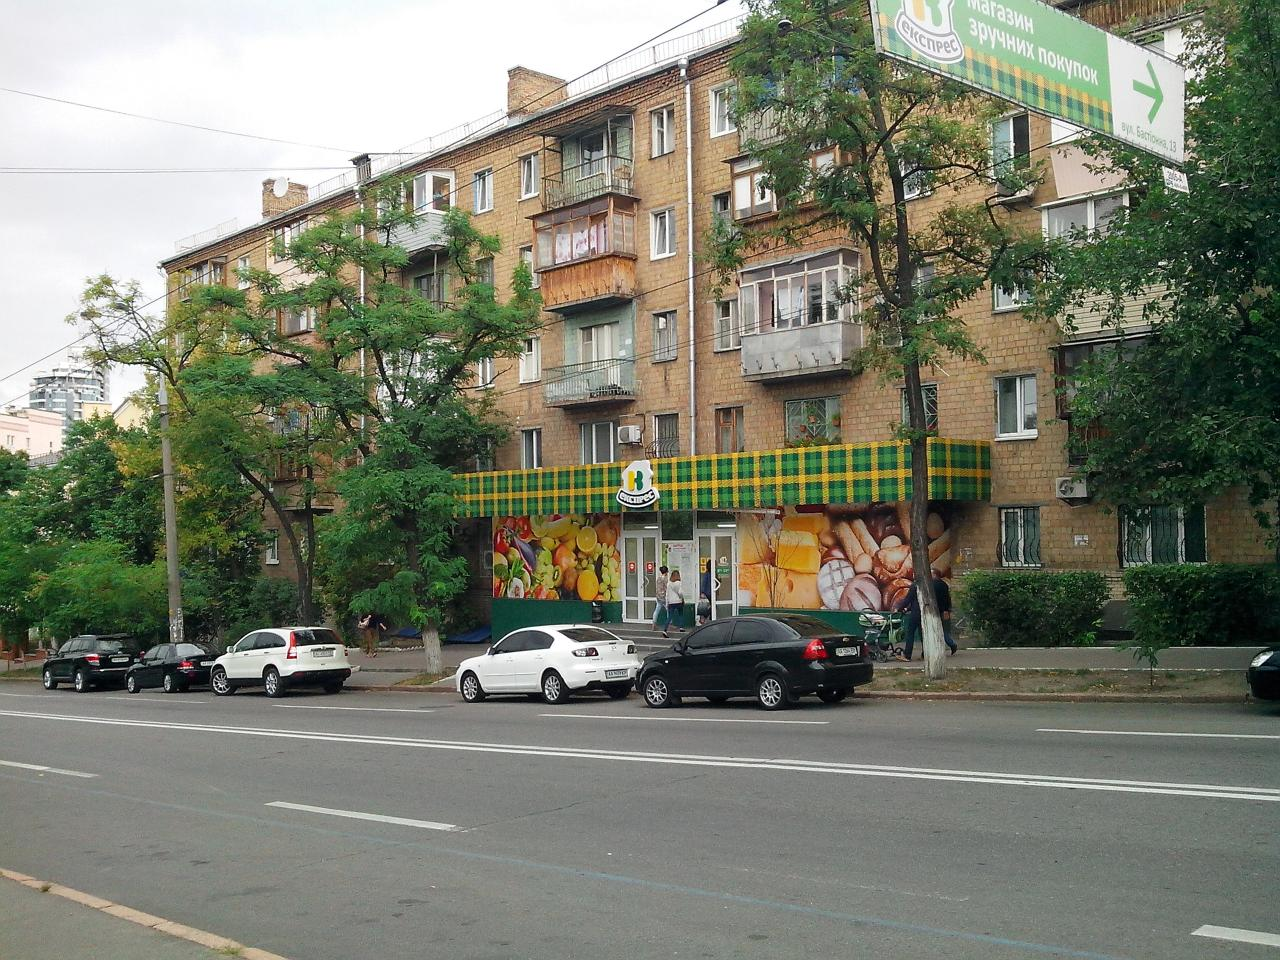
\includegraphics[width=\linewidth]{rpix/IMG_20130826_173208.jpg}

\textit{Арсенальский дом, 2013 год.}
\end{center}

\newpage

\vspace*{\fill}
\begin{center}
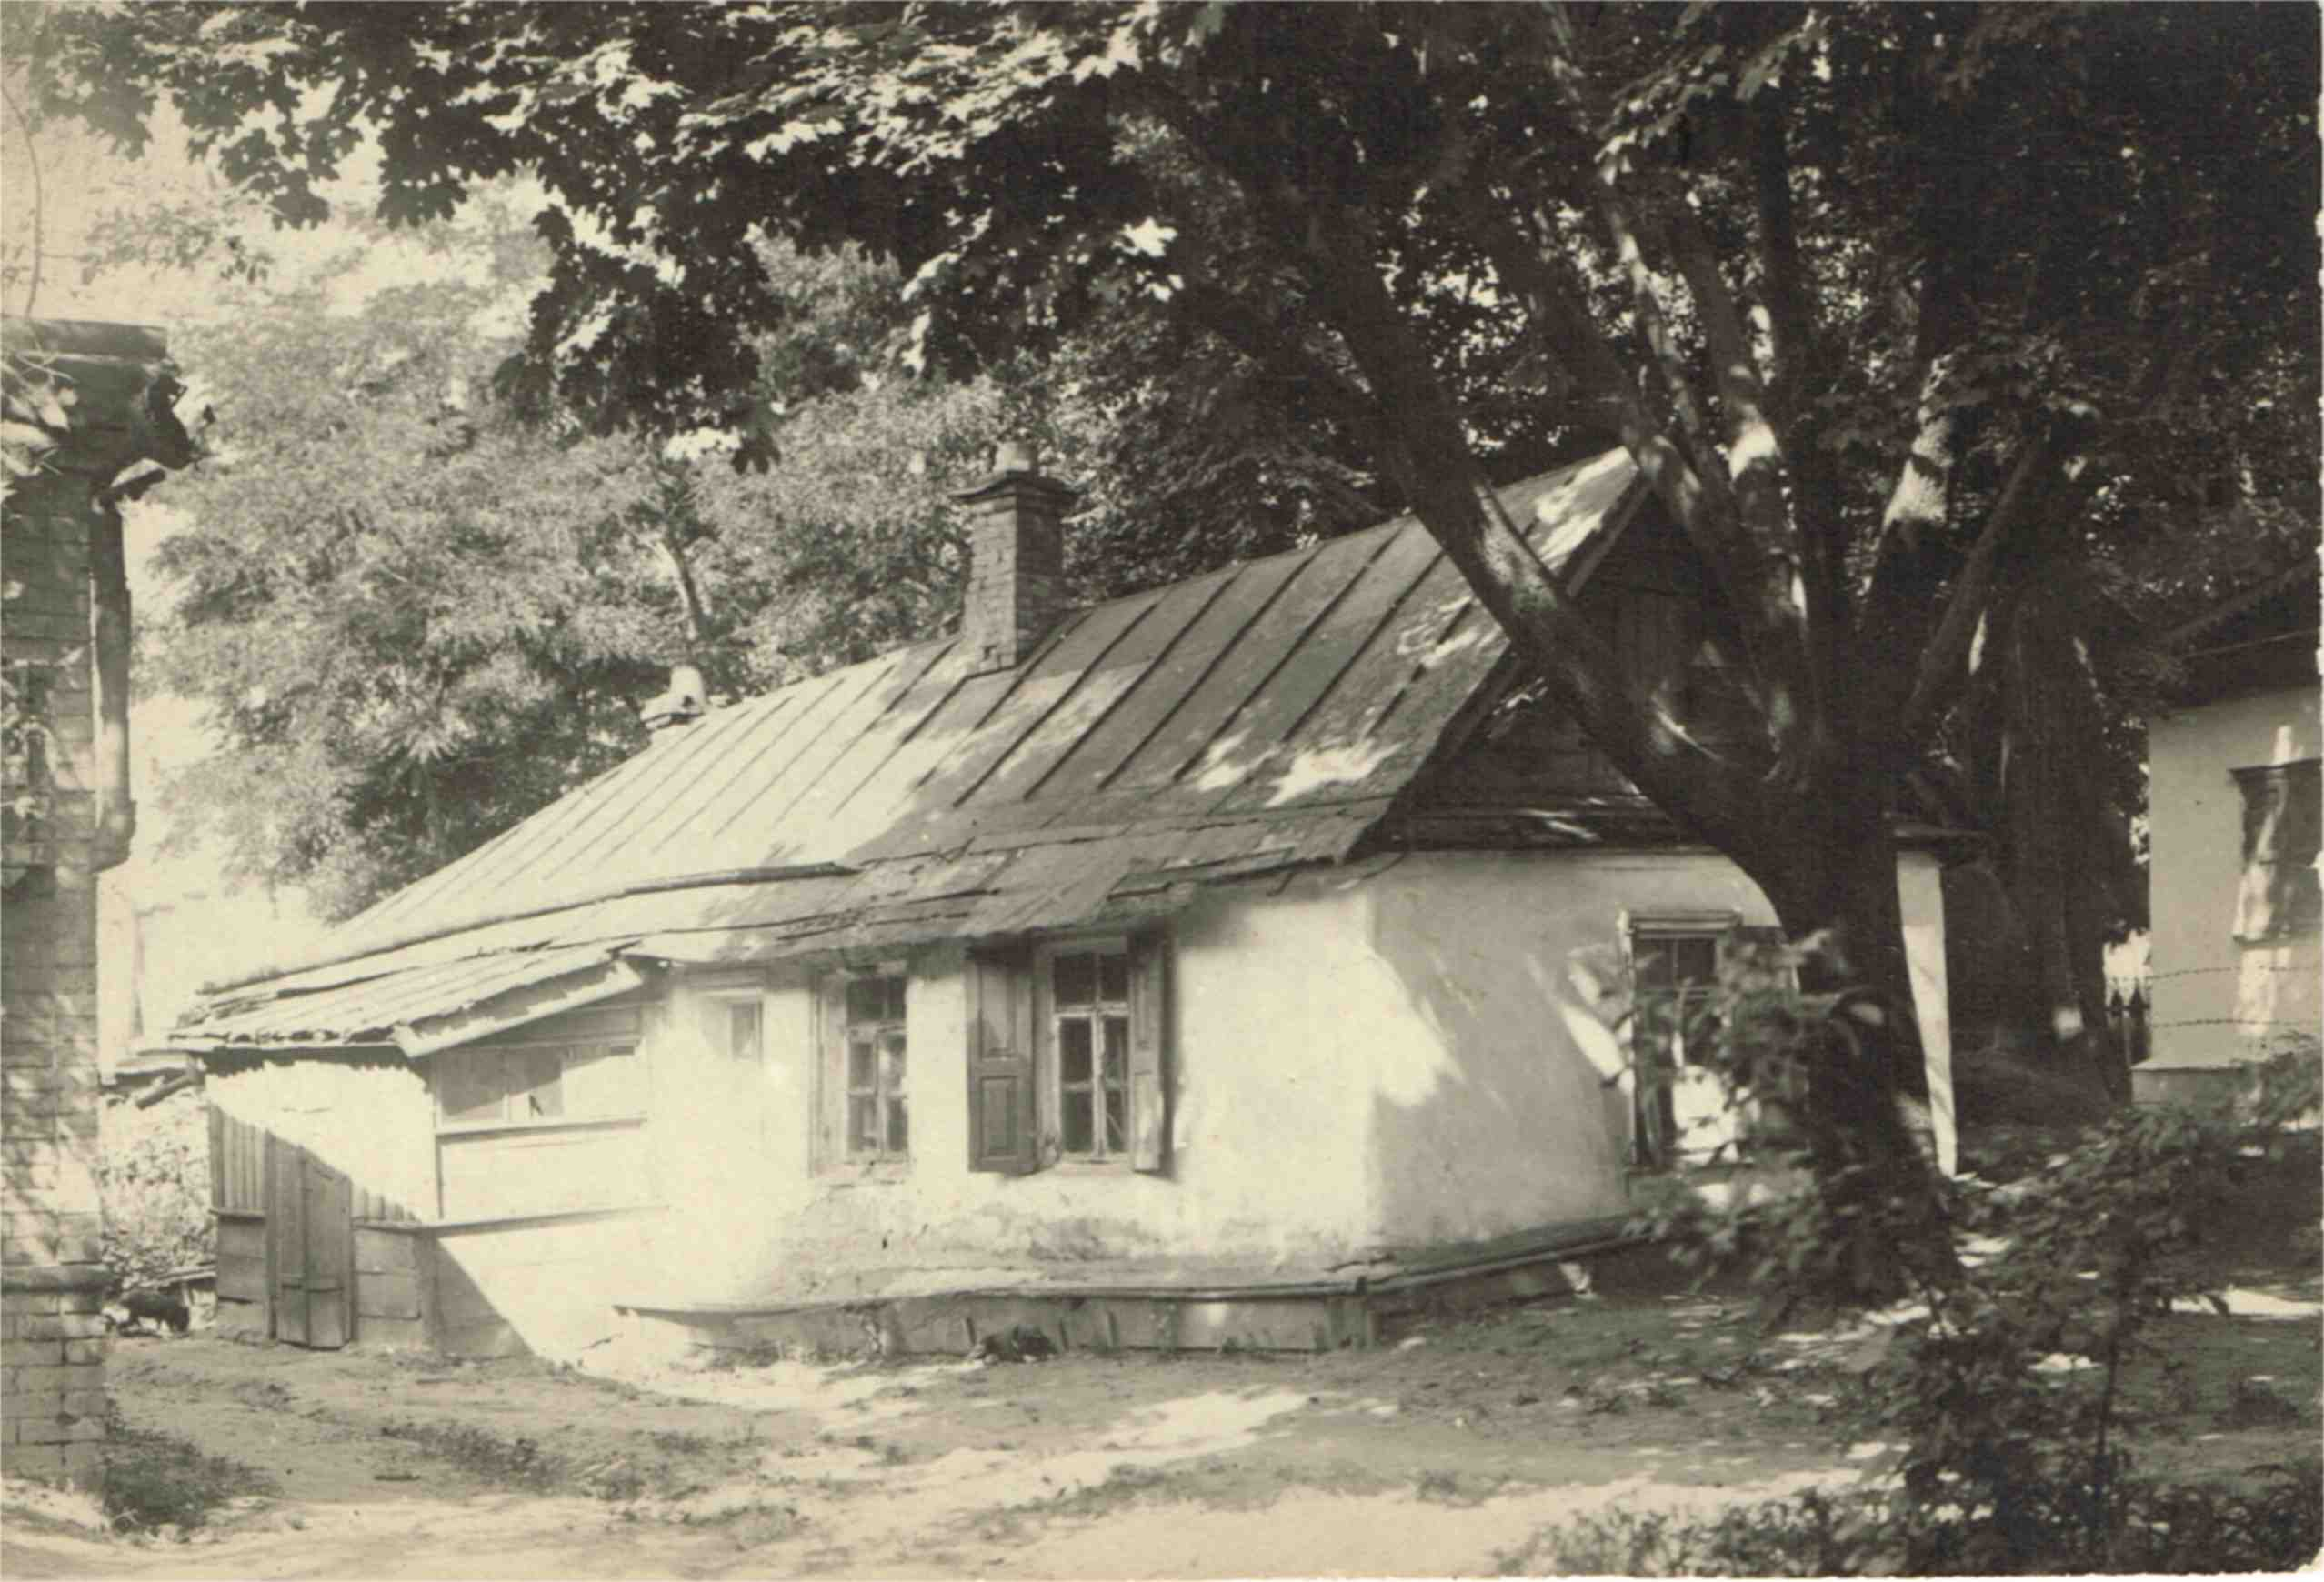
\includegraphics[width=\linewidth]{rpix/bayk.jpg}

\textit{Байкова гора до революции, поселение рядом с кладбищем.}
\end{center}
\vspace*{\fill}
\newpage


\begin{center}
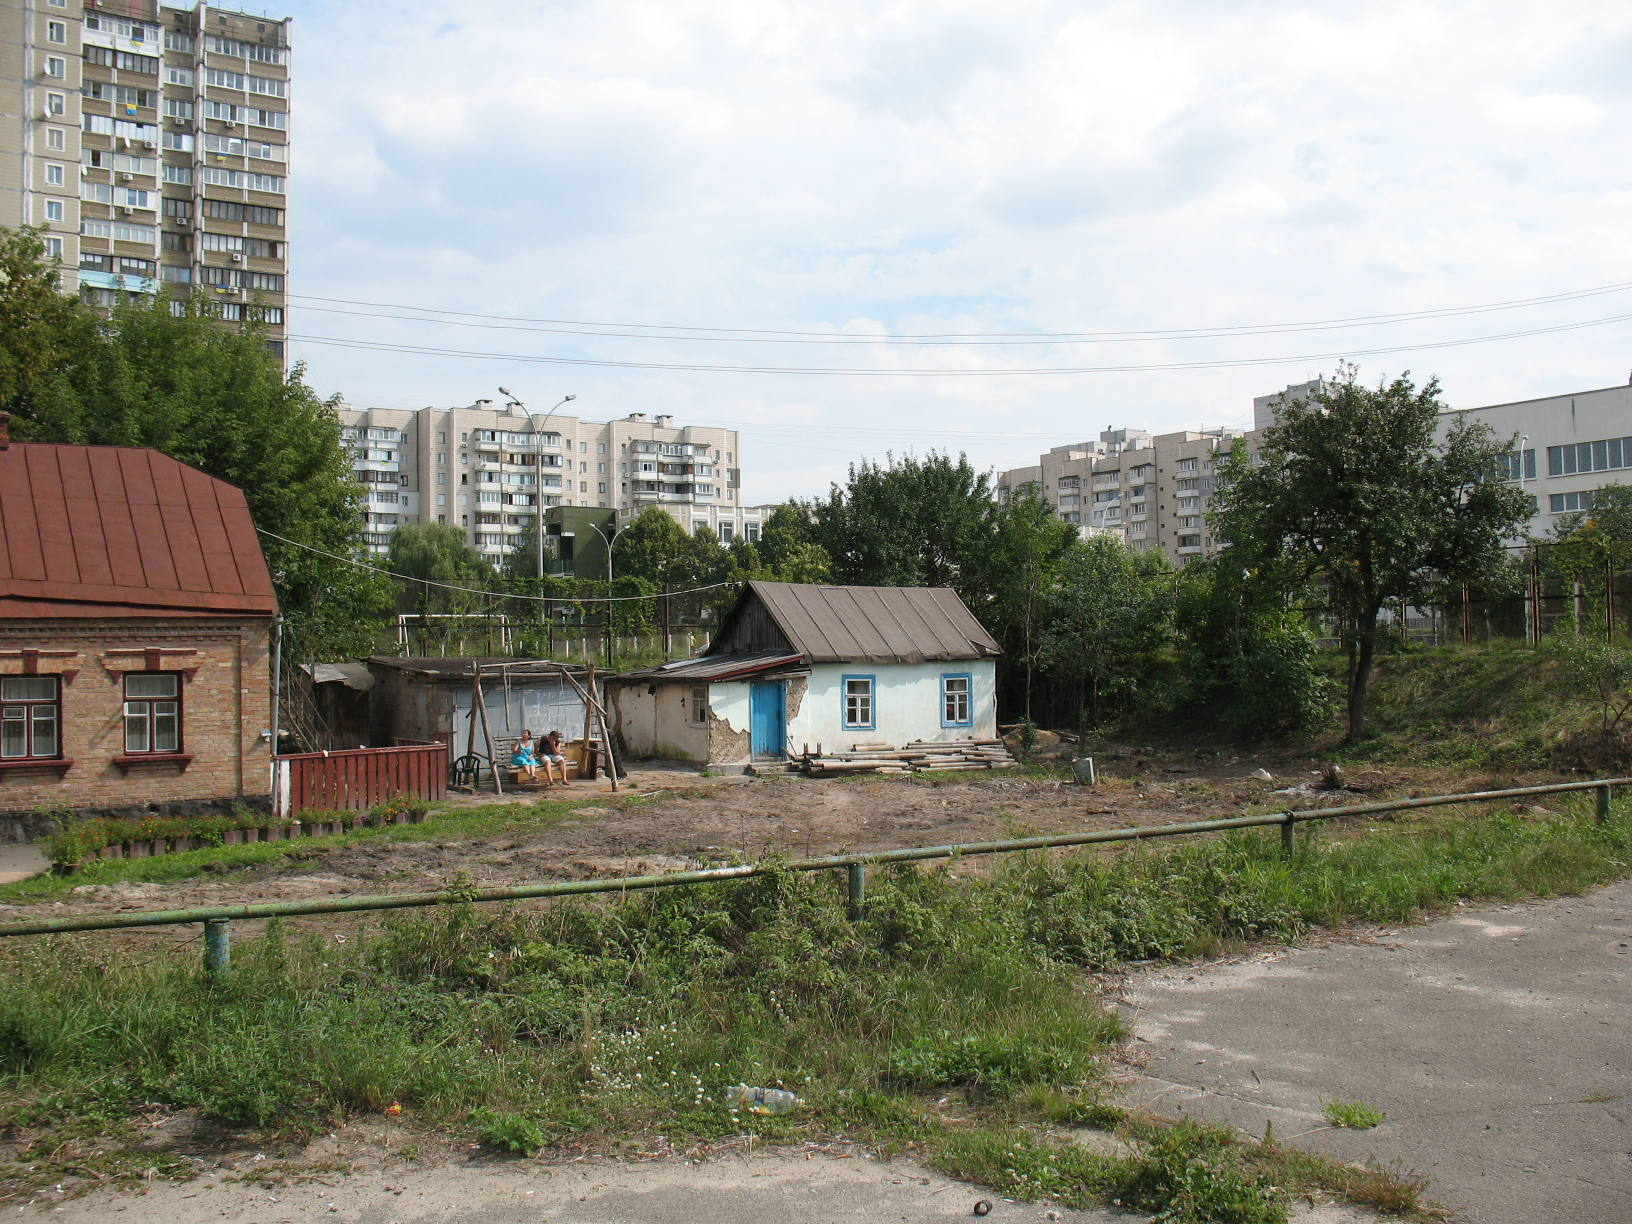
\includegraphics[width=0.95\linewidth]{rpix/IMG_3949.JPG}

\textit{Беличи, остатки юго-западной части села, ныне «13-й микрорайон Беличи».}
\end{center}


\begin{center}
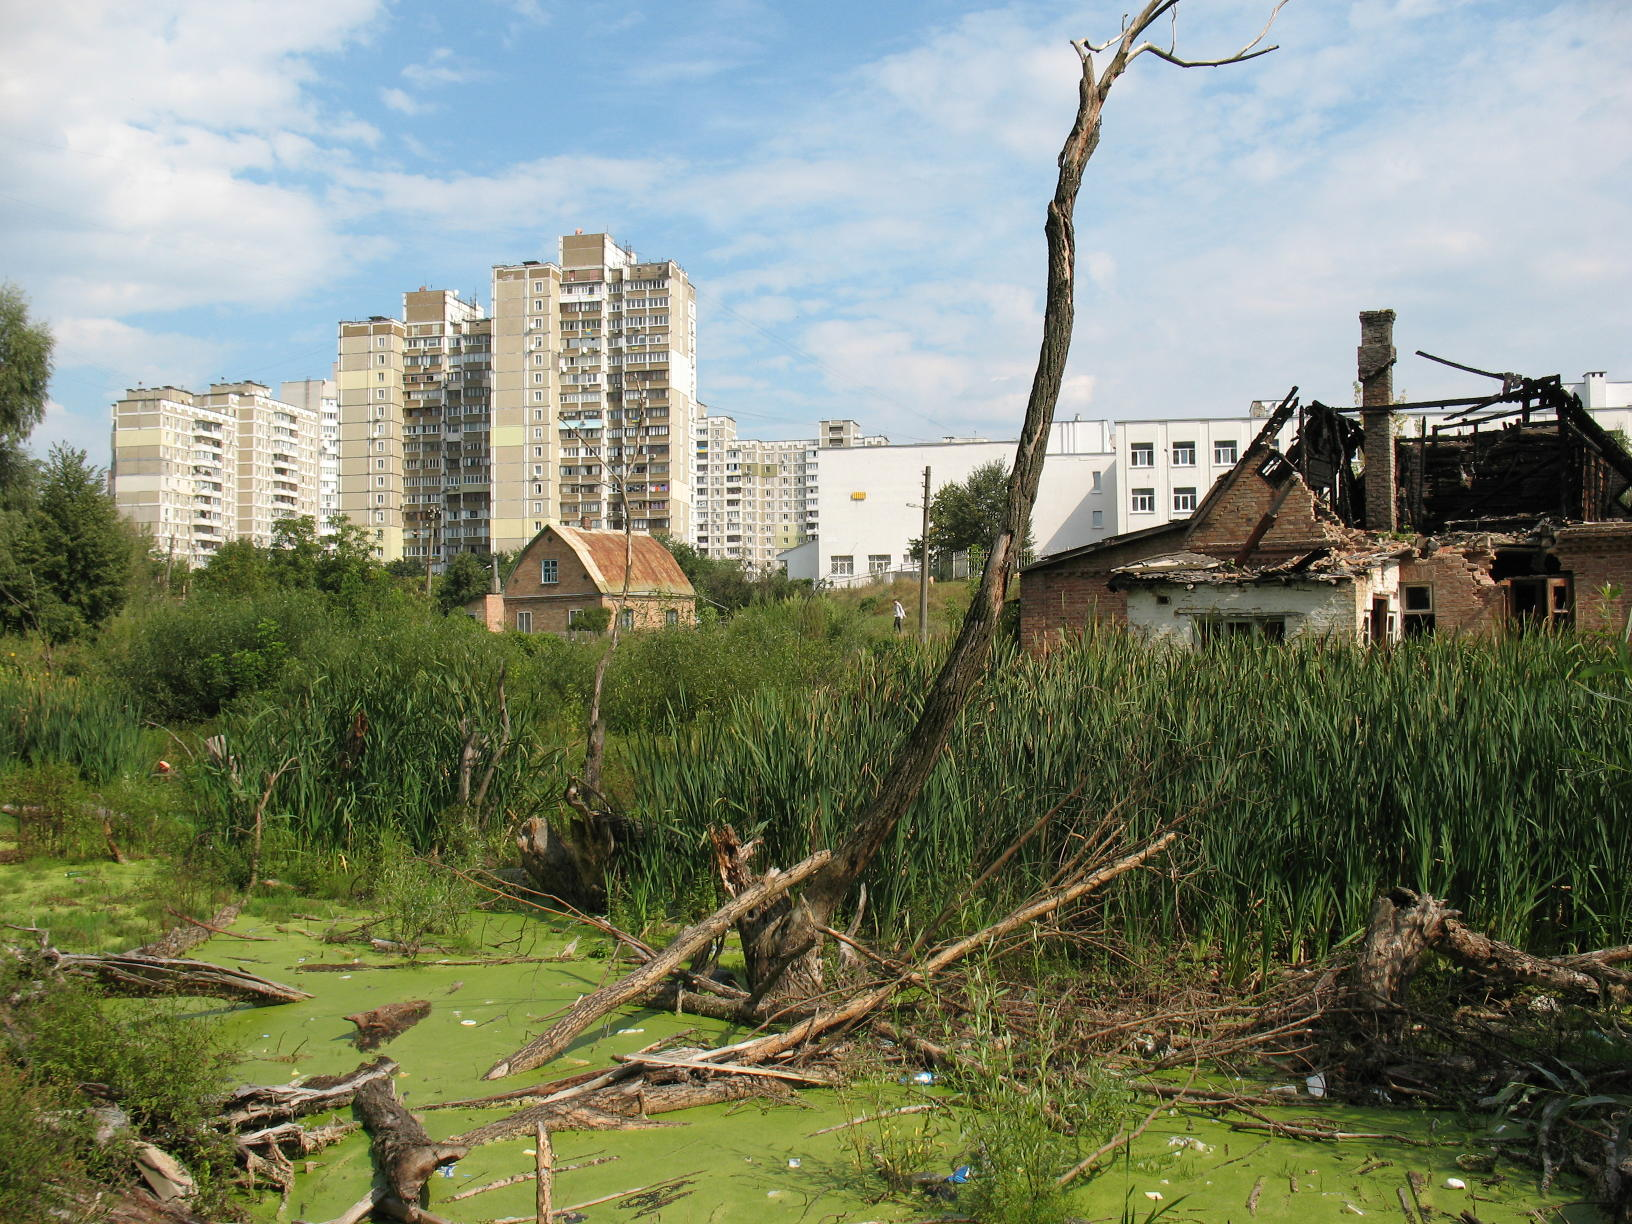
\includegraphics[width=\linewidth]{rpix/IMG_3964.JPG}

\textit{Беличи, почти там же.}
\end{center}


\newpage


\begin{center}
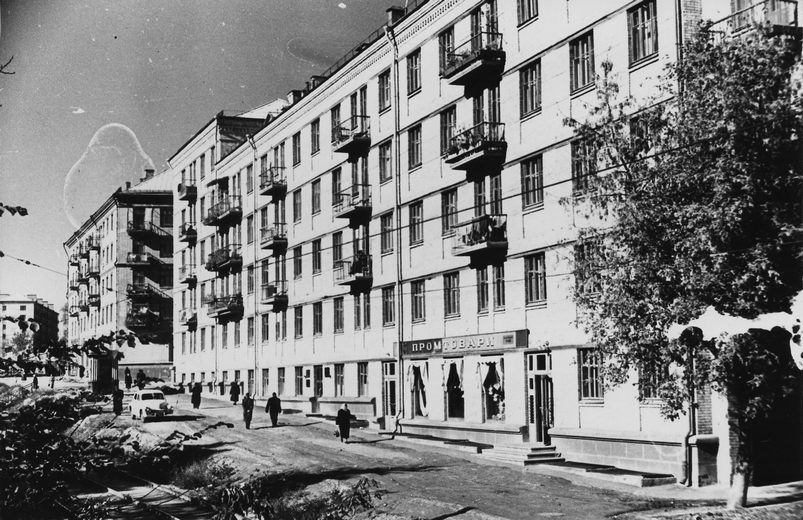
\includegraphics[width=\linewidth]{rpix/belor-14.jpg}

\textit{Расположенная в овраге Белорусская улица, слева видны трамвайные рельсы. Там по дну оврага раньше протекал ручей Скоморох, ныне заточенный в коллектор.}
\end{center}


\begin{center}
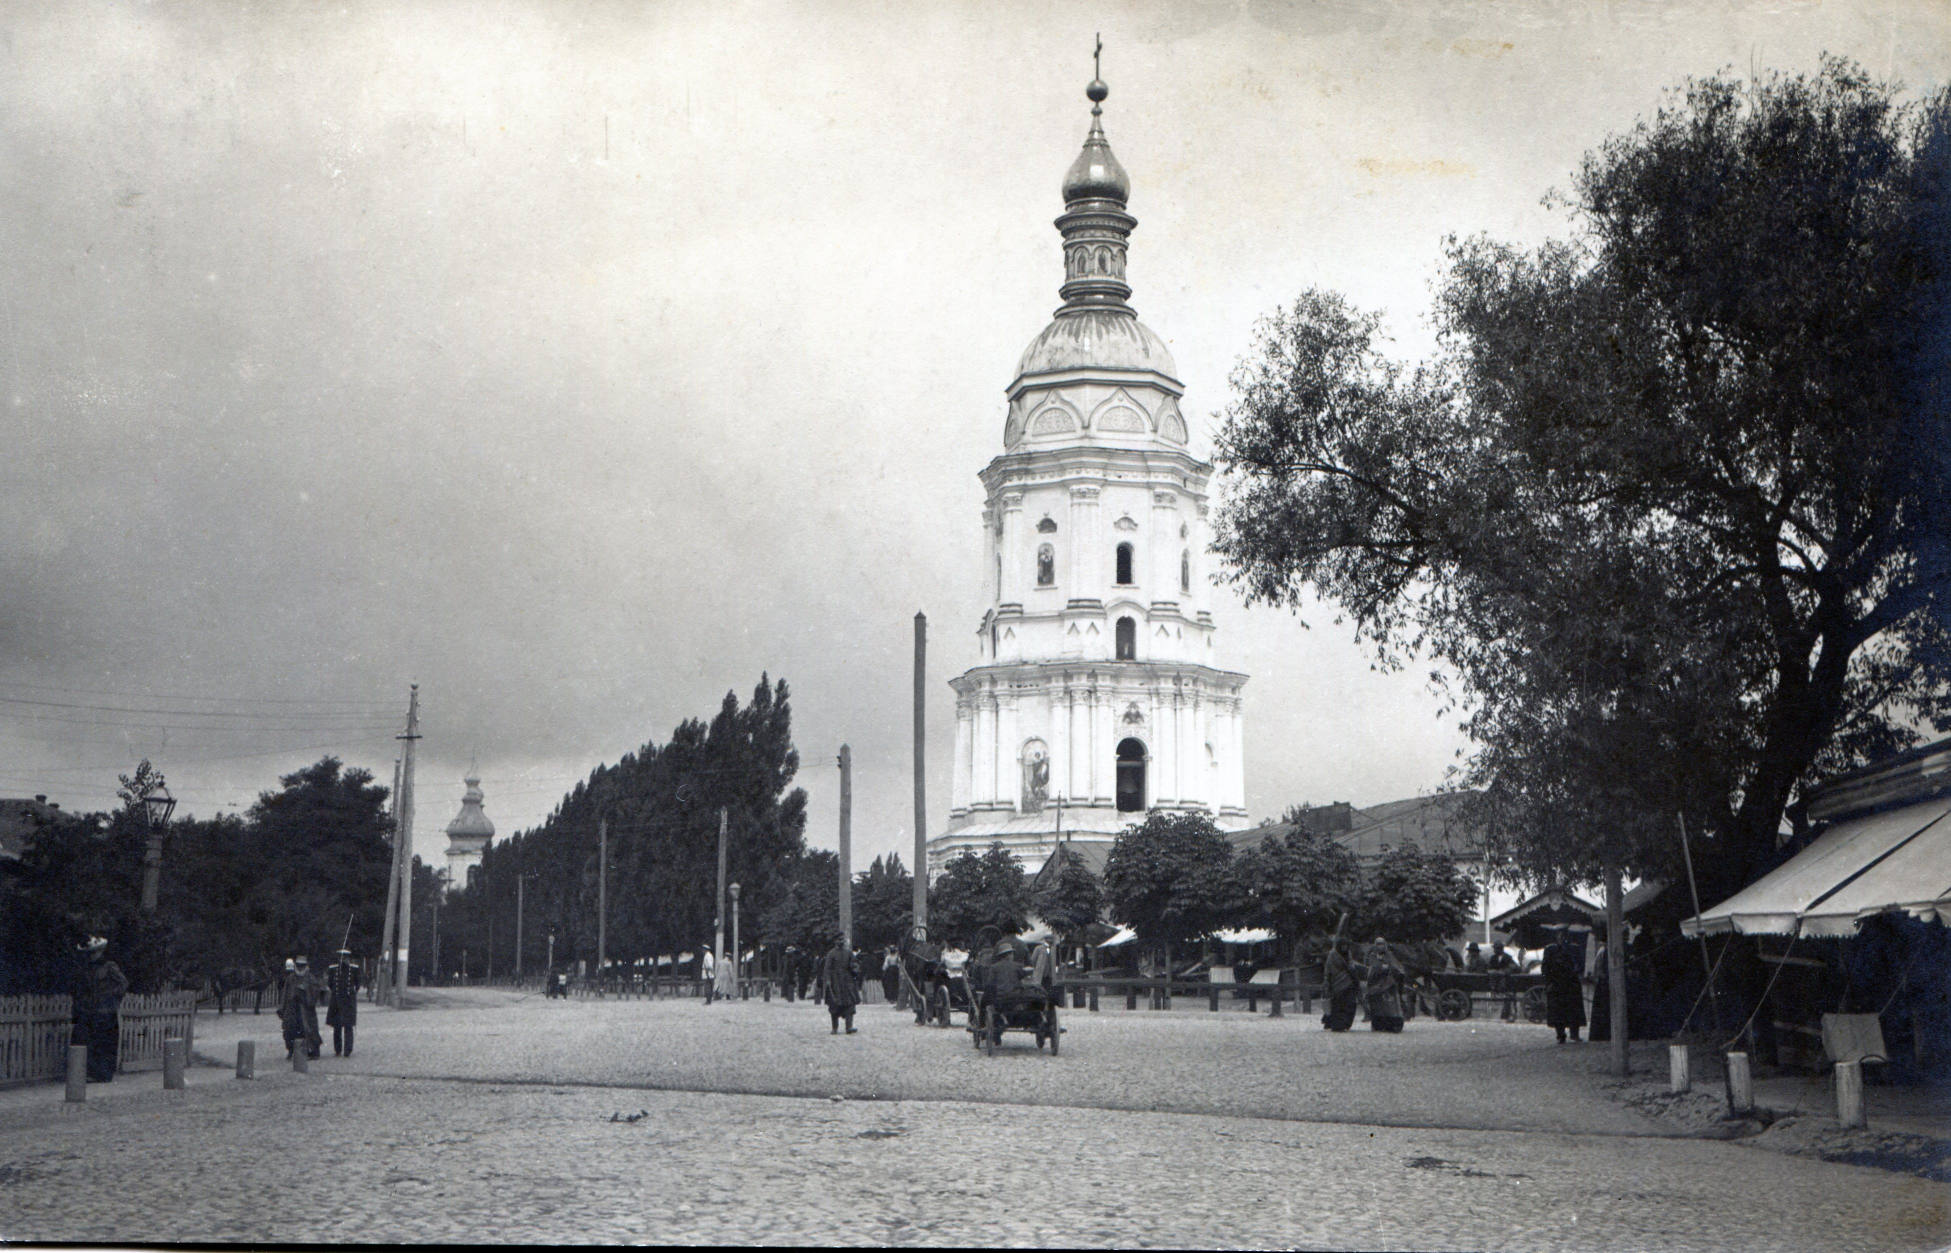
\includegraphics[width=\linewidth]{rpix/bolnikolay.jpg}

\textit{Большой Николай, колокольня.}
\end{center}



\begin{center}
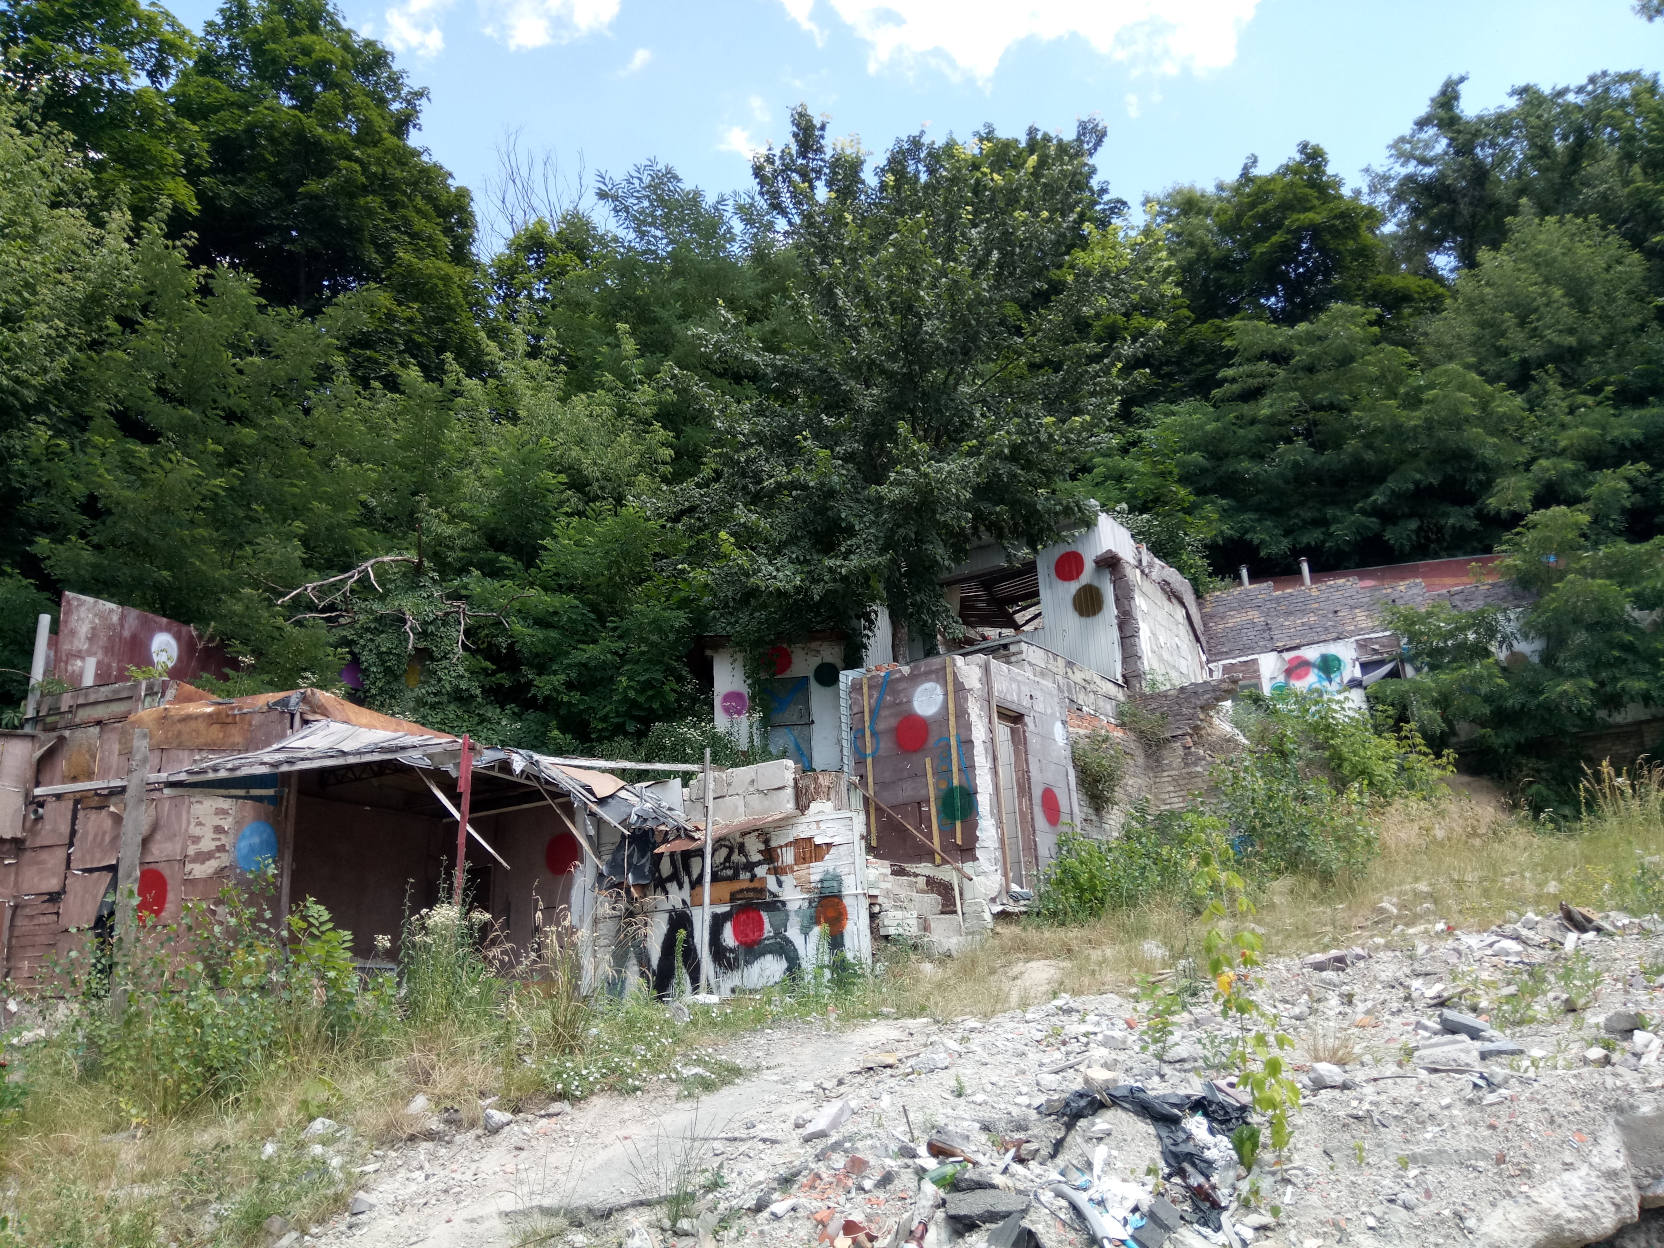
\includegraphics[width=\linewidth]{rpix/IMG_20190619_125950.jpg}

\textit{Окрестности источника Бусловки.}
\end{center}


\begin{center}
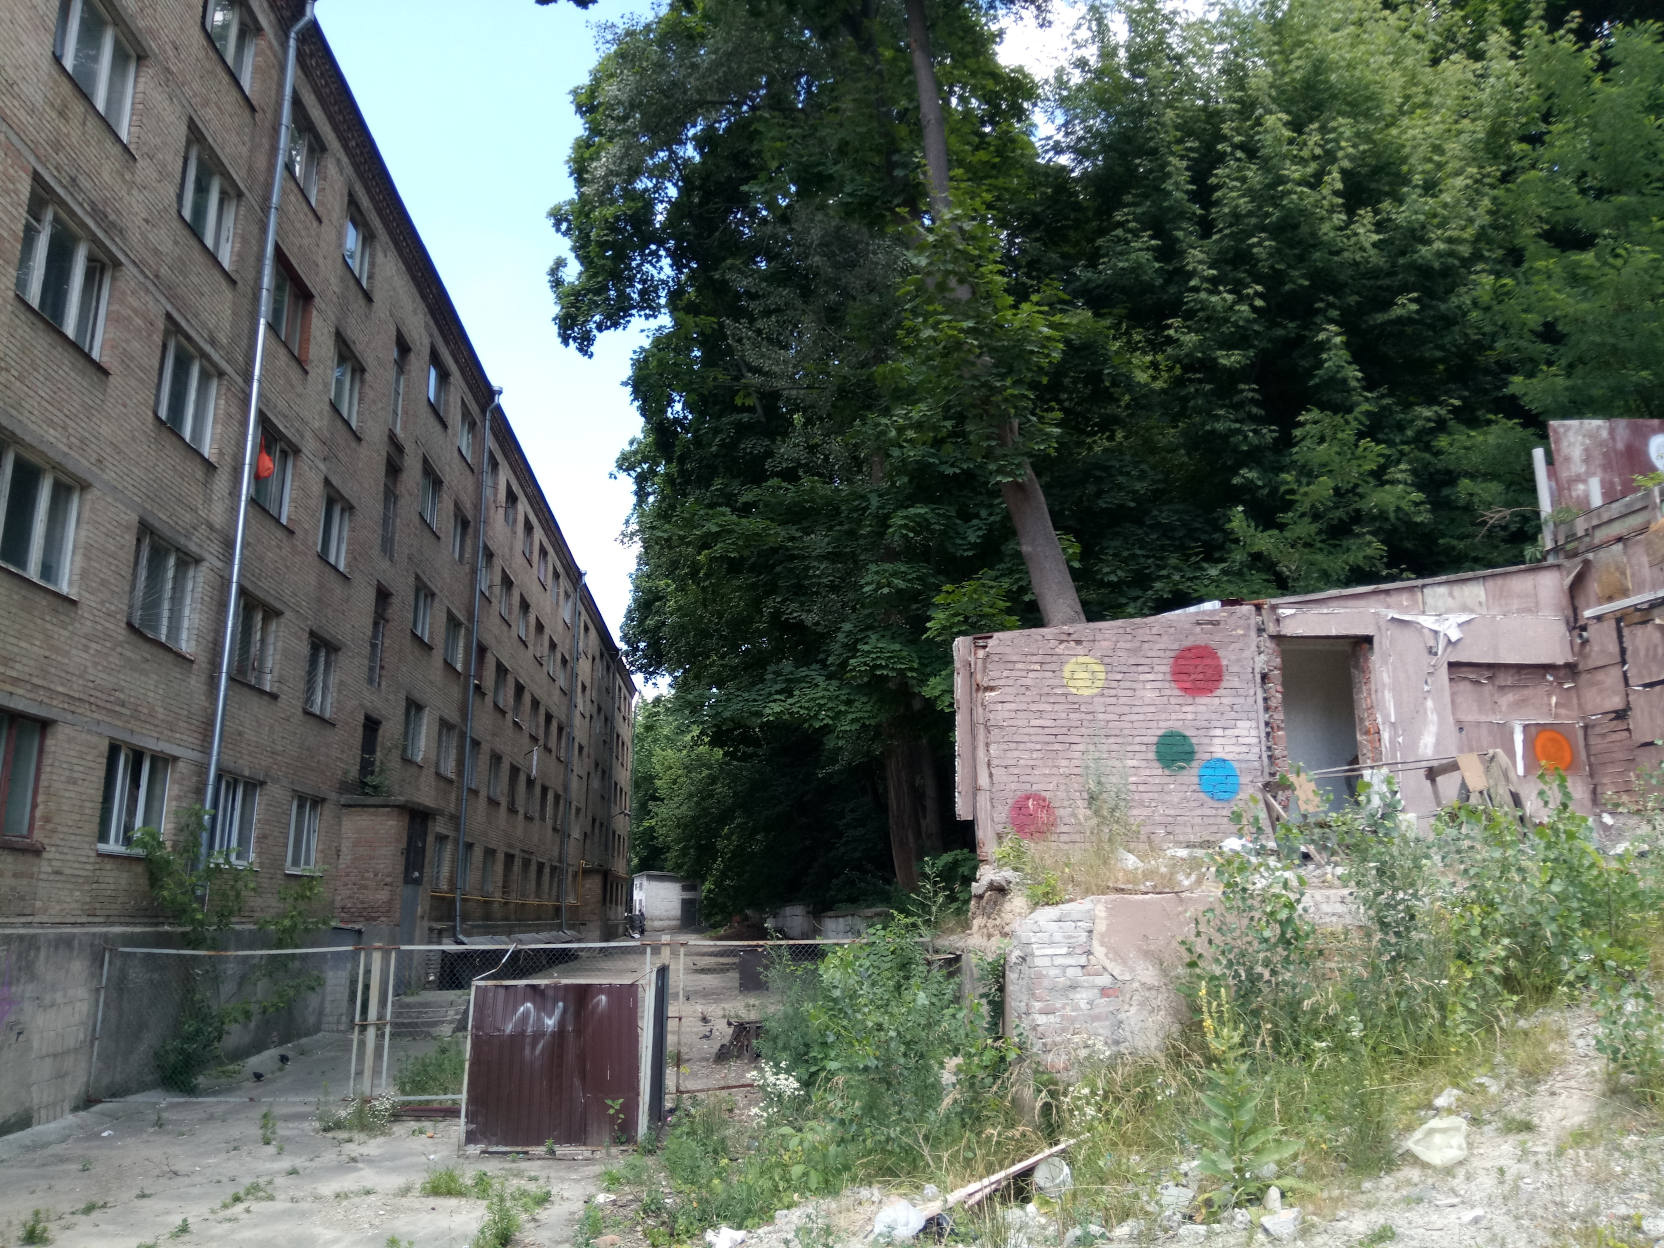
\includegraphics[width=\linewidth]{rpix/IMG_20190619_125951.jpg}

\textit{Окрестности источника Бусловки.}
\end{center}


\newpage


\begin{center}
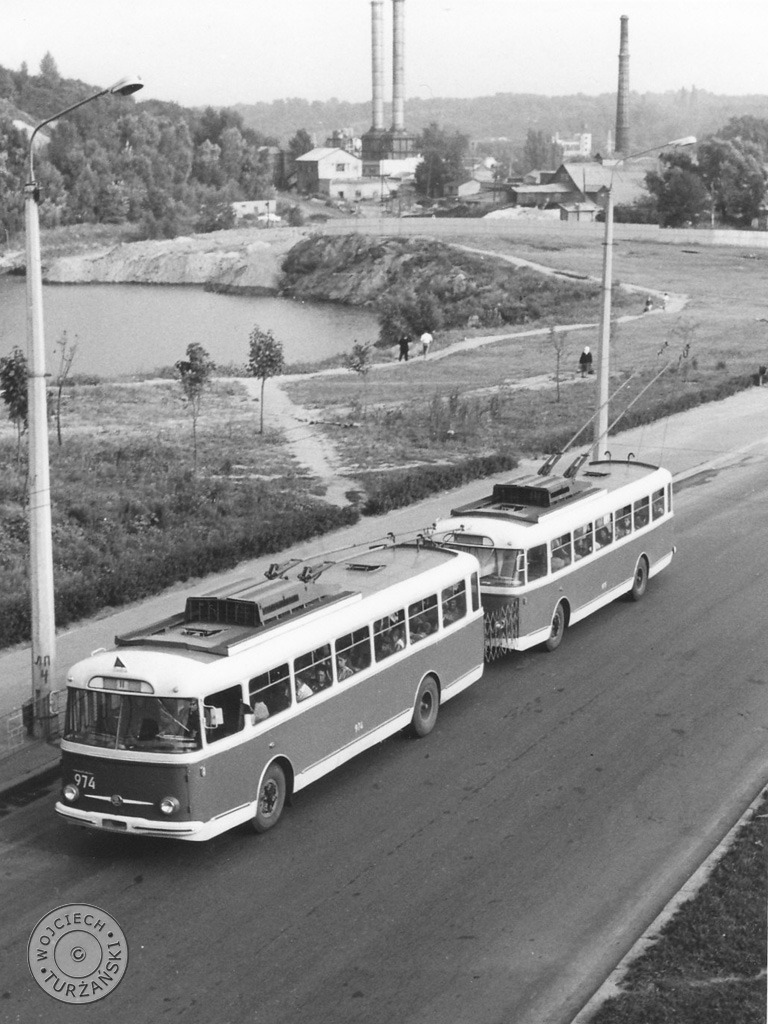
\includegraphics[width=\linewidth]{rpix/1973.jpg}

\textit{Глинка, озеро в 1971 году. Снимок Войтеха Туржанского. Слева – Черная гора, на заднем плане, за кирпичным заводом, на другой горе (за Лыбедью) – Саперная слободка.}
\end{center}

\newpage


\begin{center}
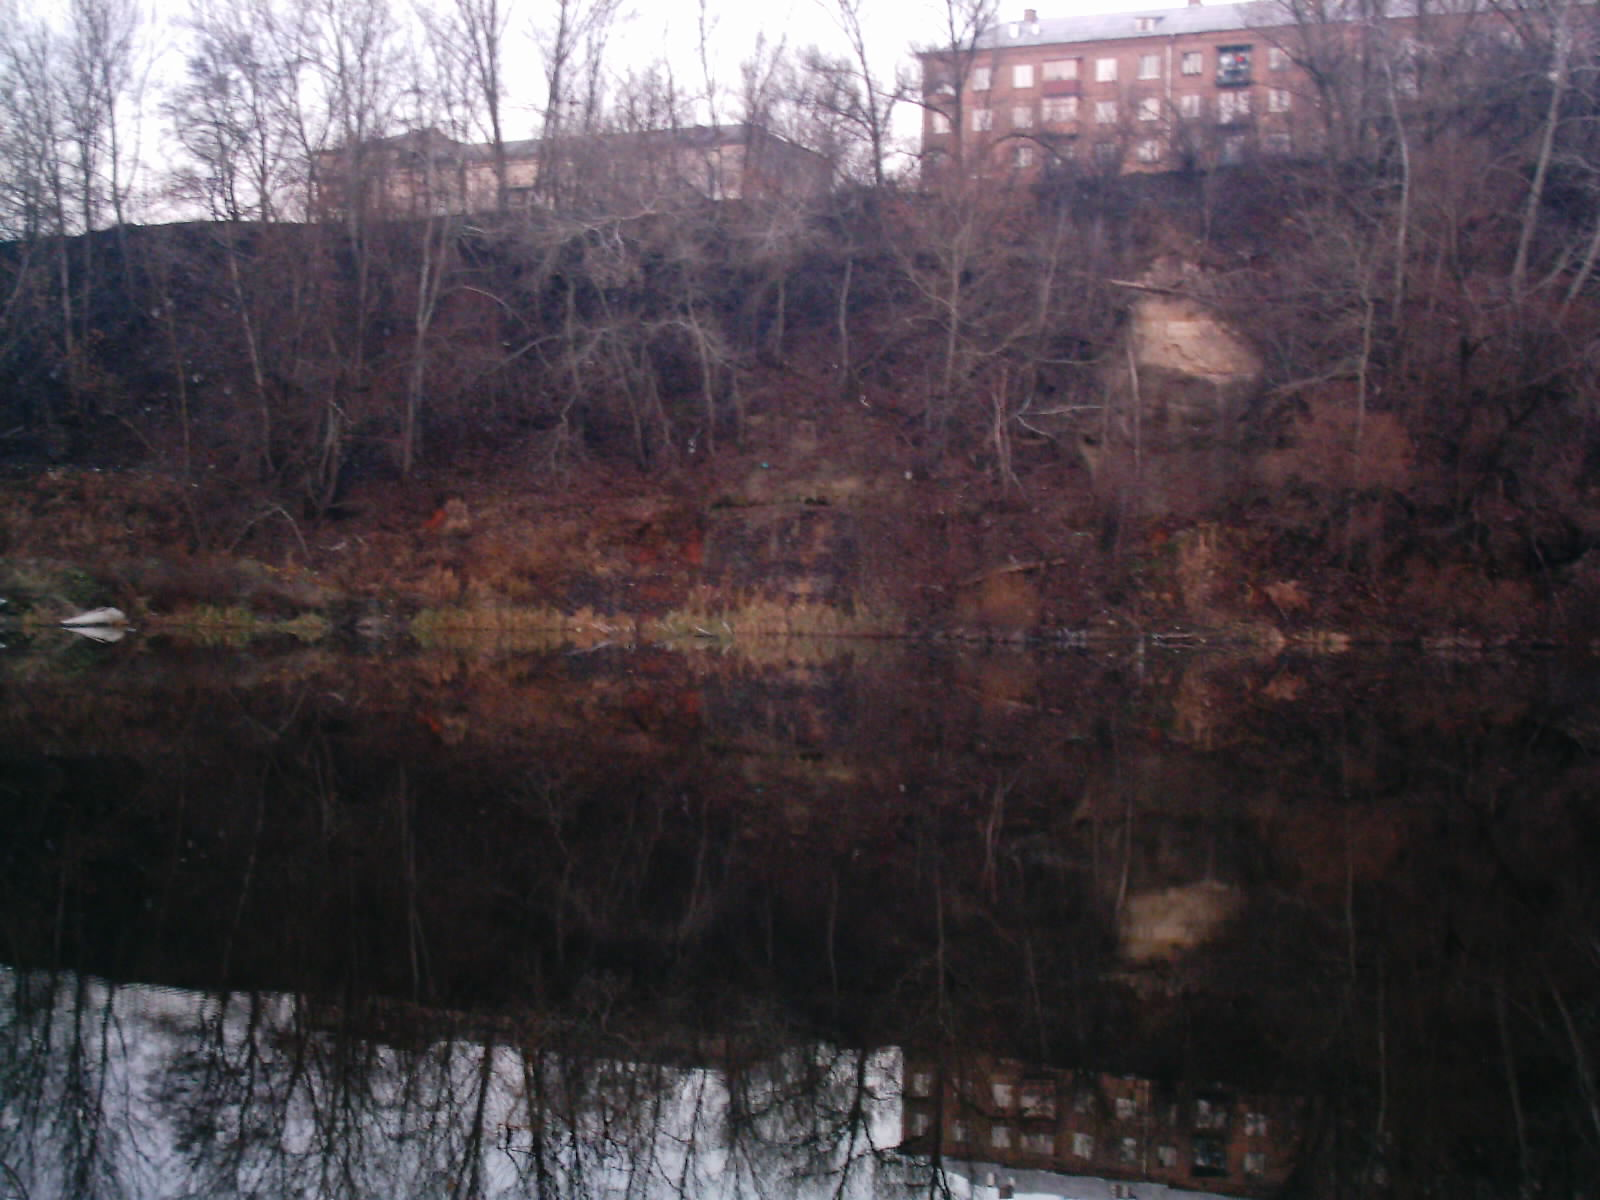
\includegraphics[width=\linewidth]{rpix/imag0025.jpg}

\textit{Глинка, 2005 год. Вид на хрущовки над озером.}
\end{center}



\begin{center}
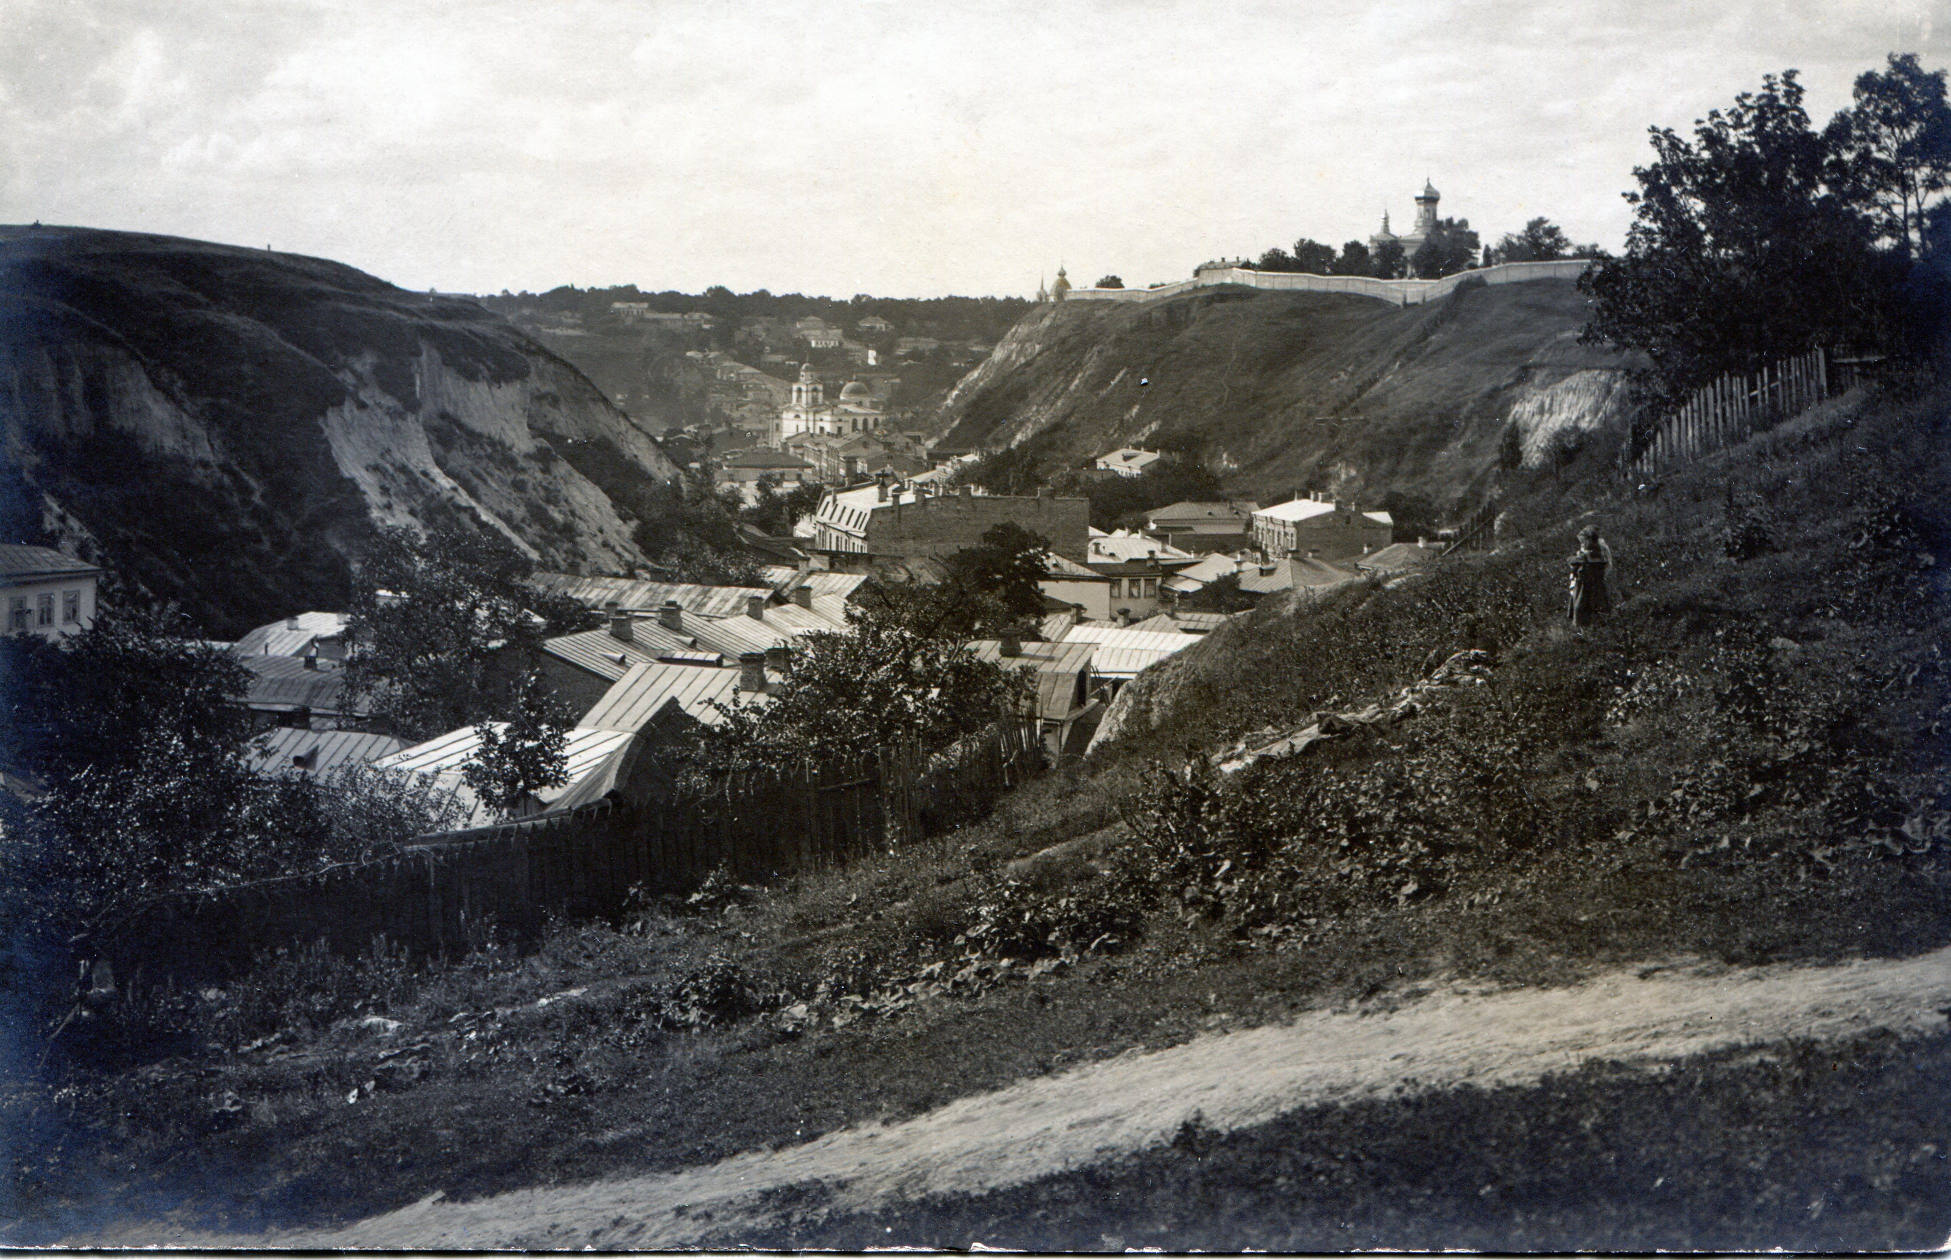
\includegraphics[width=\linewidth]{rpix/gonch.jpg}

\textit{Гончары, вид на Гончаровскую улицу. Конечно же, дореволюционная открытка.}
\end{center}


\newpage


\begin{center}
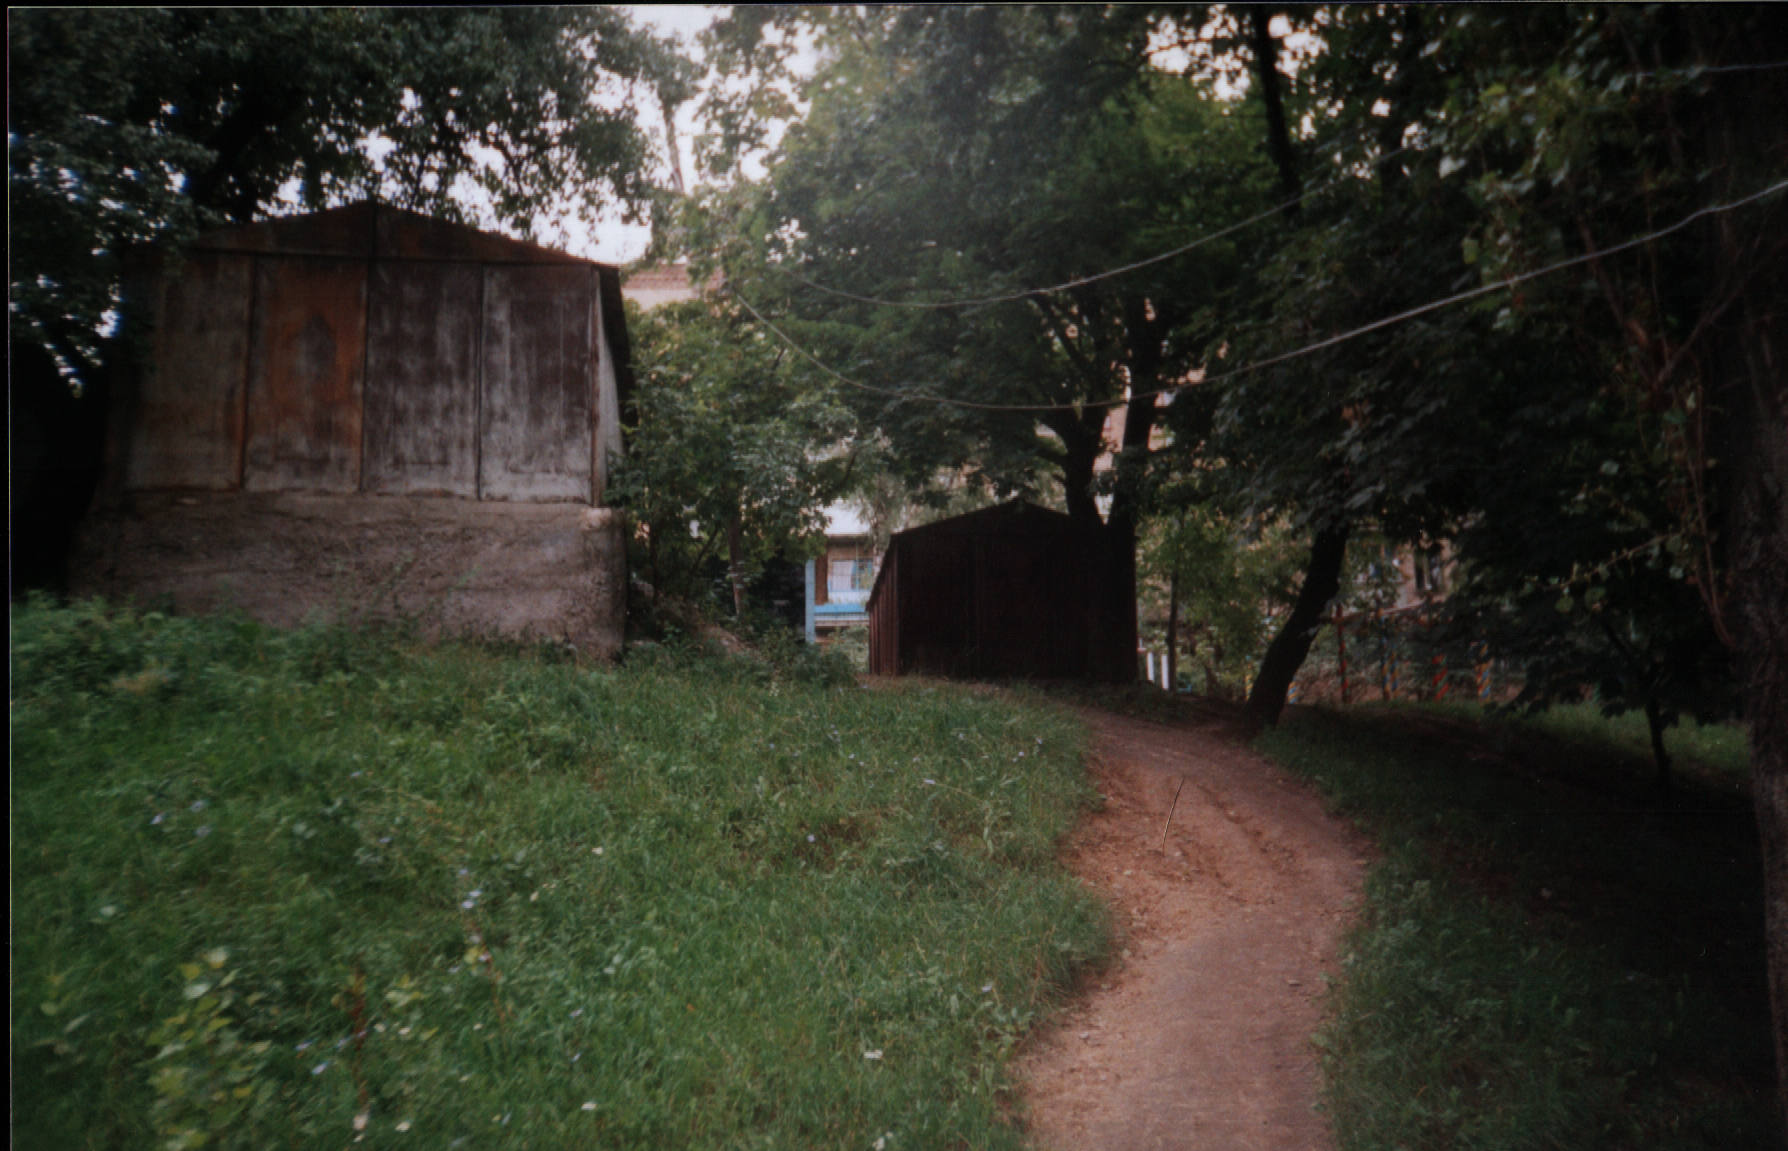
\includegraphics[width=\linewidth]{rpix/gorka.jpg}

\textit{Горка, 2003 год.}
\end{center}

\begin{center}
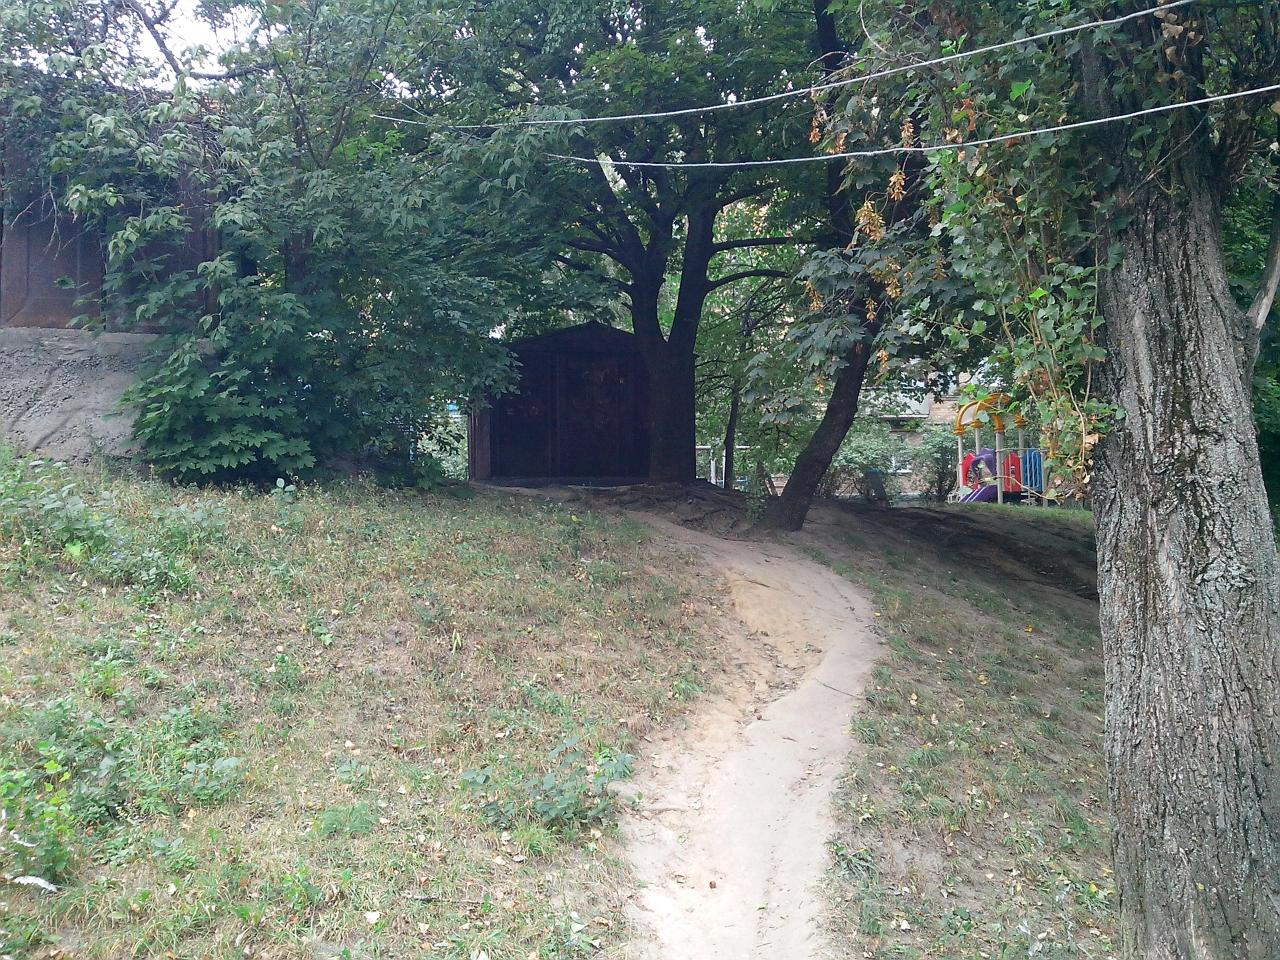
\includegraphics[width=\linewidth]{rpix/IMG_20130826_143424.jpg}

\textit{Горка, 2013 год.}
\end{center}


\newpage
\vspace*{\fill}
\begin{center}
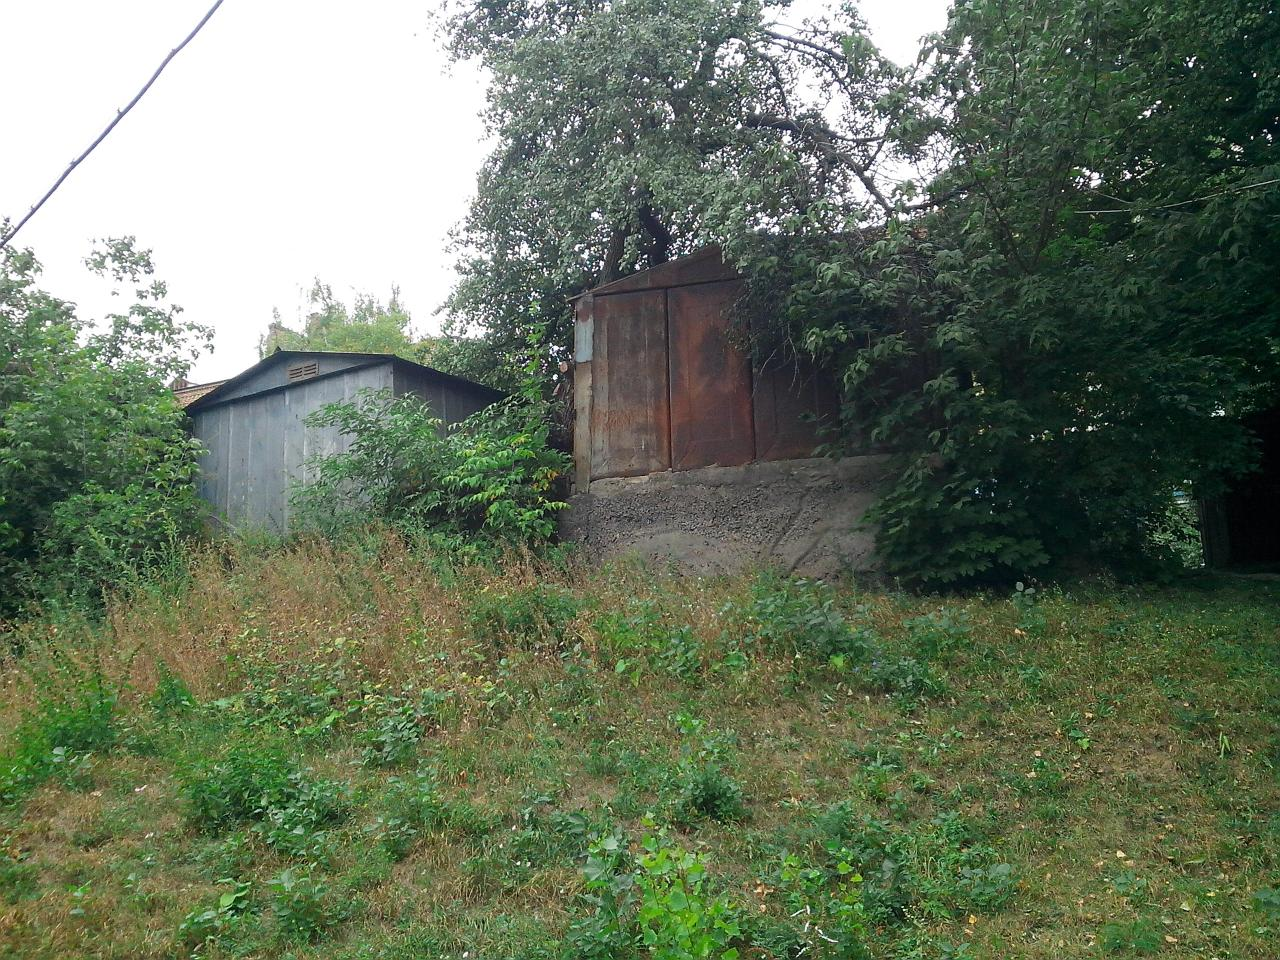
\includegraphics[width=\linewidth]{rpix/IMG_20130826_143421.jpg}

\textit{Горка, 2013 год, вид чуть левее. За серым гаражом – осколок частного сектора в несколько домов, с узеньким переулком между дворами.}
\end{center}
\vspace*{\fill}

\newpage
\vspace*{\fill}

\begin{center}
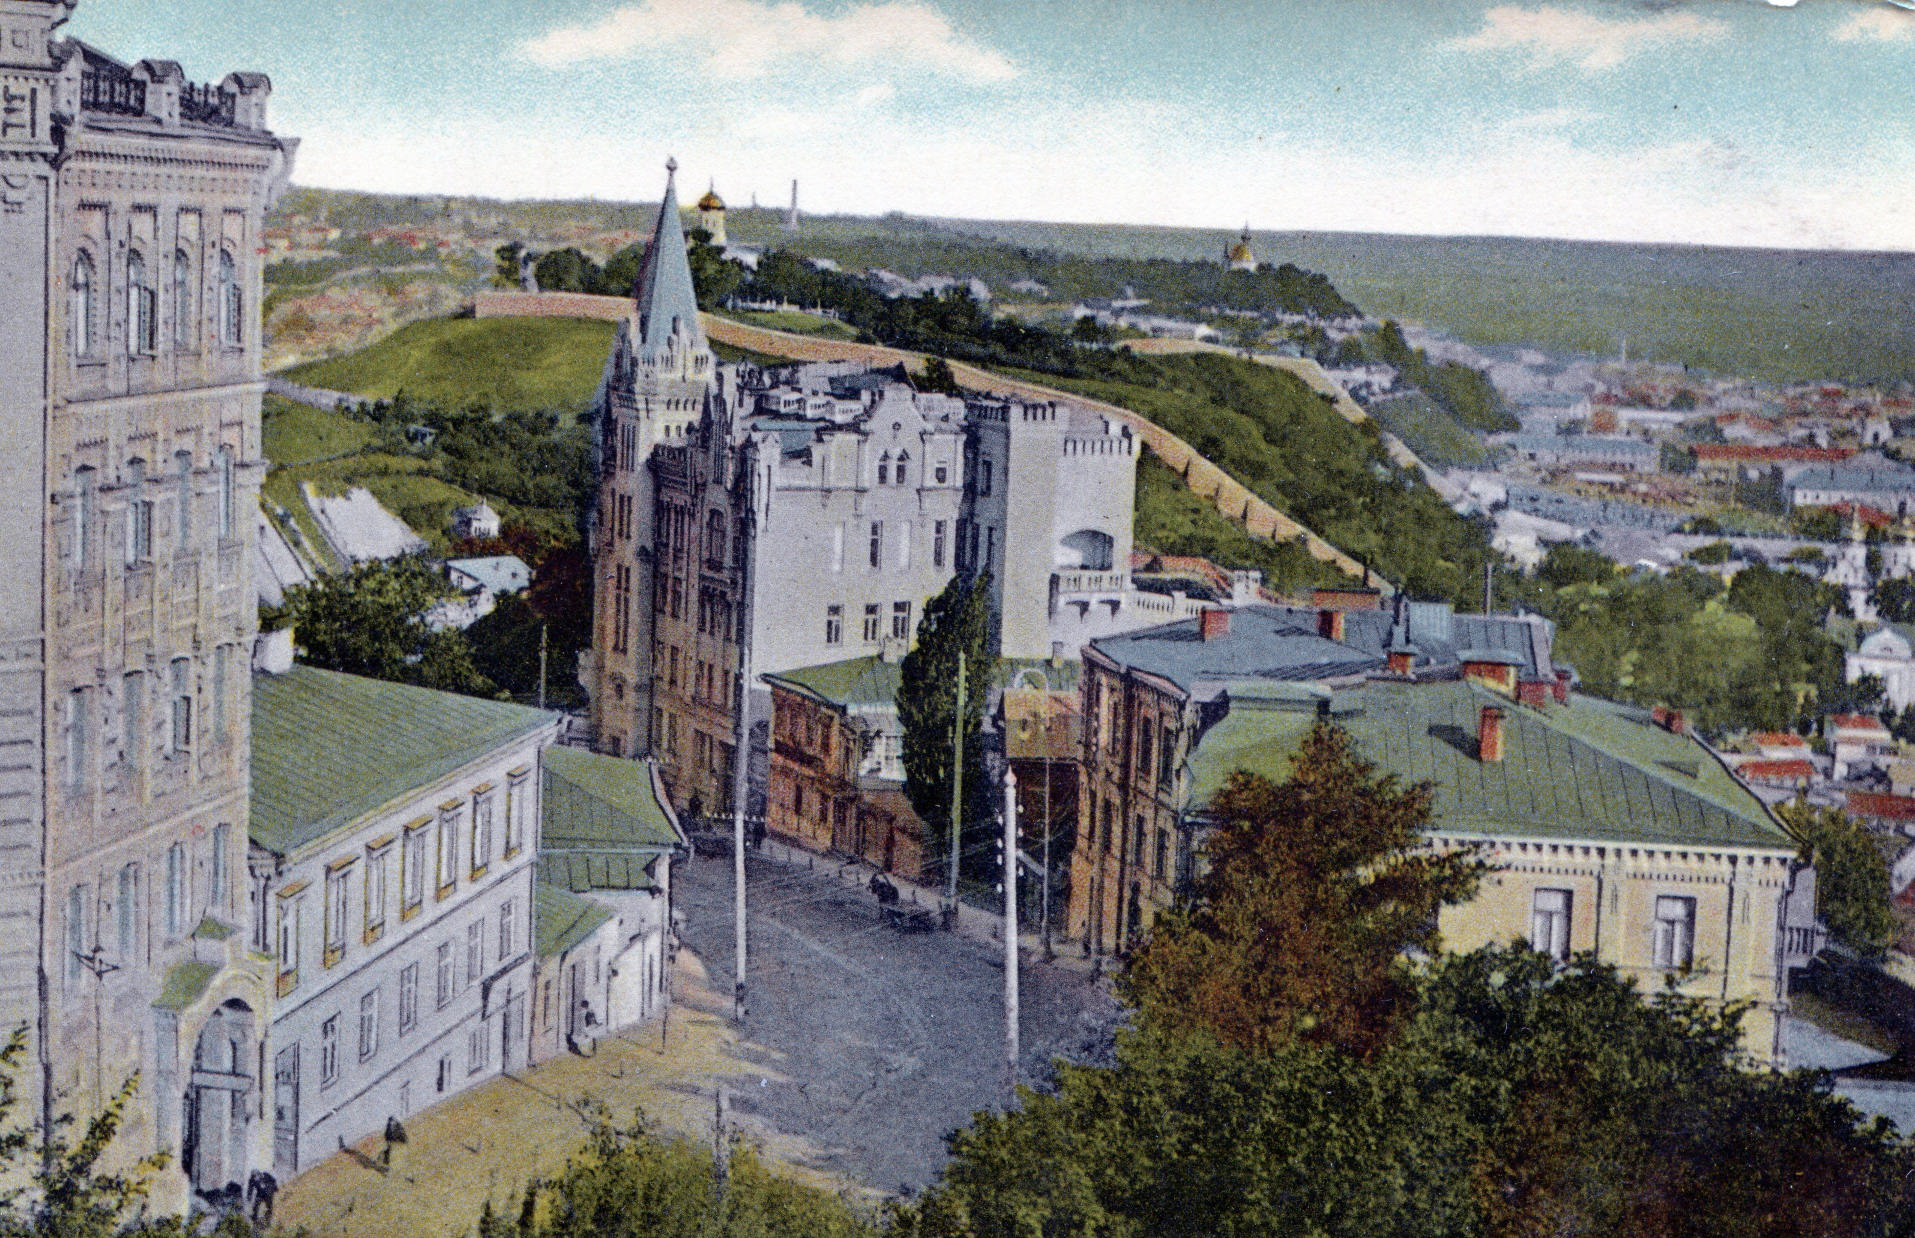
\includegraphics[width=\linewidth]{rpix/domrich.jpg}

\textit{Дом Ричарда, дореволюционная открытка. За ним видно гору Киселевку с кирпичной кладбищенской стеной – там было кладбище Флоровского монастыря, разоренные остатки коего, равно как и стену, можно посетить и в наши дни.}
\end{center}
\vspace*{\fill}


\newpage

\begin{center}
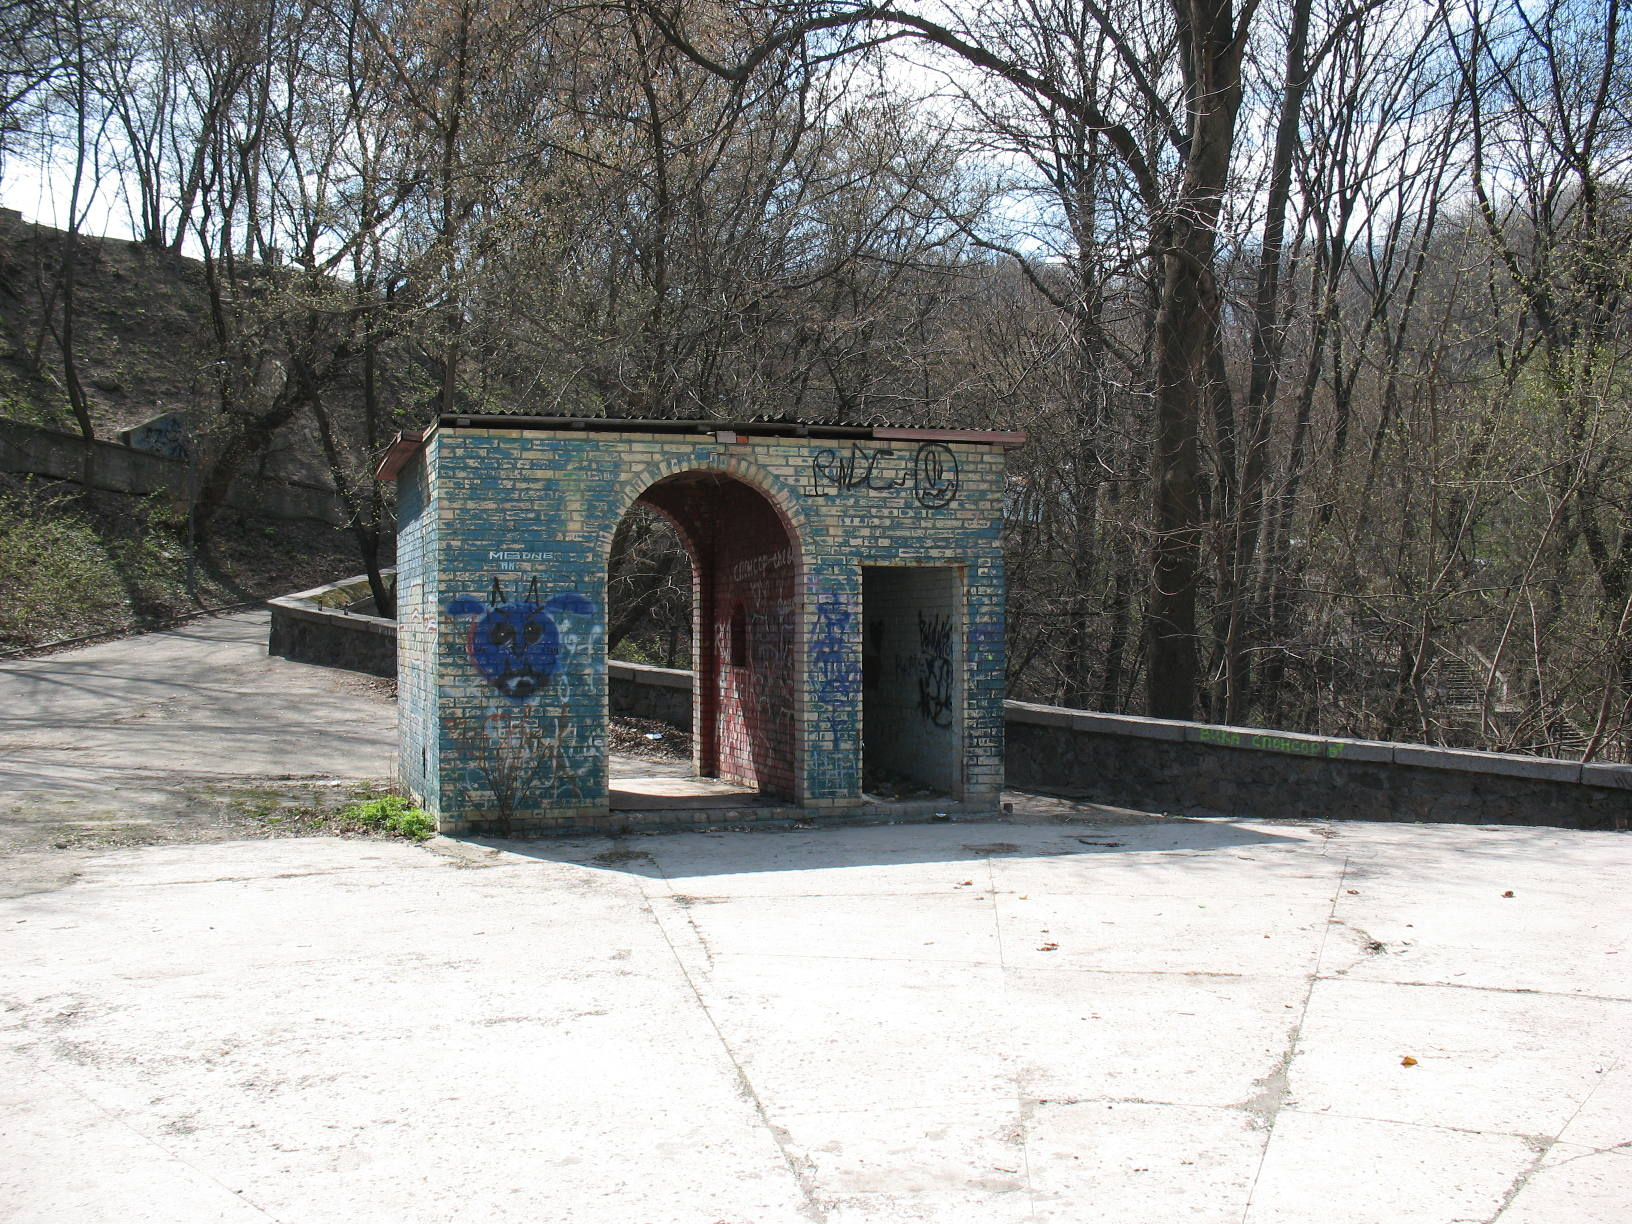
\includegraphics[width=\linewidth]{rpix/IMG_1401.JPG}

\textit{Жаба. Вход.}
\end{center}


\begin{center}
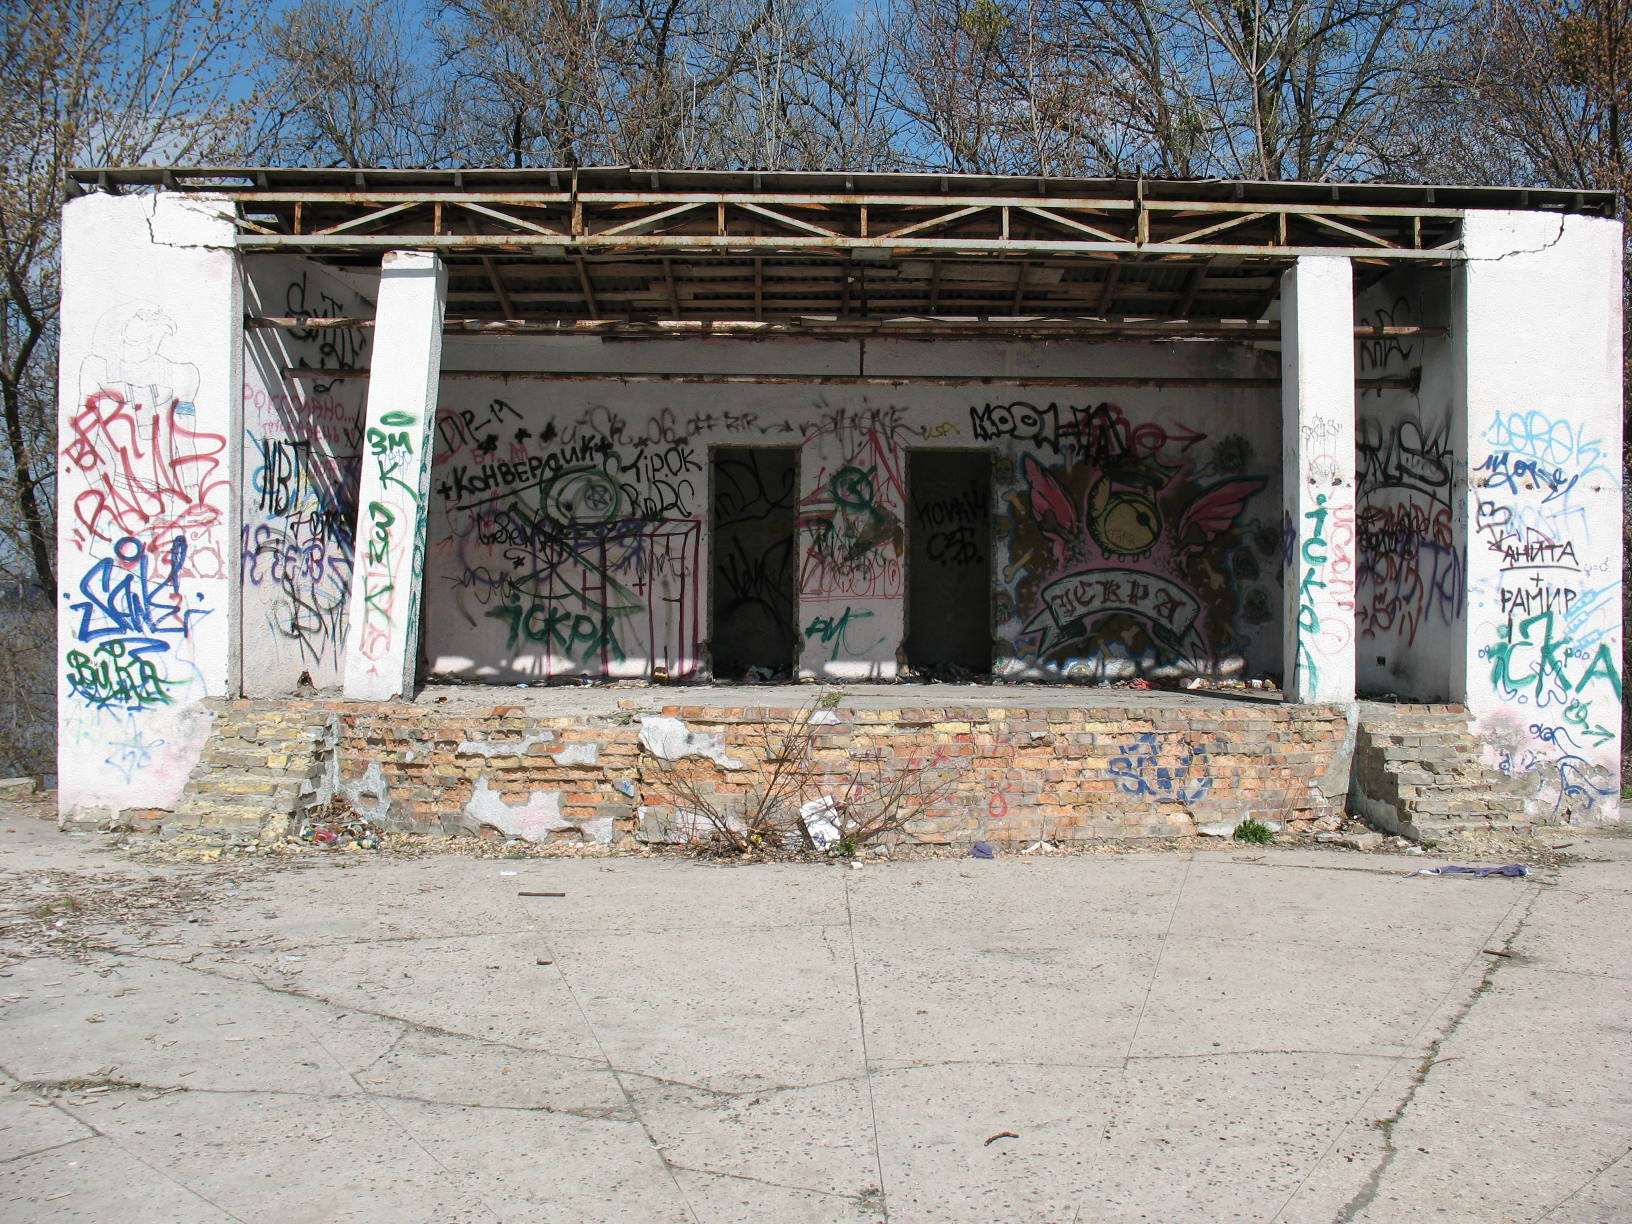
\includegraphics[width=\linewidth]{rpix/IMG_1402.JPG}

\textit{Жаба. Эстрада.}
\end{center}

\newpage

\vspace*{\fill}


\begin{center}
\includegraphics[width=\linewidth]{rpix/kamenka.jpg}
\textit{Каменка и Рогостинка на карте 1746 года.}
\end{center}


\begin{center}
\includegraphics[width=\linewidth]{rpix/IMG_20150504_142738.jpg}
\textit{Каменка у истока, 2015.}
\end{center}

\vspace*{\fill}



\begin{center}
\includegraphics[width=\linewidth]{rpix/IMG_20170611_150523.jpg}
\textit{Кинь-грусть, 2017.}
\end{center}


\begin{center}
\includegraphics[width=\linewidth]{rpix/IMG_20160330_153049.jpg}
\textit{Кирилловские высоты, Иорданское кладбище.}
\end{center}



\vspace*{\fill}

\begin{center}
\includegraphics[width=\linewidth]{rpix/alb.jpg}

\textit{Клов, слева Александровская больница, эти корпуса ныне снесены, примыкали к ул. Мечникова. Наверху на заднем плане – Северная полубашня Киевская крепости, на ул. Госпитальной, существует поныне, но из-за застройки и проложенного бульвара Леси Украинки ее с этой точки больше не видно.}
\end{center}
\vspace*{\fill}

\newpage

\vspace*{\fill}
\begin{center}
\includegraphics[width=\linewidth]{rpix/klov02.jpg}

\textit{Клов, вернее, вид на него как раз с пригорка, где у нас за спиной упомянутая полубашня.}
\end{center}
\vspace*{\fill}

\newpage
\vspace*{\fill}


\begin{center}
\includegraphics[width=\linewidth]{rpix/klov03.jpg}

\textit{Клов, 1914 год – вид из центра города на Клов. Это над ним виднеется Лаврская колокольня, хотя она много дальше. Широкая грунтовая дорога, что взбирается от Клова направо на гору, к Северной полубашне – нынешняя улица Госпитальная. Это сбивает с толку, потому что на первый взгляд думаешь – прообраз бульвара Леси Украинки, а ведь он в наше время левее.}
\end{center}
\vspace*{\fill}

\newpage
\vspace*{\fill}
\begin{center}
\includegraphics[width=\linewidth]{rpix/klov-esp.jpg}

\textit{Кловица течет за забором посередине кадра. Вид на пересечение Эспланадной и Скаскаганского. Конец 19 века.}
\end{center}
\vspace*{\fill}

\newpage


\begin{center}
\includegraphics[width=0.93\linewidth]{rpix/25-04-07_1552.jpg}

\textit{Клов застраивается. 2007. Бульвар Леси Украинки.}
\end{center}


\begin{center}
\includegraphics[width=0.93\linewidth]{rpix/25-04-07_1554.jpg}

\textit{Клов застраивается. 2007. Наверху бульвар Леси.}
\end{center}

\newpage


\begin{center}
\includegraphics[width=0.93\linewidth]{rpix/25-04-07_1554.jpg}

\textit{Клов застраивается. 2007. Наверху бульвар Леси.}
\end{center}

\begin{center}
\includegraphics[width=\linewidth]{rpix/25-04-07_1553.jpg}

\textit{Клов, а тут давно застроено. 2007.}
\end{center}


\newpage
\vspace*{\fill}


\begin{center}
\includegraphics[width=\linewidth]{rpix/IMG_20190504_133527.jpg}

\textit{Клов, 2019. Устье.}
\end{center}

\begin{center}
\includegraphics[width=\linewidth]{rpix/IMG_20190504_133538.jpg}

\textit{Клов, 2019. Устье.}
\end{center}

\vspace*{\fill}


%\begin{center}
%\includegraphics[width=\linewidth]{rpix/25-04-07_1553.jpg}

%\textit{Клов, а тут давно застроено. 2007.}
%\end{center}


%\begin{center}
%\includegraphics[width=\linewidth]{rpix/IMG_20170611_145933.jpg}

%\textit{Княжая гора, 2017.}
%\end{center}

\newpage
\vspace*{\fill}

\begin{center}
\includegraphics[width=\linewidth]{rpix/IMG_20190504_133643.jpg}

\textit{Клов, 2019. Устье прежнего коллектора.}
\end{center}


\begin{center}
\includegraphics[width=\linewidth]{rpix/IMG_20190504_133659.jpg}

\textit{Клов, 2019. Урочище Пятничный Клов, место пятничной тусовки диггеров.}
\end{center}

\vspace*{\fill}

%\begin{center}

%\includegraphics[width=\linewidth]{rpix/IMG_20170611_150002.jpg}

%\textit{Княжая гора, 2017.}
%\end{center}


\newpage

\begin{center}
\includegraphics[width=\linewidth]{rpix/IMG_20170611_145933.jpg}

\textit{Княжая гора, 2017.}
\end{center}



\begin{center}
\includegraphics[width=\linewidth]{rpix/koz-bol.jpg}

\textit{Козье болото (зеленые насаждения в левой серединной части кадра)}
\end{center}



\newpage

\begin{center}
\includegraphics[width=\linewidth]{rpix/IMG_20200815_143315.jpg}

\textit{Красный дом, 2020.}
\end{center}


\begin{center}
\includegraphics[width=\linewidth]{rpix/IMG_20170411_145319.jpg}

\textit{Костопальня, 2017.}
\end{center}


%\begin{center}
%\includegraphics[width=\linewidth]{rpix/lybed-prud-ninjiy-kadet-rosh.jpg}

%\textit{Пруд на Лыбеди.}
%\end{center}


%\begin{center}
%\includegraphics[width=\linewidth]{rpix/%lyb.png}

%\textit{Лыбедь или Киянка?}
%\end{center}

%\begin{center}
%\includegraphics[width=0.95\linewidth]{rpix/%IMG_20191126_132325.jpg}

%\textit{Лыбедь, короткий отрезок старого природного русла.}
%\end{center}

\begin{center}
\includegraphics[width=0.95\linewidth]{rpix/IMG_20190616_135257.jpg}

\textit{Лыбедь вытекает из коллектора у Лысой горы.}
\end{center}


\begin{center}
\includegraphics[width=0.92\linewidth]{rpix/IMG_20191126_132719.jpg}

\textit{Лыбедь течет по рукотворному руслу к устью.}
\end{center}


\begin{center}
\includegraphics[width=0.92\linewidth]{rpix/IMG_20191126_143542.jpg}

\textit{Лыбедь течет по рукотворному руслу к устью.}
\end{center}


\begin{center}
\includegraphics[width=\linewidth]{rpix/IMG_20191126_141033_DRO.jpg}

\textit{Лыбедь, вид на устье.}
\end{center}


\begin{center}
\includegraphics[width=\linewidth]{rpix/IMG_20191126_141702_DRO.jpg}

\textit{Лыбедь, устье.}
\end{center}


\begin{center}
\includegraphics[width=\linewidth]{rpix/IMG_20191126_142103_DRO.jpg}

\textit{Лыбедь, устье.}
\end{center}


\begin{center}
\includegraphics[width=0.95\linewidth]{rpix/IMG_20170402_144928.jpg}

\textit{Монтажник, 2017.}
\end{center}



\begin{center}
\includegraphics[width=0.95\linewidth]{rpix/navod.jpg}

\textit{Наводницкий ручей. 1951, Компаниец-Киянченко Н. Д.}
\end{center}


\begin{center}
\includegraphics[width=\linewidth]{rpix/IMG_20150701_144629.jpg}

\textit{Наводничи, 2015.}
\end{center}


\begin{center}
\includegraphics[width=0.93\linewidth]{rpix/IMG_3981.JPG}

\textit{Нивка, речка, около пруда номер 15 (по ул. Ушакова и Наумовича).}
\end{center}

\begin{center}
\includegraphics[width=0.93\linewidth]{rpix/IMG_3997.JPG}

\textit{Нивка, речка, пруд номер 14 (по ул. Живописной и Верховинной).}
\end{center}


\begin{center}
\includegraphics[width=\linewidth]{rpix/IMG_4375.jpg}

\textit{Никольский старый ввоз.}
\end{center}



\begin{center}
\includegraphics[width=\linewidth]{rpix/IMG_20201109_125203.jpg}

\textit{Ореховатка. Устье. 2020}
\end{center}


\begin{center}
\includegraphics[width=\linewidth]{rpix/IMG_20201109_125811.jpg}

\textit{Ореховатка. Устье. 2020}
\end{center}




\begin{center}
\includegraphics[width=\linewidth]{rpix/pechbaz.jpg}

\textit{Печерский базар, 1912 год.}
\end{center}


\begin{center}
\includegraphics[width=\linewidth]{rpix/IMG_20201109_125816.jpg}

\textit{Пещера Белых сталактитов, вход. 2020.}
\end{center}




\begin{center}
\includegraphics[width=\linewidth]{rpix/IMG_20190504_141816.jpg}

\textit{Протасов яр, 2019. Наверху, вид на Соломенку.}
\end{center}


\begin{center}
\includegraphics[width=\linewidth]{rpix/IMG_20190504_141817.jpg}

\textit{Протасов яр, 2019. На горе, вид на верховье яра.}
\end{center}


\begin{center}
\includegraphics[width=0.90\linewidth]{rpix/DSC_0022.JPG}

\textit{Пятачок, 2007 год. Вид в сторону Бастионной.}
\end{center}


\begin{center}
\includegraphics[width=0.90\linewidth]{rpix/DSC_0021.JPG}

\textit{Пятачок, 2007 год. Вид в сторону Бастионной и «Дары Ланив».}
\end{center}



\begin{center}
\includegraphics[width=0.95\linewidth]{rpix/IMG_20130826_173616.jpg}

\textit{Пятачок, во дворах, 2013 год.}
\end{center}



\begin{center}
\includegraphics[width=\linewidth]{rpix/repyar.jpg}

\textit{Репяхов яр с проложенным по нему Кирилловским спуском. Далее спуск был переименован во Врубелевский и практически исчез.}
\end{center}


\begin{center}
\includegraphics[width=\linewidth]{rpix/repyar1908.jpg}

\textit{Репяхов яр, 1908 год.}
\end{center}


\begin{center}
\includegraphics[width=\linewidth]{rpix/IMG_4332.JPG}

\textit{Рогостинка, 2015.}
\end{center}


\begin{center}
\includegraphics[width=0.95\linewidth]{rpix/imag0041.jpg}

\textit{Собачка, 2005. Наверху, вид на забор ботсада.}
\end{center}


\begin{center}
\includegraphics[width=0.95\linewidth]{rpix/imag0044.jpg}

\textit{Собачка, 2005. Верхняя тропа вдоль забора ботсада.}
\end{center}


\begin{center}
\includegraphics[width=\linewidth]{rpix/imag0052.jpg}

\textit{Собачка, 2005. Остатки спортплощадки.}
\end{center}



\begin{center}
\includegraphics[width=\linewidth]{rpix/IMG_4319.jpg}

\textit{Сырец.}
\end{center}


\begin{center}
\includegraphics[width=\linewidth]{rpix/DSC_0016.JPG}

\textit{«Темп», бывший, конечно. Фото 2007 года.}
\end{center}



\begin{center}
\includegraphics[width=\linewidth]{rpix/IMG_20210601_134915.jpg}

\textit{Тропа Хо Ши Мина. 2021. Начало.}
\end{center}



\begin{center}
\includegraphics[width=\linewidth]{rpix/IMG_20210601_134927.jpg}

\textit{Тропа Хо Ши Мина. 2021. Подошли и смотрим в низину.}
\end{center}



\begin{center}
\includegraphics[width=\linewidth]{rpix/IMG_20210601_134940.jpg}

\textit{Тропа Хо Ши Мина. 2021. Подошли и смотрим в низину.}
\end{center}



\begin{center}
\includegraphics[width=\linewidth]{rpix/IMG_20210601_134942.jpg}

\textit{Тропа Хо Ши Мина. 2021. Подошли и смотрим в низину.}
\end{center}



\begin{center}
\includegraphics[width=\linewidth]{rpix/IMG_20210601_134945.jpg}

\textit{Тропа Хо Ши Мина. 2021. Подошли и смотрим в низину.}
\end{center}



\begin{center}
\includegraphics[width=\linewidth]{rpix/IMG_20210601_135238.jpg}

\textit{Тропа Хо Ши Мина. 2021. Подошли и смотрим в низину.}
\end{center}


\begin{center}
\includegraphics[width=\linewidth]{rpix/IMG_20210601_135245.jpg}

\textit{Тропа Хо Ши Мина. 2021. Подошли и смотрим в низину.}
\end{center}



\begin{center}
\includegraphics[width=\linewidth]{rpix/IMG_20210601_135248.jpg}

\textit{Тропа Хо Ши Мина. 2021. Подошли и смотрим в низину.}
\end{center}



\begin{center}
\includegraphics[width=\linewidth]{rpix/IMG_20210601_135253.jpg}

\textit{Тропа Хо Ши Мина. 2021. Подошли и смотрим в низину.}
\end{center}



\begin{center}
\includegraphics[width=\linewidth]{rpix/IMG_20210601_135258.jpg}

\textit{Тропа Хо Ши Мина. 2021. Подошли и смотрим в низину.}
\end{center}


\begin{center}
\includegraphics[width=0.95\linewidth]{rpix/imag0031.jpg}

\textit{Черная гора, застройка над озером Глинка, 2005 год.}
\end{center}


\begin{center}
\includegraphics[width=0.95\linewidth]{rpix/IMG_20160828_145726.jpg}

\textit{Чертова долина (ул. Соляная), 2016.}
\end{center}

\begin{center}
\includegraphics[width=\linewidth]{rpix/IMG_20160828_145732.jpg}

\textit{Чертова долина (ул. Соляная), 2016.}
\end{center}



\begin{center}
\includegraphics[width=\linewidth]{rpix/meringa_usadba.jpg}

\textit{Усадьба Меринга, 1870-е годы, фото Франц де Мезер}
\end{center}


\begin{center}
\includegraphics[width=\linewidth]{rpix/meringa_usadba.jpg}

\textit{Усадьба Меринга, 1870-е годы, фото Франц де Мезер.}
\end{center}


\begin{center}
\includegraphics[width=\linewidth]{rpix/IMG20101126_003.jpg}

\textit{Фрометовка.}
\end{center}



\begin{center}
\includegraphics[width=\linewidth]{rpix/04092010908.jpg}

\textit{Ширма, ул. Казачья.}
\end{center}




\begin{center}
\includegraphics[width=\linewidth]{rpix/IMG_20130614_142415.jpg}

\textit{Ширма, ул. Казачья.}
\end{center}


\begin{center}
\includegraphics[width=\linewidth]{rpix/IMG_20130826_173246.jpg}

\textit{Яма, 2013 год.}
\end{center}




%\part{Архитекторы}

%\input{ludi/ermakov.tex}



\backmatter


%\begin{thebibliography}{999}
%\input{bibitems}
%\end{thebibliography}

\newpage

\pagestyle{empty}

\clearpage
\vspace*{\stretch{2}}
\begin{center}
\begin{minipage}{\textwidth}
\begin{center}Спасибо, что дочитали до этой страницы\end{center}
\end{minipage}
\end{center}
\vspace{\stretch{3}}
\clearpage

%\vfill

%тираж ОГРОМНЫЙ

\end{document} 